%%%%%%%%%%%%%%%%%%%%%%%%%%%%%%%%%%%%%%%%%
% Masters/Doctoral Thesis 
% LaTeX Template
% Version 2.5 (27/8/17)
%
% This template was downloaded from:
% http://www.LaTeXTemplates.com
%
% Version 2.x major modifications by:
% Vel (vel@latextemplates.com)
%
% This template is based on a template by:
% Steve Gunn (http://users.ecs.soton.ac.uk/srg/softwaretools/document/templates/)
% Sunil Patel (http://www.sunilpatel.co.uk/thesis-template/)
%
% Template license:
% CC BY-NC-SA 3.0 (http://creativecommons.org/licenses/by-nc-sa/3.0/)
%
%%%%%%%%%%%%%%%%%%%%%%%%%%%%%%%%%%%%%%%%%

%----------------------------------------------------------------------------------------
%	PACKAGES AND OTHER DOCUMENT CONFIGURATIONS
%----------------------------------------------------------------------------------------

\documentclass[
11pt, % The default document font size, options: 10pt, 11pt, 12pt
%oneside, % Two side (alternating margins) for binding by default, uncomment to switch to one side
english, % ngerman for German
singlespacing, % Single line spacing, alternatives: onehalfspacing or doublespacing
%draft, % Uncomment to enable draft mode (no pictures, no links, overfull hboxes indicated)
%nolistspacing, % If the document is onehalfspacing or doublespacing, uncomment this to set spacing in lists to single
%liststotoc, % Uncomment to add the list of figures/tables/etc to the table of contents
%toctotoc, % Uncomment to add the main table of contents to the table of contents
%parskip, % Uncomment to add space between paragraphs
%nohyperref, % Uncomment to not load the hyperref package
headsepline, % Uncomment to get a line under the header
%chapterinoneline, % Uncomment to place the chapter title next to the number on one line
%consistentlayout, % Uncomment to change the layout of the declaration, abstract and acknowledgements pages to match the default layout
]{MastersDoctoralThesis} % The class file specifying the document structure

\usepackage[utf8]{inputenc} % Required for inputting international characters
\usepackage[T1]{fontenc} % Output font encoding for international characters

%\usepackage{mathpazo} % Use the Palatino font by default
%\usepackage{mathtools}
\usepackage{amsmath}
\usepackage{xspace} 

%\usepackage[backend=biber,style=authoryear,natbib=true]{biblatex} % Use the bibtex backend with the authoryear citation style (which resembles APA)
%\bibliographystyle{unsrt}
%\usepackage[style=phys, articletitle=false,biblabel=brackets, chaptertitle=false,pageranges=false]{biblatex}
%\addbibresource{bibliography.bib} % The filename of the bibliography

\usepackage[autostyle=true]{csquotes} % Required to generate language-dependent quotes in the bibliography
%for making reference ranges appeaer as they should
\usepackage[utf8]{inputenc}
\usepackage{cite}
\usepackage[compat=1.0.0]{tikz-feynman}
%----------------------------------------------------------------------------------------
%	MARGIN SETTINGS
%----------------------------------------------------------------------------------------

\geometry{
	paper=a4paper, % Change to letterpaper for US letter
	inner=2.cm, % Inner margin
	outer=3.3cm, % Outer margin
	bindingoffset=.5cm, % Binding offset
	top=2.5cm, % Top margin
	bottom=2.5cm, % Bottom margin
	%showframe, % Uncomment to show how the type block is set on the page
}

%----------------------------------------------------------------------------------------
%	THESIS INFORMATION
%----------------------------------------------------------------------------------------

\thesistitle{Search for heavy neutral leptons in events with three charged leptons
 in pp collision at $\sqrt s = 13$ TeV at CMS detector} % Your thesis title, this is used in the title and abstract, print it elsewhere with \ttitle
\supervisor{Prof Dr. Didar \textsc{Dobur}} % Your supervisor's name, this is used in the title page, print it elsewhere with \supname
\examiner{} % Your examiner's name, this is not currently used anywhere in the template, print it elsewhere with \examname
\degree{Doctor of Philosophy} % Your degree name, this is used in the title page and abstract, print it elsewhere with \degreename
\author{Martina \textsc{Vit}} % Your name, this is used in the title page and abstract, print it elsewhere with \authorname
\addresses{} % Your address, this is not currently used anywhere in the template, print it elsewhere with \addressname

\subject{High Energy Particle Physics} % Your subject area, this is not currently used anywhere in the template, print it elsewhere with \subjectname
\keywords{} % Keywords for your thesis, this is not currently used anywhere in the template, print it elsewhere with \keywordnames
\university{\href{https://www.ugent.be/nl}{Universiteit Gent}} % Your university's name and URL, this is used in the title page and abstract, print it elsewhere with \univname
\department{\href{https://www.ugent.be/we/physics-astronomy/en}{Department of Physics and Astronomy}} % Your department's name and URL, this is used in the title page and abstract, print it elsewhere with \deptname
\group{\href{https://epp.ugent.be/}{Experimental Particle Physics}} % Your research group's name and URL, this is used in the title page, print it elsewhere with \groupname
\faculty{\href{http://faculty.university.com}{Faculty Name}} % Your faculty's name and URL, this is used in the title page and abstract, print it elsewhere with \facname

\AtBeginDocument{
\hypersetup{pdftitle=\ttitle} % Set the PDF's title to your title
\hypersetup{pdfauthor=\authorname} % Set the PDF's author to your name
\hypersetup{pdfkeywords=\keywordnames} % Set the PDF's keywords to your keywords
\hypersetup{urlcolor= ugblue}
}


\begin{document}

\frontmatter % Use roman page numbering style (i, ii, iii, iv...) for the pre-content pages

\pagestyle{plain} % Default to the plain heading style until the thesis style is called for the body content
%----------------------------------------------------------------------------------------
%	TITLE PAGE
\begin{titlepage}

\includegraphics[height=4cm]{Figures/logo_Ugent}\\

\begin{center}
\vspace*{.01\textheight}
{\scshape\huge \univname\par}\vspace{1.5cm} % University name
\textsc{\Large Doctoral Thesis}\\[0.5cm] % Thesis type

\HRule \\[0.4cm] % Horizontal line
{\huge \bfseries \ttitle\par}\vspace{0.4cm} % Thesis title
\HRule \\[1.5cm] % Horizontal line
 
\begin{minipage}[t]{0.4\textwidth}
\begin{flushleft} \Large
\emph{Author:}\\
{\authorname} % Author name - remove the \href bracket to remove the link
\end{flushleft}
\end{minipage}
\begin{minipage}[t]{0.4\textwidth}
\begin{flushright} \Large
\emph{Supervisor:} \\
{\supname} % Supervisor name - remove the \href bracket to remove the link  
\end{flushright}
\end{minipage}\\[1cm]
 
\vspace{8mm}

\large \textit{A thesis submitted in fulfillment of the requirements\\ for the degree of \degreename}\\[0.3cm] % University requirement text
\textit{in the}\\[0.4cm]
\groupname\\\deptname\\[3cm] % Research group name and department name
 
\vspace{4mm}

{\large \today}\\[1cm] % Date
%\includegraphics{Logo} % University/department logo - uncomment to place it
\end{center}
\end{titlepage}
%----------------------------------------------------------------------------------------
%	DECLARATION PAGE
%\begin{declaration}
\addchaptertocentry{\authorshipname} % Add the declaration to the table of contents
\noindent I, \authorname, declare that this thesis titled, \enquote{\ttitle} and the work presented in it are my own. I confirm that:

\begin{itemize} 
\item This work was done wholly or mainly while in candidature for a research degree at this University.
\item Where any part of this thesis has previously been submitted for a degree or any other qualification at this University or any other institution, this has been clearly stated.
\item Where I have consulted the published work of others, this is always clearly attributed.
\item Where I have quoted from the work of others, the source is always given. With the exception of such quotations, this thesis is entirely my own work.
\item I have acknowledged all main sources of help.
\item Where the thesis is based on work done by myself jointly with others, I have made clear exactly what was done by others and what I have contributed myself.\\
\end{itemize}
 
\noindent Signed:\\
\rule[0.5em]{25em}{0.5pt} % This prints a line for the signature
 
\noindent Date:\\
\rule[0.5em]{25em}{0.5pt} % This prints a line to write the date
\end{declaration}
%\cleardoublepage
%----------------------------------------------------------------------------------------
%	QUOTATION PAGE

\vspace*{0.2\textheight}

\noindent\enquote{\itshape That is fundamentally the only courage which is demanded of us: to be brave in the face of the strangest, most singular and most inexplicable things that can befall us. The fact that human beings have been cowardly in this sense has done endless harm to life; the experiences that are called “apparitions”, the whole of the so-called “spirit world”, death, all these things that are so closely related to us, have been so crowded out of life by our daily warding them off, that the senses by which we might apprehend them are stunted. To say nothing of God. But fear of the inexplicable has not only impoverished the existence of the solitary man, it has also circumscribed the relationships between human beings, as it were lifted them up from the river bed of infinite possibilities to a fallow spot on the bank, to which nothing happens.}\bigbreak

\hfill Rainer Maria Rilke


%----------------------------------------------------------------------------------------
%	ABSTRACT PAGE

\begin{abstract}
\addchaptertocentry{\abstractname} % Add the abstract to the table of contents
The Thesis Abstract is written here (and usually kept to just this page). The page is kept centered vertically so can expand into the blank space above the title too\ldots
\end{abstract}


%----------------------------------------------------------------------------------------
%	LIST OF CONTENTS PAGES
\tableofcontents % Prints the main table of contents

%----------------------------------------------------------------------------------------
%	DEDICATION
%----------------------------------------------------------------------------------------
\dedicatory{For/Dedicated to/To my\ldots} 
%----------------------------------------------------------------------------------------
%	THESIS CONTENT - CHAPTERS
%----------------------------------------------------------------------------------------
\mainmatter % Begin numeric (1,2,3...) page numbering

\pagestyle{thesis} % Return the page headers back to the "thesis" style
%\chapter*{Introduction}\label{chapter:introduction}
%\setcounter{page}{0}
%\pagenumbering{arabic}
%from here on, start the 'real' page numbering, from 1, with normal digits
\chapter*{Preface}\label{chapter:introduction}
\enquote{\itshape {\small We do not know what the rules of the game are; all we are allowed to
do is to watch the playing. Of course, if we watch long enough, we may
eventually catch on to a few of the rules. The rules of the game are
what we mean by fundamental physics.}} Richard P. Feynman\\

This quote brilliantly exemplifies the need for fundamental
research. We all want to satisfy our 
curiosity and science is a process of investigating, keeping on
questioning, and trying to uncover the unresolved.\\
Thus, the need for the construction
of huge laboratories where to study the fundamental constituents of
matter becomes explicit.
CERN's accelerator complex and experiments are the
best place to ``watch the playing'' and ``if we watch long enough, we may
eventually catch on to a few of the rules''.

Since the 1960s, physicists had proposed a collection of what
they assumed to be the fundamental particles and the fundamental forces
 that govern the interaction between particles themselves. This was
 the start of the development of the Standard Model (SM) of particle
 physics. At CERN we make use of the world's
most potent particle accelerators and experiments to question the
predictions and to test limits of the Standard Model. So far,
the Standard Model has favorably described and predicted
approximately all experimental outcomes till the latest
discoveries such as top quark observation (1995)~\cite{Abachi_1995}
and Higgs boson discovery (2012)~\cite{20121,201230}.

However, cosmological and astronomical observations, together with theoretical
considerations allude to physics beyond the Standard Model
(BSM). Furthermore, the observation of neutrino flavor oscillations was one of the first 
definite experimental indications for the
presence of new physics not described by the SM theory.
 Therefore, it felt crucial to investigate the signatures of different
 BSM models at the LHC
experiments
to try spotting the mysterious new physics. Above all, comprehending the
mechanism that discloses the neutrino mass would be a
vital glance into ``the rules of the game''.

The two results presented in this dissertation cooperate in the arduous attempt of confronting exotic BSM
models with the experimental data. The aim is to find new
physics that is able to describe the unexplained
physics observations not covered by the SM.\\

This thesis tries to give an overview of all the steps needed to follow
to experimentally investigate physics
beyond the Standard Model. The reader will encounter respectively the
descriptions of: theoretical models and predictions, experimental
layout, detector performances, data analysis and unfortunately, at the
end not a discovery but exclusion limits on specific exotic models.

After a brief description of the principles of the Standard Model in
Chapter~\ref{Chapter1}, a summary of the Large Hadron Collider (LHC)
and of the Compact Muon Solenoid (CMS) components and objectives is
presented in Chapters~\ref{Chapter2} and~\ref{Chapter2_5}.\\
In Chapter~\ref{Chapter3} the main topic of the doctoral project is
introduced. The focus is on the right-handed (RH) neutrino or heavy
neutral lepton (\hnl or HNL)
model. In Chapters~\ref{Chapter1} and~\ref{Chapter3} 
the relevance and the interest for the
ongoing HNL search program is illustrated, describing first the theory setting 
and then mentioning the various of experiments and results
focusing on HNL.

Two separated searches on HNLs have been performed using the data
collected by the CMS detector. The two analyses are the core of this
dissertation.\\
The HNL searches are fully described in Chapters~\ref{Chapter5}
and~\ref{Chapter6} and they target complementary phase spaces in HNL mass, $m_\hnl$
and mixing parameter, \mixpar, between heavy neutrinos and standard
model neutrinos. The study focuses first on the
moderate and high mass search and then drifts to very low mass search with
the introduction of a long-lived HNL scenario.

In Chapter~\ref{Chapter5}, the search for heavy neutral leptons with three
prompt charged leptons in any flavor combination of electrons and
muons is defined. It results in a comprehensive analysis that probes the production of the
\hnl in an extended mass range never investigated before at the LHC:
from 1\GeV, and up to 1.2\TeV. 
Organized into two parts, the search is optimized for
probing HNLs of masses respectively above and below that of the \PW
boson. Several analysis techniques are introduced.

In Chapter~\ref{Chapter6}, the search for long-lived heavy neutral
leptons is presented. The analysis signature
consisting of one prompt charged lepton and two displaced
charged leptons originating from the secondary vertex of the \hnl
decay. Due to its unconventional signature, the whole analysis process has been
quite demanding; several challenges are presented (final part of
Chapter~\ref{Chapter4} as well) and the steps taken during the three
year course are inspected and described one by one.

In Chapter~\ref{Chapter7}, a short summary is given together with an
inclusive outlook overview. The future prospects section tries to give a feeling of the vast landscape
where the two CMS HNL searches sit. The idea is to give a sense of the
context and of the perspective from which one should look at these results.

\subsection*{Author's contribution}

The author contributed to the development and finalization of the
searches for heavy neutral leptons in multilepton final
states at CMS.\\
The precise contributions of the author are specified at
the end of the two dedicated chapters
(~\ref{Chapter5},~\ref{Chapter6}) 
and are summarized shortly below.\\

For almost the first two years of the PhD, the author
has participated in the search for heavy neutral leptons with three
prompt charged leptons in any flavor combination of electrons and
muons. \\
The analysis
results were published in Physical Review Letters in early 2018:
\begin{itemize}
\setlength\itemsep{-0.1em}
\item CMS Collaboration, \emph{Search for heavy neutral leptons in events with three charged leptons
in proton-proton collisions at $\sqrt{s}$ = 13 TeV}. Phys. Rev. Lett., 120(22):221801, 2018.
\end{itemize}

The results discussed in Chapter~\ref{Chapter5} were presented by the author at the following
conferences:
\begin{itemize}
\setlength\itemsep{-0.1em}
\item (YSF talk) Search for heavy neutral leptons (sterile
  neutrinos) with the CMS detector, plenary at La Thuile 2018, 25
  Feb-3 Mar 2018 (Italy);
\item Search for Heavy Neutral Leptons with CMS detector, poster at
  EPS-HEP2019, 10-17 Jul 2019 (Belgium);
\item Search for Heavy Neutral Leptons with CMS detector, poster at
  LP2019, 5-10 Aug 2019, University of Toronto (Canada);
\item HNL experimental overview, plenary at EOS Winter Solstice
  meeting, 19 Dec 2019, Brussels (Belgium);
\item  Search for heavy neutral leptons at CMS, parallel at
  ICHEP2020, 28 Jul-6 Aug 2020 (Virtual World).
\end{itemize}
The poster presented at EPS-HEP2019 was awarded ``poster prize of
the EPS High Energy and Particle Physics Division and the EPS HEP 2019
Conference''.\\
 
In the last three years of PhD the author was the main developer for the
long-lived heavy neutral lepton search. \\
The analysis results have been collected in the Physics Analysis
Summaries, PAS which has been made public. The final paper will be
submitted by the end of the year to Journal
of High Energy Physics (JHEP):
\begin{itemize}
\setlength\itemsep{-0.1em}
\item CMS Collaboration, \emph{Search for long-lived heavy neutral leptons with displaced vertices in pp collisions at $\sqrt{s}$ =
13TeV with the CMS detector}. Technical report, CERN, Geneva, 2021.
\end{itemize}

The results discussed in Chapter~\ref{Chapter6} were presented by the author at the following
conferences and workshops:

\begin{itemize}
\setlength\itemsep{-0.1em}
\item HNL experimental overview, talks Searching for long-lived
  particles at the LHC: firth workshop of the LHC LLP Community, 27-29
  May 2019, CERN (Switzerland);
\item HNL experimental overview', plenary at EOS winter Solstice
  meeting, 19 Dec 2019, Brussels (Belgium);
\end{itemize}

At the European Physical Society Conference on High Energy Physics
(EPS-HEP) in July 2021, the results were for the first time publicly
presented by CMS Physics Coordinator in ``Highlights from the CMS
Experiment'' talk.



\addcontentsline{toc}{chapter}{Introduction}

\clearpage

% Include the chapters of the thesis as separate files from the Chapters folder
% Uncomment the lines as you write the chapters
% Chapter Template
\part{Physics introduction}
\chapter{The Standard Model and Beyond} \label{Chapter1} 

\section{Introduction}
Starting from the late 19th century and progressing in the first half of the 20th century, 
the theories and discoveries of thousands of physicists have led to a significant insight into the fundamental structure of matter. 
By the 1960s, physicists had proposed quite a collection of what they assumed to be fundamental particles, basic building blocks of matter that could not be resolved any further into sub-pieces. 

In 1964, theorists Murray Gell-Mann~\cite{GELLMANN1964214} and George Zweig~\cite{Zweig:570209} theorized that many components of the so-called ``particle zoo'' were composite particles which consists of even smaller parts, which are now called quarks. Thus the list of fundamental particles was further reduced and the description of the fundamental forces which govern the interaction between particles themselves was added. This was the outset of the development of the Standard Model of particle physics.
The first references to the so-called “standard model” can be found in papers published in the 1970s~\cite{Pais:1975gn,PhysRevD.13.680} and only in the '80s and '90s the \emph{S} and \emph{M} got capitalized.

To this day, the Standard Model (SM) has successfully interpreted nearly all experimental results and accurately predicted a wide variety of phenomena, getting even more credit with the latest discoveries such as top quark observation (1995)~\cite{Abachi_1995} and Higgs boson discovery (2012)~\cite{20121,201230}.\\
Even though it is considered the most solid description of the subatomic world, we see some inconsistencies when trying to address the full picture. Those unexplained physisc observations have inspired the big hunt for new physics that has drawn the creation of so many new experiments and that has fed fresh exotic theories. This thesis cooperates in this attempt.


\section{The Standard Model of Elementary Particles}\label{sec:sm}
Figure~\ref{fig:SMfig} shows the building blocks of the Standard Model. They are either matter particles, everyday matter
or exotic matter created in particle accelerators and in the early universe, or they are the additional force-carrier particles.

In the Standard Model, the elementary particles are grouped into two main categories on the basis of the statistic they obey and consequently of the spin: fermions and bosons. 
\begin{figure}[h]
\centering
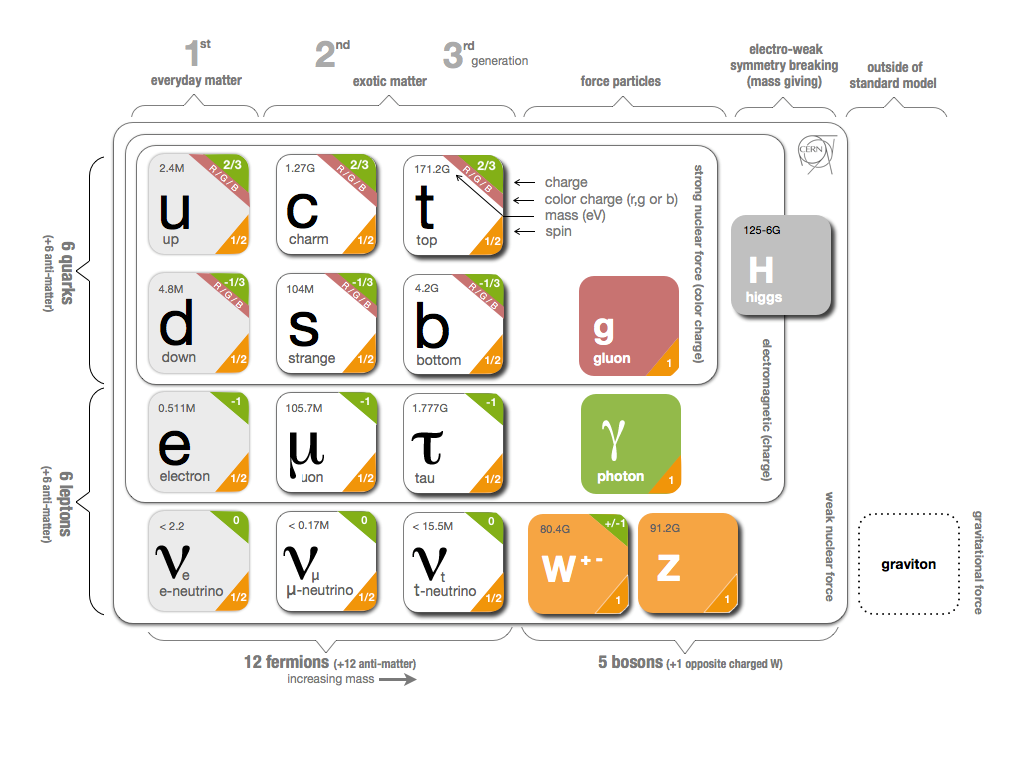
\includegraphics[clip,trim=1cm 2cm 2cm 1cm, width=0.75\textwidth]{Figures/c1/SMinfographic_image.png}
\caption{Elementary particles of the Standard Model (infographic
  developed for~\cite{particlefest})}
\label{fig:SMfig}
\end{figure}

The fermions are particles which follow Fermi-Dirac statistics and correspondingly have half odd integer spin (1/2, 3/2, 5/2...). They obey the Pauli exclusion principle and therefore they have different symmetry properties, with respect to bosons, when exchanging of two identical particles: the total wave function of a system of two identical fermions is antisymmetric for fermions. This leads to the fact that, in a rigorous way, if two identical (in spin and space coordinates) fermions interchange, the total wave function changes its sign. Thus, two or more identical fermions can not simultaneously exist in the same quantum state. On the contrary particles with an integer spin like the bosons which follow Bose-Einstein statistics do not obey the Pauli exclusion principle and can occupy the same quantum state. 


In the Standard Model, there are two types of elementary fermions: quarks (which form hadrons such as protons and neutrons) and leptons. 
Moreover, the fermions are grouped into three generations and each generation has two types of leptons and two quarks. One of the two leptons have one electric charge -1, the other one is neutral; the two quarks have charges $-1/3$ (down-type) and $+2/3$ (up-type). Between generations electric and strong interactions are identical while particles differ by their flavor quantum number and mass.  The first generation consists of electrons ($e$) and electron neutrinos ($\nu_e$) and of \emph{up} and \emph{down} quarks. All the everyday matter is composed by up-down quarks and electrons. The second generation is made of muons ($\mu$) and muon neutrinos ($\nu_\mu$) and of \emph{charm} and \emph{strange} quarks. The third generation is composed by taus ($\tau$) and tau neutrino ($\nu_\tau$) and by \emph{top} and \emph{bottom} quarks. The particles of higher generations have larger masses than the preceding ones, this has the effect that leptons and quarks of the second and third families are more unstable with shorter life-times and can easily decay back to elements from the first generation.\\
Each of the 12 fermions has an anti-matter particle which presents all the charges with opposite sign.

The fermions interact by exchanging bosons. The elementary bosons are force carriers and each of them is associated with a fundamental force. The photon ($\gamma$) is the mediator of the electromagnetic force, it has spin equal to 1, it is neutral and massless. The $\PW^{\pm}$ and \PZ are mediators of the weak force, they have spin 1, the $\PW^{\pm}$ have unitary charge (+1 or -1) while \PZ is neutral; the are heavy in mass ($M_\PW =\:$80.379 $\pm$ 0.012\GeV~\cite{pdgw}, $M_\PZ =\:$91.1876 $\pm$ 0.0021\GeV~\cite{pdgz}) and very short-lived. The quarks possess color charge which means they are subject to the strong interaction mediated by the gluons ($g$) which likewise are associated to a color charge. Because of a property of the strong interaction known as \emph{color confinement}, quarks can not exist isolated. Therefore quarks and gluons must cluster together to form hadrons which are color neutral (white) and which can exist and propagate freely. The hadrons can be made of either a quark and an anti-quark, \emph{mesons} or three quarks, \emph{baryons}. The mesons are composite bosons (spin 0 or 1) while baryons are composite fermions. Quarks, besides interacting through strong force, can also transform into quarks of another flavor through the weak interaction by absorbing/emitting a \PW boson. The strengths/probabilities of the weak interactions between the six quarks do not have all the same magnitude (some are more preferable) and they are described by the values in the Cabibbo–Kobayashi–Maskawa matrix~\cite{10.1143/PTP.28.870}.\\
The massive bosons get their mass thanks to the interaction with the quantum field. The so-called Brout–Englert–Higgs (BEH) mechanism refers to the generation of masses for the three weak gauge bosons (\PW, \PZ) through electroweak symmetry breaking~\cite{PhysRevLett.13.321,PhysRevLett.13.508}. The mathematical treatment of the Standard Model and of the BEH mechanism is presented in Sec.\ref{sec:mathSM}.\\
The last fundamental force, gravity, is not included in the Standard Model framework. 

The leptons are not affected by the strong interaction while they are subject to electromagnetic and weak interactions. As already said, the six leptons are organized in three generations, then are arranged in three left-handed weak isospin doublets where charged and neutral leptons share the same left-handed helicity. Each doublet has a different lepton number which has to be conserved during all the interactions implying that leptons and anti-leptons must be created in pairs of a single generation. The only violation of this universal lepton number conservation can be observed in the weak interaction in the neutrino oscillations where is there a transformation between different generations. The neutrino oscillation and the obvious consequences are going to be extensively explained in Sec.~\ref{sec:bsm}. 


\section{The mathematical formulation of the Standard Model}\label{sec:mathSM}
This section describes the mathematical framework of the Standard Model of particle physics, which is a gauge Quantum Field Theory (\emph{QFT}). For an extensive discussion and explanation of QFT and of the Standard Model I refer to~\cite{Bardin:1999ak}.
\subsection{Quantum Field Theory and Gauge invariance}\label{sec:qft}
In a QFT theory, the fundamental objects are described as quantum fields with specific transformation properties governed by a set of symmetry groups. The fields are: the \emph{fermion} fields $\psi$, the \emph{electroweak boson} fields $W_1, \; W_2, \; W_3,$ and $B$, the \emph{gluon} field $G_a$ and the Higgs field $\phi$. The dynamics of those quantum fields are completely determined by the Lagrangian density, $\mathcal{L}$. \\
The description of QFT starts with a Lagrangian density $\mathcal{L}$, a function of the fields in the system and their derivatives, and possibly the space-time coordinates; minimizing the action ($\mathcal{S}$), which is the space-time integral of $\mathcal{L}$, the equation of motion can be extracted:
\begin{equation}
\label{eq:action}
 \mathcal{S} \;\; = \;\; \int \mathcal{L}(x) \ d^4x,
\end{equation}
where x is the space-time coordinate.

The complete Standard Model Lagrangian contains specific terms for every one of the fundamental interactions. In the rest of the section all these elements and the corresponding meanings are going to be illustrated and clarified.

To start, consider the Lagrangian of a free spinor field $\psi$ which contains a kinetic and mass term:
\begin{equation}
\label{eq:dirac}
 \mathcal{L}_{Dirac} \;\; = \;\; \overline{\psi}(x)\ (i\gamma^{\mu}\partial_{\mu} - m ) \psi(x)
\end{equation}
where the Einstein notation is used which implies summation over the indices $\mu \in 0,1,2,3$; $m$ is the fermion's mass, $\gamma^{\mu}$ are the gamma matrices ($\gamma^{\mu}\gamma^{\nu} + \gamma^{\nu}\gamma^{\mu} = 2g^{\mu\nu}$ with $g^{\mu\nu}$ is the Minkowski metric) and $\partial_{\mu}$ is the space-time derivative $(\nicefrac{\partial}{\partial_{t}}, \nicefrac{\partial}{\partial_{x}}, \nicefrac{\partial}{\partial_{y}}, \nicefrac{\partial}{\partial_{z}})$. The $\psi(x)$ denotes the Dirac fermion field and the anti-fermion field, the adjoint spinor $\overline{\psi}(x)$ is defined as $\psi^\dag\gamma^{0}$, with $\psi^\dag$ the hermitian conjugate of $\psi$.

The Standard model is a gauge quantum field theory which means it is based on the hypothesis that some symmetries, \ie transformations that leave the Lagrangian of the system unchanged, are possible not only globally, but also locally.
Most theories of physics are described by Lagrangians who are invariant under certain transformations of the coordinate system performed simultaneously at every point in spacetime: they are therefore said to have global symmetries. A local symmetry is one that keeps a property invariant when a possibly different symmetry transformation is applied at each point of spacetime; specifically a local symmetry transformation is parameterized by the spacetime co-ordinates, whereas a global symmetry is not. The concept underlying gauge theories is precisely the postulate that Lagrangians must also possess local symmetries, i.e. gauge symmetries and gauge invariant.\\
Going back to Eq.~\ref{eq:dirac}, this Lagrangian is invariant under a global U(1) phase transformation
\begin{equation}
\label{eq:globalT}
 \psi(x) \rightarrow \psi'(x) = e^{-i\omega} \psi(x), \; \; \; \; \; \;    \overline{\psi}(x) \rightarrow \overline{\psi'}(x) = e^{i\omega} \overline{\psi}(x),
\end{equation}
where $\omega$ is a constant. Thus, the requirement is for this Lagrangian to be invariant under a local U(1) transformation
\begin{equation}
\label{eq:localT}
 \psi(x) \rightarrow \psi'(x) = e^{-i\omega(x)} \psi(x), \; \; \; \; \; \;    \overline{\psi}(x) \rightarrow \overline{\psi'}(x) = e^{i\omega(x)} \overline{\psi}(x),
\end{equation}
where now $\omega(x)$ is a function of the spacetime point $x$. Considering then that $\partial_{\mu}$ would also act on $\omega(x)$, to make the 
Lagrangian invariant under this gauge symmetry, a new term, vector field, $A_{\mu}$ has to be introduced in Eq.~\ref{eq:dirac}:
\begin{equation}
\label{eq:GS1}
 \mathcal{L}_{Dirac} \;\; = \;\; \overline{\psi} (i\gamma^{\mu} (\partial_{\mu} + igA_{\mu})-m) \psi \;\;\; \equiv  \;\;\; \overline{\psi} (i\gamma^{\mu}\mathcal{D}_{\mu}-m) \psi 
\end{equation}
(the $(x)$ dependence is omitted from the notation).\\
 $A_{\mu}$ is the gauge field which couples to the spinor field $\psi$ with a coupling strength $g$; $\mathcal{D}_{\mu}$ is called covariant derivate and it is defined as $\mathcal{D}_{\mu} = \partial_{\mu} + igA_{\mu}$. \\
The $\mathcal{L}_{Dirac}$ in Eq.~\ref{eq:GS1} is invariant under local trasformation ($\mathcal{L}_{\psi} =\mathcal{L}_{\psi'}$) requiring:
\begin{equation}
\label{eq:GS2}
A_{\mu} \rightarrow A'_{\mu} =  A_{\mu} + \frac{1}{g}[\partial_{\mu} \omega(x)]
\end{equation}

This example has made it clear that asking the Lagrangian to be gauge invariant under a certain gauge transformation, gauge fields are naturally introduced in the $\mathcal{L}$ itself. These fields entail the existence of the gauge bosons, spin 1 particles, which couple to the fermions. \\
Defining the field strength tensor $F_{\mu\nu} = \partial_{\mu}A_{\nu} - \partial_{\nu}A_{\mu}$\footnote{The field strength tensor is defined as $F^{a}_{\mu\nu} = \partial_{\mu}A^{a}_{\nu} - \partial_{\nu}A^{a}_{\mu} + g f^{abc} A^{b}_{\mu}A^{c}_{\nu}$ for the gauge field $A_{\mu}$ with gauge constant $g$. The structure constant $ f^{abc}$ vanish since U(1), here used, in an Abelian commutative group.}
, the final gauge invariant $\mathcal{L}_{Dirac}$ can be written as
\begin{equation}
\label{eq:GS3}
 \mathcal{L}_{Dirac} \;\; = \;\; -\frac{1}{4} F_{\mu\nu} F^{\mu\nu} + \overline{\psi} (i\gamma^{\mu} (\partial_{\mu} + igA_{\mu})-m) \psi \;\;\;\;\;\; \footnote{In this equation the mass term is not invariant under local transformation. The boson they remain massless up to this point, the concept of spontaneous symmetry breaking is going to be introduced later in Sec~\ref{sec:symBreaking}}
\end{equation}

\vspace{10mm}
The example here was carried out for a U(1) unitary transformation which can be described by one ($n^2$) degree of freedom (or generator of the gauge group U(1)). U(1) is an Abelian commutative group.  \\
As preface for the next section the general case for a special unitary group of order \emph{n}, SU(\emph{n}), is presented here. The special unitary group SU(\emph{n}) is the Lie group of  $n\times n$ matrices with determinant 1. The group is described by a set of $n^2 -1$ gauge generators, $T^a$ with $a \in (1, 2, ... , n^2 -1)$. The covariant derivate of SU(\emph{n}) is then $\mathcal{D}_{\mu} = \partial_{\mu} + igT^aA^a_{\mu}$ and it corresponds to an $n\times n$ matrix. At the same time, there are $n^2 -1$ gauge bosons which construct the currents and mediate the interaction.\\
The gauge group can be Abelian, like U(1), or non-Abelian; the latter case means that the generators of the group do not commute. At a different level, it means the field strength tensor and the kinetic term for the gauge fields in the Lagrangian naturally allows for
self–interactions of the gauge bosons. A theory with a local non-Abelian phase transformation is called a Yang-Mills theory.


\subsection{The Standard Model gauge group}\label{sec:gauge group}
Three symmetries are identified to be necessary and sufficient in the SM theory to address and describe the experimental results of the particles and of their interactions. The Standard Model is described by a $SU(3)$ $\otimes$ $SU(2)$ $\otimes$ $U(1)$ gauge symmetry group; each subgroup has the corresponding gauge fields.\\
As it was explained in the previous section, the SM Lagrangian manifests a $U(1)$ local phase invariance. The associated gauge field to this Abelian invariance of the theory is called $B_\mu$. There is then the second invariance, under non-Abelian transformations that build an $SU(2)$ group, which introduces three $W^i_\mu$ fields ($i = 1,2,3$), one for each of the three generators of $SU(2)$. The last invariance non-Abelian that forms $SU(3)$ leads to the introduction of eight $G^a_\mu$ fields ($a = 1,...,8$).\\
The covariant derivative which guarantees the full SM Lagrangian to be invariant under the three transformation described above is:
\begin{equation}
\label{eq:SMderivative}
\mathcal{D}_{\mu} \;\; = \;\; \partial_{\mu} + ig_1\frac{Y}{2}B_{\mu} - ig_2\frac{\sigma^i}{2}W^i_{\mu} - ig_s\frac{\lambda^a}{2}G^as_{\mu}
\end{equation}
where $Y$, $\sigma^i$ and $\lambda^a$ represent the generators for the $U(1)$ weak hypercharge, the $SU(2)$ weak isospin and the $SU(3)$ color space, respectively. The $SU(2)$ generators in the third term of Eq.~\ref{eq:SMderivative} are the $2\times2$ Pauli-matrices $\sigma^i$ and the $SU(3)$ generators, the forth term in ~\ref{eq:SMderivative}, are the $3\times3$ Gell-Man matrices $\lambda^a$ ($a = 1,...,8$).\\

In the following sections the distinct terms in the full SM Lagrange are introduced and explained. Starting from the $\mathcal{L}_{Dirac}$ in Eq.~\ref{eq:GS1} and using the covariant derivative of Eq.~\ref{eq:SMderivative}, the SM Lagrangian becomes then invariant under the three gauge groups transformations describing the fermion behaviors under the gauge transformations and their interactions among all the particles of the SM. To fully illustrate the way fermions operate under the gauge transformations it is fundamental to quantify the charge fermions bring with respect to the gauge interaction. Those charges have to be determinated from experimental results and they can not be anticipated by the theory.

\subsubsection{The Electroweak theory}\label{sec:ewk}
The Electroweak theory gives a unified description of the electromagnetic and the weak forces, by asking gauge invariance under the $SU(2)_{L}$ $\otimes$ $U(1)_{Y}$ gauge symmetry group, with the subscript $L$ referring to the left-handed chiral structure of $SU(2)$.\\
Introducing the chiral projection operators:
\begin{equation}
\label{eq:LRoperators}
P_L=\frac{1}{2} (1-\gamma^5), \;\;\;\ P_R=\frac{1}{2} (1+\gamma^5), \;\; \;\; \;\; (\text{defining} \;\; \gamma^5 = i\gamma^0\gamma^1\gamma^2\gamma^3)
\end{equation}
the Dirac spinors $\psi$ can be projected onto the right-handed (RH) chiral states and the left-handed (LH) chiral states as:
\begin{equation}
\label{eq:LR1}
\psi = \begin{pmatrix}
\psi_L\\
\psi_R
\end{pmatrix}
\end{equation}
with $\psi_L$, $\psi_R$ as left- and right-handed Weyl spinors. Replacing the spinor in the Lagrangian, massless fermions are decoupled into LH and RH particles:
\begin{equation}
\label{eq:LR2}
\overline{\psi} \gamma^{\mu} \psi \;\; = \;\; \overline{\psi}_L\gamma^{\mu} \psi_L +  \overline{\psi}_R\gamma^{\mu} \psi_R
\end{equation}
where, for massless fermions, their chirality coincides with their helicity. Sustained by clear experimental results for the parity-violating nature of the ElectroWeak theory, the weak-isospin charge appears to be different for particles with different chirality and it looks that the corresponding gauge fields interact only with LH fields. Thus the LH fermions fields are grouped in doublets, for example ($e_L,\nu_{eL}$) or ($u_L,d_L$), while the RH fermions transform as singlets with zero isospin and as consequence do not interact with the gauge bosons of $SU(2)$. When the RH massless fermions do not couple with any of the interactions, they are called \emph{sterile} and they are not part of the SM theory.\\
Another important consequence of the chiral nature of the isospin transformations is that the mass term can be written as:
\begin{equation}
\label{eq:LR3}
m\overline{\psi} \psi \;\; = \;\; m(\overline{\psi}_R\psi_L +  \overline{\psi}_L\psi_R)
\end{equation}
which violates the $SU(2)$ gauge invariance. 

The physical gauge fields of the EW  theory are the neutral \PZ boson field $\PZ^0_{\mu}$, the two charged \PW boson fields $\PW^{\pm}_{\mu}$ and the photon field $A_{\mu}$. Those physically observable gauge fields are the linear superposition of the gauge fields of the $SU(2)_{L}$ $\otimes$ $U(1)_{Y}$ gauge group according to:
\begin{align}
Z^0_{\mu} \; &= \; \cos\theta_{W} W^3_{\mu} - \sin\theta_{W} B_{\mu} \label{eq:z}\\
W^{\pm}_{\mu} \; &= \; \sqrt{\frac{1}{2}}(W^1_{\mu} \mp iW^2_{\mu}) \label{eq:w}\\
A_{\mu} \; &= \; \sin\theta_{W} W^3_{\mu} + \cos\theta_{W} B_{\mu} \label{eq:photon}
\end{align}
where the $\theta_W$ is the Weinberg angle defined as:
\begin{equation}
\label{eq:weinberg}
\tan \theta_W = \frac{g_1}{g_2}
\end{equation}

The relevant quantum numbers related to the $SU(2)_{L}$ $\otimes$ $U(1)_{Y}$ gauge group transformations are the weak isospin, $T$ in particular the third component of it, $T_3$ and the weak hypercharge $Y$. As a convention, the quantum number for left-handed leptons is chosen to be $Y = -1$. All the quantum numbers of the RH and LH fermions can be derived using the following relations: $Y_R = 2Y_L$ and $Y = 2(Q_{EW}-T_3)$.\\

To summarize, it was described a theory of massless fermions and EW bosons, incorporating electromagnetic interaction between the photon field and the charged fermions, charged and neutral current interactions between the fermions and the \PW and \PZ bosons respectively and the allowed self–interactions between the gauge bosons. 

\subsubsection{QCD, Quantum Chromodynamics}
The description of the nuclear force in the SM is introduced by the theory of Quantum Chromodynamics which defines the interaction between quarks and gluons.\\
The SM Lagrangian is invariant under $SU(3)_C$ gauge transformations; as previously described, $SU(3)_C$ is a non-abelian group, with eight generators, the $3\times3$ Gell-Man matrices $\lambda^a$ ($a = 1,...,8$) and eight massless gauge bosons fields $G^a_{\mu}$ called gluons. The subscript ``$C$'' refers to the color quantum number or color charge, therefore the strong interaction only interests color particles, quark and gluons , while the other fermions and boson are singlets under this gauge symmetry. \\ 
The strong coupling constant ($g_s$ in Eq.~\ref{eq:SMderivative}) decreases as the energy of the interaction that is probed increases; this phenomenon is called as asymptotic freedom and leads to the principle of color confinement as explained in the previous section~\ref{sec:sm}. This means that the quarks can neither exist or be observed as individual asymptotic states, thus they are always clustered in at least a pair or multi-quark particles called hadrons.


\subsubsection{Electroweak symmetry breaking}\label{sec:symBreaking}
As anticipated in section~\ref{sec:ewk}, the theory still encloses no mass term for the fermions (Eq.~\ref{eq:LR3}) since it would not be invariant under gauge transformations. The same issue appears for the mass term $-m^2A_{\mu}A^{\mu}$ in the bosons gauge fields of Eq.~\ref{eq:z}-~\ref{eq:w}. Up to this point the fermions and bosons are massless.

The mechanism proposed to explain the particle masses and generate in a gauge invariant way mass terms for the bosons and fermions is referred to as spontaneous symmetry breaking.\\
In the SM this mechanism is called the Brout-Englert-Higgs (BEH) mechanism, proposed by Brout-Englert-Higgs in 1964~\cite{PhysRevLett.13.321,PhysRevLett.13.508}. It introduces a complex scalar field $\phi$, defined as a doublet in $SU(2)_{L}$ space and with non-zero hypercharge under $U(1)_Y$ and represented as a singlet in $SU(3)_{C}$ color space:
\begin{equation}
\label{eq:higgsphi}
\phi = \begin{pmatrix}
\phi^+\\
\phi^0
\end{pmatrix}
\end{equation}
with $\phi^+$ and $\phi^0$ complex fields. The Higgs field Lagrangian is:
\begin{equation}
\label{eq:higgsL}
 \mathcal{L}_{H} \;\; = \;\; (D^{\mu}\phi)^\dag (D_{\mu}\phi) - V(\phi) \;\; = \;\; (D^{\mu}\phi)^\dag (D_{\mu}\phi) - \mu^2\phi^\dag \phi - \lambda(\phi^\dag \phi)^2
\end{equation}
where $V(\phi)$ is the scalar potential, $\mu^2$ is a mass parameter, $\lambda > 0$ is a dimensionless parameter which quantifies the self-interaction strength of the Higgs field. When $\mu^2 > 0$ the potential $V(\phi)$ has a global minimum for $\phi = 0$, while when $\mu^2 < 0$ the potential, which takes the shape of a so called ``Mexican hat potential'', has many non-zero degenerate minima at:
\begin{equation}
\label{eq:higgsM}
\phi^\dag \phi \;\; = \;\; - \frac{\mu^2}{2\lambda} \;\; \equiv \;\; \frac{v^2}{2}
\end{equation}
with $v$ is the vacuum expectation value (VEV) of the Higgs field. A simplified representation of the two cases can be visualized in Figure.~\ref{fig:mexico}.

\begin{figure}[h]
\centering
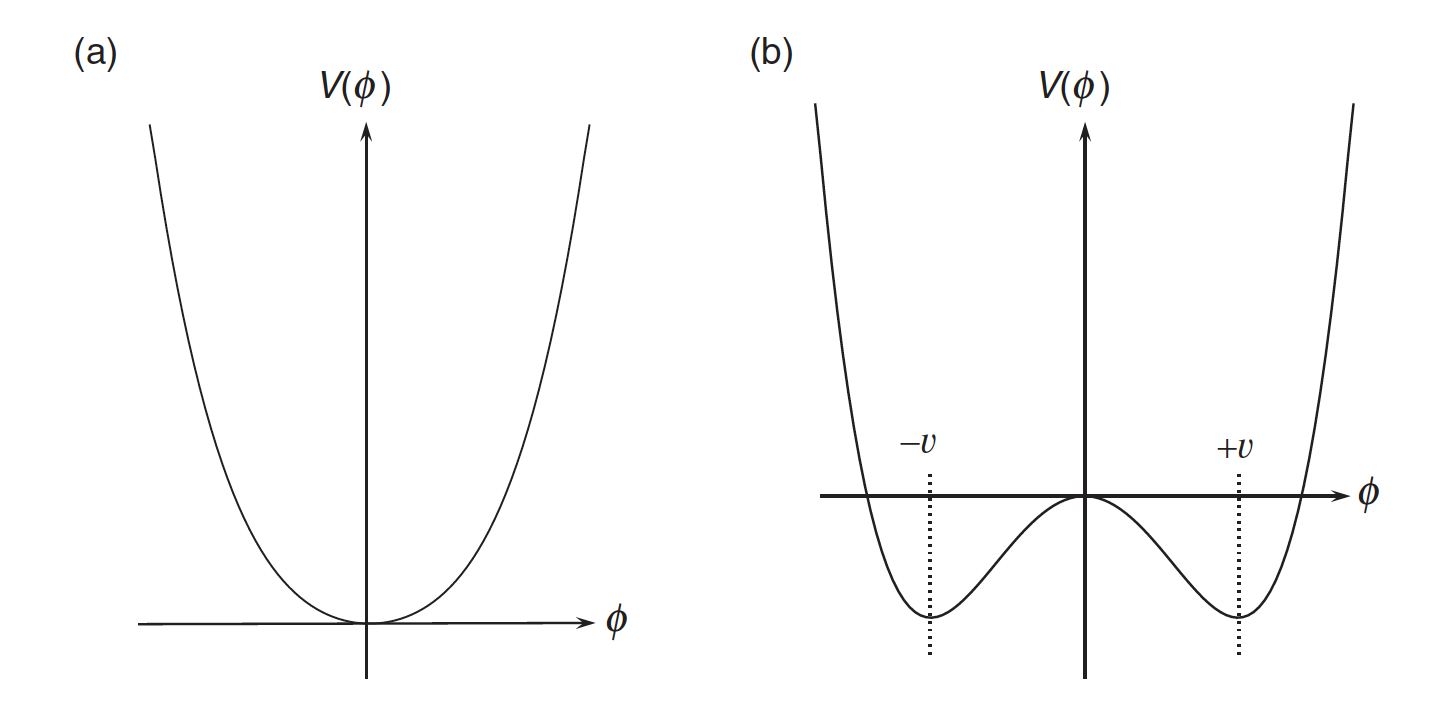
\includegraphics[width=0.55\textwidth]{Figures/c1/higgsPotential}
\caption{One dimensional representation~\cite{thomson_2013} of the Higgs potential in case (a) of $\mu^2 > 0$ and minimum for $\phi = 0$ for an unbroken theory and in case (b) for $\mu^2 < 0$ and VEV for a spontaneous symmetry breaking.}
\label{fig:mexico}
\end{figure}

Starting from Eq.~\ref{eq:higgsM}, it can be written $\phi^+=\nicefrac{(\phi_1 + i\phi_2)}{\sqrt{2}}$ and $\phi^0=\nicefrac{(\phi_3 + i\phi_4)}{\sqrt{2}}$ and knowing $2\phi^\dag \phi = \phi^2_1+\phi^2_2+ \phi^2_3+ \phi^2_4 = v^2$ it is clear that the minima form a four-dimensional sphere.\\
Furthermore, studying the region of the vacuum and choosing a particular vacuum in the $SU(2)$ space with $\phi_3 = v$ and $\phi_1=\phi_2=\phi_4=0$, it is possible to expand around the minimum and write:
\begin{equation}
\label{eq:higgsphi2}
\phi(x) = \frac{1}{\sqrt{2}}\begin{pmatrix}
0\\
v+ h^0
\end{pmatrix}
\end{equation}
where $h^0$ is a scalar Higgs field. Now combining and replacing~\ref{eq:SMderivative} and~\ref{eq:higgsphi2} into the Lagrangian~\ref{eq:higgsL} it happens that photon field remains massless while the two mass terms for \PW and \PZ bosons are naturally obtained:
\begin{align}
\left(\frac{vg_2}{2}\right) ^2W^{+\mu}W^-_{\mu} \; &\rightarrow \; m^2_W = \frac{g_2^2v^2}{4}\label{eq:massW}\\
\left(\frac{v\sqrt{g_1^2+g_2^2}}{2}\right)^2\frac{Z^{\mu}Z_{\mu}}{2} \; &\rightarrow \; m^2_Z = \frac{(g_1^2+g_2^2)v^2}{4}\label{eq:massZ}
\end{align}
Identifying those terms with the electroweak gauge-bosons allows for the extrapolation of the expectation value $v = \sqrt{\nicefrac{\mu^2}{\lambda}} = 246$\GeV of the Higgs field in the vacuum.
The three components $\phi_1,\phi_2$ and $\phi_4$ are referred to as massless Goldstone bosons and, as it was shown before, in a specific gauge choice called \emph{unitary gauge} ($\phi_3 = v$ and $\phi_1=\phi_2=\phi_4=0$) they do vanish. The remaining degree of freedom, the scalar field $h^0$, is known as Brout-Englert-Higgs boson. The mass of this SM Higgs boson is equal to $\sqrt{2\lambda}v$, with $\lambda$ being a free parameter in the SM, and
hence, there is no a priori prediction for the Higgs mass. The experimental measurements of the Higgs boson mass state  $m_{h^0}=125.10\pm0.14$\GeV~\cite{pdgw}. Finally, $h^0$ has no electric charge, and it has weak isospin $T_3=-1/2$ and hypercharge $Y=1$.

Once the mass problem of the \PW and \PZ bosons is fixed, it is necessary to address the problem of the generation of the mass terms for the SM fermions.
Introducing Yukawa interactions between fermions and the scalar field into the SM Lagrangian, the mass terms for SM fermions are fixed:
\begin{equation}
\label{eq:yukawa}
 \mathcal{L}_{\text{Yukawa}} \;\; = \;\; -\lambda^{ij}_dq^{-i}_L\phi d^j_R \;-\; \lambda^{ij}_uq^{-i}_L\tilde{\phi} u^j_R \;-\; \lambda^{ij}_{\ell}\overline{\ell}^{-i}_L\phi e^j_R \;+\; \text{hermitian conjugate}
\end{equation}
where $\tilde{\phi}= i\sigma\phi^*$, $q_L$ is a LH quark doublet, $u_R$ and $d_R$ are RH up and down quark singlets, $\ell_L$ is the LH doublet of leptons while $e_R$ is the RH lepton singlet. $\lambda^{ij}_u$, $\lambda^{ij}_d$ and $\lambda^{ij}_\ell$ are the up-quark, down-quark and lepton Yukawa coupling strengths ($i,j$ being the generation indices).

To conclude, while the boson mass term is determined by a gauge principle, the fermionic couplings with the Higgs field are not. Consequently, the corresponding Yukawa coupling constants (or the fermionic masses) are free parameters of the theory in contrast with the bosons masses which 
 are established by the couplings of the gauge interactions and the VEV of the Higgs field.


\clearpage

\section{Beyond the Standard Model}\label{sec:bsm}
The SM describes exceptionally well nearly all the processes that have been observed in particle physics, and its predictions do agree with an outstanding level of accuracy with the results from numerous precision measurements. Even though the theory has not shown any decisive evidence of where it can fail or where the formulation can be inaccurate, we know by now the SM does not cover the full picture and there are several indications that other fundamental physics remains to be unmasked.

In this section a few of the open questions in physics are very briefly listed and described trying to show why new physics beyond the SM is to be expected. Furthermore, some simplified explanations of such possible theories or extensions are provided. They will be discussed either the scenarios with additional particles and symmetries or the introduction of a more general theory for very high energies while considering the SM as an effective theory at current or lower energy scales.\\
Taking into account the context of this work, the focus will be heavily steered towards the introduction of RH heavy neutrinos as Beyond the SM theory and solution.



\subsection{Open questions of the Standard Model}\label{sec:questions}
\subsubsection{Gravity}
The Standard Model does not contain a description of gravitational interactions therefore being incomplete and failing to incorporate the general relativity theory in the SM theory itself. Proposals to describe gravity as a quantum field theory have included a possible spin-2 boson, called graviton, as mediator of the gravitational force; however, no experimental evidence have been found up to now. 

\subsubsection{Dark matter and dark energy}

It is well known today from several unquestionable cosmological observations that only roughly 5$\%$ of all the energy content of the universe consists of the baryonic matter as defined and included in the SM, then so-called \emph{ordinary matter}. In the standard $\Lambda$CDM model of cosmology, on top of the $\approx 5\%$ of ordinary matter, about 27\% is made up of another kind of matter that appears to be not directly visible (it does not interact with the electromagnetic field) and thus is so-called \emph{Dark Matter} (DM). The residual 68\% is called \emph{Dark Energy}. Hence DM is 85\% of the total mass and up to know we can fully describe and predict only 5\% of the universe. The values are obtained from observation of the CMB (cosmic microwave background) by the Planck satellite and published in this exhaustive review~\cite{2020Plank}.

There are several cosmological observational evidence for dark matter. We can cite the calculations of the velocity dispersion and the rotation curves of galaxies, the gravitational lensing measurements and the distribution of the cosmic microwave background; additionally there are the astronomical observations of the universe's current structure and the formation and evolution of structures as galaxies and nebulas.\\
\begin{figure}[h]
\centering
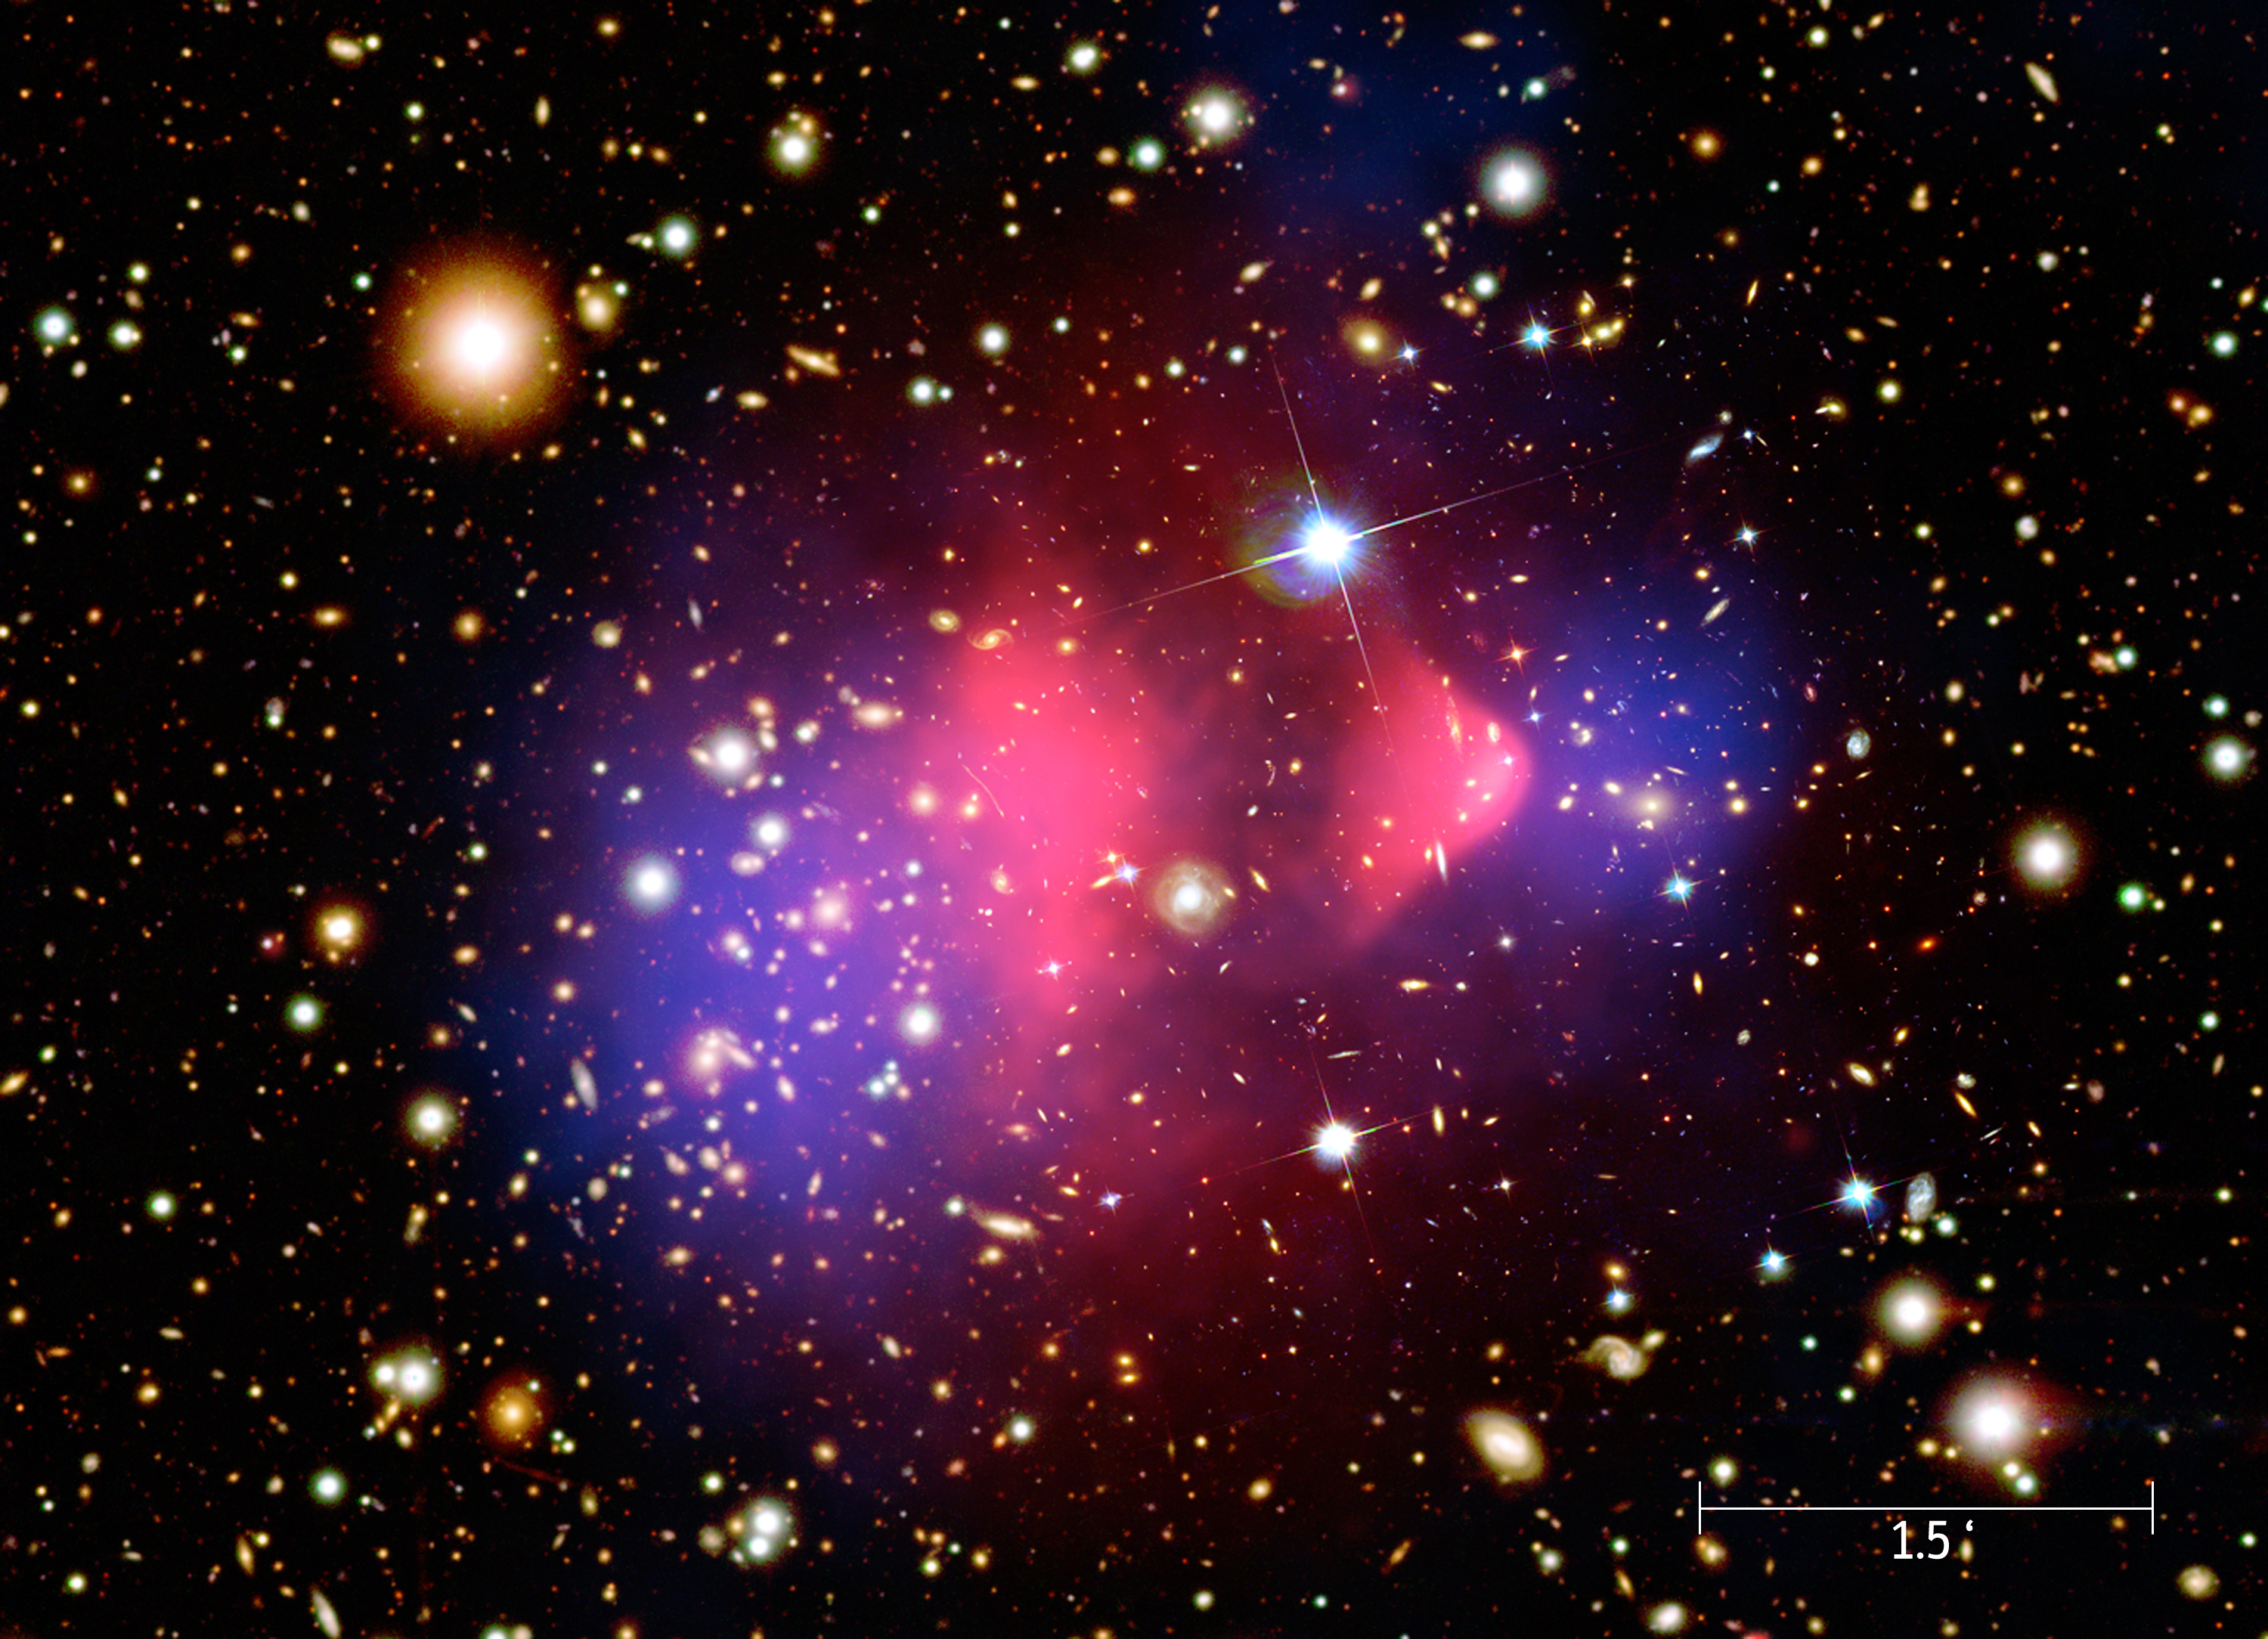
\includegraphics[width=0.65\textwidth]{Figures/c1/bullet.jpg}
\caption{X-ray image (pink) superimposed over a visible light imagine (galaxies) with the matter distribution (DM plus ordinary matter) calculated from gravitational lensing (blue)~\cite{webpage_bullet}}
\label{fig:bullet}
\end{figure}
An interesting and very clear example is the one coming from the observation of the \emph{Bullet Cluster} (1E 0657-56)~\cite{Clowe_2004} (see Fig.~\ref{fig:bullet}) which is a transparent proof of DM. The \emph{Bullet Cluster} indicates a smaller sub-cluster (on the right in Fig.~\ref{fig:bullet}) moving away from a larger one in a bigger structure consisting of two colliding clusters of galaxies. Comparing the information obtained through X-rays measurements, which quantify the hot gas of baryonic matter, with the total amount of matter (DM plus ordinary matter) detected indirectly by the gravitational lensing of background objects, the Bullet Cluster provides 
one of the best evidence to date for the existence of dark matter. With a statistical significance of 8$\sigma$ it was addressed that ``spatial offset of the center of the total mass from the center of the baryonic mass peaks cannot be explained with an alteration of the gravitational force law alone, and thus proves that the majority of the matter in the system is unseen''~\cite{Clowe_2006}.

All cosmological evidence of DM relies on its gravitational effects, which is the only type of interaction that, up to now, DM is expected to have with ordinary matter.\\
Since it is still unknown which is the nature of DM, dark matter searches are one of the hottest and most fascinating  topics in both particle physics and theoretical physics. Several experiments have tried to detect DM through either direct detection or indirect detection and via collider experiments where the DM candidate could be produced in the collision of leptonic or hadronic beams. For clear reviews of DM searches at the CMS Experiment see~\cite{LOWETTE2016503,Bhawna_Gomber}.

Many candidates for DM have been sifted, some being part of more structured theories like Supersymmetry or others being completely new exotic particles. To give a simple list of possible solutions, candidates for non-baryonic dark matter could be particles like axions, weakly interacting massive particles (WIMPs),  gravitationally-interacting massive particles (GIMPs), supersymmetric particles and sterile neutrinos. The latter are very interesting in the scenario of this thesis work too, providing an excellent aspirant as DM~\cite{DREWES2017250,Cline_2020}. Sterile neutrinos (or neutral leptons) are defined to interact only via gravity and do not couple with any gauge fields of the SM, hence the name \emph{sterile} to distinguish them from the \emph{active} neutrinos of the SM. In the following references a few interesting models with sterile neutrinos as DM candidate are listed~\cite{Davidson_2008,PhysRevLett.72.17,PhysRevD.64.023501,KUSENKO20091,DOLGOV2002339}.


\subsubsection{Baryon asymmetry and CP violation}
The baryon asymmetry problem is also known as the matter-antimatter asymmetry problem and outlines the imbalance between the baryonic matter and the anti-baryonic matter in the observable universe.\\
 At the Big Bang instant, it is believed the same amount of matter and antimatter was produced, but the clear disproportion we observe today and in the early universe suggests that some physical laws must have operated differently for matter and antimatter. As proposed in 1967 by Andrei Sakharov~\cite{Sakharov:1967dj}, this matter-antimatter asymmetry can only be justified if the theory allows for a violation of charge-conjugation symmetry and of parity symmetry\footnote{Parity transformation is the inversion of the sign of one of the spatial coordinates; P-symmetry refers to equations and processes with are invariant under mirror inversions. All the interactions of elementary particles but weak interaction are symmetric under parity.}; these simultaneous violations are so-called CP violation. \\
The first observation of indirect CP violation was provided in 1964 by James Cronin and by Val Fitch with the ``the Fitch-Cronin Experiment''~\cite{PhysRevLett.13.138} where clear evidence was found of CP violation in neutral kaons decays.\\
For a direct CP violation proof, we needed to wait till 1999 for the results from KTeV experiment~\cite{Alavi_Harati_1999} at Fermilab and the observation from the NA48 experiment~\cite{Fanti_1999} at CERN. The most recent updates come from the LHCb experiment which has announced the discovery of CP violation in neutral D meson decay~\cite{PhysRevLett.122.211803}.

The sterile neutrinos, previously mentioned, are seen as possible candidates to address the matter-antimatter asymmetry problem thanks to their different behaviors under CP transformation with respect to Dirac neutrinos. In the following references~\cite{Gandhi_2015,Klop_2015,Palazzo_2020}  there are a few examples of experimental results interpretations with the sterile neutrinos in the context of CP violation theories.

\subsubsection{Neutrino masses}
In Eq.~\ref{eq:yukawa}, the Yukawa Lagrangian, it is clear the absence of the mass term for the neutrinos. As mentioned and explained in Sec~\ref{sec:ewk} (Eq.~\ref{eq:LR2}), it is in principle possible to add the mass term as a RH component in the Lagrangian. Nevertheless, up to this day, the RH neutrinos have not been found and it is expected to be very difficult to observe them knowing that the RH fermions do transform as singlets under the entire SM gauge group and consequently they are sterile. It was then accepted for a long time that the neutrinos would be massless particles in the SM.

The whole understanding of the SM neutrino was shaken and weakened in 1968 with the results from the Brookhaven National Laboratory obtained with the Brookhaven solar neutrino detector~\cite{PhysRevLett.20.1205}.
It was obeserved that the number of neutrinos coming from the sun was significantly lower with respect to the expected value using solar-model calculations of the neutrino flux from decay of ${}^{8}B$\footnote{For the experiment at the Brookhaven National Laboratory, the calculations of the flux of solar neutrino coming from boron-8 decay were used: ${}^{8}B\rightarrow {}^{8}Be + e^{+} + \nu_e$. For a simple scheme and explanation see webpage~\cite{webpage_boron}.} inside the sun. This was the first hint of the so-called \emph{solar neutrino problem}.\\
The explanation for this deficiency and for the other observed ``neutrino anomalies'' during those years was found to be the existence of neutrino flavor oscillations, theoretically predicted in 1957 by Bruno Pontecorvo~\cite{osti_4343073}. \\
The first crucial evidence for these speculations arrived in 1998 with the results from Super-Kamiokande Observatory~\cite{Fukuda_1998}. The data showed a angularly dependent deficit of $\nu_{\mu}$ which is not consistent with the expectations based on the calculation of the atmospheric neutrino flux. The difference in angular distribution between neutrinos coming from above the detector and the one coming from below (going through the earth) suggested a higher survival probability for $\nu_{\mu}$ traveling a shorter distance.\\
The first direct observation of the oscillation of the electron neutrino to other flavors was only in 2001~\cite{Ahmad_2001} at the Sudbury Neutrino Observatory in Canada. The experiment was designed to detect solar neutrinos from the decay of ${}^{8}B$ via the charged current (CC) reaction on ${}^{2}H$ and by elastic scattering (ES) of electrons; the first reaction (CC) was sensitive only to $\nu_e$, while the ES reaction also to  $\nu_{\mu}$ and $\nu_{\tau}$. Starting from the assumption that the fusion processes in the sun produce only electron neutrinos, a flux of $\nu_{e}$ equal to the one calculated from ${}^{8}B$  decays was expected. The total flux of electron neutrino was instead found to be much lower than the predictions (as for~\cite{PhysRevLett.20.1205}) but the total rate, $\nu_{e} + \nu_{\mu} + \nu_{\tau}$ was surprisingly in line with the number of neutrinos expected to arrive from the sun. This was the first direct evidence of the flavor neutrino oscillation, \ie neutrinos change flavor when traveling long distances. The phenomenon in which a neutrino can be created with a specific lepton number and then, after being propagated through space, can be measured to have a different lepton number, is called neutrino oscillation and it can happen only if the neutrinos have a non-zero mass. Then, the main question would be how the neutrino masses arise.

One of the most promising explanations is the addition of the Majorana mass term in Eq.~\ref{eq:yukawa}. This theory, which is the main topic of this thesis, is going to be extensively explored in Chapter~\ref{Chapter3}.


\section{Summary}\label{sec:summaryC1}
Everything is solved by sterile neutrinos!!!! Viva HNLs!!!






% Chapter Template
\chapter{!!NOT DONE!! The CMS experiment at the LHC !!NOT DONE!!} \label{Chapter2} 



This chapter outlines the main characteristics of the Large
Hadron Collider (LHC) in Section~\ref{lhc} and of the Compact Muon Solenoid (CMS)
detector in Section~\ref{cms}. In Section~\ref{sec:reconstruction}, it is
given an explanation of the reconstruction algorithm, called
\emph{Particle flow}, and reconstruction performances are
discussed. The main focus of Sections~\ref{cms}
and~\ref{sec:reconstruction} will be on lepton (electrons and muons) identification and
reconstruction in consideration of the multilepton final states which are
discussed in Chapter~\ref{Chapter5} and~\ref{Chapter6} and thus are
central to this dissertation.



%----------------------------------------------------------------------------------------
%	SECTION 1
%----------------------------------------------------------------------------------------
\section{The Large Hadron Collider}\label{lhc}

The LHC~\cite{Brning2004LHCDR} is a circular particle accelerator
located at the CERN laboratories in Geneva operating since 10
September 2008. It is
designed to accelerate hadrons (like protons, Lead-ions, Xenon-ions) and to
operate at the centre-of-mass energy of 14\TeV.
The circular ring is installed in a tunnel of a 27 kilometers where
the Large Electron Positron collider~\cite{Lep:designReport} was
previously located.\\
A graphic representation of CERN accelerator
complex is shown in Figure~\ref{fig:cern} where the particle
accelerations begins at the LINAC, foregoing booster, PS and SPS, in
order. The LHC consists of accelerating components as well as
superconducting magnets to focus the hadrons, keep them on the right
trajectory and squeeze them tight together right before the
collision point. 

\begin{figure}[h]
\centering
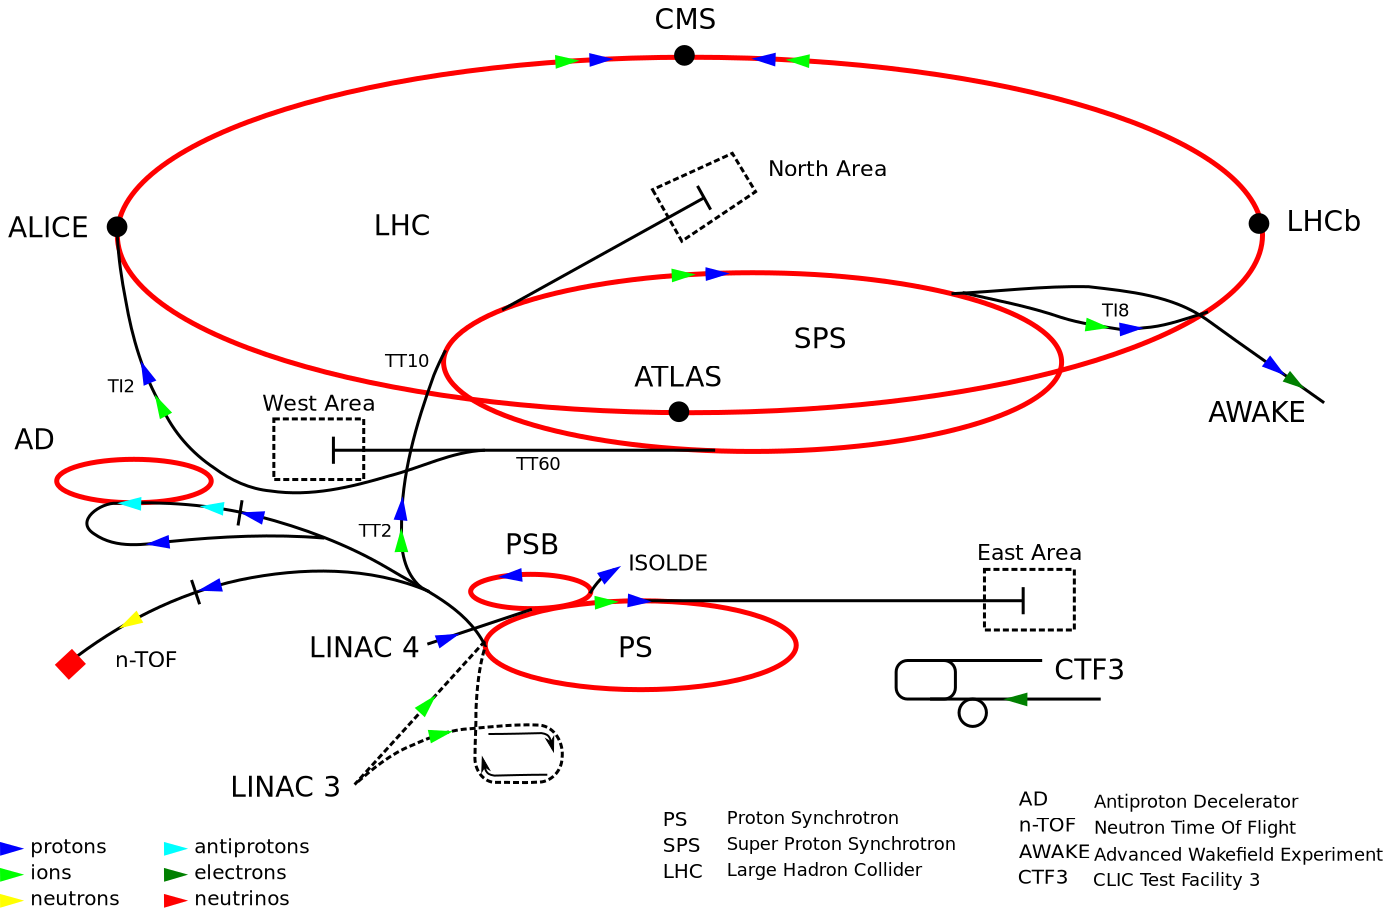
\includegraphics[width=0.75\textwidth]{Figures/c2/Cern-accelerator-complex.png}
\vspace*{3mm}
\caption{The LHC is the largest ring (top) in a complex chain of particle accelerators. The smaller machines are used in a chain to help boost the particles to their final energies and provide beams to a whole set of smaller experiments, which also aim to uncover the mysteries of the Universe~\cite{Mobs:2197559}}
\label{fig:cern}
\end{figure}

The protons are accelerated in opposite directions in two distinct
accelerator tubes which cross at four interactions points where the
protons are made to collide. At each of the interaction points along the ring,
four experiments are located with the aim to reconstruct the
sub-atomic particles which are made at the moment of a high energy
collision. The protons are grouped in bunches which are
accelerated in steps using the full accelerator chain consisting in a linear
accelerator, boosters, synchrotrons and, at the end, they are injected
into the LHC with an energy of 540\GeV where a system of
superconducting magnets further accelerate them up to 13\TeV. Every
25 ns collisions between proton bunches occur meaning 40 million
bunch crossing per second. At full regime during data taking time
period about 2800 bunches travel in the LHC rings and each bunch is
made of up to $1.1\times10^{11}$ protons.

The four experiments located at the four interaction points are
ALICE~\cite{alice_2008} (A Large Ion Collider Experiment),
ATLAS~\cite{atlas_2008} (A Toroidal LHC ApparatuS),
CMS~\cite{cms_2008} and LHCb~\cite{lhcb_2008} (Large Hadron Collider
beauty), refer to Figure~\ref{fig:cern}. ALICE experiment is designed
to study the presence and the properties of the hypothetical
quark-gluon plasma formed during heavy ions collisions, LHCb is
designed to be very sensitive in analyzing the properties of the B
mesons. The last two, ATLAS and CMS are general purpose detectors
designed to investigate a vast range of physics scenarios starting
from the search and discovery of the Higgs boson to extra dimensions
and dark matter. \\

The accelerator-dependent features and parameters which are important for a
physics analysis are the instantaneous and integrated luminosity, the
number, in the same bunch crossing, of simultaneous collisions and the
center-of-mass energy of the proton-proton collisions.

The instantaneous luminosity is defined as a time dependent
parameter, $d\mathcal{L}/dt$, which correlates the number of collisions
($N$) in a certain amount of time ($t$) and the cross section of a
given process through the relation:
\begin{equation}
\label{eq:instalumi}
\frac{dN}{dt} \: = \: \frac{d\mathcal{L}}{dt}\sigma
\end{equation}

The unit of the instantaneous luminosity is $b^{-1}s^{-1}$, where 1
barn $= 10^{-24} \ cm^2$ and it depends on the number of bunches in
the proton beam, on the number of protons per bunch and on the beam
optics. \\
The integrated luminosity is the integral of the instantaneous
luminosity over time, and relates the cross section of a
given process to the number of events $N$ of that process:
\begin{equation}
\label{eq:intelumi}
\mathcal{L} \:=\: \int \frac{d\mathcal{L}}{dt} dt \: = \: \frac{N}{\sigma}
\end{equation}


\begin{figure}[h]
  \noindent
  \makebox[\textwidth]{
  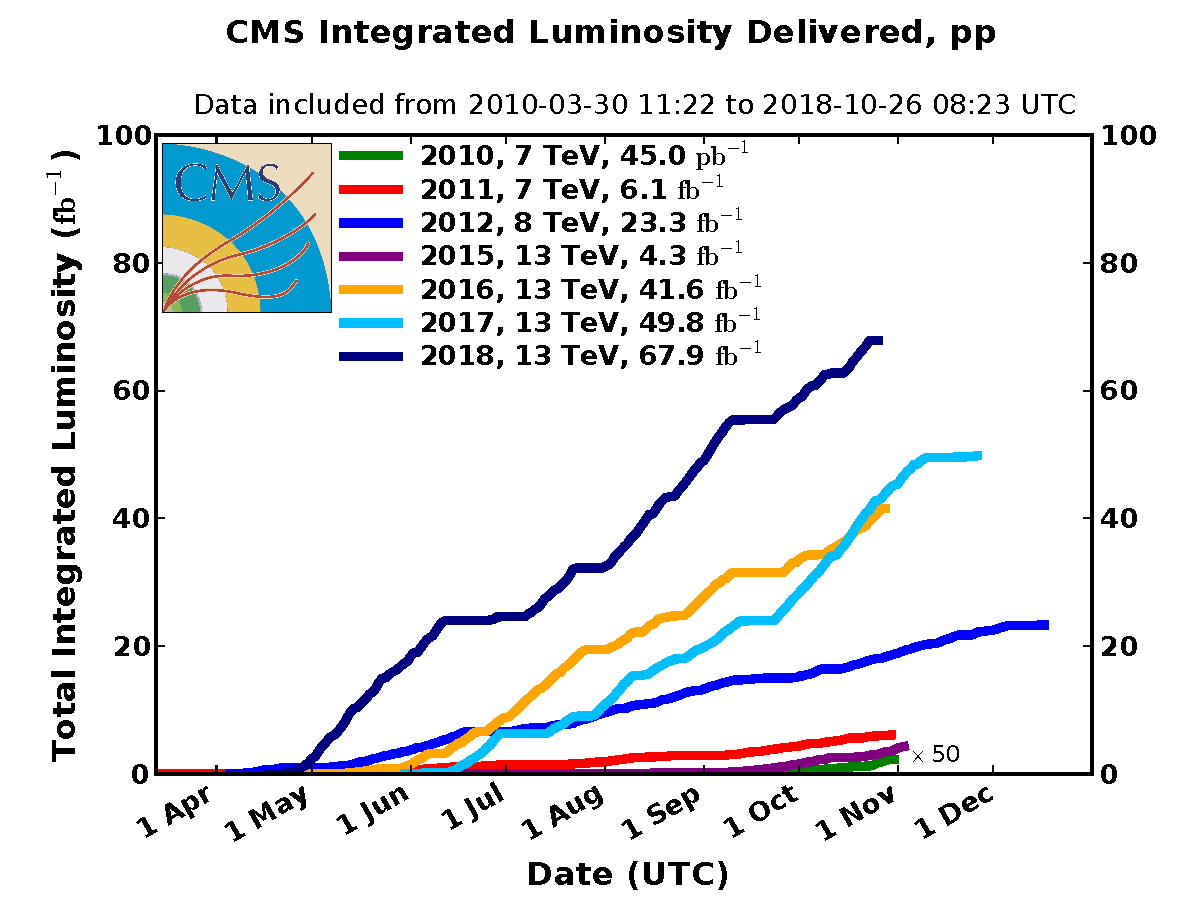
\includegraphics[width=.50\textwidth]{Figures/c2/int_lumi_cumulative_pp_2.pdf}
  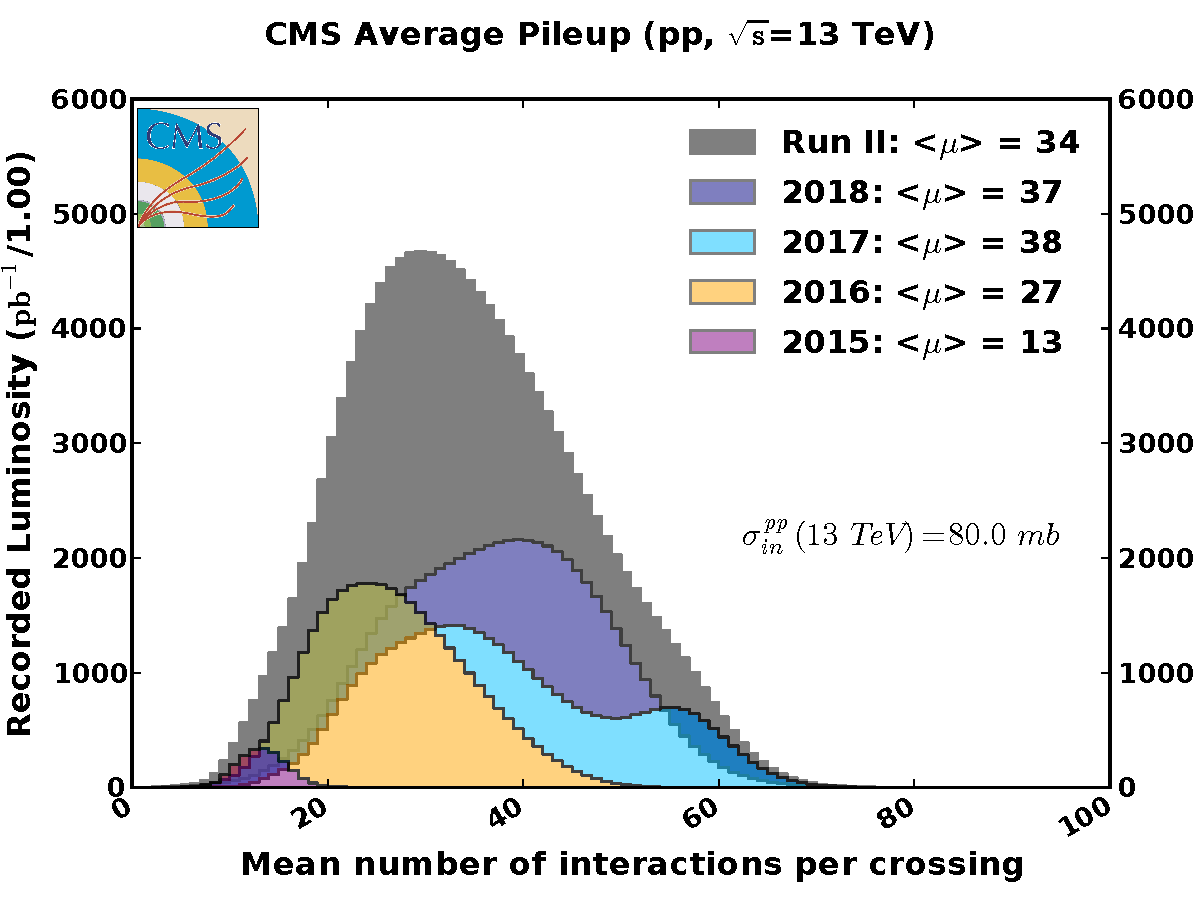
\includegraphics[width=.50\textwidth]{Figures/c2/pileup_allYears_run2.pdf}}\\
  \makebox[\textwidth]{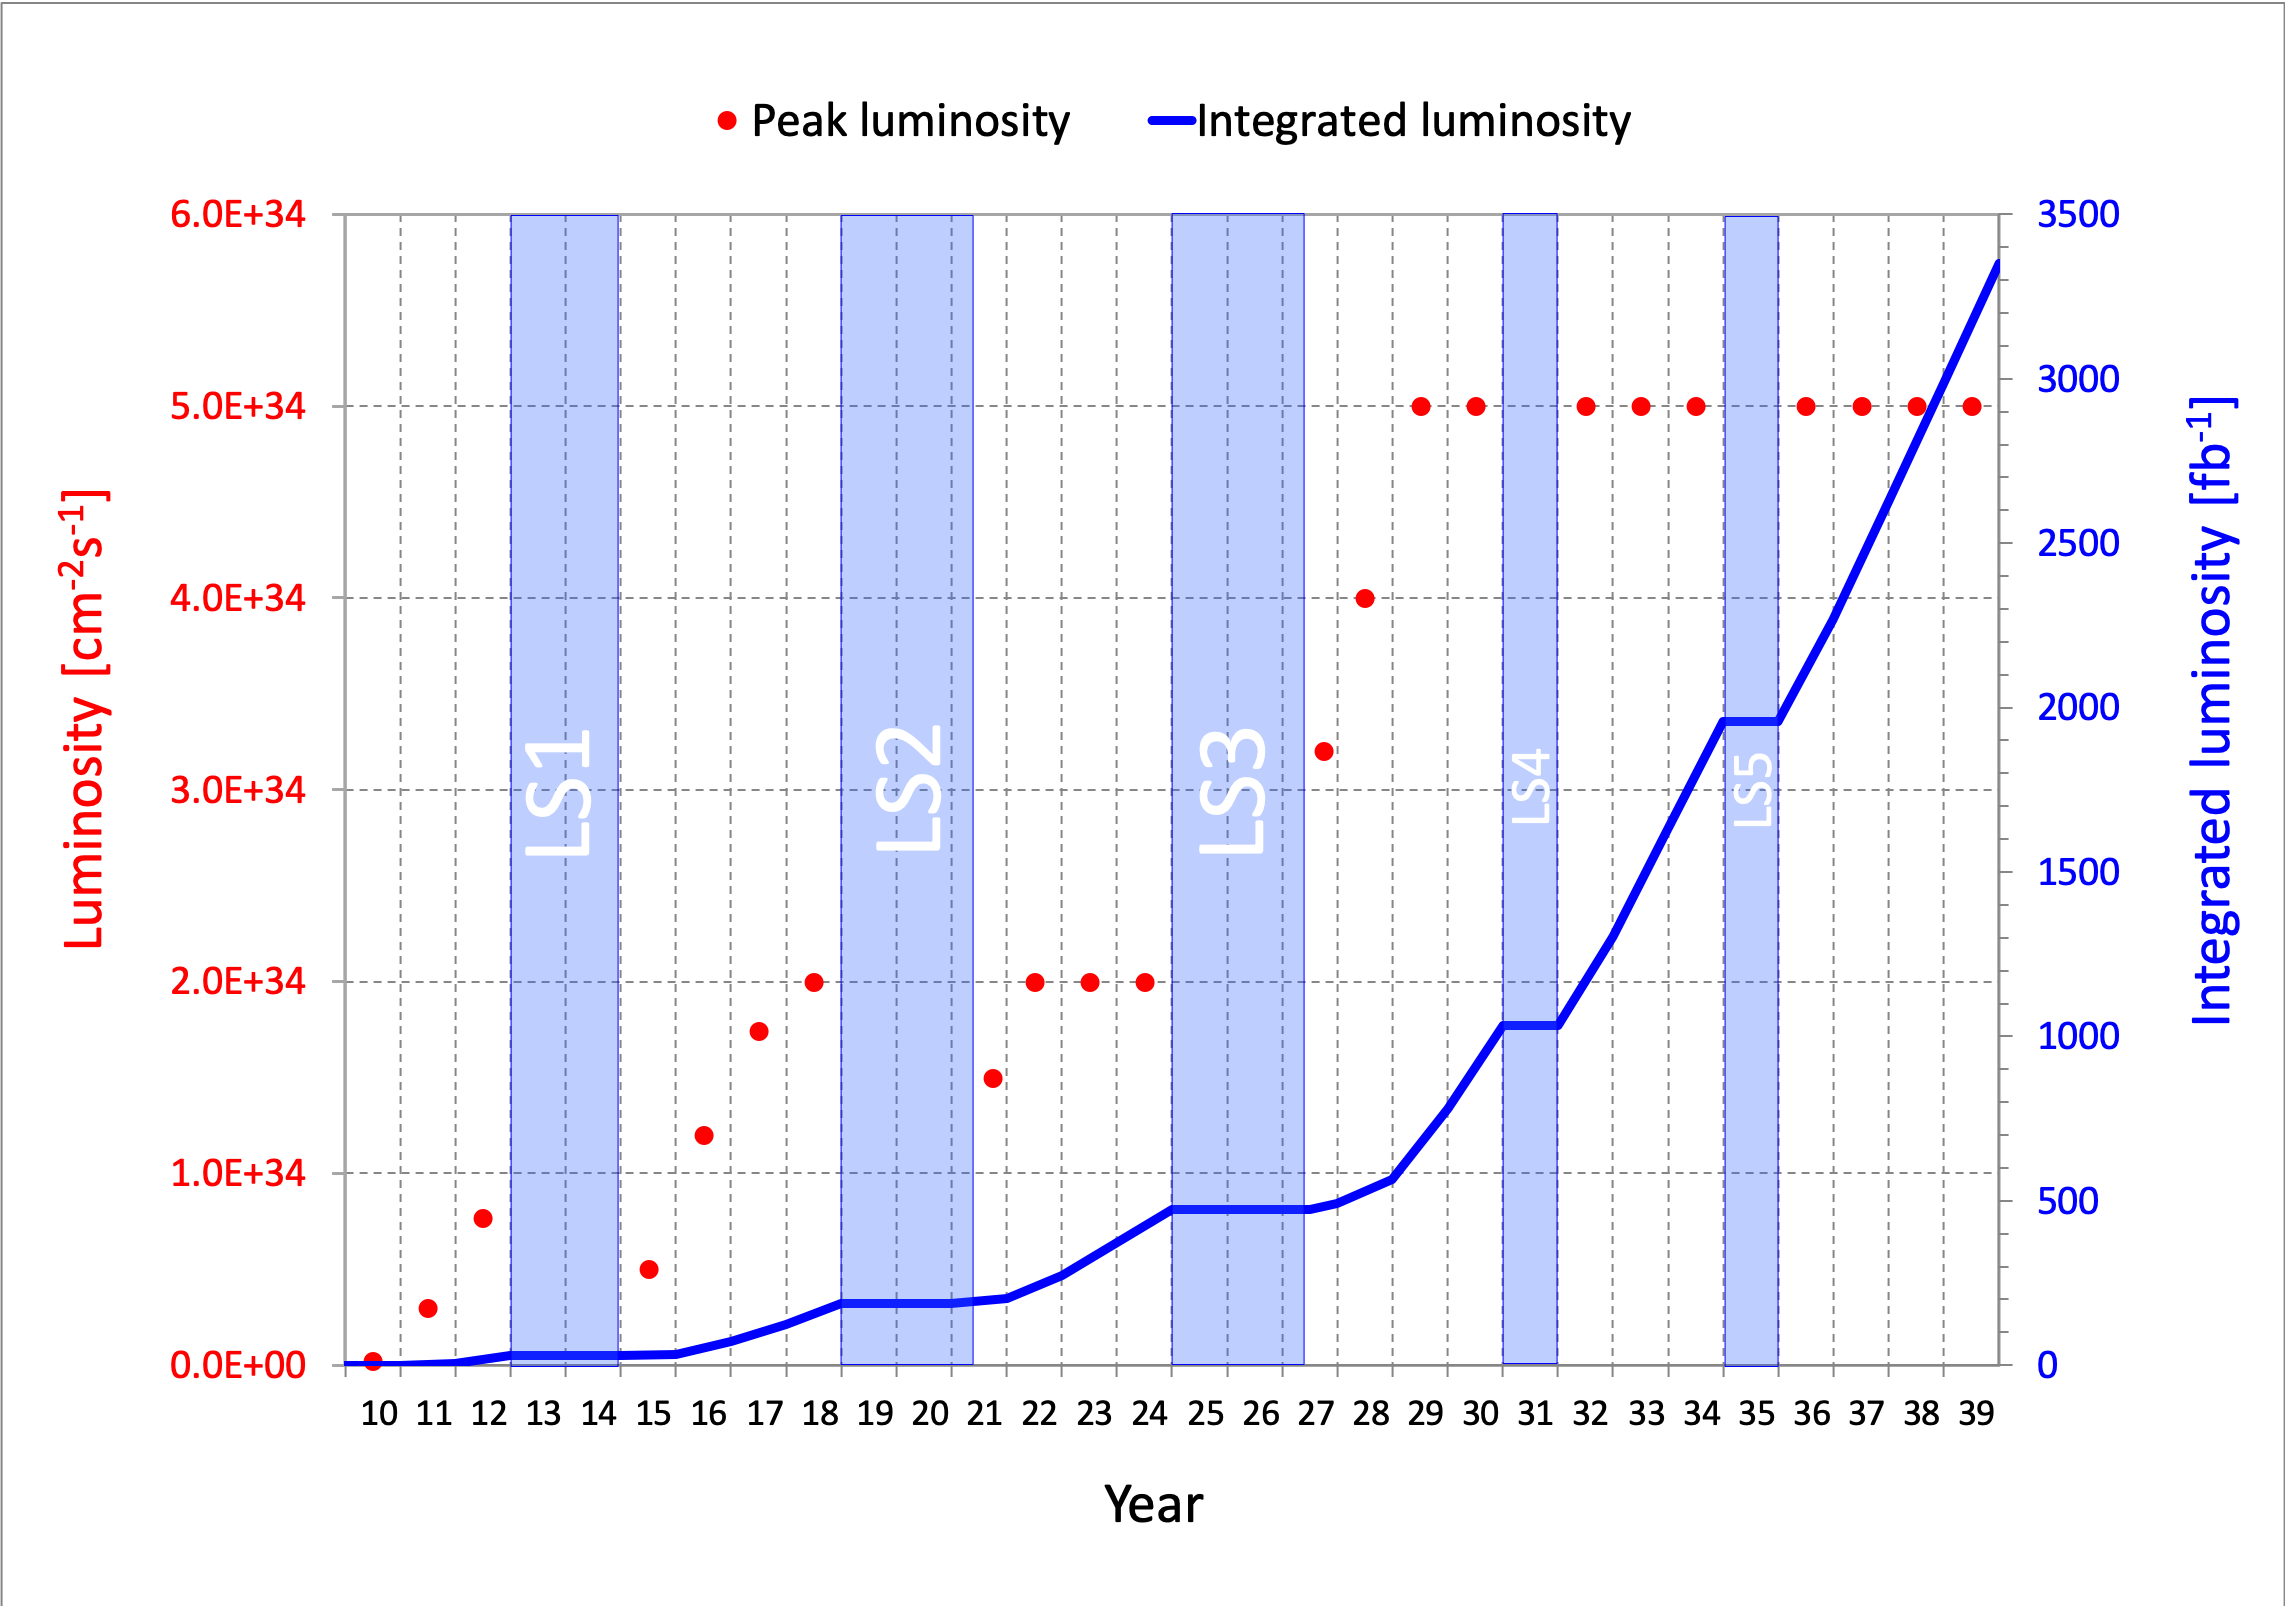
\includegraphics[clip,trim=0.2cm 0.2cm 0.2cm 0.2cm, width=.60\textwidth]{Figures/c2/Lumi.png}}
  \caption{Top-left: integrated luminosity collected by the CMS
    experiment; top-right: distribution of the average number of
    interactions per crossing (pileup) for pp collisions in 2015
    (purple), 2016 (yellow), 2017 (azure), 2018 (periwinkle), and
    full Run2 (gray),~\cite{webpage_lumi}. Bottom: scheduled and
    projected integrated and instantaneous luminosity at the LHC~\cite{webpage_lhc}.}
  \label{fig:lumi}
\end{figure}

The LHC was designed to deliver an instantaneous luminosity
of $10^{34}cm^{-2}s^{-1}$. Figure~\ref{fig:lumi} (top-left and central
plots) shows the schedule of the Large Hadron Collider from the start
to the following years of operations. The LHC has delivered two
outstanding runs of data taking: the first phase, Run1 (2010-2012) at
center-of-mass energy of 7 and 8\TeV and total delivered integrated
luminosity of $29.4\ fb^{-1}$; the first 3 years of data taking proved
the physics potentiality of the LHC with, among others, the Higgs boson
discovery. The second run, Run2 (2015-2018) started after 2 years Long
Shutdown when the machine and the detectors were confirmed and
consolidate to be able to run at the full capacity with 
center-of-mass energy of 13\TeV and total delivered integrated
luminosity of $162.9\ fb^{-1}$.\\
The increase in luminosity over the
years was the result of improvements in the beam quality and optics which
led to an higher number of pp collisions per bunch crossing. This
quantity is referred as pileup, PU which is shown in the top-right plot
in Figure~\ref{fig:lumi}. The average \textlangle{}PU\textrangle{} for
Run2 is 34. On one hand this large
number of collision per bunch crossing 
expands the physics reach of CMS and ATLAS because of
the higher probability of an episode of a rare collision; however
most of the PU interactions pollute the information of the
event being mostly soft and less interesting to look for
new physics models. Thus it is challenging for the detector and the for
the reconstruction algorithms to be able 
to disentangle and reconstruct each single pp collision per single
bunch crossing.

%-----------------------------------
%	SECTION 2
%-----------------------------------
\section{The Compact Muon Solenoid}\label{cms}

The Compact Muon Solenoid (CMS) detector is located at one of the four
collision points along the LHC ring, precisely at LHC P5 in Cessy in
France.  

CMS is a multi-purpose detector designed to observe any new physics
phenomena that could appear at proton-proton collision. CMS behaves
like a high-speed camera capturing instant frames of the particle
collisions up to 40 million times per second. Then by trying to
identify the particles produced and created after the collision,
measuring their energies and momenta the detector aims to recreate a
photograph of the collision for offline analysis. \\
The idea behind the design was to create, around the place where the
two proton beams cross each-other, a structure of concentric cylindrical layers
in order to be able to track and measure the path of the particle
escaping from the center.   

\subsection{The CMS coordinate system} 
The coordinate system used by CMS is a right-handed system defined
locating its center in
\begin{wrapfigure}{r}{0.5\textwidth}
  \begin{center}
    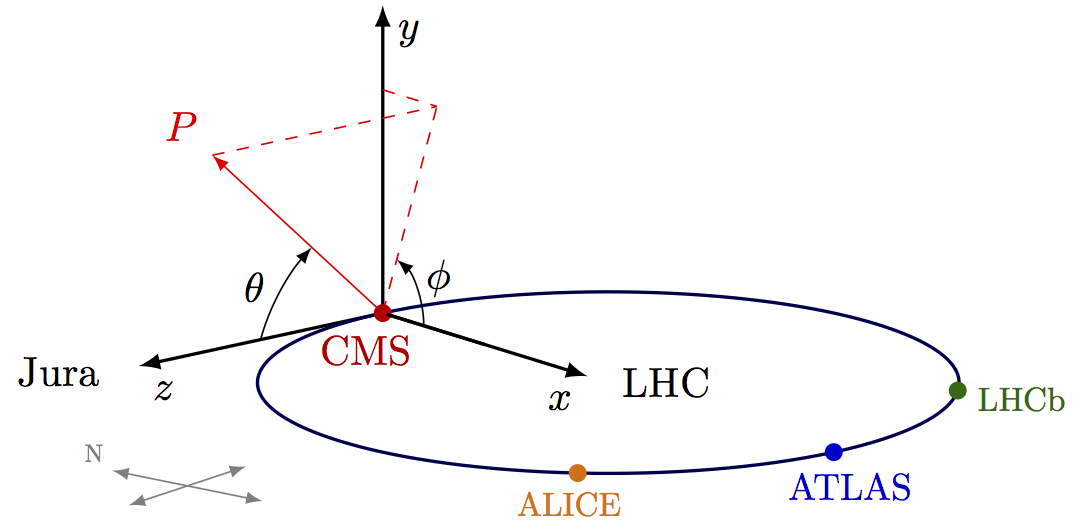
\includegraphics[clip,trim=0cm 0cm 0cm 0.1cm, width=0.48\textwidth]{Figures/c2/cms_coordinate_system.png}
  \end{center}
  \caption{A scheme of the coordinates system used by CMS~\cite{coordinate_cms}.}
\label{fig:coordinates}
\end{wrapfigure}
 the nominal interaction point, the
\emph{y}-axis is vertical pointing upwards, the \emph{x}-axis is
radial pointing inward towards the center of the LHC ring and the
\emph{z}-axis coincides with the direction of the beam
(counter-clockwise beam); refer to
Figure~\ref{fig:coordinates}. The azimuthal angle $\phi$ is defined
from the \emph{x}-axis in the \emph{x-y} plane and the polar angle
$\theta$ is measured from the \emph{z}-axis in the same transverse
plane meaning \emph{x-y} plane.\\
For an object of energy $E$ and momentum $\overrightarrow{p}$,
rapidity, $y$ and pseudorapidity, $\eta$ are defined as:
\begin{equation}
\label{eq:pseudo}
y \: = \: \frac{1}{2} \ln \frac{E + p_z}{E - p_z} \;\; \approx \;\;
\eta \: = \: \frac{1}{2} \ln \frac{|\overrightarrow{p}| +
  p_z}{|\overrightarrow{p}| - p_z} \: = \: -\ln \tan (\frac{\theta}{2})
\end{equation}
The approximation of the rapidity with the pseudorapity is possible for
relativistic particles with $p_{T} \gg m$. The rapidity is used to
measured the angular distance between particles, $\Delta R =
\sqrt{\Delta y ^2 + \Delta \phi ^2}$ which is Lorentz invariant under
boots along $z$-axis the beam direction. Knowing the approximation above,
the $\Delta R$ quantity is often defined as $\Delta R =
\sqrt{\Delta \eta ^2 + \Delta \phi ^2}$.\\
Finally, using the $x$ and $y$ components, the transverse variables
are defined: the transverse momentum, $p_T$ and the transverse energy,
$E_T$.


\subsection{CMS detector}\label{sec:cmsdetector}
The schematic representation of the CMS detector and its parts is
shown in Figure~\ref{fig:detector}.
\begin{figure}[h]
\centering
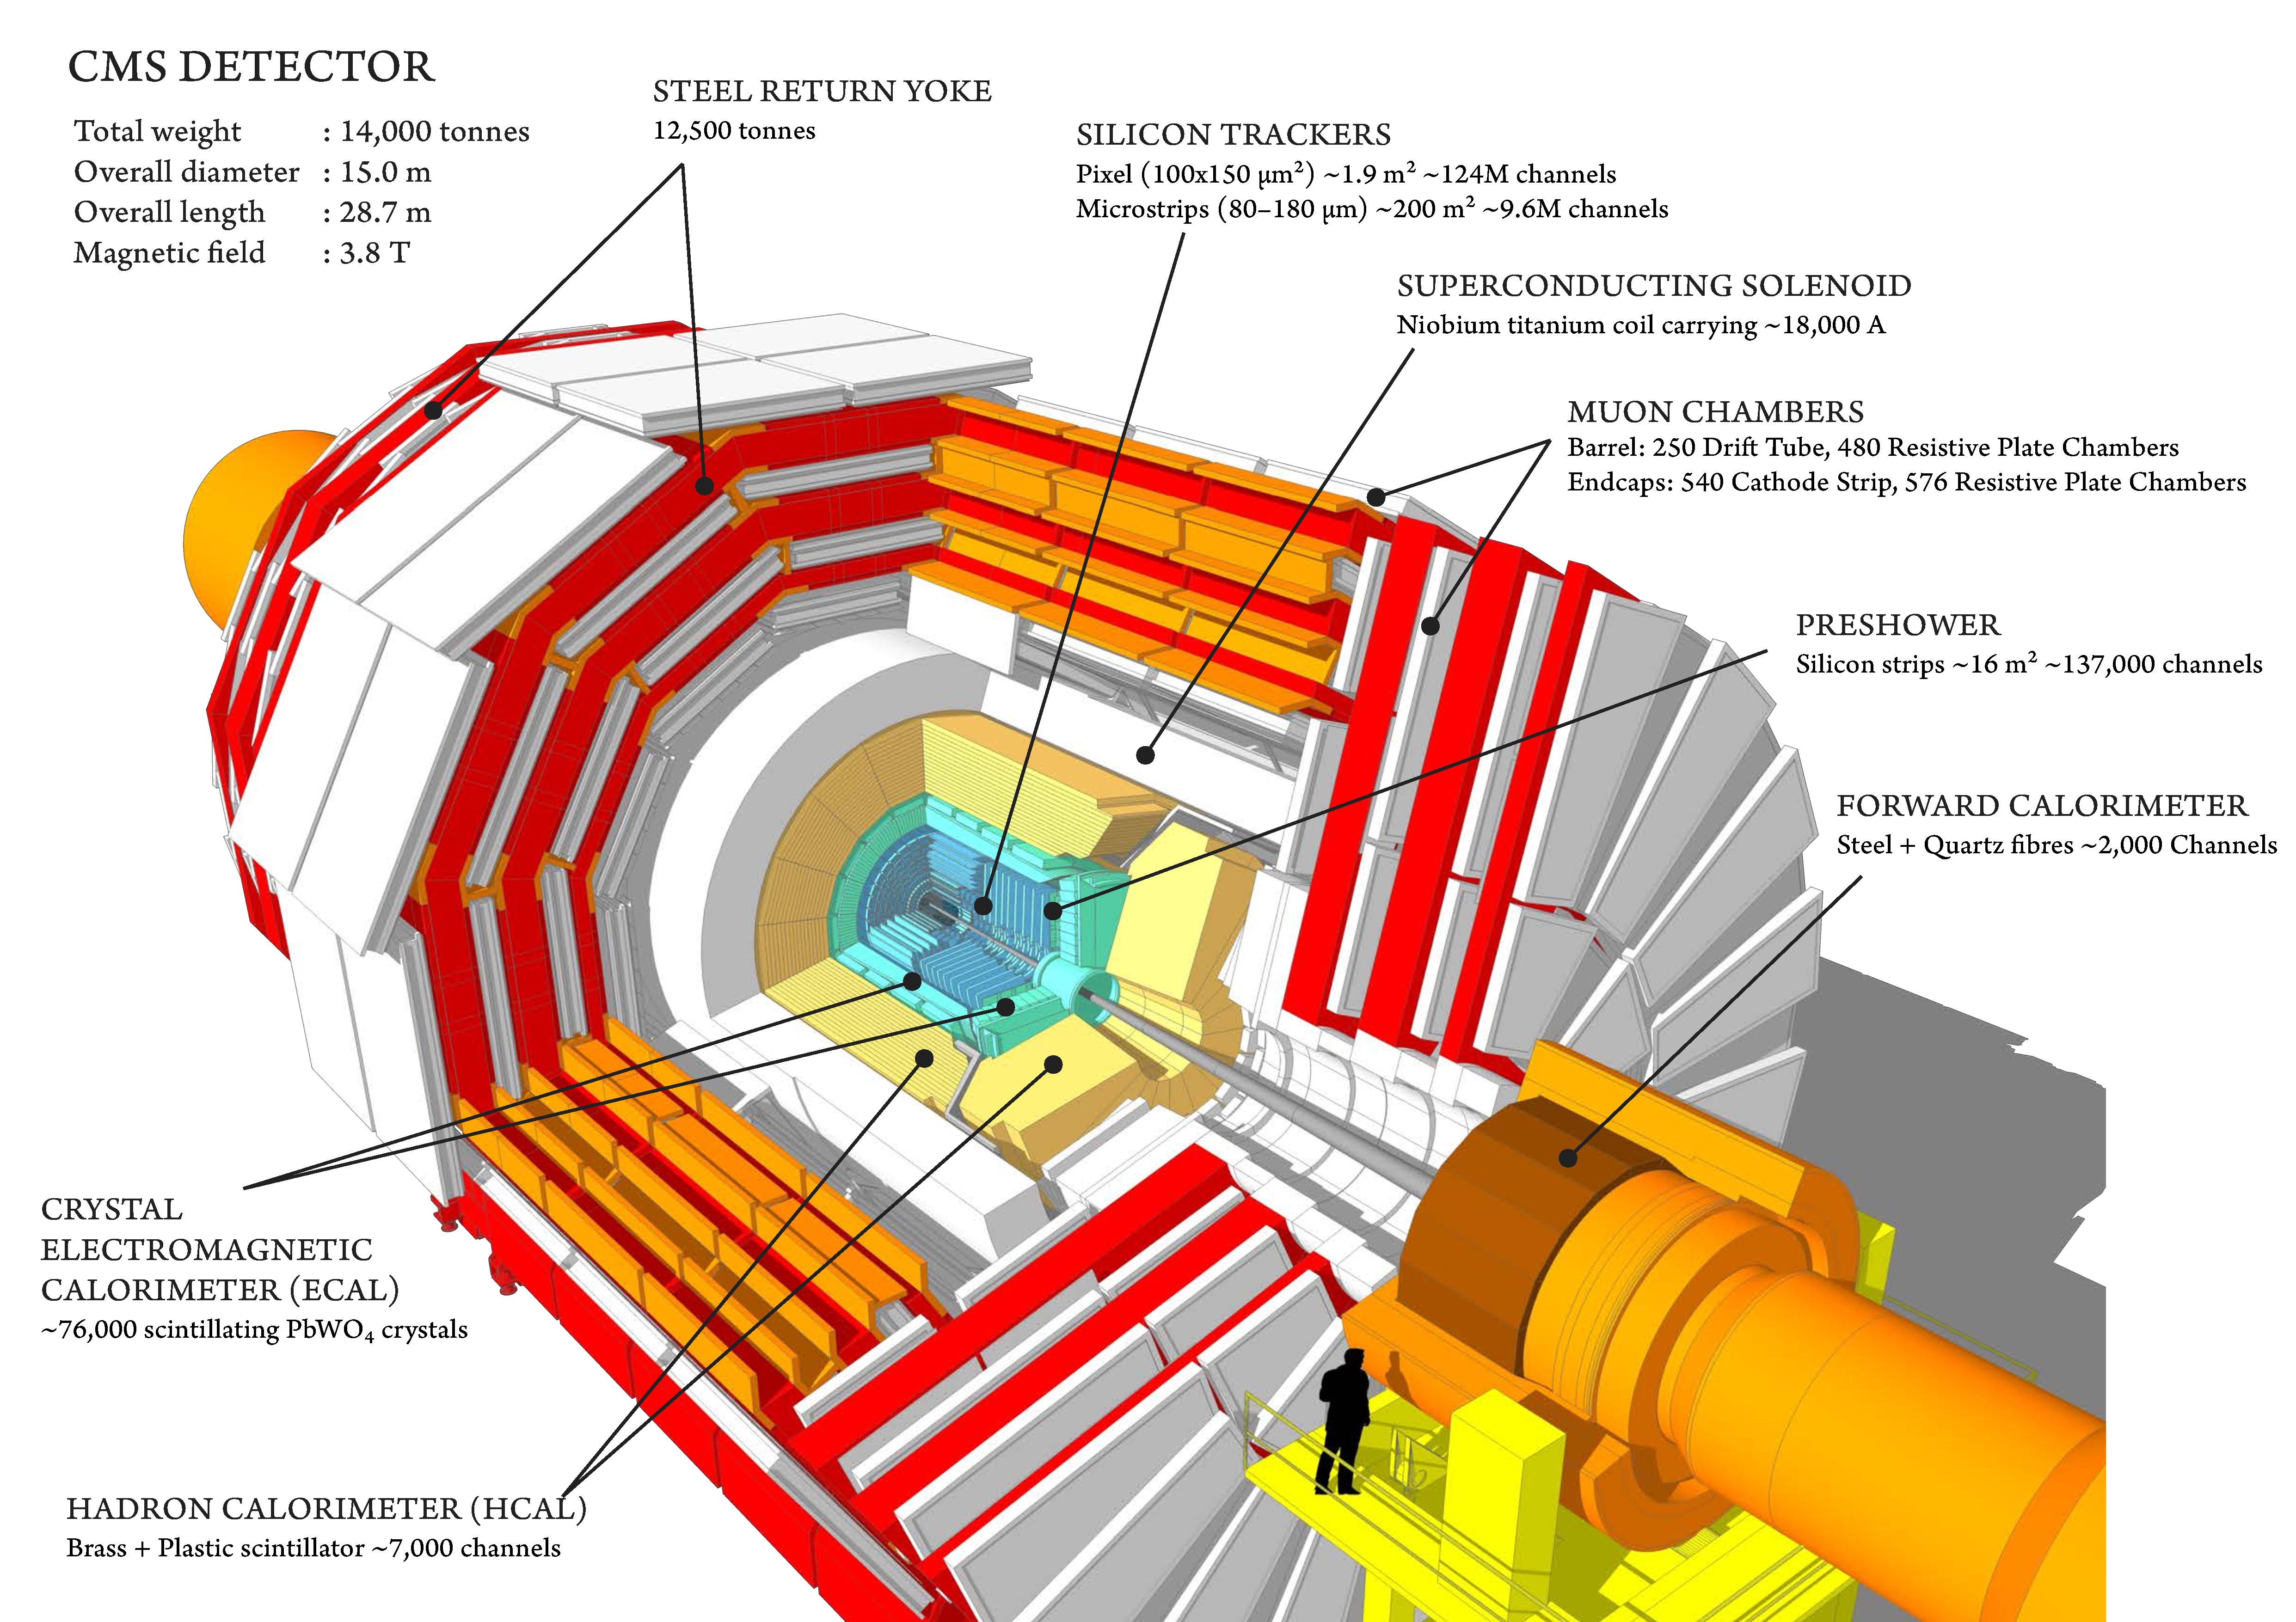
\includegraphics[width=0.98\textwidth]{Figures/c2/cms_160312_06-compressed.pdf}
\vspace*{3mm}
\caption{A scheme of the CMS detector and its parts~\cite{webpage_cms}.}
\label{fig:detector}
\end{figure} 

With CMS detector is possible to measure photons, electrons, muons and hadrons (neutral and charged). 
To be able to achieve such results, CMS is made of a system of sub-detectors each of which contributes with
measurements of specific properties and quantities of different 
particles; the overlap and combination of all the
informations from the sub-detectors allow to identify and measure the
properties of the particles produced during the collision~\cite{Sirunyan_2017}. Beginning
with the region at the immediate proximity to the interaction point, a
particle meets first the tracker where its trajectory, if charged, is
measured. This measure is possible thanks to the presence of the
magnetic field, created by the solenoid, which bends charge particles
and thus tracks reconstruction provides insight on electric charge and
momenta of the particle itself. Subsequently there are the
electromagnetic (ECAL) and hadronic (HCAL) calorimeters where
electrons/photons and hadrons are receptively absorbed and their
energies measured. Finally the muons, getting through the
calorimeters, enter into the muon chambers where complete trajectory
is then measured. 

The subsystems of the CMS experiment are listed and briefly described
in the following paragraphs.

\subsubsection{The superconducting solenoid}
The central part of CMS is a solenoid magnet of 6 m internal diameter
which is made of a cylindrical coil of superconducting fibers
providing a magnetic field of 3.8 T. 
\subsubsection{The tracking system}\label{sec:tracking}
The design of the CMS tracking system is optimized to
efficiently and precisely measure the trajectories of charged
particles and to effectively reconstruct secondary vertices. This latter feature is of particular
importance in the context of displaced vertices and lepton searches as
described in Chapter~\ref{Chapter6}.

\begin{figure}[h]
\centering
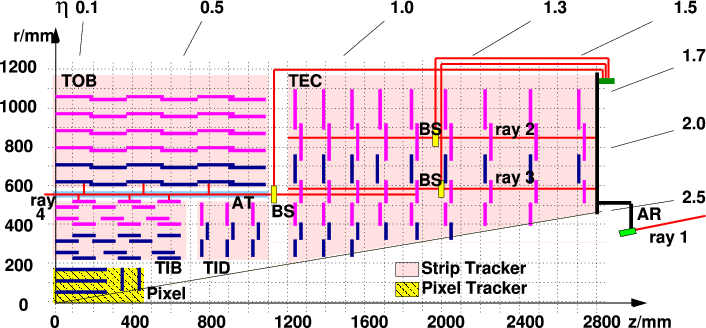
\includegraphics[width=0.98\textwidth]{Figures/c2/las}\\
\vspace{0.5cm}
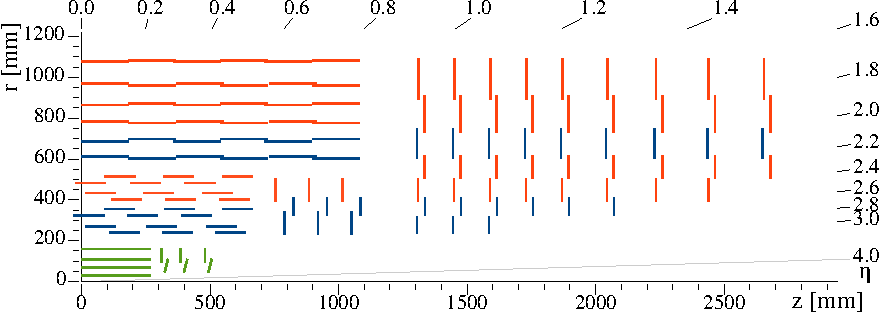
\includegraphics[width=0.68\textwidth]{Figures/c2/Phase1_Tracker_1Quarter.pdf}

\caption{Top: a quarter of the CMS silicon tracker in an $r-z$
  view. The strip tracker comprises several parts: the tracker inner
  barrel (TIB), outer barrel (TOB), inner disks (TID) and endcaps
  (TED)~\cite{Adam:1171503}. Bottom:
sketch of one quarter of the current CMS tracking system in
  r-z view, 2017-2018 data taking. The pixel detector is shown in
  green with the additional modules~\cite{trackingPU}.}
\label{fig:tracker}
\end{figure} 
Additionally the tracking system has to feature high granularity and
fast response in order to correctly associate each reconstructed track
to the respective bunch crossing and the primary interaction vertex.

The CMS tracker consists of a pixel detector (pixel Tracker) and a
silicon strip detector (strip Tracker), see Figure~\ref{fig:tracker}.
The original pixel detector was made of three barrel
layers at radii of 4.4, 7.3, and 10.2 cm and two endcaps modules in
the forward region. 
During the short shutdown between the data takings 2016 and 2017, it
was installed an
upgraded version of the pixel detector; the detector has currently four
barrel layers at radii of 3.0, 6.8, 10.2, and
16.0 cm and three layers in the forward region~\cite{Dominguez:1481838}. The
recent innermost layer and modules
are positioned closer to the beam pipe in order to improve the
precision on the position of the interaction vertices.\\
The silicon strip detector consists of many parts: the tracker inner and
outer barrels (TIB and TOB), in total ten layers of strip modules in
the barrel; the 6 tracker inner disks (TID), three each
side; and the nine disks on each side of the tracker endcap (TEC).\\
In total the tracking system is 5.8 m long and 2.6 m high,
extending the coverage of the tracker up to $|\eta|$ = 2.5. The total
amount of sensors is 66 million for the pixel and 124 million for the
strip detector. 

\subsubsection{The electromagnetic calorimeter}
The ECAL detector is a fine-grainded and homogeneous calorimeter
made up of lead
\begin{wrapfigure}{r}{0.5\textwidth}
  \begin{center}
    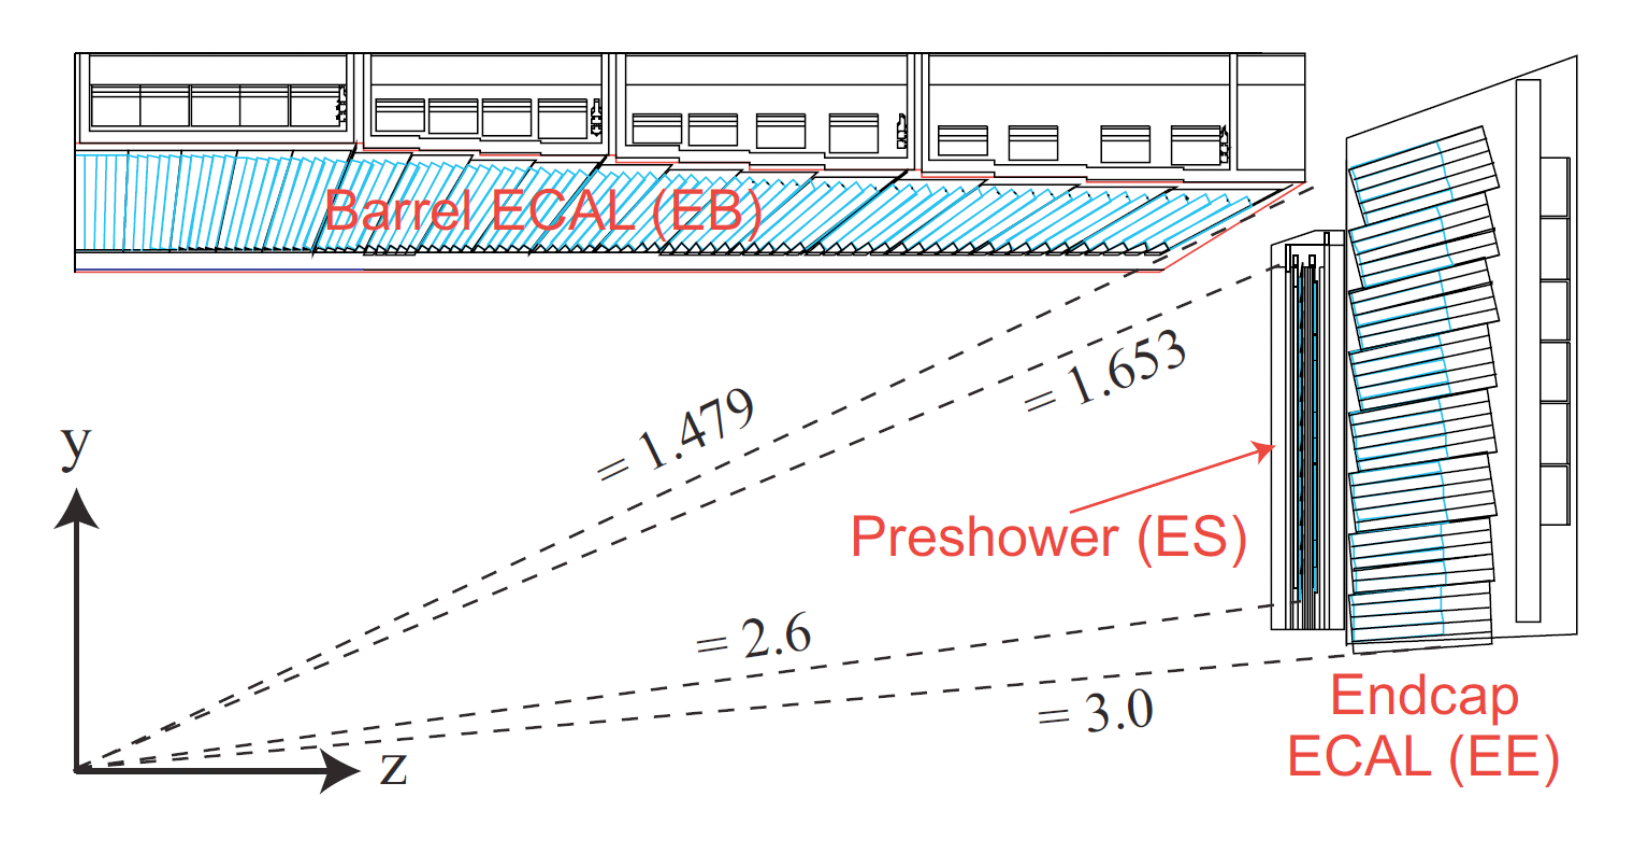
\includegraphics[clip,trim=1cm 1cm 1cm 1.5cm, width=0.48\textwidth]{Figures/c2/ecal}
  \end{center}
  \caption{Geometric view of one quarter of the ECAL~\cite{Benaglia_2014}.}
\label{fig:ecal}
\end{wrapfigure}
 tungstate crystals. Those single crystals are extremely transparent
 and ``scintillates''  when photons and electrons pass through
 them; the light produced is proportional to the particle's energy
 allowing a fast and very precise measurement of the momentum
 property. The single crystal length in barrel region is 230 mm (220
 mm in endcap) comparable to $\sim$26 (25) radiation lengths meaning it
 absorbs more than 98\% of the energy deposited by the particle~\cite{Biino_2015}.\\
A scheme of the ECAL is shown in Figure~\ref{fig:ecal}.
ECAL modules are placed in the barrel ($\eta<$ 1.479) and endcap
(1.635 $<\eta<$ 3.0) regions, and a preshower detector is located just
before the endcap crystals. The preshower detectors help CMS to
distinguish between single high-energy photons and the less
interesting pairs of low-energy photons very close to each other, \ie
coming from the decay of a $\pi^0$. 

\subsubsection{The hadron calorimeter}
The HCAL detector is a hermetic sampling calorimeter which means it
consists of alternative layers of ``absorber'' and ``scintillator''
materials that measure a particle’s position, energy and arrival time.
The quantity of light in a given position is summed up over several
layers of tiles in depth, called a “tower”, thus this total amount of
light is a measure of a particle’s energy.\\
The HCAL is located both inside the solenoid, the main part, and
outside it, the outer barrel (HO). 
Inside the magnet coil, the barrel (HB) and endcap parts (HE) cover
respectively the pseudorapidity
ranges $\eta<$ 1.3 and 1.3 $<\eta<$ 3.
The forward region of pseudorapidity is covered by the forward hadron
calorimeter (HF) up to $\eta<$ 5. It is made up of iron radiators and
quartz-fibre sensors and it measures both the electromagnetic and the hadronic shower. 
The outer barrel, HO, ensures no energy leaks out the
back of the HB undetected.

\subsubsection{The muon system}\label{sec:muonsystem}
The muon system is constructed to detect muons and to measure their trajectories.\\ 
It is composed by three different kind of gaseous particle
detectors inserted in the steel yoke. There are the drift tubes
modules, DTs, the cathode strip chambers, CSCs and the resistive plate
chambers, RPCs.\\
The four layers of DTs are located in the barrel and they cover up to
$\eta<$ 1.2 pseudorapidity range in the detector. The four layers of
CSCs are installed in the endcap covering the pseudorapidity range 0.9
$<\eta<$ 2.4. Finally there are the RPCs positioned both in barrel
and endcap parts up to $\eta<$ 1.6. The whole pseudorapidity range of
the muon system allow to measure muons up to $\eta<$ 2.4.

\begin{figure}[h]
\centering
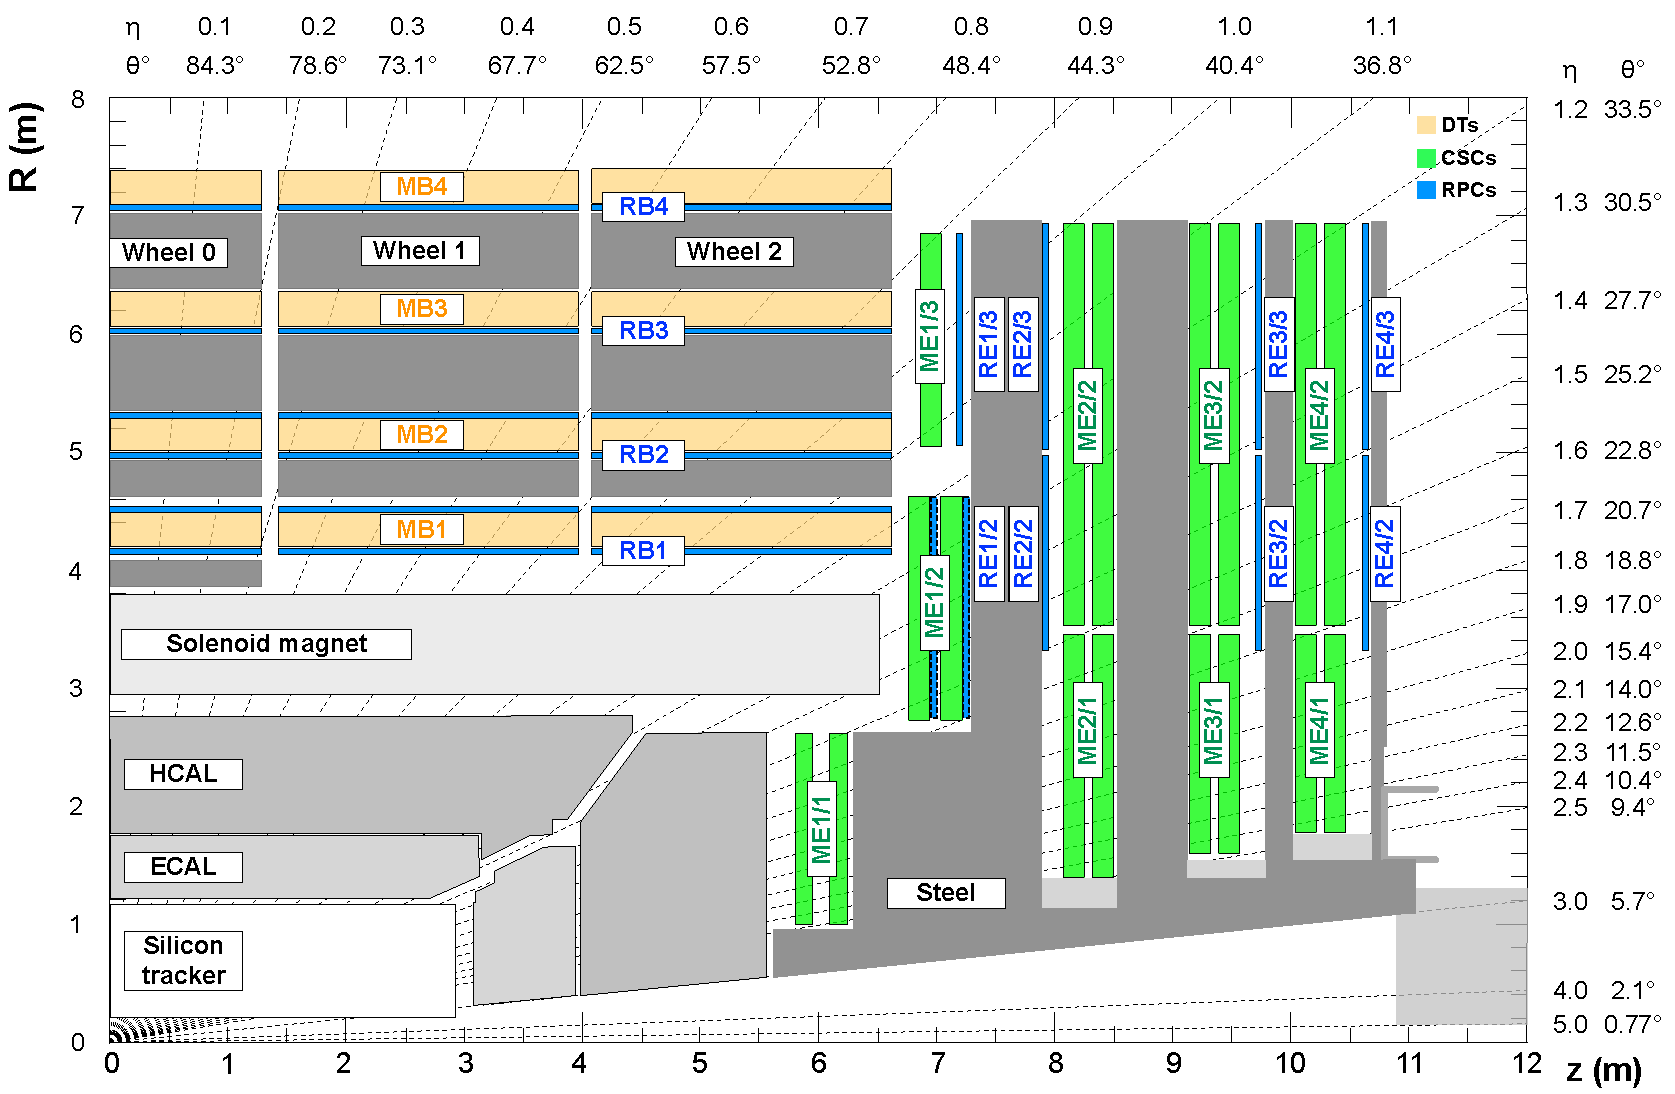
\includegraphics[width=0.98\textwidth]{Figures/c2/cms_quadrant_run_ii.pdf}
\caption{Geometric view of one quadrant of CMS. The grey areas are
  tracker, ECAL and HCAL systems, previously explained; the colored
  areas show the muon system and its subsystem. The drift tube, DTs,
  modules are labelled MB (muon barrel) and the cathode strip
  chambers, CSCs, are labelled ME (muon endcap). Resistive plate
  chambers, RPCs, are labelled RB and RE and they are mounted in both the barrel and endcaps of CMS
~\cite{muonsystemPU}. }
\label{fig:muonsystem}
\end{figure} 

\subsubsection{The CMS trigger system}\label{sec:triggersystem}

At center of the CMS detector, proton-proton collisions occur every
25 ns which means a frequency of 40 MHz. However not every collision is
necessarily of potential interest for the CMS physics program and
moreover there are technical limitations on the rate the collision data can be
saved on disk to be analyzed offline. Thus a trigger is needed to be
able to sort between potentially interesting events and the extent of
inelastic scattering events.
Since the reading and storing time of the collision data is larger
than the collision frequency the viable solution is
to store the informations in pipelines that hold and process data
from several collision at the same time.
To work without mixing particles from two different events, it is
required detectors have very good time
resolution and the signal from the millions of channels of different
systems to be synchronized and integrate.

The CMS trigger has a two-stage architecture. The first level, L1 is
implemented in custom hardware and uses informations from the 
all muon systems and the calorimeters to identify events applying a fast
basic identification of measured particles. The first step reduces the
event rate to $\sim$100 kHz.\\
The events sorted by the L1 are further refined by the
high-level trigger, HLT. It is a software farm that employs informations from all sub-detectors to perform a
refined event reconstruction reducing the rate down to a few kHz. The 
events are then saved for offline analysis.
The trigger selection is a irreversible process, what was not selected
by it is lost and it can not be recovered~\cite{Khachatryan_2017}.

A complete sequence of L1
and HLT selection criteria, including any prescale, is referred to
as a trigger path.

\clearpage
%-----------------------------------
%	SECTION 2
%-----------------------------------

\section{Event reconstruction}\label{sec:reconstruction}
With the term ``event reconstruction'' is meant the identification of
all final state particles which are produced in a proton-proton
collision. Particles are classified according to their distinct
signatures they present in 
the CMS detector, as displayed in Figure~\ref{fig:cmsslice}.

CMS detector is built with the idea of cylindrical detection layers
which are wrapped around the beam axis. After the collision, starting
from the point where the interaction occurred, particles enter in the
tracker. In the tracker charged-particle trajectories, \emph{tracks}
and origins, \emph{vertices} are reconstructed using the information from
electronic signals, \emph{hits}, in the detection layers. Subsequently
electrons and photons are absorbed in the ECAL where they stop, and
charged and neutral hadrons could start a hadronic shower in the ECAL
already and being fully absorbed in the HCAL. Muons and neutrinos cross
the full detector with little or zero interactions; the muons reaching the muon-system produce
signal hits and they trajectory is finally defined. This simple
event-view is graphically displayed in Figure~\ref{fig:cmsslice}.
\begin{figure}[h]
\centering
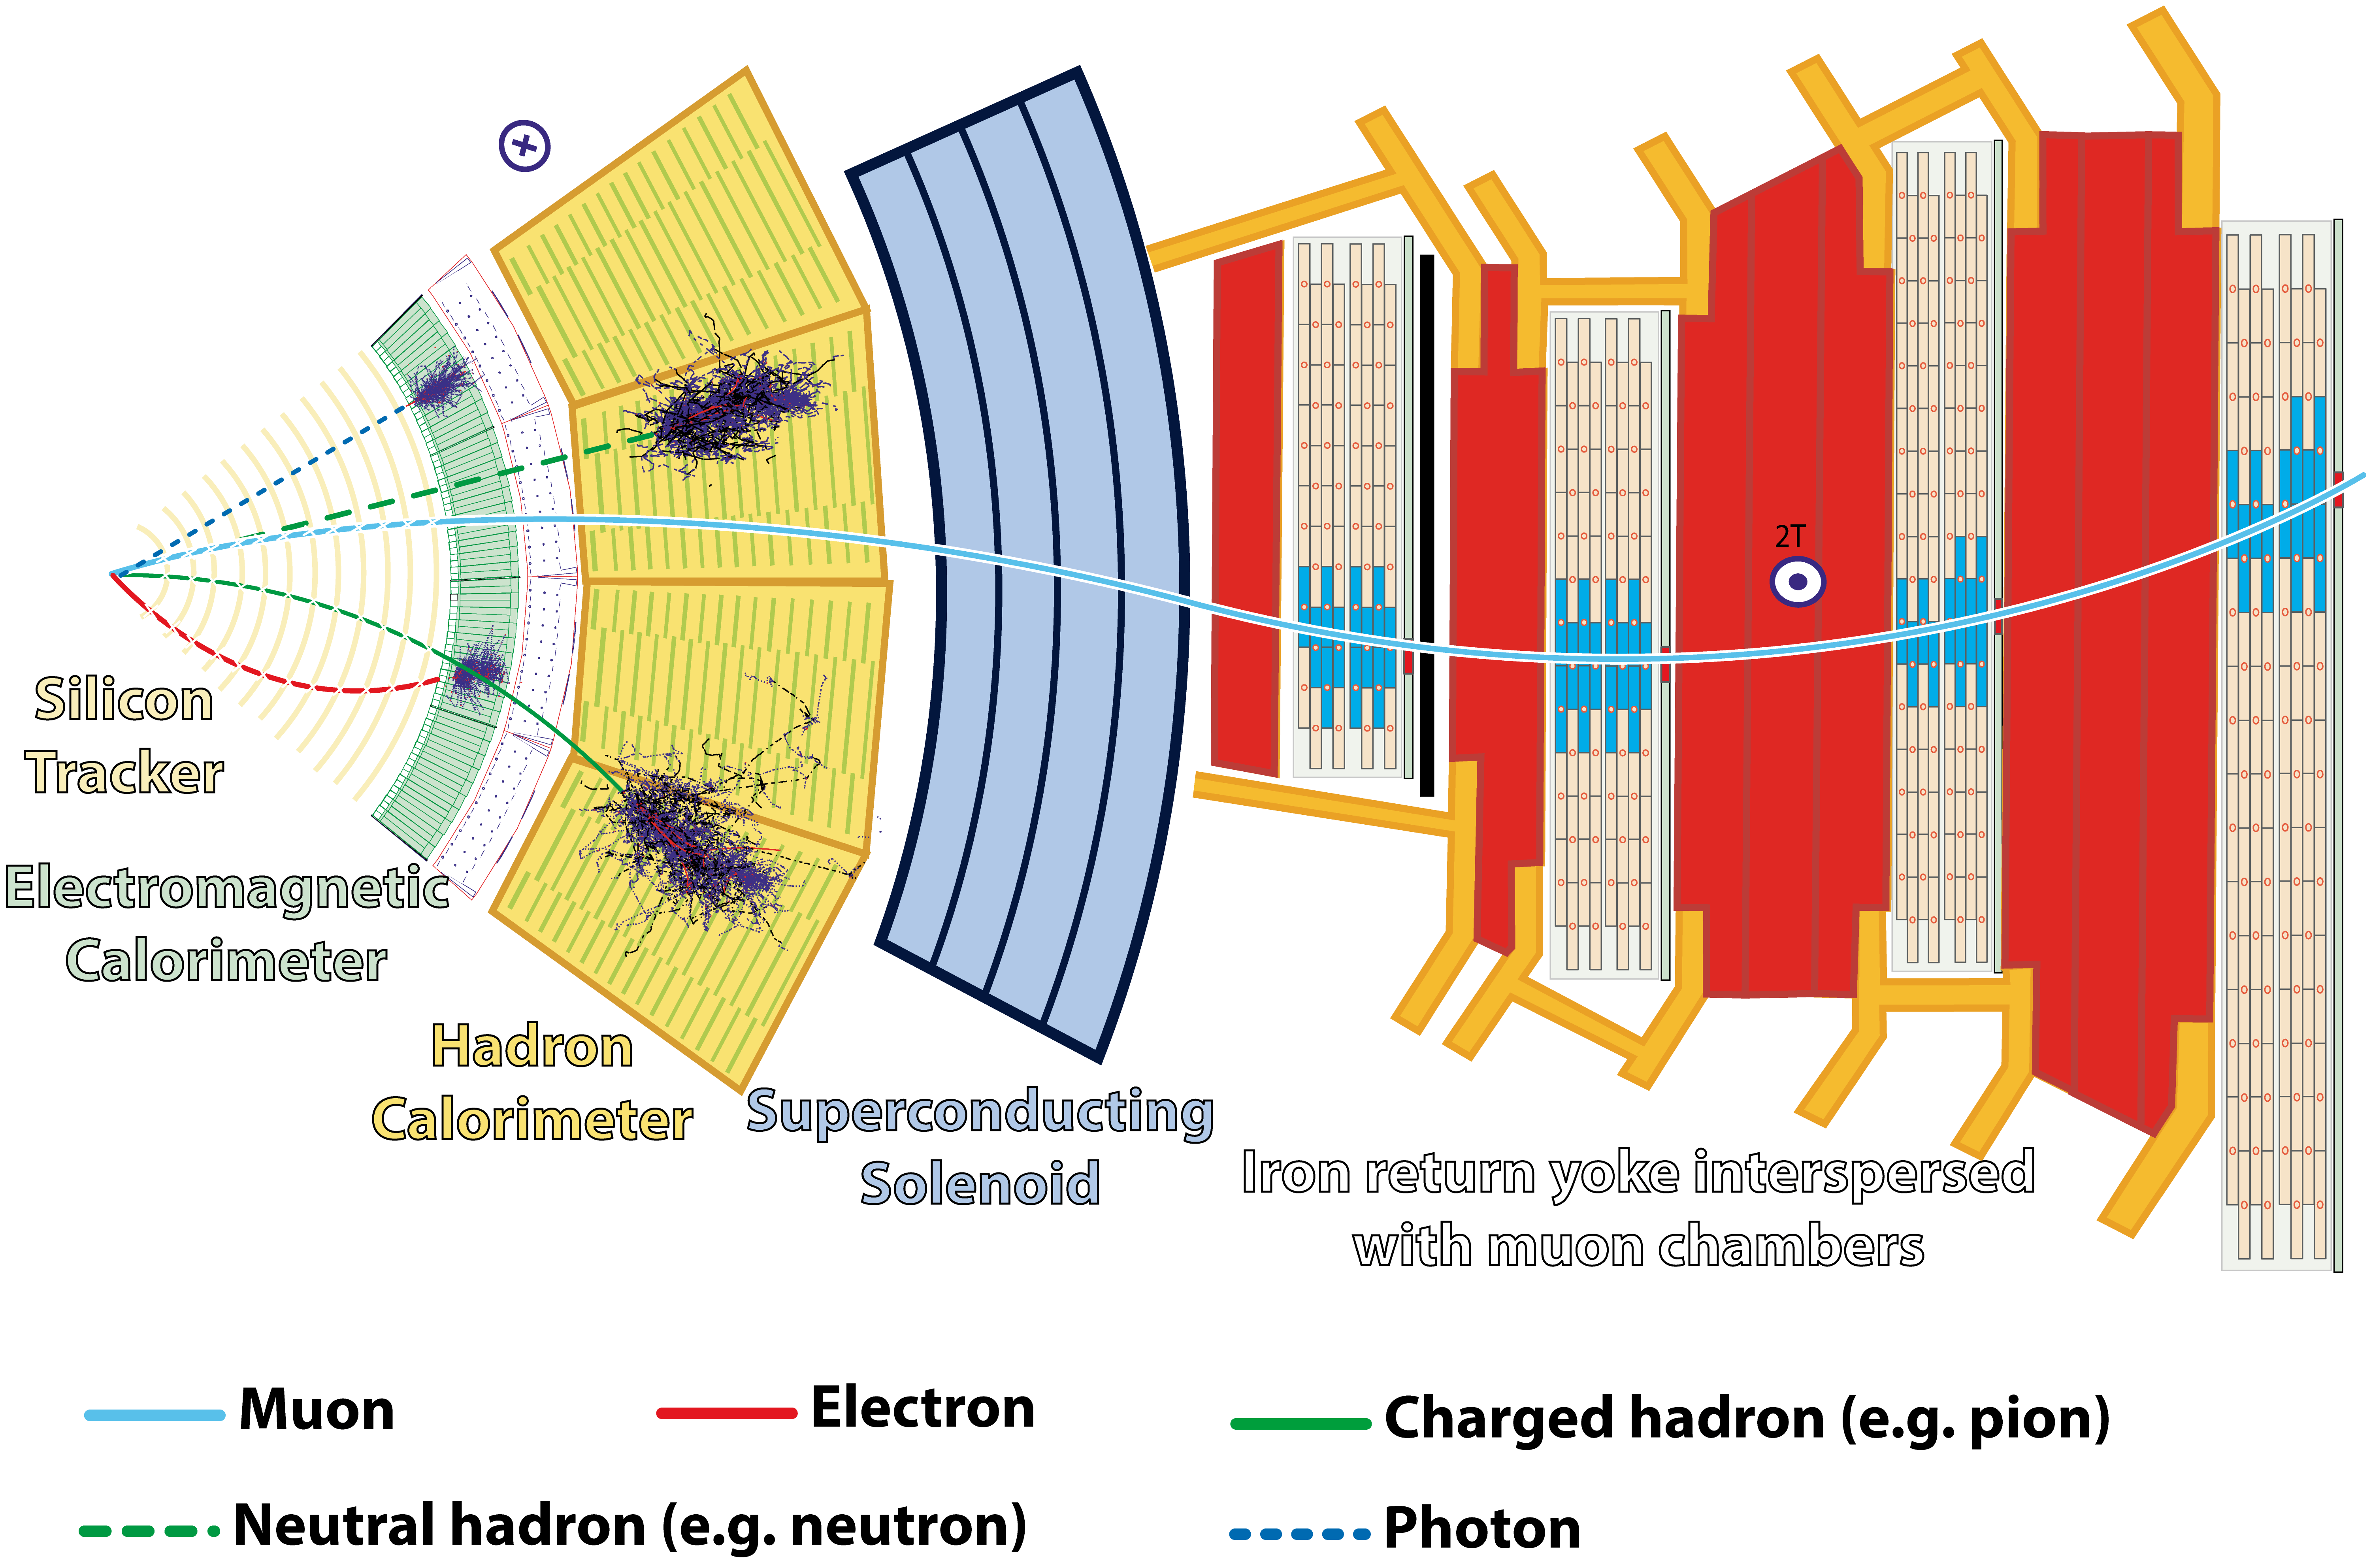
\includegraphics[width=0.78\textwidth]{Figures/c2/CMSslice.png}\\
\caption{Geometric view of a transverse slice of the CMS detector showing its sub-detectors and how particles interact with them~\cite{Barney:2120661}.}
\label{fig:cmsslice}
\end{figure} 

This approach has led to the practice of reconstructing \emph{physics
objects} in the first place using the signals collected by a specific
detector in the following way:
\begin{itemize}
\setlength\itemsep{-0.2em}
\item \emph{jets} (hadron and photons): the energy can be measured by ECAL
  and HCAL without any try to divide individual jet particles. Jet
  reconstruction can happen without the input from the tracker. The
  same idea applies to the \ptmiss;
\item \emph{isolated photons and electrons}: the reconstruction interests the
  ECAL;
\item \emph{jet tagging}: it is possible tag jets with origin from hadronic $\tau$ decay and
  from b quark hadronization. The tagging makes use of the properties of
  the related charged particle tracks, hence mostly concerns the
  tracker;
\item \emph{muons}: the identification is primarily based on the information
  from the muon-system.
\end{itemize}

An additional improvement on the event description is obtained by
correlating (\emph{linking}) the basic \emph{elements} (\ie tracks and
clusters) from all the sub-systems to classify each final-state
particle and then by combining the measurements to be able to
reconstruct the physics-object properties like mass and momentum. This
integrated approach is called \emph{particle flow} (PF)
\emph{reconstrution}~\cite{CMS:particleflow} and it is going to be
explained later in Section~\ref{sec:PF}.




This chapter details the approach and the relevant steps of the CMS
event reconstruction algorithms, paying particular attention to the
aspects pertinent to this thesis (i.e. light leptons). The track and vertex reconstruction 
is presented in Section~\ref{sec:trackvertex} and particle-flow
algorithm is described in Section~\ref{sec:PF}. Identification and
performances of muons and electrons are presented in
Sections~\ref{sec:trackmuon} and~\ref{sec:trackele}.


\subsection{Track and vertices reconstruction}\label{sec:trackvertex}

Be able to precisely reconstruct interaction vertices and charged
particle tracks is a crucial element for an accurate measurement of
charged particle momenta and properties. Tracks, vertices and their
successive combination constitute an important input for pileup
mitigation (Section~\ref{lhc}) and for the
identification displaced vertices from which particles from long-lived
particle decay originate.
Lastly tracks and vertices are fundamental inputs to the particle-flow (PF) algorithm (Section~\ref{sec:PF}).\\
The tracking algorithms are devised to
increase the track-finding efficiency while keeping small the
contamination of fake tracks, \ie tracks constructed from uncorrelated hits or
including false hits.\\
 
The tracks are reconstructed starting from the hits in the pixel and
strip tracker. The hit reconstruction follows two steps: the first,
indicated as local reconstruction, is a clustering of signals in the
tracker sensors. Thus 
the first estimate of the
position of the hit is determined based on the geometry of the single
pixel or strip while taking into consideration the Lorentz drift due
to the magnetic field (more detailed info about local reconstruction
can be found here:~\cite{CMS:particleflow}). The second step is a more
sophisticated reconstruction which uses the informations about the
irradiation status of the pixel and strip sensors. \\
The hit efficiency is measured to be above the 99.5\%\footnote{The hit
  efficiency depends on the
$d\mathcal{L}/dt$ and on the trigger rate, in particulars in
the first layer of the pixel sub-detector where the occupancy is greater.} for both pixel
and tracker hits~\cite{CMS:particleflow}. According to the size of the
cluster and the angle of
incidence of the particle, the final resolution in the
hit position is measured to be in the range of 20 (10) and 50 $\mu$m
for the pixel (strip) tracker~\cite{CMS:particleflow}.\\
An additional inputs for the track reconstruction are the identification
of the LHC beam spot position, \ie the LHC luminous region's
3D profile, and the position of the collision
vertices. 

The tracking algorithm used by CMS is called Combinatorial Track Finder (CTF)~\cite{Collaboration_2014_tracking}.
To lower the combinatorial complexity, it is applied an iterative
procedure in distinct successive iterations, each with moderate
efficiency and loosened selection requirements on the track quality with
respect to the step before. The method of Kalman
filter~\cite{BILLOIR1990219} is used for the track-finding
algorithm. While taking into account the multiple Coulomb scattering on the
direction of the track, the Kalman filter makes use of track
seeds\footnote{``\emph{The seeds define the starting trajectory parameters and associated uncertainties of potential
tracks. In the quasi-uniform magnetic field of the tracker, charged particles follow helical paths
and therefore five parameters are needed to define a trajectory. Extraction of these five parameters
requires either three 3-D hits, or two 3-D hits and a constraint on the origin of the trajectory
based on the assumption that the particle originated near the beam
spot}''~\cite{Collaboration_2014_tracking}.} 
to extrapolate the track
trajectory to the successive detector module. Thus at each layer, new
additional consistent hits
are integrated into the trajectory and the track parameters are
calculated again. The procedure starts again and the new resulting
trajectory is extrapolated to the subsequent layer. At the end, tracks
which do not fulfill goodness-of-fit requirements are rejected. Tracks
which are ``easy'' to reconstruct, e.g. from particle with large \pt
(which means less evident curvature) and produced in proximity to the
interaction point, are reconstructed first. Therefore hits associated
to these tracks are taken out making the subsequent iterations less
complex. To guarantee high efficiency, track-finding starts with
trajectory seeds which are built in the innermost region of the
tracker. 
The reconstruction efficiency for tracks with \pt $>$ 1\GeV  is measured to be larger
than 99\% for isolated muons for $|\eta| < $ 2.5 and between 80 and
99\% for electrons and pions~\cite{CMS:particleflow}. The track \pt
resolution depends on the \pt and $\eta$ of the tracks, and it is
lower than 1\% for muons with \pt $\in [1,10]$\GeV~\cite{CMS:particleflow}.

Vertices are reconstructed using the high-quality tracks which are
compatible with originating in the beam spot. They are then clustered
based on their coordinates along the \emph{z}-axis. An adaptive vertex
fitting~\cite{Waltenberger_2007} developed as an iterative re-weighted Kalman filter
is used to estimate the coordinates of the vertices. To each track it is assigned a
weight between 0 and 1 according to the probability for that track to
belong to a specific vertex. Thus vertex weights are appointed to each
vertex as the sum of the weights of all the
associated tracks, and the vertices with weights inferior predefined
thresholds are rejected. The reconstruction efficiency depends on the
number of tracks associated to the vertex and it is estimated to
be close to 100\% for the cases with more than two tracks and around
98\% for vertices with two tracks~\cite{CMS:particleflow}. The
resolutions varies between 10 and 100 $\mu$m~\cite{CMS:particleflow}.\\
The primary vertex (PV) is identified as the vertex with the largest $p^2_T$ sum for
physics-objects associated to it. The other vertices are assigned as pileup
vertices.

\subsection{The particle-flow algorithm}\label{sec:PF}

The PF algorithm~\cite{CMS:particleflow} is devised to cater a global event
description by linking and combining information from CMS
sub-detectors. 
\begin{figure}[h]
\centering
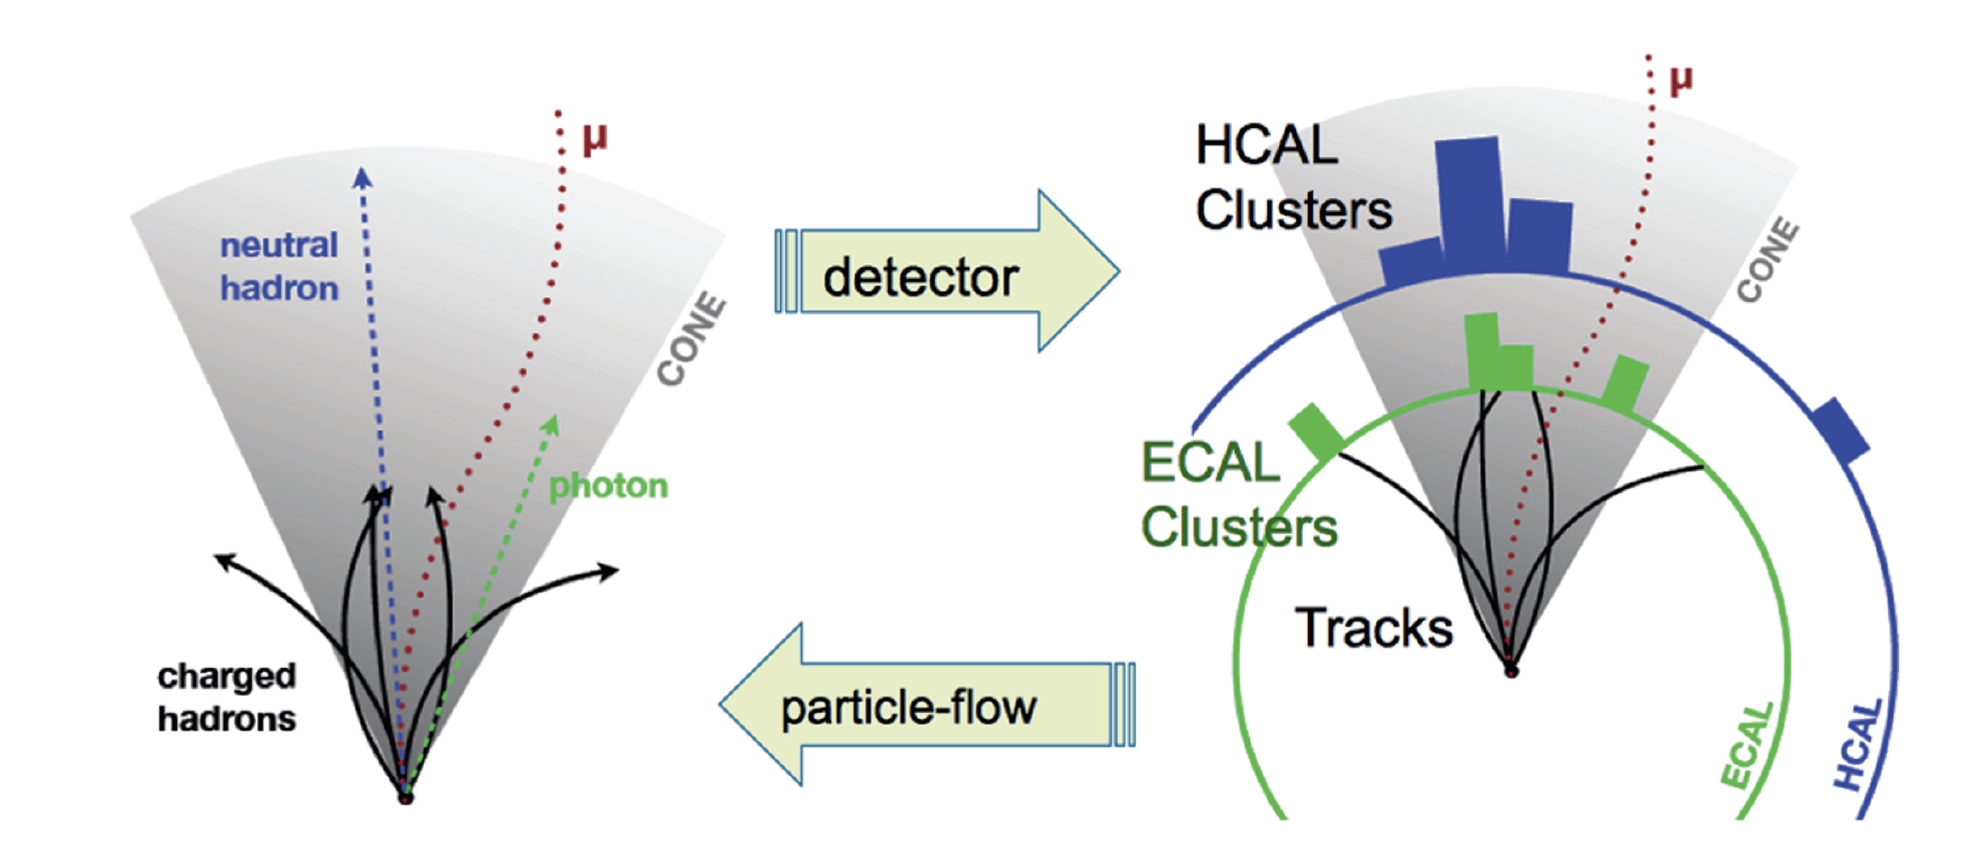
\includegraphics[width=0.58\textwidth]{Figures/c2/pfscheme}\\
\caption{The output of the PF is a list of candidates like
  electrons, muons, photons and hadrons. The PF algorithm links
  information from all the sub-system to give a global description of
  the collision event~\cite{Petrucciani:2650974}.}
\label{fig:pfscheme}
\end{figure} 

The input of the PF are the \emph{elements} tracks, vertices, tracks
reconstructed from the muon system and
calorimeter clusters. The output of the PF is a list of candidates
like electrons, muons, photons and charged and neutral hadrons (see
Figure~\ref{fig:pfscheme}). The identification of leptons, the
measurement of the \ptmiss and the categorization of the pileup tracks
are improved by the usage of the PF algorithm. When linking
information from tracker and calorimeters signals, noticeable gain is seen
in the angular momentum resolution of jets~\cite{CMS:particleflow}.

\subsubsection{Jet clustering and reconstruction}\label{sec:jetclustering}
Jets reconstruction is performed with a recombination algorithm which
is known as anti-$k_T$ algorithm (with distance parameter of cone size
of $\Delta R = 0.4$). The detailed description of the anti-$k_T$ algorithm is not
discussed in this work but all the information can be found in 
references~\cite{Cacciari_2008,Cacciari_2012}.

In order to reduce the number of jets rising from mis-reconstruction or
detector noise, identification requirements are applied depending on the single elements of the
jets meaning the number of particles and the amount of energy of the
jet which comes from different type of PF candidates~\cite{CMS-PAS-JME-16-003}.
The jet energy is set as the vectorial sum of the momenta of the
particles constituting the jet. In order to alleviate the effect of
pileup contribution in the jet reconstruction, charge hadrons
associated to pileup vertices do not enter in the jet clustering. This
scheme is known as ``charge hadron
subtraction''~\cite{CMS-PAS-JME-14-001} and removes a
considerable fraction of charged pileup particles.  
Subsequently it is applied a correction to account for the
contribution from neutral particles from pileup; the subtraction is
based on the average transverse momentum, \pt, per unit area in the
pileup jets~\cite{CACCIARI2008119, Cacciari_2008_area,
  Sirunyan:2020foa}.

Corrections on the jet energy are applied in order to correct for the
remaining pileup energy contributions and for any discrepancies
between jet properties in measured data and in simulated events. Those
correction are obtained from the ratio between the \pt of a
reconstructed jet and its corresponding generated jet and they are
measured as function of \pt and $\eta$ and applied to data and
simulation~\cite{Khachatryan_2017}. The jet \pt resolution is
derived both in data and MC and the resolution in the simulation is
fixed and smeared to match the one in the
data~\cite{Khachatryan_2017}.

\subsubsection{Tagging of jets originating from b
  quarks}\label{sec:tagging}
The identification of jets which originate from b quarks, called
b jets, can be achieved using
specific properties and features of heavy
quarks inside the jet. This technique, usually called b tagging, is
extremely important to discriminate between signal and background as
it will be analyzed and explained in Chapters~\ref{Chapter5}
and~\ref{Chapter6}.
\begin{figure}{h}
  \begin{center}
    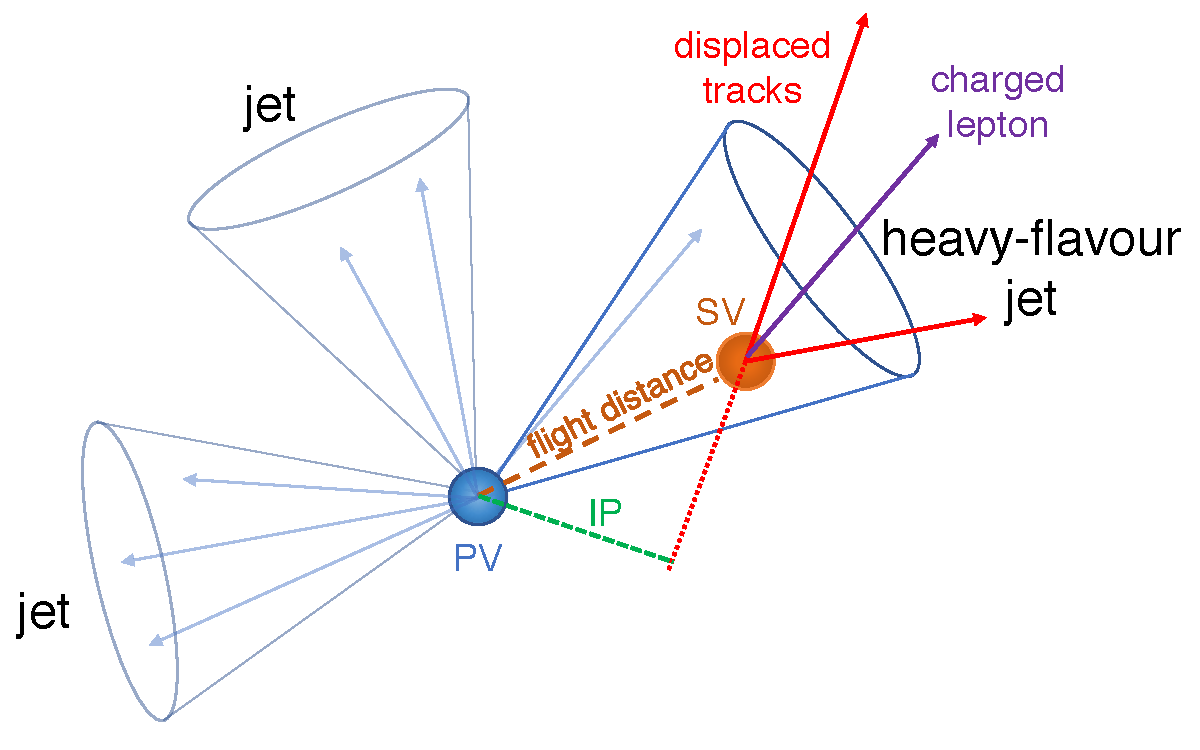
\includegraphics[clip,trim=0.3cm 0.5cm 0.3cm 0.3cm, width=0.50\textwidth]{Figures/c2/tagging}
  \end{center}
  \caption{Schematic view of a b jet with a SV from the decay of a b hadron resulting in tracks which are displaced with respect to the PV, and hence with a large impact parameter (IP) value~\cite{Sirunyan_2018_tagging}.}
\label{fig:btagging}
\end{figure}

The b jets contain b hadron that have a lifetime of the order of 1.5
ps and a mass of about
5\GeV. Thus the b hadrons can propagate from
the PV for a few mm up to a few cm before decaying. This results in
a secondary vertices (SVs) which contain displaced tracks, see
Figure~\ref{fig:btagging}. With respect to light jets (coming from
u, d, s quarks or gluons) b jets have larger mass and harder hadronization which
means that the decay products have larger momentum and larger number
of tracks related with the jet. These signatures are exploited by the
algorithms allowing to construct variables to separate b jets from
light jets. The results of the b tagging are discriminator values for
jets, see Figure~\ref{fig:taggingperformance}; large discriminator values coincide with higher probability for
the jet to be a jet originating from b hadrons~\cite{CMS-DP-2017-013,
  csv}.\\
The b tagging performances are checked in terms of the b jet
efficiency (which expresses the fraction of all b jets truly coming from b hadron
that are identified as b jets) and of misidentification probability
(which expresses the fraction of light jets or jets from c hadrons
which are identified as b jets), see
Figure~\ref{fig:taggingperformance}. 

\begin{figure}[h]
\centering
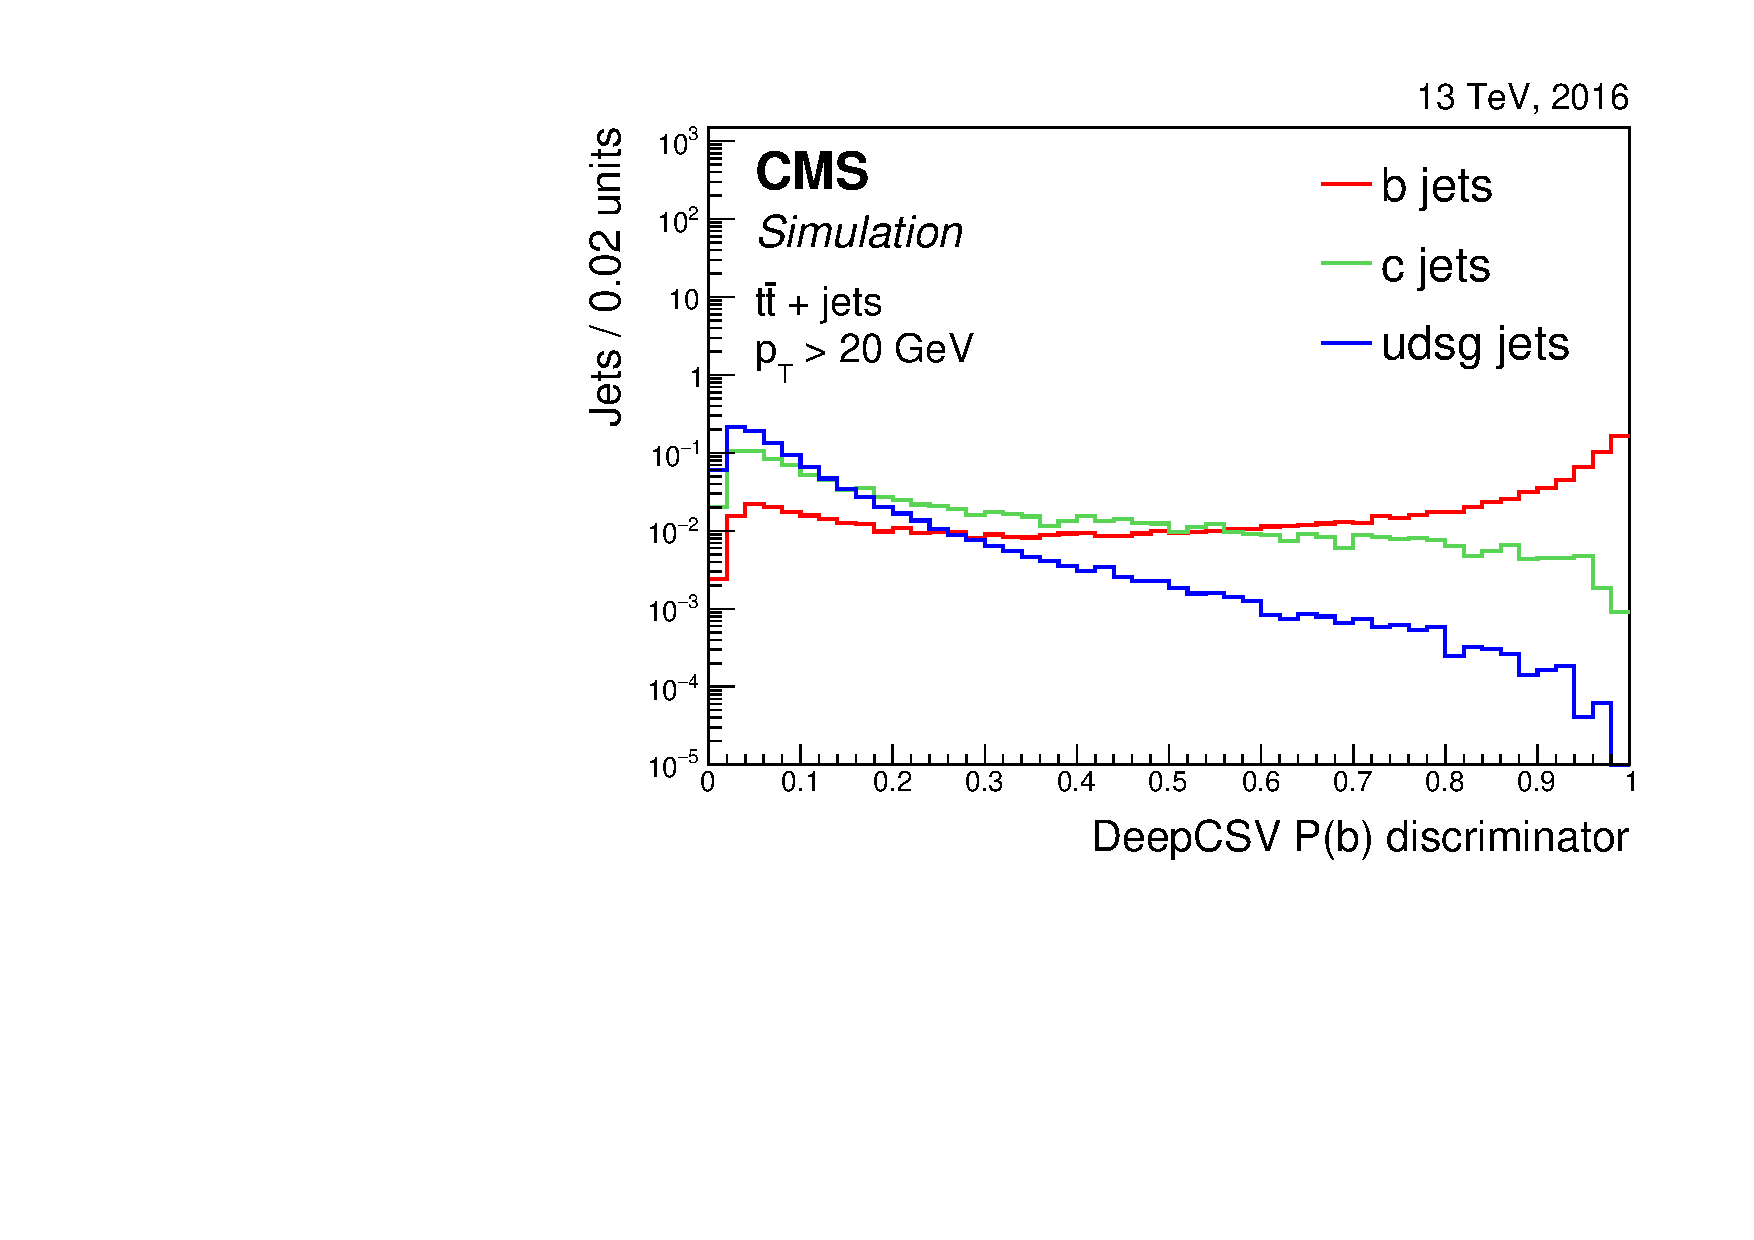
\includegraphics[width=.49\textwidth]{Figures/c2/CMS-BTV-16-002_Figure_013-a.pdf}
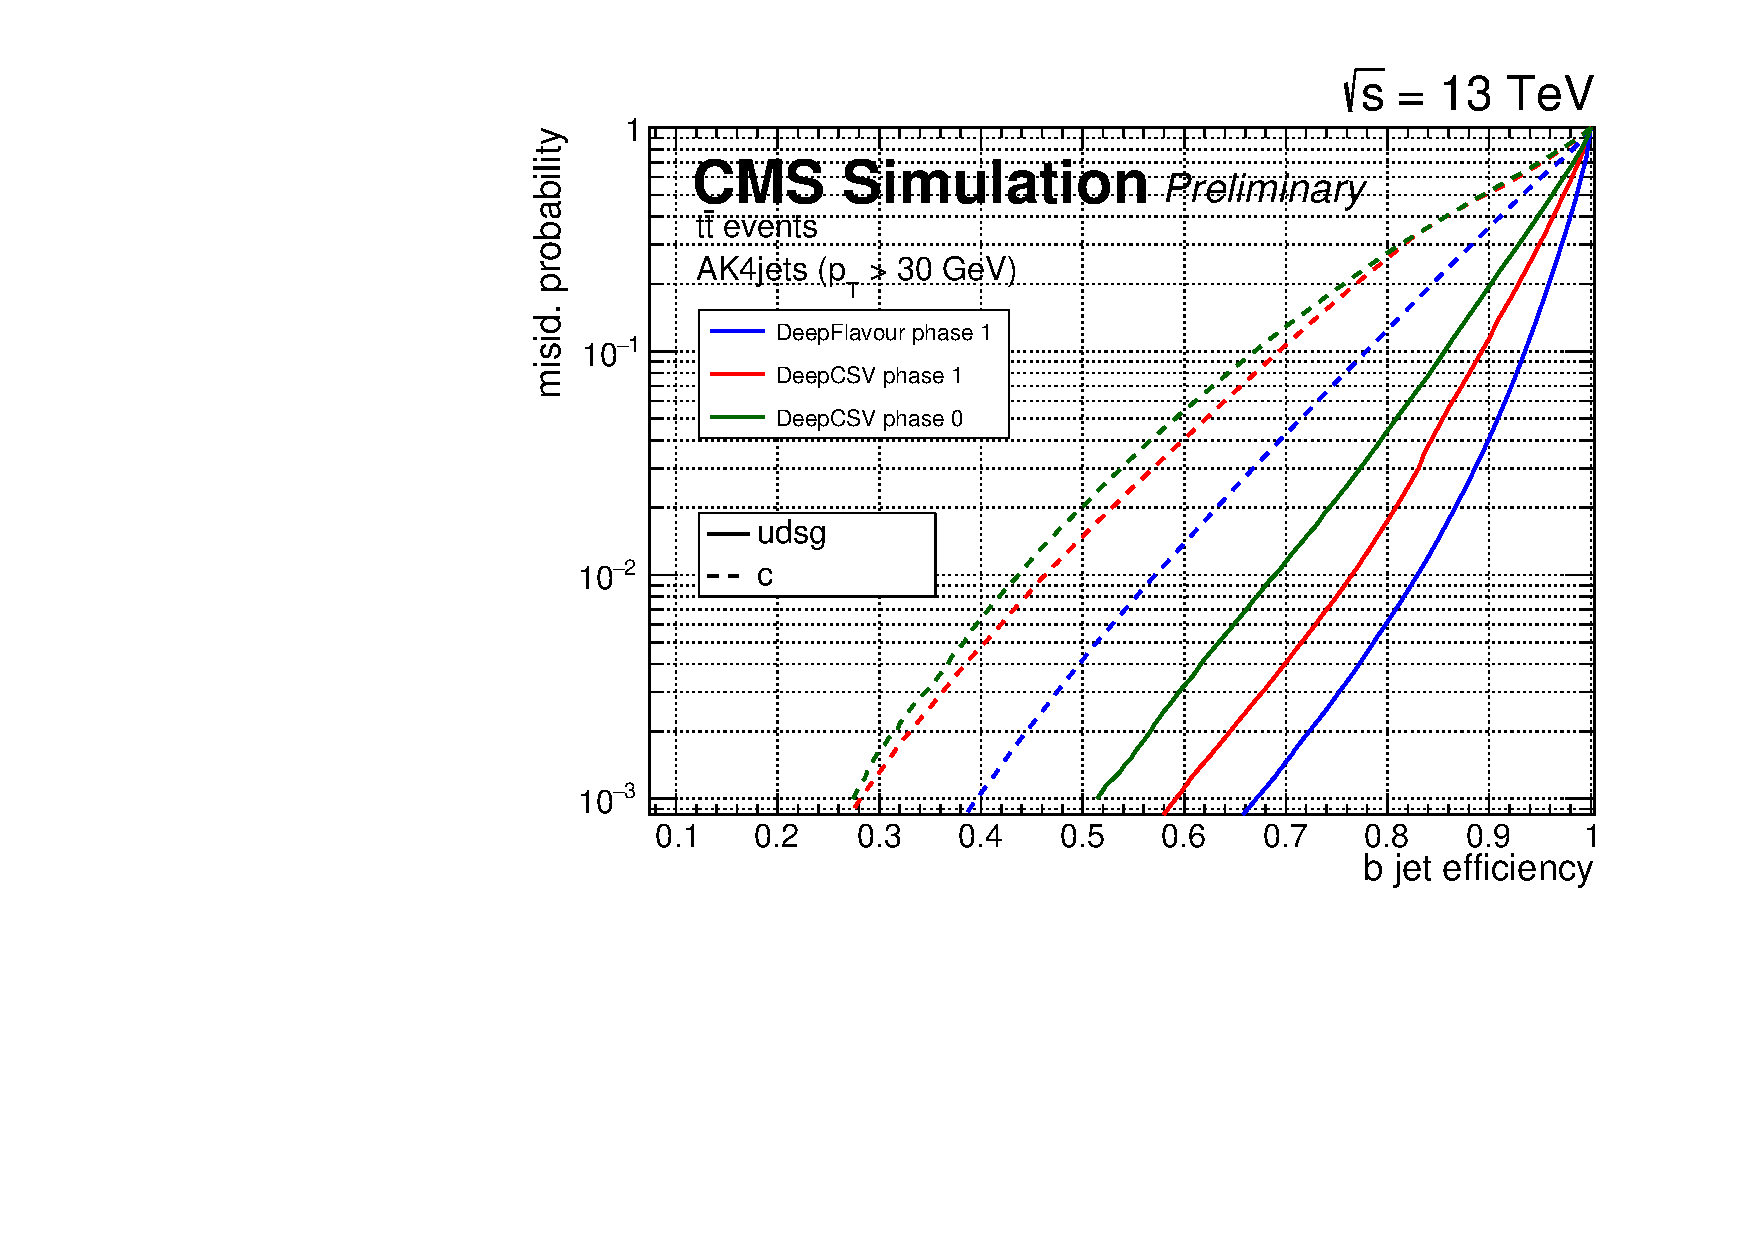
\includegraphics[width=.49\textwidth]{Figures/c2/PT30GeV.pdf}
\caption{On the left, ``performance of the DeepCSV and DeepFlavour b
  jet identification algorithms demonstrating the probability for
  non-b jets to be misidentified as b jet, as a function of the
  efficiency to correctly identify b jets. For comparison, the performance of DeepCSV
  with the 2016 detector (Phase 0) are also shown.''~\cite{csv}. On
  the right, ``Distribution of the DeepCSV P(b) discriminator values
  for jets of different flavors in \ttbar events. Jets without a
  selected track and without a secondary vertex are assigned a
  discriminator value of 0. The distributions are normalized to unit area''~\cite{csv}.}
\label{fig:taggingperformance}
\end{figure}

Here the two algorithms are known as DeepCSV~\cite{csv} and 
DeepJet~\cite{deep}. The first is the \emph{deep combined secondary vertex}, DeepCSV,
algorithm based on a fully-connected neural networks with a fixed set
of input variables for preselected tracks and preselected SVs and
kinematic features of the jets. The DeepJet~\cite{deep} is a improved
version of the DeepCSV. It is based on a deep neural network
architecture and it does not require any prior preselections and uses
a bigger number of SVs, tracks and neutral hadrons.
Looking at the right plot of Figure~\ref{fig:taggingperformance},
fixing the misidentification probability the DeepCSV has lower b jet
efficiency than DeepJet algorithm.\\
The efficiencies are calculated both in data and MC and the
corrections for the discrepancies observed between data and MC are
applied to simulated events as per-jet scale factors~\cite{csv}.


\subsection{Muon reconstruction}\label{sec:trackmuon}
This paragraph primarily describes the prompt muon reconstruction (~\ref{sec:c2muonselection}) and
identification (~\ref{sec:c2muonreco}). It will follow a short description of the displaced
case and the improved algorithms which have been designed for these specific
scenarios (~\ref{sec:c2muondisplaced},~\cite{CMS-DP-2015-015}).

\subsubsection{Muon track reconstruction}\label{sec:c2muonreco}
Muon tracking~\cite{collaboration_2013,Sirunyan_2018_muon} makes use of information from
both inner tracker and muon systems. The
inner tracker gives a precise measurement of the muon momentum; the
muon system identifies muon objects over a wide acceptance with high efficiency. A high purity in muons is obtained
thanks to the upstream ECAL and HCAL which absorb other particles
(except neutrinos). \\
According to the tracking algorithms which are used, three kinds of muon
candidates are defined~\cite{Sirunyan_2018_muon}:
\begin{itemize}
\setlength\itemsep{-0.2em}
\item \textbf{standalone muon}. The tracks are built from the
  information from all the muon sub-detectors, CSC, DT and RPC. It
  starts from seeds consisting of groups of DT or CSC segments, and
  the seeds are used for the pattern recognition in the muon system, to
gather all DT, CSC, and RPC hits along a muon trajectory using a
Kalman filter technique. The outcome of the fitting is called a
\emph{standalone-muon track}.
\item \textbf{tracker muon}. These tracks are formed
  ``inside-out''. They are extrapolated from the inner
  tracker to the muon system with loose matching to DT and CSC
  segments -- each inner track that has \pt$>0.5$\GeV and total
  momentum $>2.5$\GeV is extrapolated to the muon chambers and if at
  least one muon system segment matches that track than the muon track is defined as \emph{tracker
  muon track} --. 
\item \textbf{global muon}. These tracks are built
  ``outside-in''. They the results of the matching between
  standalone-muon tracks and tracker tracks. The matching is performed by
  comparing tracks parameters which are propagated onto a shared
  surface. Using data from both the two tracks, it is performed the final combined fit with the Kalman filter technique.
\end{itemize}

About 99\% of the muons produced within $\eta < 2.4$ are reconstructed
either as a global muon track or as a tracker muon track (or
both). In case a global muon and a tracker muon share the same inner
track, they are then merged in one single candidate.
Global muons reconstruction is meant to be very efficient for muons
which penetrate
through more than one layer of the muon system. This implicitly
requires the muon track to be more than 10\GeV since softer muons
easily fail this due to larger multiple scattering in the material of the return yoke; for the cases with
\pt$< 10$\GeV, the tracker reconstruction becomes then more efficient.
For muons which are not global muons and
they are matched with the innermost muon station only,
the probability for misidentification increases. The possibility for
hadron shower to reach the innermost muon station (punch-through)
becomes not negligible. In order to mitigate this effect additional
quality criteria on the muons are required at a later stage (described
in the following paragraph~\ref{sec:c2muonselection}).
By using the information from both the
inner tracker and the muon
system, the \pt resolution and measurement of global muons is improved
in particular for \pt $> 200$\GeV. For the case of standalone-muon
tracks, the muons have worse momentum resolution and a higher
contamination of cosmic muons than global or tracker muons.

Reconstructed muon tracks are given as input to the PF algorithm which
combines then all the information gathered from the different
sub-detectors. For muon case PF applies a list of selection criteria
to the candidates which have been reconstructed with standalone, track
and global muon algorithms. 

\subsubsection{Muon identification}\label{sec:c2muonselection}
According to the desired compromise, for each CMS search, between efficiency and purity, a
set of different variables and selections is defined~\cite{Sirunyan_2018_muon}.\\
This level of details, here described, is going to be recalled and
used in Chapter~\ref{Chapter6} where a customized and mindful selection is needed
for the displaced muon case (specifically Section~\ref{sec:c6muons}).

Some variables are related to the muon reconstruction itself. We can
list the \emph{track fit $\chi^2$}, the number of hits per track (it refers
to inner tracker hits, \emph{fraction of valid tracker hits}) and for global muons, the
level of \emph{position matching} between the tracker tracks and the standalone muon
tracks. Additionally the \emph{muon segment
compatibility} is an important parameter which returns values between 0
and 1 with 1 being the highest degree of compatibility. A \emph{kick
  finder} algorithm is deployed to evaluate a posteriori for each muon
track the
probability of being a single track or the combination of two
separated tracks.  \\
Other variables benefit from inputs from outside the muon track
reconstruction itself such as the track-PV compatibility.

Exploiting these variables, three main identification types of muons
are used in CMS physics analyses:
\begin{itemize}
\setlength\itemsep{-0.2em}
\item \emph{Loose muons identification, (Loose ID)}. A loose muon is either a
  tracker muon or a global muon. Loose ID tries to identify muons
  coming from the PV and from light and heavy flavor decay keeping
  very high selection efficiency and rather low misidentification rate
  of charged hadrons as muons. 
\item \emph{Medium muons identification, (Medium
    ID)}~\cite{PetruccianiBotta}. This selection aims to achieve, with
  respect to Loose ID, more rejection	
of muons from hadron decays in-flight while preserving
high selection efficiency. Medium muons are loose muons with tracker
tracks which have at least 80\% of valid hits in the inner tracker. 
If the muon is only a tracker muon (not a global muon), the muon
segment compatibility has to be larger than
0.451. If the muon is both a tracker muon and a global muon, ``the
muon segment compatibility need only be greater than 0.303, but then the global fit
is required to have goodness-of-fit per degree of freedom ($\chi^2$/dof) less than 3, the
position match between the tracker muon and standalone-muon must have $\chi^2$ < 12,
and the maximum c2 computed by the kink-finding algorithm must be less than 20.
The constraints on the segment compatibility were tuned after application of the
other constraints to target an overall efficiency of 99.5\% for muons from simulated
\PW and \PZ events.''~\cite{Sirunyan_2018_muon}.
\item \emph{Tight muons identification, (Tight ID)}. A tight muon must
  be reconstructed both as global muon and tracker muon. With respect
  to the Medium ID, the Tight ID requirements are more stringent on
  the number of muon stations which have to match with the inner
  tracker track and on the compatibility between track and PV. 
\end{itemize}
There are other two identification types of muons, \emph{soft muon ID}
and \emph{high momentum muon ID} which are not used in the context of
this thesis analysis and therefore are not detailed in this section. 

\paragraph{Muon isolation}\label{sec:muoniso}
To discriminate between prompt muons and muons coming from either the decays
of heavy-flavor hadrons or the decay in flight of charged $\pi^{\pm}$s and kaons, the isolation variable appears to be one of
the most critical variable to use. The PF isolation of a reconstructed
leptons is defined relative to its \pt as the scalar
sum of the energy of all the PF candidates emitted around the
direction of the muon in the cones, $\Delta R = \sqrt{(\Delta
  \phi)^2+(\Delta \eta)^2}$, surrounding the object.\\
For the estimation of the PF isolation~\cite{CMS:particleflow}, it is computed the sum of the
\pt of charge hadrons and the \pt of neutral particles (hadrons
and photons) originating from the PV. Typical values used for  $\Delta
R$ are 0.3 and 0.4.\\
A correction is applied to account for the contribution from pileup to the
neutral particles component~\cite{Sirunyan_2018_muon}.

\paragraph{Tracking and reconstruction efficiencies.}\label{sec:c2effmuon}
The efficiencies of the muon reconstruction and identification are
estimated in data and simulation events with a \emph{tag-and-probe}
method. The events are selected with two muons whose invariant mass,
$M_{\mu \mu}$, is compatible with the \PZ mass. One of the two muons,
the \emph{tag}, is selected with tight requirements. The value of the
efficiency for a specific selection (reconstruction or identification
variables) is given by the fraction of the other muons, the
\emph{probes}, which pass that specific selection. The differences in
efficiencies between data and simulation samples are accounted and
then corrected with per-muon scale factors applied to the simulated
events~\cite{Sirunyan_2018_muon}. The performances of muon
reconstruction and identification in CMS using the data collected in
2016 are shown in Figure~\ref{fig:2016eff} (details and 2017-2018
results in the reference here:~\cite{CMS-DP-2017-007,CMS-DP-2018-042})

\begin{figure}[h]
\centering
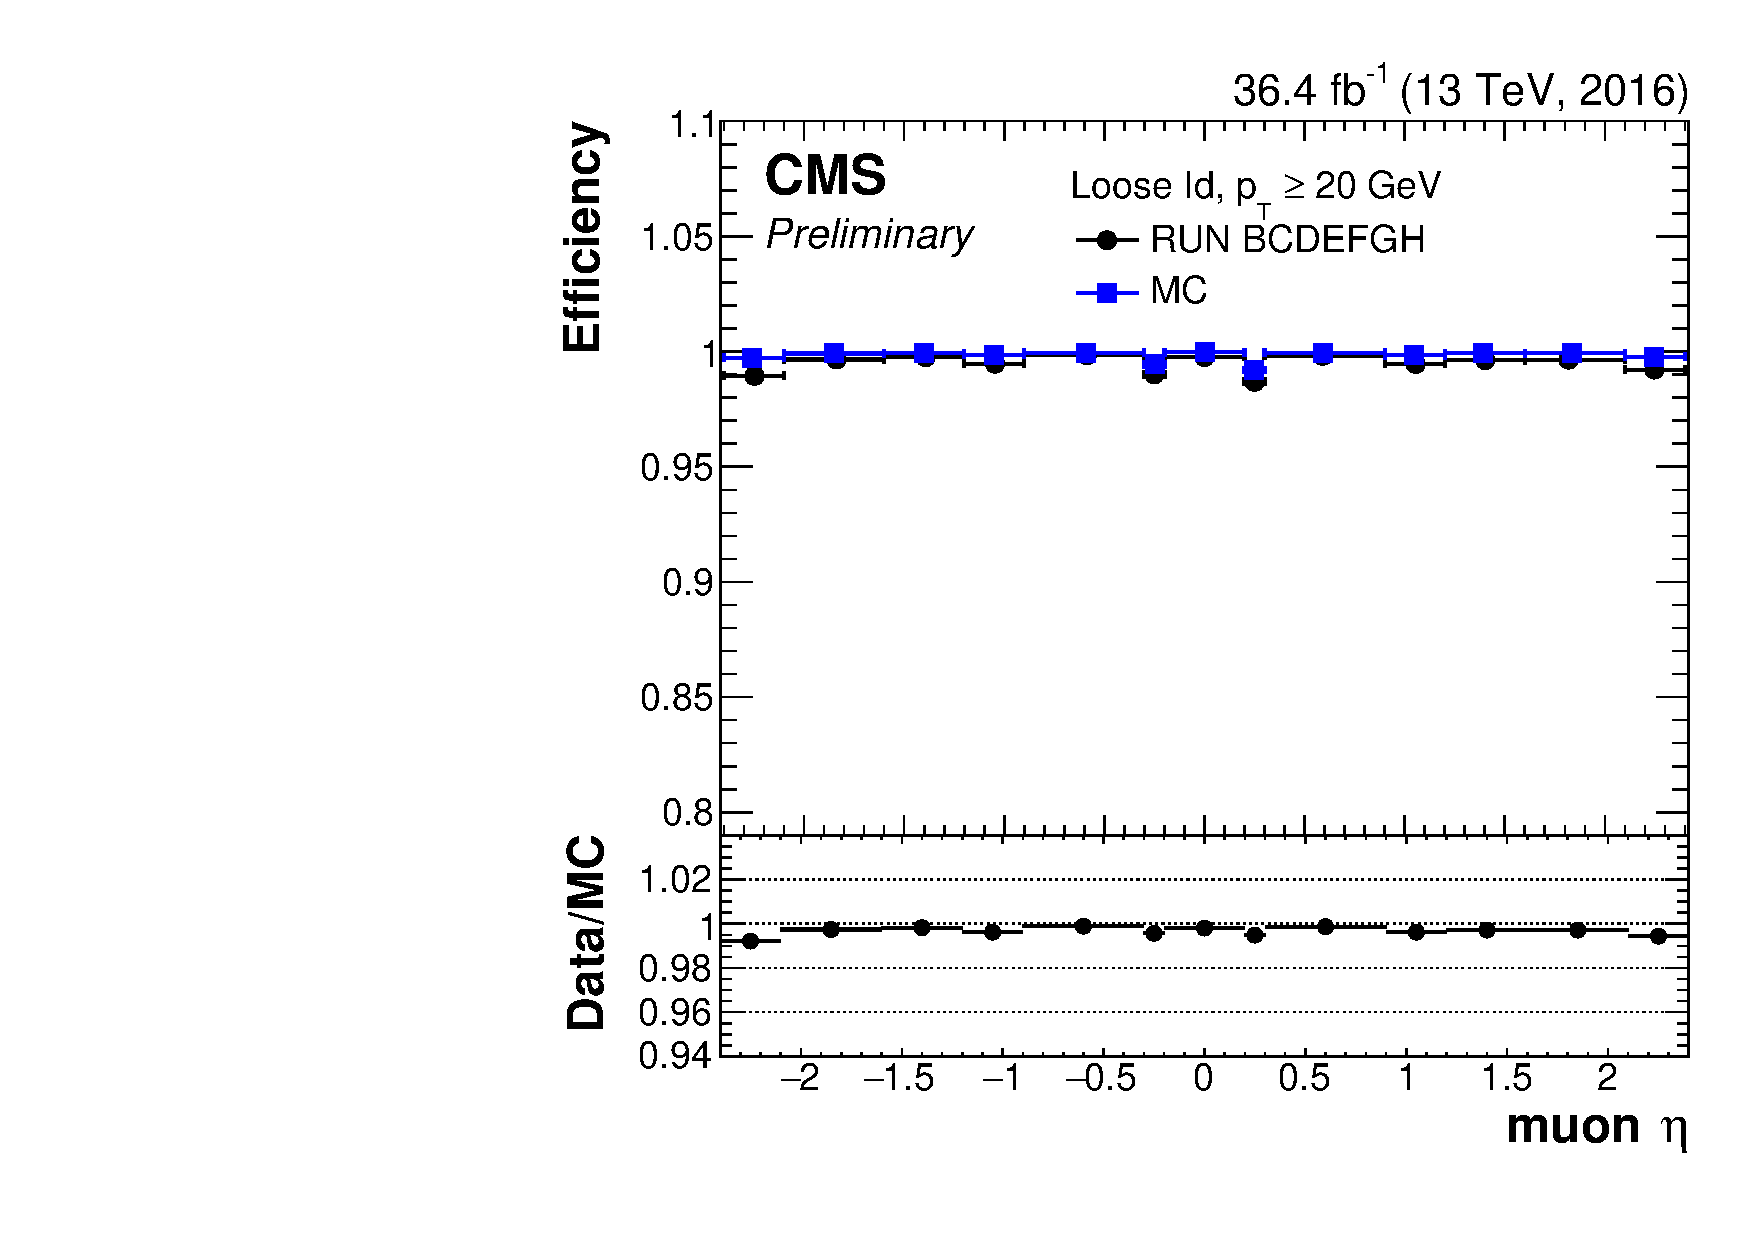
\includegraphics[width=.49\textwidth]{Figures/c2/TnP_MC_NUM_LooseID_DEN_genTracks_PAR_eta_.pdf}
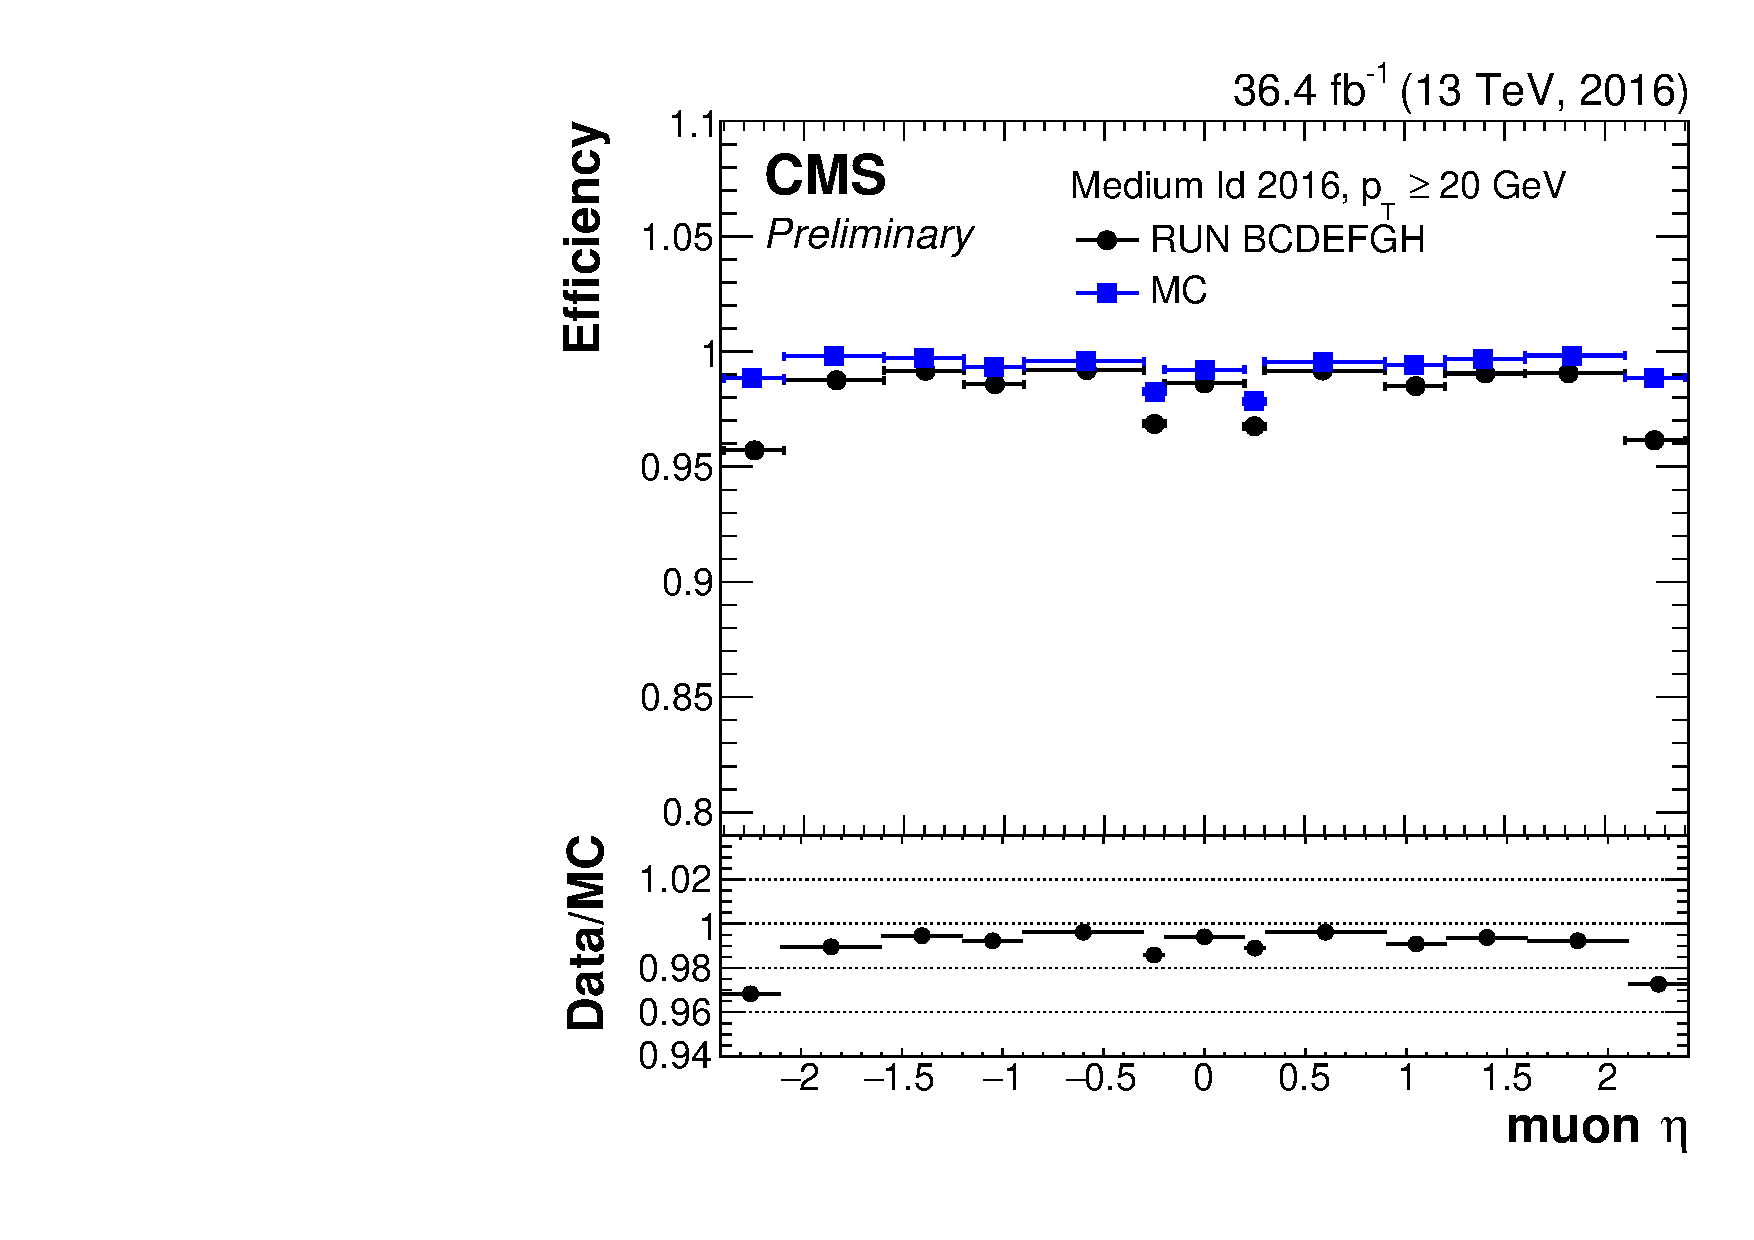
\includegraphics[width=.49\textwidth]{Figures/c2/TnP_MC_NUM_MediumID2016_DEN_genTracks_PAR_eta_.pdf}
\caption{Tag-and-probe efficiency for muon identification in 2016 data
  (circle) and simulation (squared). On the left, Loose ID efficiencies as function of $\eta$. 
On the right, Medium ID efficiencies as function of $\eta$. The
  denominator contains tracker muons. Error bars in the plots include only statistical uncertainty~\cite{CMS-DP-2017-007}}
\label{fig:2016eff}
\end{figure}


\subsubsection{Displaced muon reconstruction.}\label{sec:c2muondisplaced}
~\cite{CMS-DP-2015-015}

\subsection{Tracking for electrons}\label{sec:trackele}



\paragraph{Muon and electron Isolation}\label{sec:muoniso}
To discriminate between prompt leptons and leptons coming from either the decays
of heavy-flavor hadrons or the decay in flight of charged $\pi^{\pm}$s and kaons, the isolation variable appears to be one of
the most critical variable to use. The PF isolation of a reconstructed
leptons is defined relative to its \pt as the scalar
sum of the energy of all the PF candidates emitted around the
direction of the lepton in the cones, $\Delta R = \sqrt{(\Delta
  \phi)^2+(\Delta \eta)^2}$, surrounding the object.\\
For the estimation of the PF isolation~\cite{CMS:particleflow}, it is computed the sum of the
\pt of charge hadrons and the \pt of neutral particles (hadrons
and photons) originating from the PV. Typical values used for  $\Delta
R$ are 0.3 and 0.4.\\
A correction is applied to account for the contribution from pileup to the
neutral particles component~\cite{Sirunyan_2018_muon}.



~\cite{CMS:particleflow}
~\cite{Collaboration_2014_tracking}
~\cite{Collaboration_2010_alligment}


Figure 16 shows the invariant mass distribution of oppositely charged muon pairs selected by
the inclusive trigger on isolated double-muons. The x-axis is logarithmic so the entries are
scaled to the width of each bin. Data are also included from specific double-muon triggers
tuned to select resonances at low invariant mass. The figure clearly demonstrates the ability of
CMS to identify muons, trigger on them, and reconstruct the muon kinematics to unambiguously
identify particles that decay into muons over a broad energy range.
 \begin{figure}[h]
\centering
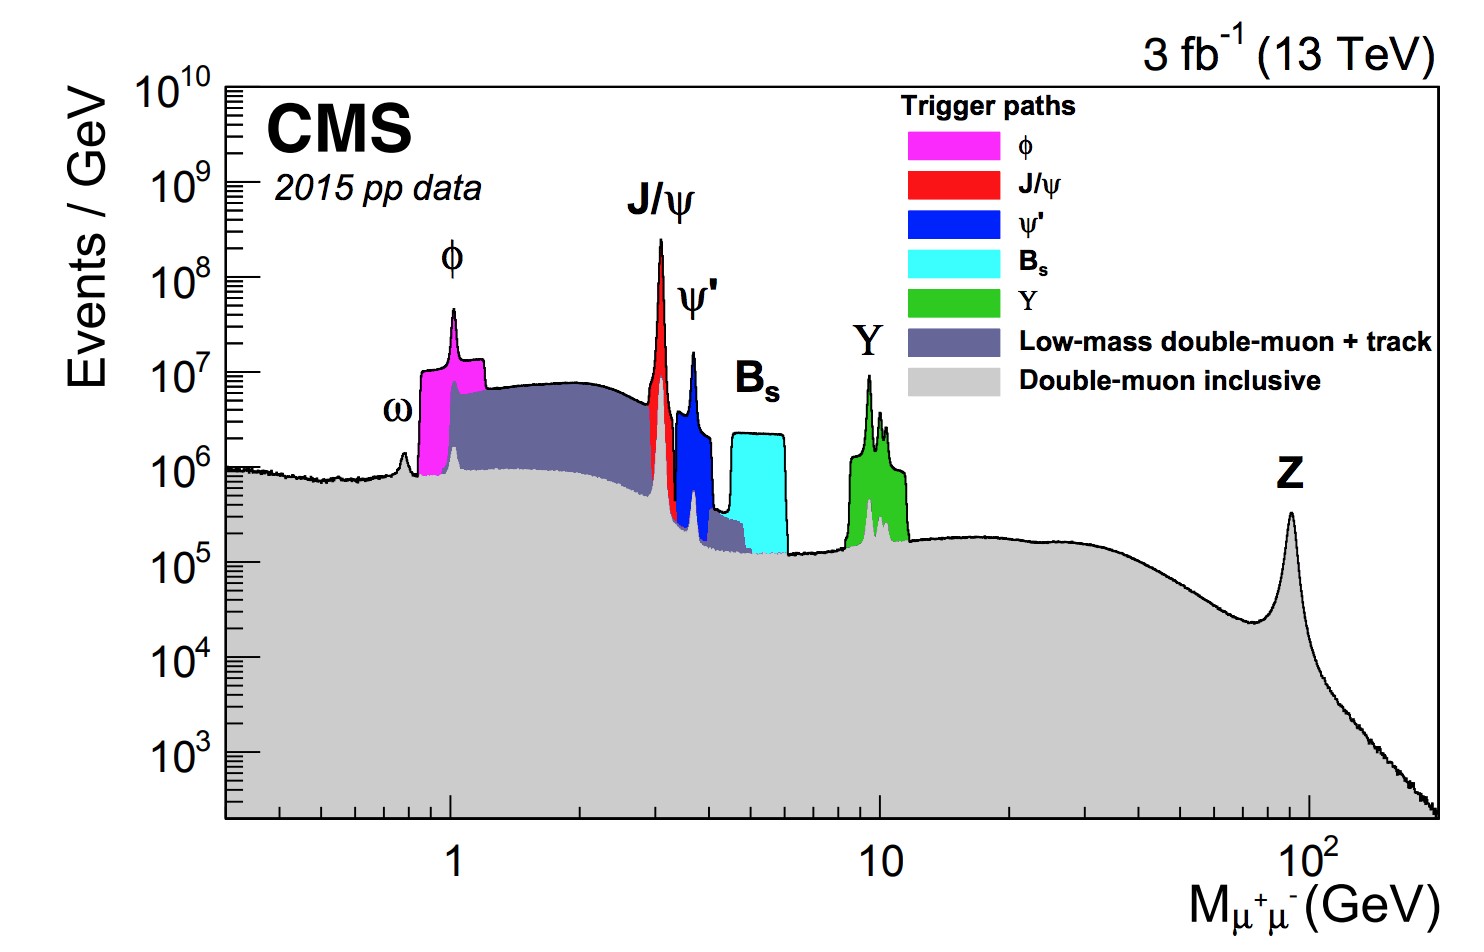
\includegraphics[width=.88\textwidth]{Figures/c2/dimuon}
\caption{``The dimuon invariant mass distribution reconstructed by the CMS HLT. Data were
collected in 2015 with the inclusive double-muon trigger algorithm (gray), as well as triggers
dedicated to selecting resonances at low masses.''~\cite{Sirunyan_2018_muon}.}
\label{fig:dimuon}
\end{figure}






\subsection{Track reconstruction} 
Electron reconstruction is based on the combination of tracker and
ECAL information in a Gaussian Sum Filter (GSF)
track~\cite{Khachatryan:2015hwa}, which accounts for possible
bremsstrahlung from the electron.
Electrons are reconstructed within the geometrical acceptance of the
CMS tracking system, $|\eta|<2.5$.
Identification criteria based on the electromagnetic shower shape, track
quality, track impact parameters with respect to the primary vertex,
and isolation are used to select signal electrons and reduce the rate
of mis-identified and background electrons (referred to as ``fake
electrons'' hereafter).

Muons are reconstructed by combining the information of the tracker
and of the muon
spectrometer~\cite{Sirunyan:2018fpa}.
The geometric compatibility between these separate measurements is
used in the further selection of muons. Muons are required to have
$\abseta<2.4$ to fall inside the geometric acceptance of the muon
detector.
All muons considered for analysis must pass the loose working point as
specified by the MUO POG, in addition to a number
of other loose criteria on isolation and their impact parameters with
respect to the PV.
It is also possible to require muons to be synchronized with the bunch
crossing that has triggered, using the time measurements provided by
the muon sub-detectors, the RPCs (``RPC time'' or $t_{\mathrm{RPC}}$)
and the combined measurements of the DTs and CSCs (``combined time''
or $t_{\mathrm{comb}}$)~\cite{muon_oot}.
In particular, $t_{\mathrm{RPC}}$ ($t_{\mathrm{comb}}$) is only used
if it is measured with more than 1 (7) degrees of freedom.
If $t_{\mathrm{RPC}}$ and $t_{\mathrm{comb}}$ are both available,
they must lie within $-10\ns$ and $+10\ns$.
If only $t_{\mathrm{comb}}$ is available, then it must be within
$-45\ns$ and $+20\ns$.
If $t_{\mathrm{comb}}$ is unavailable, no timing requirement is
applied.

\subsection{Reconstruction performances}
\clearpage
 
% Chapter Template

\part {Search for heavy neutral leptons}


\chapter{Heavy Neutral Leptons} 
\label{Chapter3} 


In the SM, all the fermions are known to have both left- and right-handed chirality, the only exception comes from the neutrinos.

The recent neutrino oscillation experiments have clearly and
definitely shown that neutrinos are massive.

The light masses of the SM neutrinos ($\nu_{SM}$) can be explained by introducing massive right-handed neutrinos ($\nu_{R}$), often referred to as \emph{heavy neutral leptons} (HNLs), via a type-I seesaw mechanism~\cite{MINKOWSKI1977421,gellmann2013complex,PhysRevLett.44.912,PhysRevD.22.2227}.
Another possible indication comes from the possibility to consider
$\nu_{R}$ as part of the explanation for the baryon asymmetry of the
universe; the $\nu_{R}$ mixing violates \emph{CP} symmetry and the $\nu_{R}$ interaction may potentially generate a matter-antimatter asymmetry in the early stage of the formation of the universe~\cite{Canetti_2012,KUZMIN198536}.

These few examples, which are going to be explored later on, already
show the relevance and the interest for the HNL search program, and
provide strong motivations to investigate the existence of the
$\nu_{R}$. This huge enthusiasm has led in the past $\sim10$ years to
the creation of a very active community with strong synergy between
theorists and experimental collaborations. It had contribute to the publication of an impressive numbers of papers and the proposal of a considerable number of experiments focused mainly on heavy neutral leptons. 

\section{Neutrino Portal} \label{sec:neutrinoPortal}
The \emph{neutrino portal} is defined as the coupling of one or more dark fermions $N_{I}$  ($I = 1,2,...$ $\mathcal{N}$), which are sterile with respect to the SM gauge interactions, to the gauge-invariant operator $\bar{L}_{\alpha}  \cdot \widetilde \Phi$; the general form of the neutrino portal could be written as: 
\begin{equation}
\label{eq:neutrinoportal}
\mathcal{L} = \mathcal{L}_{SM} + \mathcal{L}_{DS} + \sum F_{\alpha I} (\bar{L}_{\alpha}  \cdot \widetilde \Phi)N_{I} + h.c.
\end{equation}

where the summation loops over the flavor of lepton doublets
${L}_{\alpha}$ ($\alpha = e,\; \mu, \: \tau$) and the number of
available HNLs $N_{I}$; $F_{\alpha I} $ are the Yukawa couplings and
$\Phi$ is the Higgs doublet. The term $\mathcal{L}_{DS}$ is the dark
sector lagrangian which contains the mass term of HNLs which can be
either of Majorana or Dirac nature~\cite{Alekhin_2016}.
Fixing the $\Phi$ to its vacuum expectation value, $\widetilde \Phi = \frac{1}{\sqrt{2}} \binom{v}{0}$, and diagonalizing the mass term of the dark fermions, the last term in Eq.~\ref{eq:neutrinoportal} brings to the quadratic mixing of the neutrinos $\nu_{\alpha}$ with the $N_{I}$; this mixing is parametrized by a matrix $V$. In the minimal HNL models, the elements of the matrix $V$ control both the production and the decay of the HNLs. 
If $\mathcal{N} = 3$, there is a right-chiral counterpart for each $\nu_{SM}$, see Figure~\ref{fig:c3sm_extension}. The fermion $N_I$ can have mass $M_I$, which is independent  of the value of $F_{\alpha I}$.
\begin{figure}[t!]
  \centering
  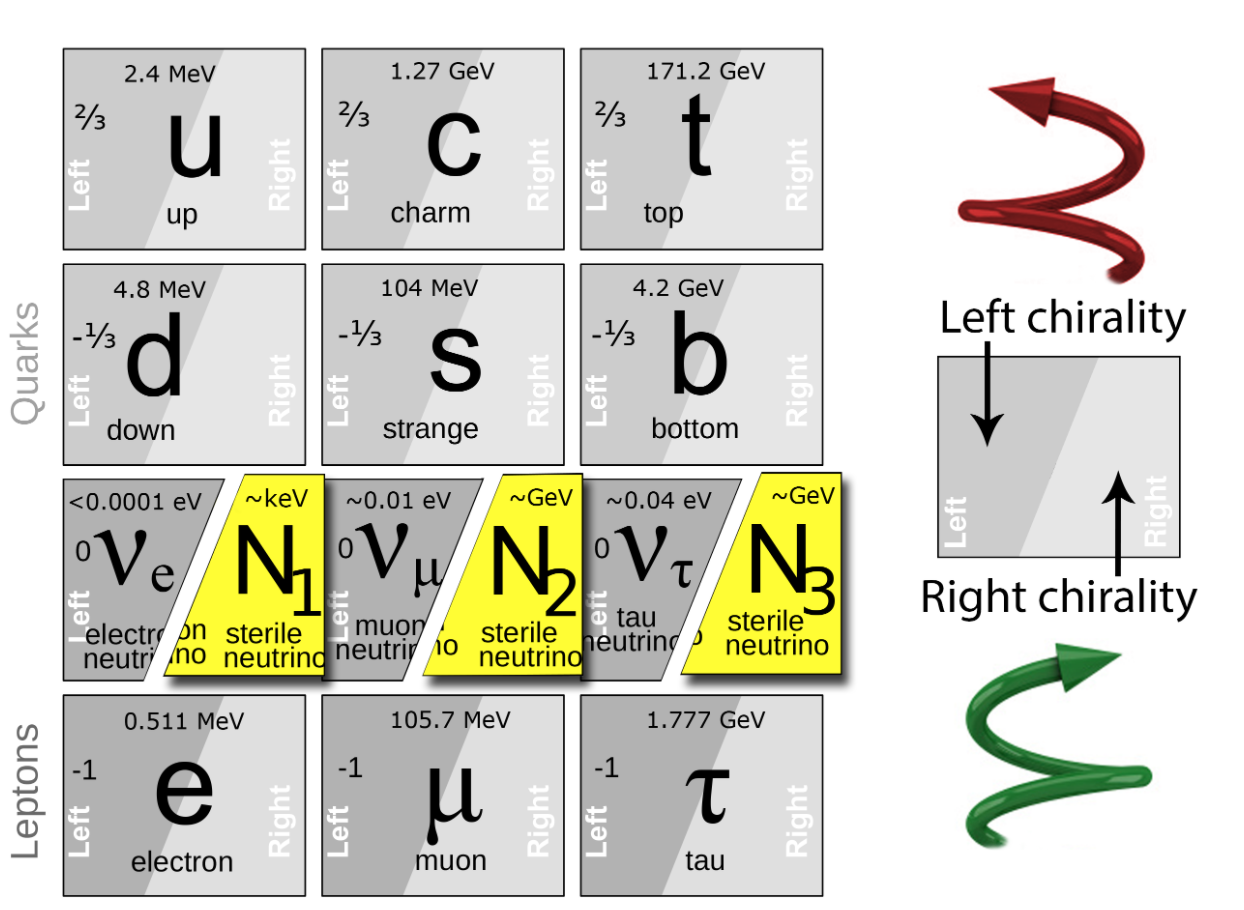
\includegraphics[width=.60\textwidth]{Figures/c3/SM_extension}
    \caption{There are 3 SM neutrinos $\nu_{e}, \; \nu_{\mu}, \;\nu_{\tau}$ which are massless and always left-chiral; 3 right-chiral counterparts are added $N_{1}, \; N_{2}, \;N_{3}$. They are sterile so they do not feel the electric, weak and strong forces. However they can be produced through mixing with the $\nu_{SM}$ with the corresponding mixing parameter.}
  \label{fig:c3sm_extension}
\end{figure}

Many HNL models require the existence of two or more right-handed neutrinos. In experimental searches, however, following a model-independent approach, we can consider the production of a \emph{single} HNL, which be light enough to be kinematically accessible at the accelerator experiments; see the full overview in~\cite{Atre_2009}. 

Under this assumption, there are then only two free parameters to be
constrained: the mass $M_I$ of the HNL and its mixing parameter with
the SM neutrino of flavor $\alpha$, controlled by the Yukawa coupling
$F_{\alpha I}$. The experimental sensitivity is expressed in terms of
the coupling $|V_{\alpha I}|^2$ ($= |F_{\alpha I}|^2$) as a function
of $M_I$ for a given flavor $\alpha$. It is frequently assumed that in
the matrix $V$ the other mixing elements for the residual flavors are
zero; although it does not translate into a valid concrete model, this latter consideration it is very useful to evaluate the experimental sensitivity on the single $|V_{\alpha I}|^2$ without involving any model dependent hierarchy between the different flavor mixings. 
%\begin{figure}[h]
%  \centering
%  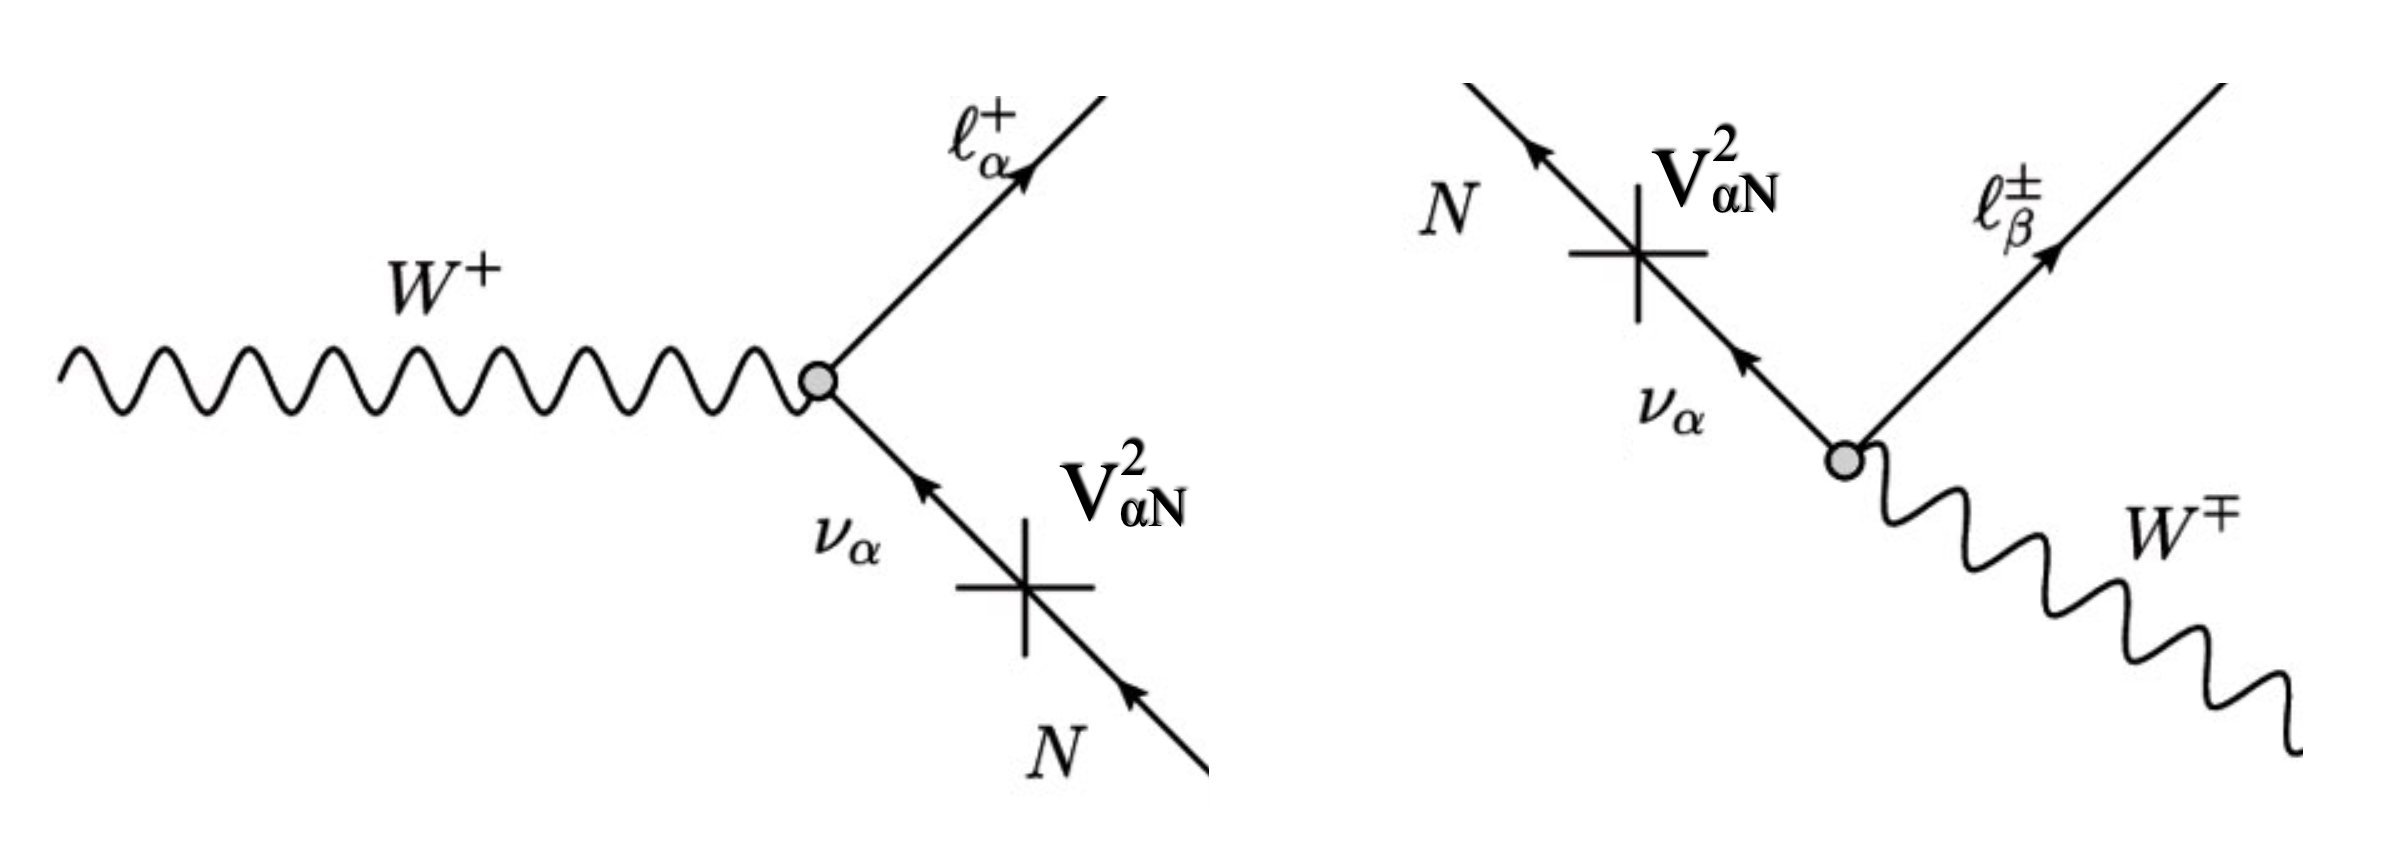
\includegraphics[width=.80\textwidth]{Figures/c3/diagram_decay}
%    \caption{Production (left) and decay (right) of the particle $N_{I}$.}
%  \label{fig:c3diagram_decay}
%\end{figure}

\section{Heavy neutral lepton formalism and extension of the Standard Model}
To set up our notation and conventions, we first discuss the formalism for the simplest
extension of the SM that includes right handed singlets. In section~\ref{sec:currentlimits}, we will try to contextualize the theory, explained here, summarizing the current constraints on the mass and mixing of a heavy neutrino from various direct
detection experiments, accelerator searches and electroweak precision
fits.

\subsection{Seesaw mechanism}\label{sec:seesaw}
The most general renormalizable Lagrangian for the neutrino masses includes both the Dirac and Majorana mass terms. The SM Lagrangian $\mathcal{L}_{SM}$ is extended adding $\mathcal{N}$ right-handed neutrinos $N_I$ (for notations see Eq.~\ref{eq:neutrinoportal}):
\begin{equation}
\label{eq:fullSMLag}
 \mathcal{L} = \mathcal{L}_{SM}+ i \bar N_I \partial_\mu \gamma^\mu N_I -
  \left(F_{\alpha I} \,\bar L_\alpha N_Is \tilde \phi 
    - \frac{M_I}{2} \; \bar {N_I^c} N_I + h.c.\right)
\end{equation}
As already explained in the section~\ref{sec:neutrinoPortal}, these $N_I$ are neutral with respect to all the gauge interactions of the SM, thus are called \emph{sterile neutrinos} or \emph{gauge-singlet fermions}.
In the Higgs phase, the term~\ref{eq:neutrinoportal} brings to the $\nu_{\alpha} - N_I$ mixing. As a result the \emph{charge eigenstates} of $\mathcal{L}_{SM}$ (Eq.~\ref{eq:fullSMLag}) do not coincide with \emph{mass eigenstates}, which can be extracted by diagonalizing the following matrix:
\begin{equation}
\label{eq:matrixmass}
 \mathcal{M}_{\nu,N} = 
\begin{pmatrix}
0 & m_D\\
m^{T}_{D} & M_I
\end{pmatrix}
\end{equation}
with the matrix elements defined as: $m_D = 3 \times  \mathcal{N}$ Dirac mass matrix, $(m_D)_{\alpha I} = F_{\alpha I}v, \; v = \sqrt{2}\langle \Phi \rangle$ and $M_I$ is $\mathcal{N} \times \mathcal{N}$ matrix of Majorana masses.

Considering the relation between $M_I$ and $m_D$, we could explore two interesting extreme limits:
\paragraph {Pure Majorana neutrino, $m_D \ll M_I$.}
In this limit, the mass matrix gives rise to 3 almost pure right-handed neutrinos with heavy Majorana mass $M_I$ and 3 almost pure left-handed neutrinos with light Majorna mass $m_\nu = - (vm_D)^{T}M^{-1}_{I}(vm_D)$ which are the 3 eigenvalues of the matrix $(\mathcal{M}_{\nu})_{\alpha \beta}$. This mechanism is then referred to as the \emph{seesaw mechanism}\footnote{This mechanism is usually called \emph{Type-I seesaw}. \emph{Type-II seesaw} has an extra SU(2) triplet scalar~\cite{Deppisch_2015}; in \emph{Type-III seesaw} an extra fermion in the adjoint of SU(2) is added to the model~\cite{Foot:1988aq}}~\cite{MINKOWSKI1977421}~\cite{Mohapatra:1979ia}~\cite{Yanagida:1979as}.
\begin{figure}[h]
  \centering
  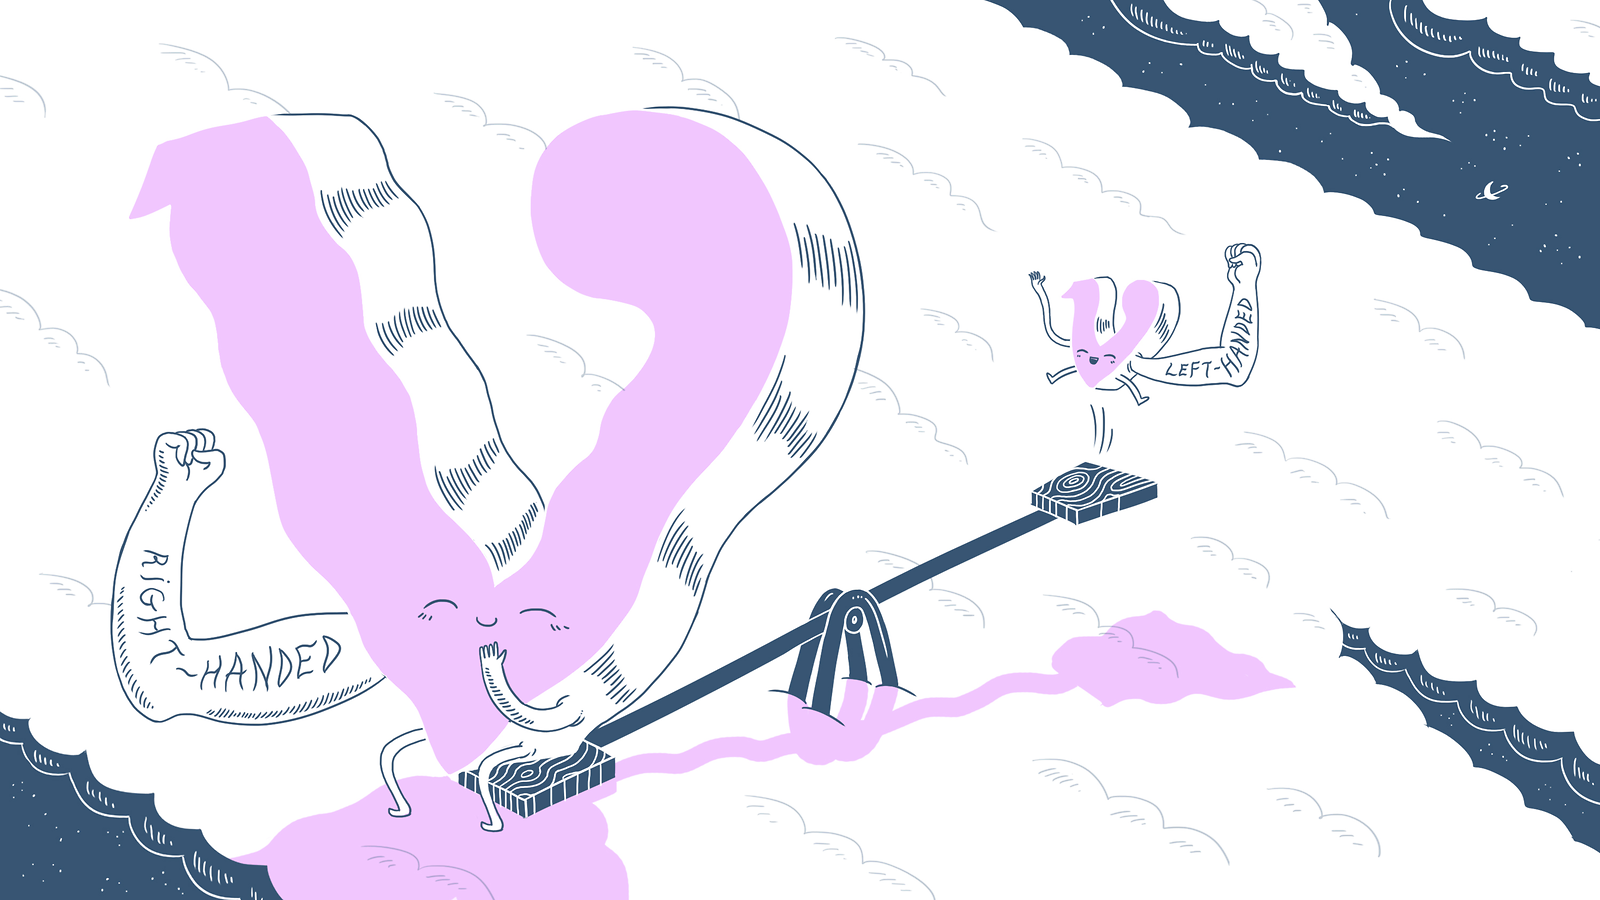
\includegraphics[width=.60\textwidth]{Figures/c3/funny.png}
    \caption{Silly representation of the \emph{seesaw mechanism}~\cite{funny}. Note that for a fixed value of $m_D$, the higher the value of the $m^{R}_I$ is, the lower $m^{L}_I$ is and vice-versa, from which we get the \emph{seesaw} name.}
  \label{fig:c3funny}
\end{figure}
There are then the other $\mathcal{N}$ eigenstates of the $\mathcal{M}_{\nu,N}$ which almost coincide with the $N_I$ up to a small admixture of $\nu_\alpha$.
The magnitude of this mixing is given by the ratio of the Dirac and Majorana masses, giving rise to the mixing angle or active-sterile mixing:

\begin{equation}
\label{eq:v2}
 |V_{\alpha I} |^{2}\equiv \frac{v^{2}|F_{\alpha I}|^2}{M^{2}_{I}} \ll 1
\end{equation}
%It generates the 9 measurable neutrino mass parameters from $m_D$ and $M_I$, that contain 18 unknown parameters to the Lagrangian: $number\; of \; HNL \; parameters = 7 \times \mathcal{N} - 3$. $\mathcal{N}$ are the real Majorana masses $M_I$ plus $3\times \mathcal{N}$ complex Yukawa coupling $F_{\alpha I}$ minus 3 phases which go to the redefinitions of $\nu_e, \; \nu_\mu,\; \nu_\tau$.

\paragraph {Pure Dirac neutrino, $M_I \ll m_D$.}
In this limit, the mass matrix gives rise to 3 Dirac neutrinos $\Psi = (\nu_L,\:\bar{\nu}_R)$ with masses $m_\nu = m_D$. To obtain the observed neutrino masses the coupling needs to be $F_{\alpha I} \sim 10^{-12}$ which is much smaller than the SM Yukawa couplings.

\subsection{Considerations on Majorana and Dirac neutrinos}\label{sec:c3majo_dirac}
The paragraphs below are freely inspired by the overview given by
R.D. Kauber in Ref.~\cite{webpage_seesaw}.
\subsubsection {Distinction between Majorana and Dirac terms.}\label{sec:majo_dirac}
The term \emph{Majorana} is used to define different properties and features and it is important for the following chapters to clarify the meaning.

In Section~\ref{sec:seesaw} \emph{Majorana} and \emph{Dirac} are used to
refer to the mass terms in the Lagrangian of Eq.~\ref{eq:fullSMLag}. An additional use is related to the type of neutrino. A \emph{Majorana} particle is defined as a particle that is its own antiparticle.  A Dirac particle has an antiparticle that is distinctly different from it.Neutrinos are the only particles that can be either \emph{Majorana} or \emph{Dirac}, while all the other known fermions were experimentally found to be of Dirac-type.

\subsubsection{Lepton Number conservation.}\label{sec:lnv_lnc}
To be clearer and explicit, we write the Dirac mass term as:
\begin{equation}
\label{eq:c3dirac}
-m_D (\bar{\nu}_L\nu_R + \bar{\nu}_R\nu_L)
\end{equation}
and the Majorana one:
\begin{equation}
\label{eq:c3majorana}
-\frac{1}{2}m^{L}_{I}(\bar{\nu}_L\nu^{c}_L + \bar{\nu}_L^{c}\nu_L) -\frac{1}{2}m^{R}_{I} (\bar{\nu}_R\nu^{c}_R + \bar{\nu}_R^{c}\nu_R)
\end{equation}
where R/L labels indicate the left- or right-hand chirality, and the
\emph{c} label the charge conjugation.

%In this way it is easier to see the interactions: $\nu_L$ destroys a left-handed (LH) neutrino and creates a right-handed (RH) $\bar{\nu}_R$, $\bar{\nu}_L$
% creates a LH neutrino and destroys a RH $\bar{\nu}_R$, $\nu^{c}_L$ creates a LH neutrino and destroys a RH antineutrino, $\bar{\nu}^{c}_L$ destroys a LH
 %neutrino and creates a right-handed antineutrino.

%Looking now at the Feynman diagram (right side of Figure~\ref{fig:c3hnldiagram}) of the first term of
%Eq.~\ref{eq:dirac} a RH particle disappears at a point and a LH
%particle appears. Therefore weak (chiral) charge is not conserved, but
%the lepton numbers is conserved, as we started with a
%neutrino (not an anti-neutrino) and ended up with a neutrino. \\
%Dirac neutrinos conserve the lepton number.

%Same considerations can be made for the Eq.~\ref{eq:majorana}, the
%weak charge is not conserved and neither the lepton number. We started
%with zero neutrinos and ended up with two neutrinos. \\
%Majorana neutrinos violate the lepton number.

Let us consider a HNL produced in the decay of a W boson, and its subsequent leptonic decays, as shown in Figure ~\ref{fig:c3hnldiagram}. If the HNL is of Majorana nature, then $\ell$ and l'$\ell^\prime$ (or $\ell$
and $\nu_{\ell^\prime}$) can either have the same chirality (Figure ~\ref{fig:c3hnldiagram} left) or opposite chirality (Figure ~\ref{fig:c3hnldiagram} right). The former decay represents a case of lepton-number violation (LNV), the latter a case of lepton-number conservation (LNC).

In the case of a HNL decay mediated by a $\PW^\ast$ boson, a LNV decay
(Figure~\ref{fig:c3hnldiagram} top left)
can lead to final states with no opposite-sign, same-flavor lepton
pairs (no-OSSF), such as $\Pe^\pm\Pe^\pm\PGm^\mp$ or
$\PGm^\pm\PGm^\pm\Pe^\mp$.
Decays mediated by a $\PZ^\ast$ boson (Figure~\ref{fig:c3hnldiagram}
bottom) and LNC decays (Figure~\ref{fig:c3hnldiagram} right), instead, are
always accompanied by an opposite-sign, same-flavor lepton pair
(OSSF).

The HNL can couple exclusively to a single lepton-neutrino family
(\ie only one of \mixpare, \mixparm, or \mixpart is nonzero)
or to multiple families (\ie at least two of \mixpare, \mixparm,
and \mixpart are nonzero at the same time).
In the former case, $\ell$ and $\ell^\prime$ (or
$\nu_{\ell^{\prime}}$) always belong to the same lepton family,
and the lepton flavor is conserved (LFC).
If \hnl couples to multiple lepton families instead, then the
lepton flavor can be violated, $\ell\neq\ell^\prime$ (LFV).
In the LFV case, decay rates to different flavors might not be the
same ($\mixpare,\mixparm,\mixpart>0$, but
$\mixpare\neq\mixparm\neq\mixpart$).

\begin{figure}
\centering
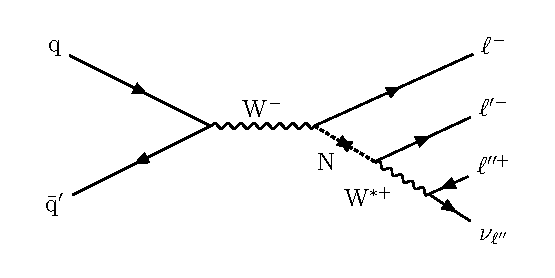
\includegraphics[width=0.45\textwidth]{Figures/c3/hnl_feyn.pdf}
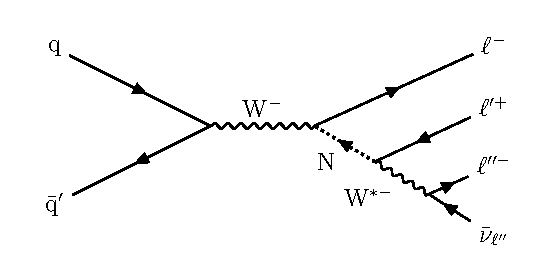
\includegraphics[width=0.45\textwidth]{Figures/c3/hnl_feyn_2.pdf}\\
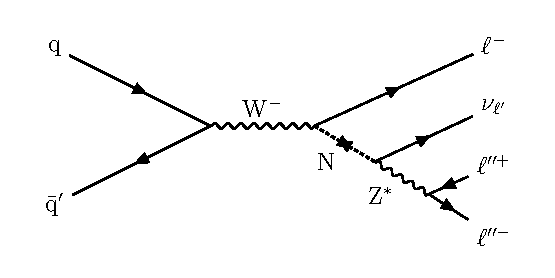
\includegraphics[width=0.45\textwidth]{Figures/c3/hnl_z_feyn.pdf}
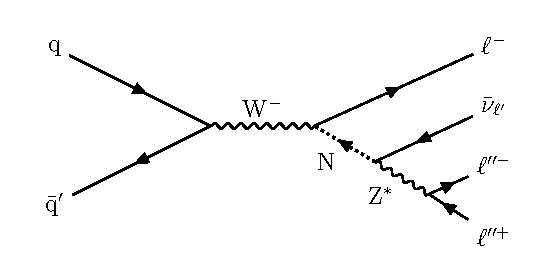
\includegraphics[width=0.45\textwidth]{Figures/c3/hnl_z_feyn_2.pdf}
\caption{Typical diagrams for the production of a HNL at the LHC 
($\hnl$) through its mixing with a SM neutrino, leading to a
final state with three charged leptons and a neutrino.
The HNL decay is mediated by either a $W$ (top row) or a $Z$ (bottom
row) boson.
In the diagrams on the left, $\hnl$ is assumed to be a Majorana
neutrino, thus $\ell$ and $\ell^\prime$ in the $W^\ast$-mediated
diagram (top) can have the same electric charge, with lepton-number
violation (LNV).
In the diagrams on the right instead, the $\hnl$ decay conserves the
lepton number (LNC) and can be either a Majorana or a Dirac
particle. Therefore $\ell$ and $\ell^\prime$ in the
$W^\ast$-mediated diagram (top right) have always opposite charge.
If \hnl couples exclusively to a single lepton-neutrino generation,
then $\ell$ and $\ell^\prime$ (or $\nu_{\ell^{\prime}}$) always belong
to the same lepton generation, and the lepton flavor is conserved
(LFC). If \hnl couples to multiple lepton families instead, then the
lepton flavor can be violated, $\ell\neq\ell^\prime$ (LFV).}
\label{fig:c3hnldiagram}
\end{figure}


\subsubsection{Decay width and branching ratio}\label{sec:decay_width}
The main consideration and difference between Majorana and Dirac HNL
is that in the first case the \hnl particle is defined as a particle
that is its own antiparticle. This implies that both $N_I\rightarrow
\PW^{+}\ell^-$, $\PZ\nu_{\ell}$, $H\nu_{\ell}$ and $N_I\rightarrow
\PW^{-}\ell^+$, $\PZ\bar{\nu}_{\ell}$, $H\bar{\nu}_{\ell}$ decay modes
are open. Assuming that the partial width of $N_I\rightarrow
\PW^{+}\ell^-$ and $N_I\rightarrow \PW^{-}\ell^+$ have the same
value, the total width for a Majorana neutrino and a Dirac
neutrino of same mass are related by:
\begin{equation}
\label{eq:width}
\Gamma^{Tot, \: Majorana}_{N_{I}} = 2 \times \Gamma^{Tot, \: Dirac}_{N_{I}}
\end{equation}
This leads to the following relationship between their lifetimes:
\begin{equation}
\label{eq:lifetime}
c\:\tau^{Tot, \: Majorana}_{N_{I}} = \frac{1}{2} \times c\:\tau^{Tot, \: Dirac}_{N_{I}}
\end{equation}

\subsection{Prompt and long-lived HNL}\label{sec:promptll}

The lifetime of a HNL is strongly dependent on $M_{N_I}$ and $|V_{\alpha I}|^2$,
and increases rapidly at small masses and low values of the mixing
parameter (see Figure~\ref{fig:hnlLifetime}):
\begin{equation}
\label{eq:lifetimedependences}
c\:\tau_{N_{I}} \propto\mathrm{M_{N_I}^{-5}|V_{\alpha I}|^{-2}}
\end{equation}
As a consequence, the kinematics and acceptance of HNLs with masses
below about 20 GeV are significantly affected by their long lifetimes,
and must be accounted for in the signal simulation and in the resulting
interpretation.
If $\hnl$ has a long lifetime, in particular, its decay products
($\ell^{\pm\prime}$, $\ell^{\mp\prime\prime}$, $\nu_{\ell^{\prime\prime}}$ or
$\nu_{\ell^{\prime}}$, $\ell^{\pm\prime\prime}$, $\ell^{\mp\prime\prime}$, see Figure~\ref{fig:c3hnldiagram})
emerge from a secondary vertex, spatially displaced with respect to
the primary vertex of the process, and distinguishable from it.
\begin{figure}
\centering
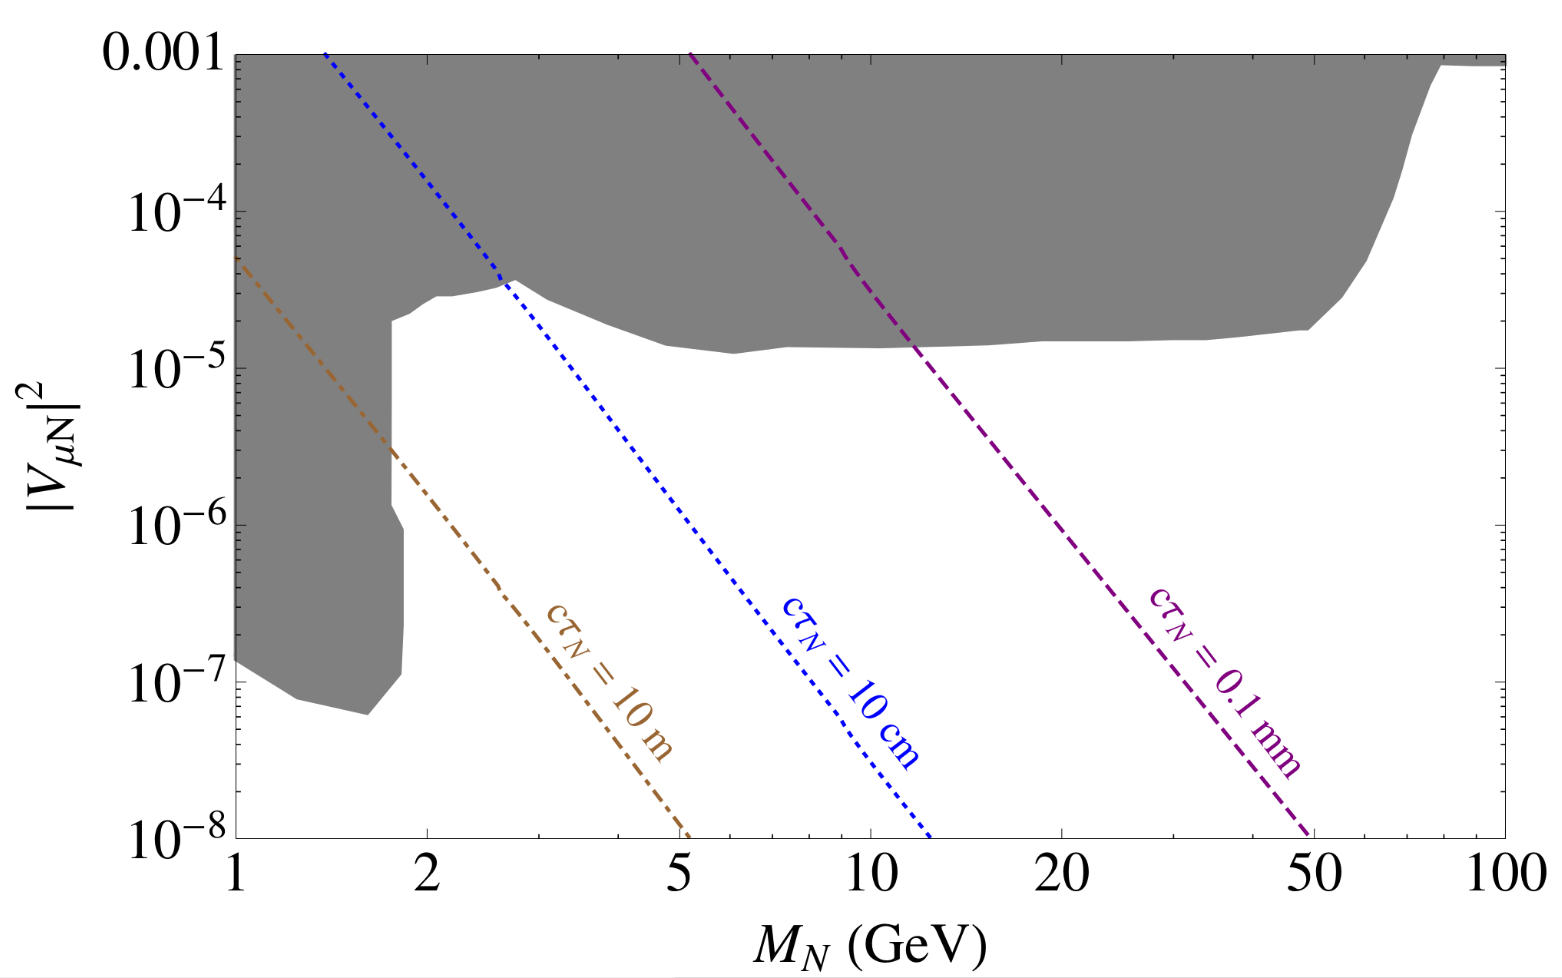
\includegraphics[clip,trim=0.cm 0.1cm 0cm 0cm, width=0.78\textwidth]{Figures/c3/graph_displ.png}
\caption{The calculated lines for $c\tau$ of a HNL are shown as a function of its mass \mhnl
and its mixing parameter \mixpar to a single lepton family:
the three oblique lines correspond to $c\tau$ values of (from left to
right) 10~m,  10~cm, and 0.1~mm.
The shaded grey area represents---approximately---the region of the
parameter space excluded by previous searches.}
%% If $\hnl$ has a long lifetime, its decay products emerge from a
%% secondary vertex, distinguishable from the primary vertex of the
%% process.}
\label{fig:hnlLifetime}
\end{figure}


%%%%%%%%%%%%%%%%%%%%%%%%%%%%%%%%%%%%%%%%%%%%%%%%%%%%
%%%%%%%%%%%%%%%%%%%%%%%%%%%%%%%%%%%%%%%%%%%%%%%%%%%%
%%%%%%%%%%%%%%%%%%%%%%%%%%%%%%%%%%%%%%%%%%%%%%%%%%%%
\section{Theoretical and experimental constraints} \label{sec:currentlimits}
For a complete overview of the theoretical and experimental constraints of sterile neutrinos searches see References~\cite{Deppisch_2015,10.3389/fphy.2018.00040,PhysRevD.78.013010,Drewes_2017,DREWES2017250,Antusch_2014}.


Sterile neutrinos mix with $\nu_{SM}$, thus at small mixing the
active-neutrino mass states contain a small part of sterile
neutrinos. Consequently, the mass eigenstates of the HNLs couple to SM
neutrinos thanks to the tiny, but nonzero mixing $V_{\alpha sI}$, Eq.~\ref{eq:v2}.

In principle, in any weak processes where $\nu_{SM}$ participate, the
HNLs also do so. The strength is suppressed due to the smallness of
the $\nu_\alpha - N_I$ mixing angle,
but the production of a HNL in the interaction can manifest itself in the kinematic properties of the final decay products, because HNLs are much more massive than active neutrinos.
Therefore, it is possible to select particular channels and phase spaces that enhance some kinematic features associated to the presence of the sterile neutrino.

These properties are explored and exploited in the direct searches for HNLs.



\subsection{Direct HNL searches}\label{sec:c3directHNL}
Considering the wide theoretically accessible mass ranges (MeV-TeV) and taking into account
the several production and decay modes, we have a quite rich
experimental landscape. 
\begin{itemize}
\item For $M_N$ values below 1 MeV, HNL can be probed by
  neutrino-oscillation experiments~\cite{de_Gouv_a_2005};
\item for 10 eV $< M_N <$ 1 MeV, searches for neutrinoless double-beta decay,
  $0\nu\beta\beta$ and precision measurements of $\beta-$decay energy
  spectra have constrained the mixing \mixpare, only for Majorana cases~\cite{Deppisch_2015};
\item for 1 MeV $< M_N <$ 1 GeV, both \mixpare and \mixparm have been
  constrained by peak searches using leptonic decays of pions
  and kaons like $K \rightarrow \mu(e) N$, $\pi \rightarrow \mu(e)
  N$~\cite{Liventsev_2013};
\item for HNL in the MeV-GeV mass ranges, many searches through
  sterile neutrino decay products have been performed at beam-dump experiments~\cite{DORENBOSCH1986473};
\item for HNL in the GeV-TeV mass ranges, we enter the domain of
  the particle colliders.
\end{itemize}

Quite often the HNL bounds are shown in the 2D $V_{\alpha N} -
M_N$ plane for a specific mixing parameter V, under the assumption that all the other mixing angles are zero. 

To have a clear overview of the current experimental (and theoretical)
limits we can refer to
Figs.~\ref{fig:HNL_bc6_pbc_2},~\ref{fig:HNL_bc7_pbc_2}
and~\ref{fig:HNL_bc8_pbc_2}. Filled colored areas show the existing limits. For HNL masses below the charm mass, the limits are driven by the results from beam-dump experiments (PS191 and CHARM); for masses above
the charm mass, the most stringent limits are those coming from LEP experiments
(especially DELPHI), from Belle, and, more recently, from CMS and ATLAS.



\begin{figure}[h]
  \centering
  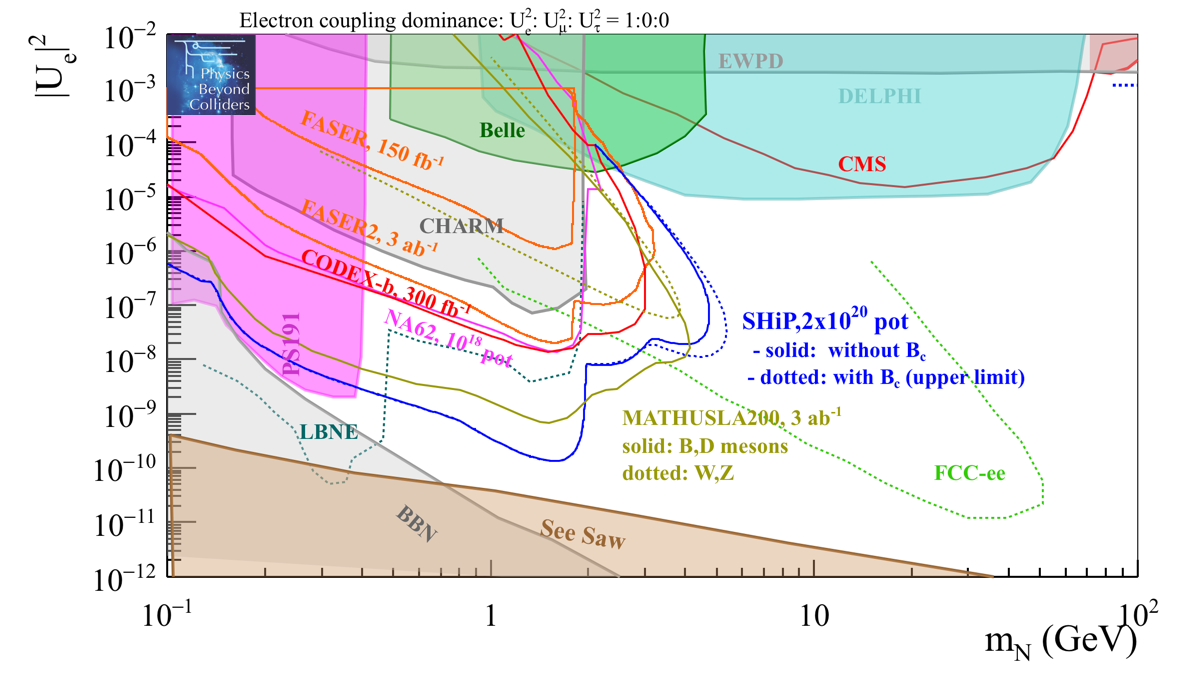
\includegraphics[width=.90\textwidth]{Figures/c3/HNL_bc6_pbc_2.png}
    \caption{Sensitivity to HNL with coupling to $\nu_e$ only. Current bounds (filled areas) and 10-15 years prospects for projects
(SHiP, MATHUSLA200, CODEX-b and FASER2) (solid lines). Projections for a LBNE
near detector with $5\times 10^{21}$ protons-on-target and from FCC-ee with
$10^{12}$ $\PZ_0$ decays are also shown.
The gray contour named "BBN'' corresponds to a HNL lifetime $>1$sec,
which is disfavored by BBN~\cite{Ruchayskiy_2012}. The brown line
labeled "seesaw'' represents the scale of mixing in general expected
in the canonical seesaw. The very light gray at the top
labeled as "EWPD'' is the 90\% C.L. exclusion limit from the
electroweak precision data~\cite{Antusch_2015}. The other solid
contours are explained in the text. 
% The green contour labeled "Belle'' is the exclusion
%region at 90\% C.L from HNL searches in B-meson decays at
%Belle~\cite{Liventsev_2013}. Those labeled "PS191'' (magenta) and
%"CHARM' (gray) are excluded at 90\% C.L. from beam-dump experiments.
}
  \label{fig:HNL_bc6_pbc_2}
\end{figure}

\begin{figure}[h]
  \centering
  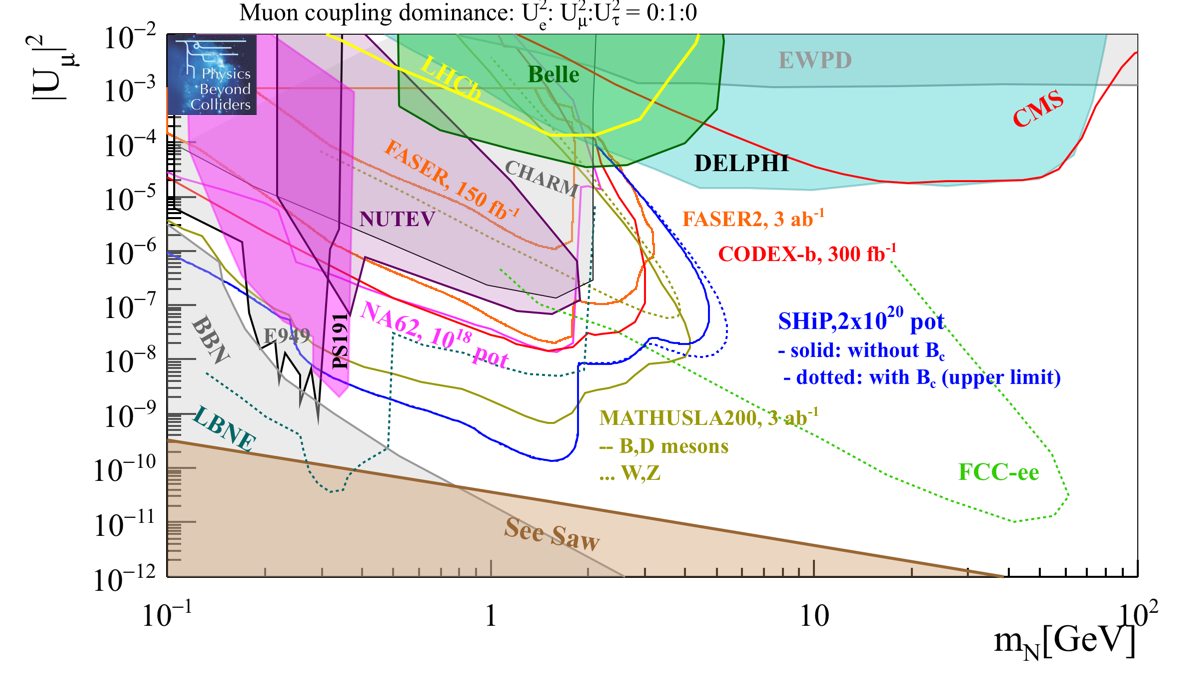
\includegraphics[width=.90\textwidth]{Figures/c3/HNL_bc7_pbc_2.png}
    \caption{Sensitivity to HNL with coupling to $\nu_\mu$ only. Current bounds (filled areas) and 10-15 years prospects for projects
(SHiP, MATHUSLA200, CODEX-b and FASER2) (solid lines). Projections for a LBNE
near detector with $5\times 10^{21}$ protons-on-target and from FCC-ee with $10^{12}$ $\PZ_0$ decays are also shown. The gray contour named "BBN'' corresponds to a HNL lifetime $>1$sec,
which is disfavored by BBN~\cite{Ruchayskiy_2012}. The brown line
labeled "seesaw'' represents the scale of mixing in general expected
in the canonical seesaw. The very light gray at the top
labeled as "EWPD'' is the 90\% C.L. exclusion limit from the
electroweak precision data~\cite{Antusch_2015}. The other solid
contours are explained in the text.}
  \label{fig:HNL_bc7_pbc_2}
\end{figure}

\begin{figure}[h]
  \centering
  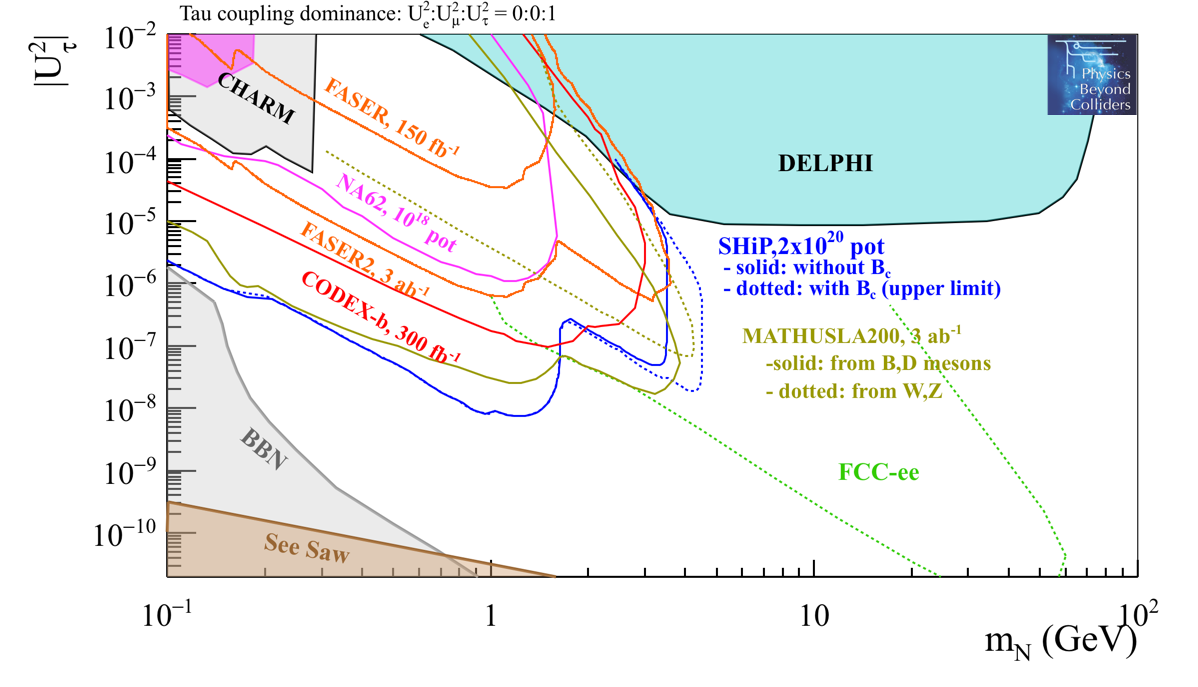
\includegraphics[width=.90\textwidth]{Figures/c3/HNL_bc8_pbc_2.png}
    \caption{Sensitivity to HNLs with coupling to $\nu_\tau$ only. Current bounds (filled areas) and 10-15 years prospects for projects
(SHiP, MATHUSLA200, CODEX-b and FASER2) (solid lines). Projections from FCC-ee with $10^{12}$ $\PZ_0$ decays are also shown.}
  \label{fig:HNL_bc8_pbc_2}
\end{figure}

A brief experiment-focused overview follows:
\begin{itemize}
\item \textbf{PS191} (CERN, PS Beam 1983)~\cite{BERNARDI1988332}: the PS191
  experiment was specifically designed to look for neutrino decays in
  low-energy neutrino beams. It was a detector composed of a 12 m long
  decay volume followed by a fine-grain calorimeter. No sterile
  neutrino candidates were observed but the analysis of neutrino
  interactions in the calorimeter shows a possible excess of events
  with electrons~\cite{Vannucci:1985vs}.
\item \textbf{CHARM} (CERN, SPS beam 1985)~\cite{DORENBOSCH1986473}: a search
  for HNL decays  was performed by the CHARM Collaboration using a
  neutrino beam produced by dumping 400 GeV protons on a thick Copper
  target and looking for possible visible decays. The sterile neutrino was assumed to be produced in charmed D meson decays, \ie $c\rightarrow s W^{*}$ with $W^{*} \rightarrow \ell \hnl$. The following decays were considered, \hnl $\rightarrow
  e^+e^-\nu_e$, $\rightarrow \mu^+e^-\nu_\mu$ and $\rightarrow
  \mu^+\mu^-\nu_\mu$ and the limits were set on \mixpare and
  \mixparm $< \:10^{-7}$ for \hnl masses around 1.5 GeV. 
\item \textbf{Belle} (KEK, asymmetric-energy $e^+e^-$ collider, 2012)~\cite{Liventsev_2013}: the Belle Collaboration
  performed a search for heavy neutral leptons in B-meson
  decays. The data sample contained $772\times 10^6$ $B\overline{B}$
  pairs collected at the $\Upsilon(4S)$ resonance. The limits
  on the mixing parameter were obtained analyzing the $B\overline{B}$ pairs
  events using the leptonic and semileptonic B meson decay,
  $B\rightarrow X\ell\nu_R$, where $\ell = e, \: \mu$ and the $X$ was
  either a charmed D meson, a light meson ($\pi, \: \rho, \: \eta$) or
  nothing (leptonic decay). Upper limits were set on \mixpare and
  \mixparm in the mass range 0.5--5.0 GeV. 
\item \textbf{DELPHI} (CERN, lepton collider LEP, 1997)~\cite{Abreu:1996pa}:
  up to the publication of the results presented in this thesis, the most stringent limits between 1 GeV and 10 GeV have been those published by the DELPHI Collaboration. HNL searches were performed
  using the data collected by DELPHI, corresponding to $3.3
  \times 10^6$ hadronic $Z_0$ decays at LEP1. This set of results is, up to
  this day, one of the most complete, including both the short-lived HNL and the long-lived
  HNL scenario and all three lepton flavor couplings. 
  According to the mass and lifetime ranges of the HNL, four separate searches were performed, two for short-lived \hnl production giving monojet or acollinear jet topologies, 
  and two for long-lived \hnl looking for detectable secondary vertices or calorimeter clusters.
 Upper limits were set for the branching ratio $BR (\: Z_0\rightarrow$ \hnl) of
 about $1.3 \times 10^{-6}$ at 95\% C.L. for \hnl masses between 1 and
 80\GeV. An additional combination of the short and long lived HNL searches was performed providing the upper limits on \mixpar for \hnl masses between 3.5 and
 50\GeV. 
\item \textbf{CMS and ATLAS} (CERN, LHC pp beam, 2019): there have been several searches for HNLs in both CMS and ATLAS.
The ATLAS experiment recently reported on a search for HNLs using events with three charged leptons~\cite{atlasintro2} using 
pp collisions data corresponding to integrated luminosities of 32.9 to
36.1 $fb^{-1}$. 
The search is performed in channels with three muons or two muons plus
one electron---providing sensitivity  to \mixparm only---, where the 
displaced decay vertex of the HNL was exploited.
CMS performed searches for HNLs only using prompt leptons,
either in final states with two same-charge leptons and one or two jets
(\(\PW^{\pm(\ast)}\to\ell^{\pm}\hnl\to\ell^{\pm}\ell^{\prime\pm}q\bar{q}^{\prime}\))~\cite{Sirunyan:2018xiv},
or in final states with three prompt leptons and \ptmiss 
in a mass range of 20 GeV to 1.7 TeV.
CMS searches with three charged leptons in the final state using the leptonic \PW decay are going to be extensively discussed in this
dissertation.
\end{itemize}

\subsection{Theoretical constraints on HNL}
In the following list, we tried so summarize the current constraints
coming from theoretical predictions and from the most recent results (Figs.~\ref{fig:HNL_bc6_pbc_2},~\ref{fig:HNL_bc7_pbc_2}
and~\ref{fig:HNL_bc8_pbc_2}.)
\begin{itemize}
\item \textbf{Searches for Charged Lepton Flavor Violation}. If we consider a HNL with a
  mass close to the EW scale and with large off-diagonal Yukawa couplings,
  then this can lead to LFV in decays of charged leptons. Thus,
  testing LFV in multi-lepton searches could be an indirect way to
  probe the existence of HNL. Searches for such processes have
  placed 90\% C.L. upper limits on decay branching rates, \ie
  $BR(\mu^+\rightarrow e^+\gamma) < 4.2\times 10^{-13}$,
  $BR(\mu^+\rightarrow e^+e^+e^-) < 1.0\times 10^{-12}$ and
  $BR(\tau^-\rightarrow e^-\mu^+\mu^-) < 2.7\times 10^{-8}$. For a 
  complete summary and references see~\cite{Pascoli_2019}.
\item \textbf{Cosmological constraints on light neutrino masses}. The Planck
  Satellite's measurements of the large scale structures in the
  universe, combined with the WMAP + highL + BAO data, have set the
  upper limits on the sum of all the light
  neutrinos~\cite{Aghanim:2018eyx}.
\begin{equation}
\label{eq:summasses}
\sum_{m} m_{\nu_m} < 0.12 \: eV, \;\;\;\; at \;95\% \: C.L.
\end{equation}
This upper limit on the active neutrino masses is directly connected
with the possibility of the existence of HNLs and with the predicted
numbers of \hnl, $\mathcal{N}$.
If the seesaw mechanism is assumed to be responsible for the origin of neutrino masses,
one RH neutrino is necessary per observed nonzero light
neutrino mass~\cite{Alekhin_2016}.
To conclude, the interpretation of direct search experiments limits and cosmological constraint both strongly
depend on $\mathcal{N}$ and the $\nu_{SM}$
mass~\cite{DREWES2017250,drewes2015theoretical}. To clarify, for
$\mathcal{N}=3$, if the lightest neutrino is massless, no
lower bound on the mixing parameter \mixpar can be set.
On the other hand, if it is the case like in Eq.~\ref{eq:summasses}, then there is a lower
bound on \mixpar~\cite{DREWES2017250}.
\item \textbf{BBN constraints}. Observing
  Figs.~\ref{fig:HNL_bc6_pbc_2},~\ref{fig:HNL_bc7_pbc_2}
  and~\ref{fig:HNL_bc8_pbc_2}, a HNL that falls on the left of the
  Big Bang Nucleosynthesis line would live long enough in
  the early universe to cause an overproduction of primordial
  Helium-4~\cite{Ruchayskiy_2012}.
\item \textbf{Seesaw limit}. Below the line of the seesaw limit, the
  mixing of the sterile neutrinos with the active ones becomes too
  weak to be able to produce the pattern of neutrino flavor oscillations that has been observed~\cite{Canetti_2010}. 
\end{itemize}
\clearpage
\section{Summary}
In this chapter we illustrate the relevance and the enthusiasm in the
current HNL search program, describing first the theory setting of RH
neutrinos and then reporting the rich plethora of experiments and results
focusing on HNL.\\
In the SM, all fermions are known to have both
left- and right-handed chirality, the only exception comes from 
neutrinos. One argument in favor of the introduction of massive RH
neutrinos is that they give an answer to the SM problem of the
neutrino masses via seesaw mechanism. The neutrino mass
problem is one of the open questions in physics that indicates that
other fundamental physics remains to be unmasked.

When we hypothesize RH neutrinos, $N_{I}$, as new particle on the SM we
are interested in their properties like the mass $M_I$ and
their mixing parameter, $|V_{\alpha I}|^2$,  with the SM neutrino of flavor $\alpha$,
controlled by the Yukawa coupling $F_{\alpha I}$. The values of $|V_{I
  \alpha}|^2$ are unknown and usually the experimental
sensitivity is expressed in terms of the coupling $|V_{\alpha I}|^2$
as a function of $M_I$ for a given flavor
$\alpha$.

A list of direct HNL search results are presented; we give an overview
of the experimental current and past landscape describing the different decay modes and
mass ranges that are targeted by each experimental setup.
The strategies in direct HNL searches depend greatly on the coupling
and mass of the HNLs. For $M_{I} > 5$\GeV, \hnl can be
produced uniquely at either LHC or at similar energy colliders, via a few
mechanisms (vector boson fusion, s-channel exchange of virtual
W-bosons or in real gauge boson decays) according to the production
energy and \hnl mass. A more extensive explanation is given in the following
Chapter~\ref{Chapter4}. For $M_{I} < 5$\GeV, we turn to b-factories
or fixed target experiments. \\
In this chapter, special attention is paid to lepton and hadron collider
searches. The LEP results from DELPHI happen to be the best results at
low mass from collider experiments up to the publication of the results
of this dissertation. For the author, the outstanding sensitivity at low mass from
$e^{+}e^{-}$ data was surely a good motivation to invest a quite
important effort to extend the low mass sensitivity of
the CMS experiment. Chronologically we have focused first on the
moderate and high mass search to then migrate to the very low mass search which
necessarily requires the inclusion of displaced scenarios.

Finally an overview of the theoretical HNL
constraints is presented.\\
Taking into account 
the current experimental and theoretical limits on the HNL
mass, we discussed the allowed mass window of sixteen orders of magnitude
$100\ \MeV < M_{I} < 1\ \TeV$. This clearly necessitates to adopt a
comprehensive and vast approach in seeking for HNL.
The very wide range of masses, energies and models expects to
explore the complementary reach of the current and future experiments.\\





%\begin{figure}[t!]
%  \centering
%  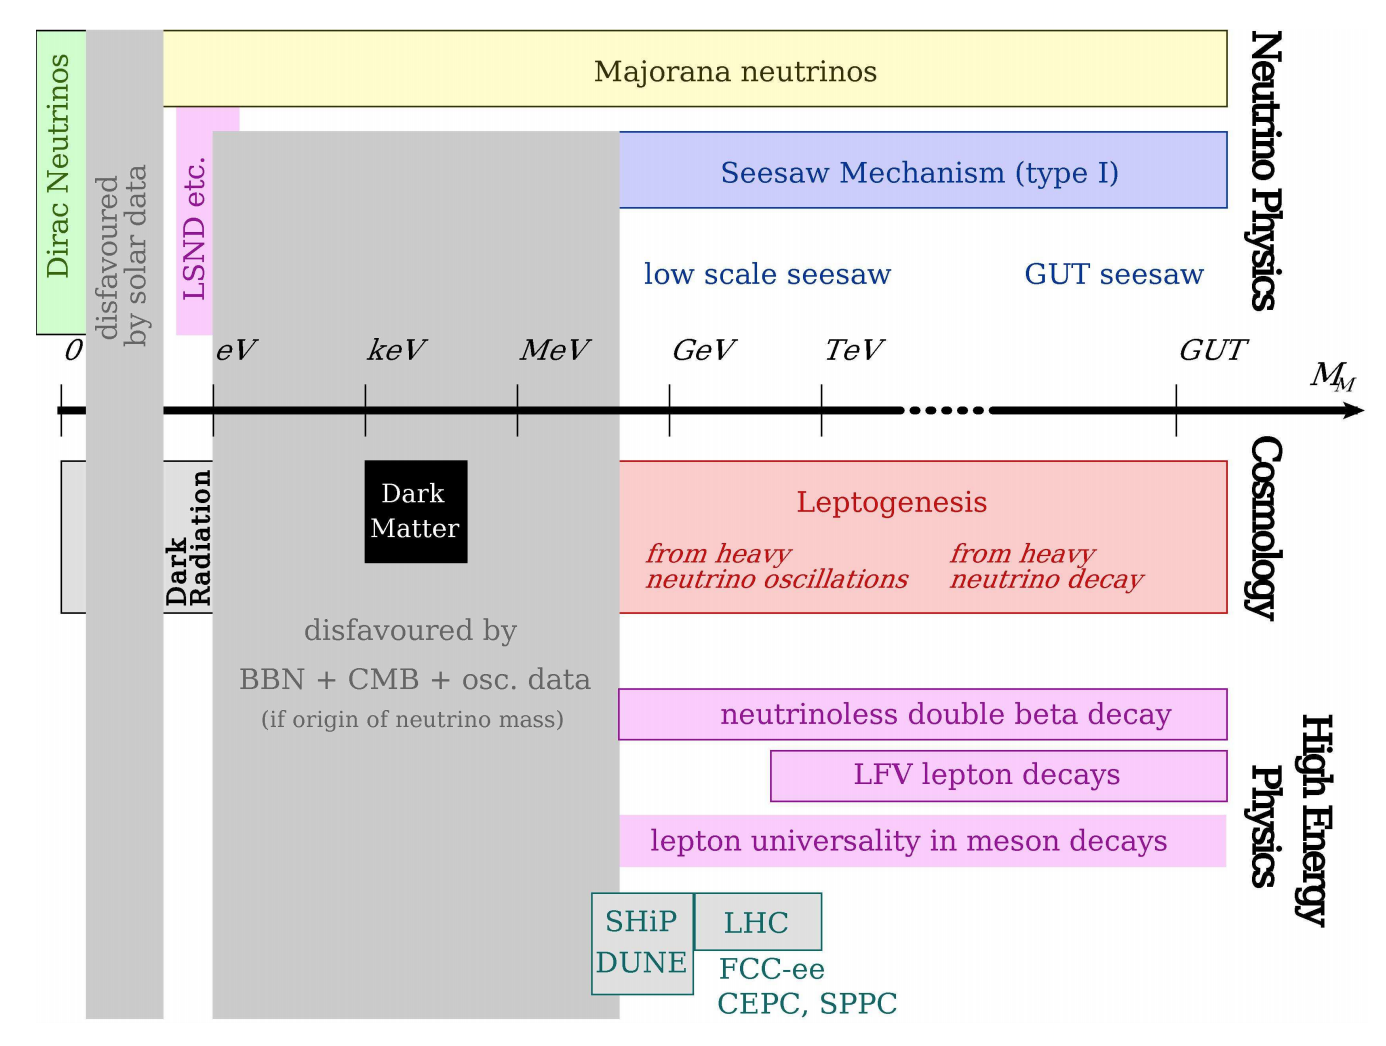
\includegraphics[width=.99\textwidth]{Figures/c3/marcoscheme.png}
 %   \caption{A schematic overview from Reference~\cite{DREWES2017250}
 %   ``of the allowed range of values for the “seesaw scale” and their
 %   implications for neutrino physics, cosmology and high energy physics''.~\cite{DREWES2017250}}
 % \label{fig:marcoscheme}
%\end{figure}







% Chapter Template
\chapter{Data and simulated datasets} \label{Chapter4} 


Nearly all of new physics signals which can be studied at CMS are
expected to have their potential backgrounds in which SM
processes sporadically have fluctuations that make them appear more
exotic than they truly are, or backgrounds arising from detector noise
or mis-measurements.
For example, an isolated high \pt electron can be a ``smoking gun'' for
a few rare new physics processes. At the same time an electron contained in a b
jet is hardly ever isolated, but since the total b jet cross section
is extremely large, even a small portion can be critical. It becomes
crucial to have a sort of ``litmus test'' to cross-check the observed
outcomes with the expected features and the predicted amount of events.
The idea is to validate the observed information by comparing it to
generated events. For this reason collision events are simulated for
several physics processes as they are predicted from theory. The
detector simulation response is taken into account. \\
In a simplistic way we can summarize a number of applications of event
generators as follows: to give analyzers a sense of the type of
events to expect and at which rates; to help in planning new
experiment designs hence detector performances are optimal for the
desired physics search; to help in drafting analysis strategies which
can be applied to data but that have been optimized a priori without
any possible unconscious bias; to estimate detector calibrations and acceptance
corrections; and to have a appropriate framework inside which to
interpret the meaning of observed physics phenomena in the optics of a
fundamental underlying theory (SM).



\section{Simulation of pp collision events}\label{sec:c4eventsimulation}

The event simulation is based on the Monte Carlo (MC)
method~\cite{mc}. The simulated events
 are grouped in a specific
sample for each physics process and they are called MC samples.\\
The full simulation chain is divided in separate generation stages:
\begin{itemize}
\setlength\itemsep{-0.1em}
\item \textbf{Matrix element (ME) calculation.} The ME calculation
  makes use of a list of PDFs (Parton Distribution Function) for the initial state
  depiction; a MC generator is used for the computation of the
  partonic interaction.
 For the signal samples produced specifically for this thesis and for
  most SM processes here presented, the software
  \texttt{MadGraph5\_aMC@NLO}~\cite{Alwall_2014} is used. For a few other background processes 
  the \texttt{POWHEG}~\cite{Alioli_2010} software is used. Both
  softwares have LO and NLO accuracy in QCD. For proton PDFs, in both
  generators, the NNPDF3.0~\cite{Ball_2015} and
  NNPDF3.1~\cite{Ball_2017} PDFs are used as input.
\item \textbf{Parton shower simulation.} The simulation is done with
  the \texttt{PYTHIA 8}~\cite{Sj_strand_2008, Sj_strand_2015}
  software. The parton shower step is necessary to address some aspects
  of the collision with regards to the evolution of quarks and gluons into jets of
  hadrons, so called \emph{hadronization}. The hadronization is
  simulated starting from an energy scale of 1 GeV, adopting phenomenological models tuned to
  experimental results~\cite{Skands_2014, Khachatryan_2016_ps, Sirunyan_2020_ps}.
\item \textbf{Detector simulation.} The detector simulation is done
  with \texttt{GEANT4}~\cite{AGOSTINELLI2003250} software. The
  simulation is based on an accurate geometrical model of the CMS
  detector, hence it includes all the material budget and it tracks
  the authentic sub-detector responses. Particle interactions with
  matter are simulated and their energy deposit is reproduced according to the
  energy and the mass of the particle and the material that it goes through. Data collected by CMS are used to
  parametrize the real detector response of each single
  sub-detector. Furthermore the trigger system and the readout system
  is mimicked. 
\end{itemize}

While analyzing the simulated samples the kinematics and all
properties of the produced primary particles are available in addition
to the detector signals just like in real collision data. This
possibility makes the simulations a corner stone of the detector and
algorithm performance studies.\\
Furthermore there are single year campaigns for
each year of data-taking which correspond to different detector
conditions for each period. 



\section{Standard Model processes}\label{sec:c4sm}
\begin{figure}[h]
\centering
  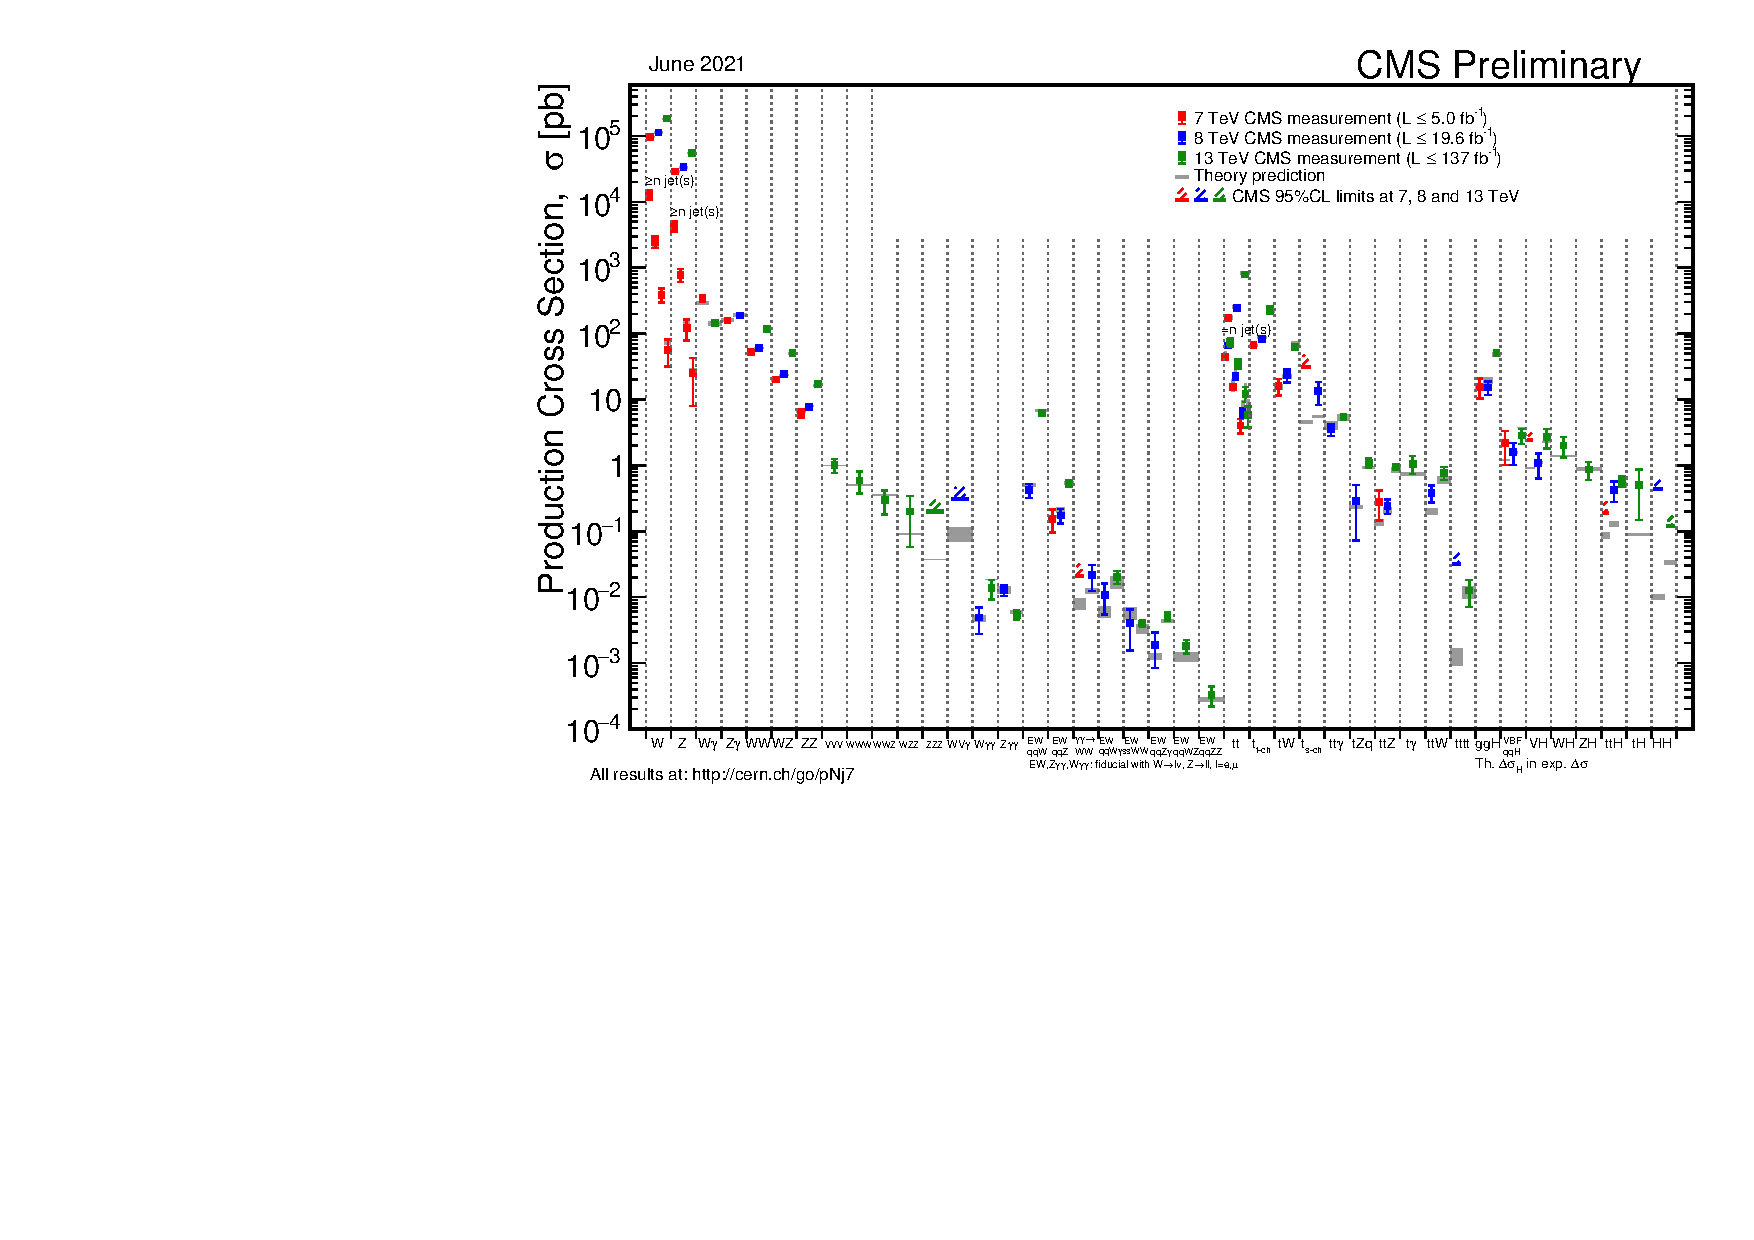
\includegraphics[width=0.85\textwidth]{Figures/c4/SigmaNew_v0.pdf}
  \caption{Summaries of cross sections measurements by CMS~\cite{cmspublic} for
    different center-of-mass energies compared to the theory
    predictions (gray). The plot gives hints about the
    amount of events we could expect from each single process and the
    relative rates with respect the signal expected yields.}
  \label{fig:crosssection}
\end{figure}
In this section we give an overview of the SM processes that form
sizable backgrounds to the HNL searches performed in this thesis. The
focus is specifically on processes that can lead to three light
lepton final states, which is the
signature given by HNL decaying either into \PZ or into \PW where the bosons
decay leptonically; this final state is presented in
Chapters~\ref{Chapter5} and~\ref{Chapter6}.

In Figure~\ref{fig:crosssection} a summary of cross sections
measurements by CMS is presented. The measured values are compared
with the theory predictions showing outstanding agreements.

Almost all of the backgrounds are estimated from simulation using the
MC samples. The nonprompt lepton background is the only exception and it is
discussed for each analysis separately in Sections~\ref{sec:tight_loose_method}
and~\ref{sec_llfakelepton}. 

In the next paragraphs the SM processes that contribute the most as 
backgrounds to the HNL searches are listed and explained.

\paragraph{WZ and ZZ production}\label{sec:c4wz_zz}
In case both bosons decay leptonically, the associated production of
WZ bosons produces three prompt leptons ($\PZ \rightarrow \ell^{+}
\ell^{-}$, $\PW \rightarrow \ell \nu$) and \ptmiss.
Its clear signature is an opposite sign same flavor (OSSF) pair with
invariant mass compatible with \PZ mass. The events are characterized by
having a few jets or none, and zero b jets.
WZ events
constitute a dominant background in the three prompt leptons HNL
analysis presented in Chapter~\ref{Chapter5}.

\begin{figure}[h!]
\centering
  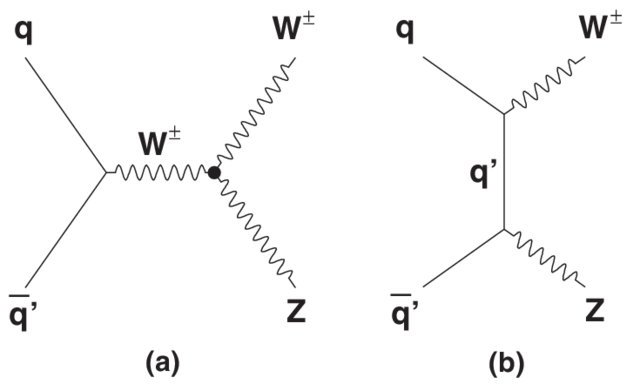
\includegraphics[clip,trim=0.cm 0.5cm 0cm 0cm, height =2.5cm]{Figures/c4/dia/wz.jpeg}\\
  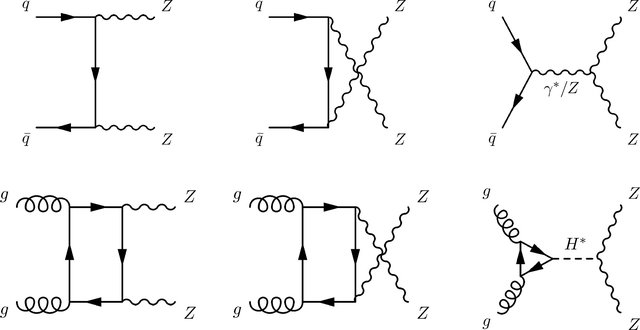
\includegraphics[clip,trim=0.cm 6cm 15cm 0cm, height =
  2cm]{Figures/c4/dia/Lowest-order-Feynman-diagrams-for-ZZ-production.jpeg}
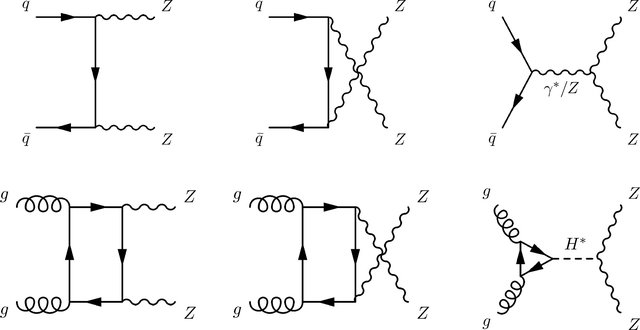
\includegraphics[clip,trim=0.cm 0.cm 15cm 6.5cm, height =2cm]{Figures/c4/dia/Lowest-order-Feynman-diagrams-for-ZZ-production.jpeg}
  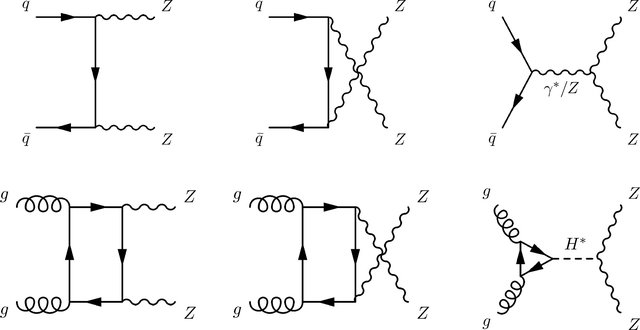
\includegraphics[clip,trim=15.cm 6.cm 0cm 0cm, height =2cm]{Figures/c4/dia/Lowest-order-Feynman-diagrams-for-ZZ-production.jpeg}
  \caption{WZ associated production diagrams (top), ZZ associated
    production diagrams (bottom)~\cite{diagram}.}
  \label{fig:c41}
\end{figure}
The associated production of two \PZ bosons can enter as background in
the three lepton final states when one of the leptons fails
reconstruction or identification requirements. The events present low \ptmiss
values and they have just a few jets and zero b jets. 

\paragraph{W/Z and photon radiation.}\label{sec:c4photon}
In an event, real or virtual photons can appear due to initial state
radiation (ISR) or final state radiation (FSR). In the first case,
partons in the incoming protons emit low energy/collinear radiation
prior to the hard scattering process. For FSR, collinear photons are emitted by
the final states particles.\\
Events (Figure~\ref{fig:c43}) presenting either a W or a Z boson in association with a real or virtual
photon from ISR or FSR can extensively contribute to
the background in three lepton final states.\\
This is the case when a virtual photon decays (internal
conversion) or in which a real photon converts into leptons by interacting with the detector material
(external conversion). The photon can undergo an
asymmetric internal or external conversion in which one of the leptons
has very low $\pt$. This soft lepton has a high probability of failing
the selection criteria of the analysis, leading to a reconstructed
two- (in case of a $\PW$ boson) or three-lepton (in case of a $\PZ$
boson) final state. This background mostly contributes to categories
with an OSSF pair.\\
For the displaced lepton analysis presented in Chapter~\ref{Chapter6}
the external conversion is a ``nasty'' background because it can mimic
a HNL decay vertex where $e^{+}e^{-}$ is produced. In order
to reduce this background either requirements on the kinematic
properties of the event or a material veto can be applied. The latter
helps in rejecting all the SV
which are located in proximity either of a detector layer or of an inert material.

\begin{figure}[h!]
\centering
  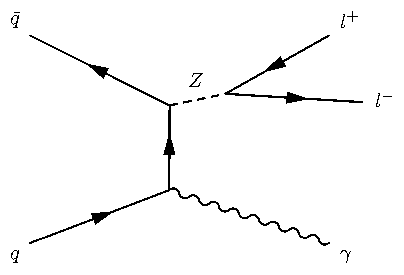
\includegraphics[width=0.23\textwidth]{Figures/c4/dia/40000101.pdf}
  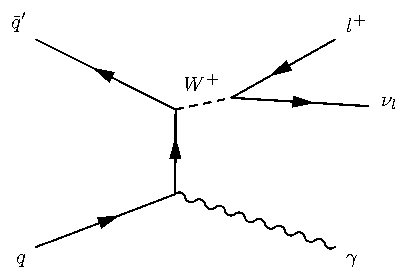
\includegraphics[width=0.23\textwidth]{Figures/c4/dia/40000111.pdf}
  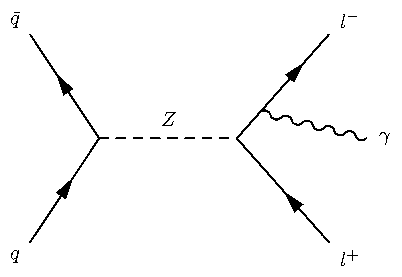
\includegraphics[width=0.23\textwidth]{Figures/c4/dia/40000104.pdf}
  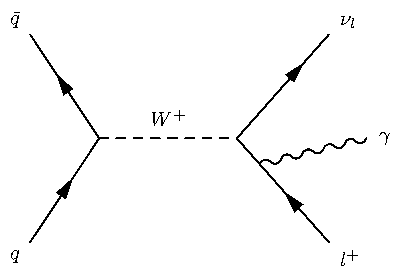
\includegraphics[width=0.23\textwidth]{Figures/c4/dia/40000114.pdf}
  \caption{\PW or \PZ plus $\gamma$ production diagrams. The two
    diagrams on the left represent an initial state
radiation event in association with W/Z production. The two on the
right show an final state
radiation subsequent to W/Z production~\cite{diagram}.}
  \label{fig:c43}
\end{figure}

\paragraph{Drell-Yan production.}\label{sec:c4dy}
The Drell-Yan process happens when a quark from one of the initial
protons annihilates with an anti-quark from the other proton leading to a virtual
photon, $\gamma^{*}$ or to a
\PZ boson, which then decays into two leptons.

\begin{figure}[h!]
\centering
  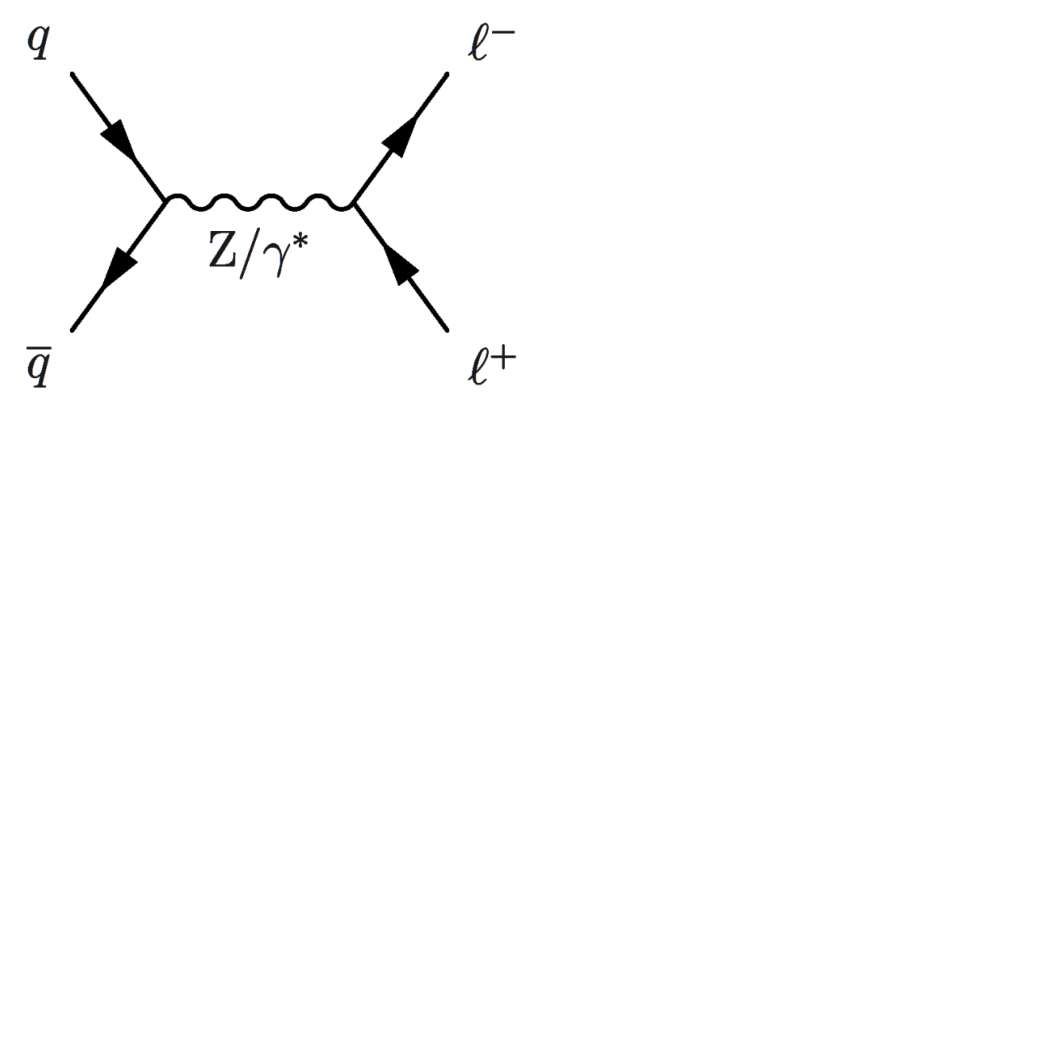
\includegraphics[clip,trim=0cm 10cm 8.8cm 0cm, width=0.25\textwidth]{Figures/c4/dia/dy.pdf}
 \caption{Drell–Yan dilepton production~\cite{diagram}.}
  \label{fig:c44}
\end{figure}
Drell-Yan events contribute in three prompt leptons final states when
associated with a jet production (DY plus jets) or when one nonprompt
lepton is reconstructed and passes the analysis selection. The Drell-Yan
production cross section is so large with respect to other three
leptons processes that even a modest misidentification probability can
lead to a large background contribution.

\begin{figure}[h!]
\centering
 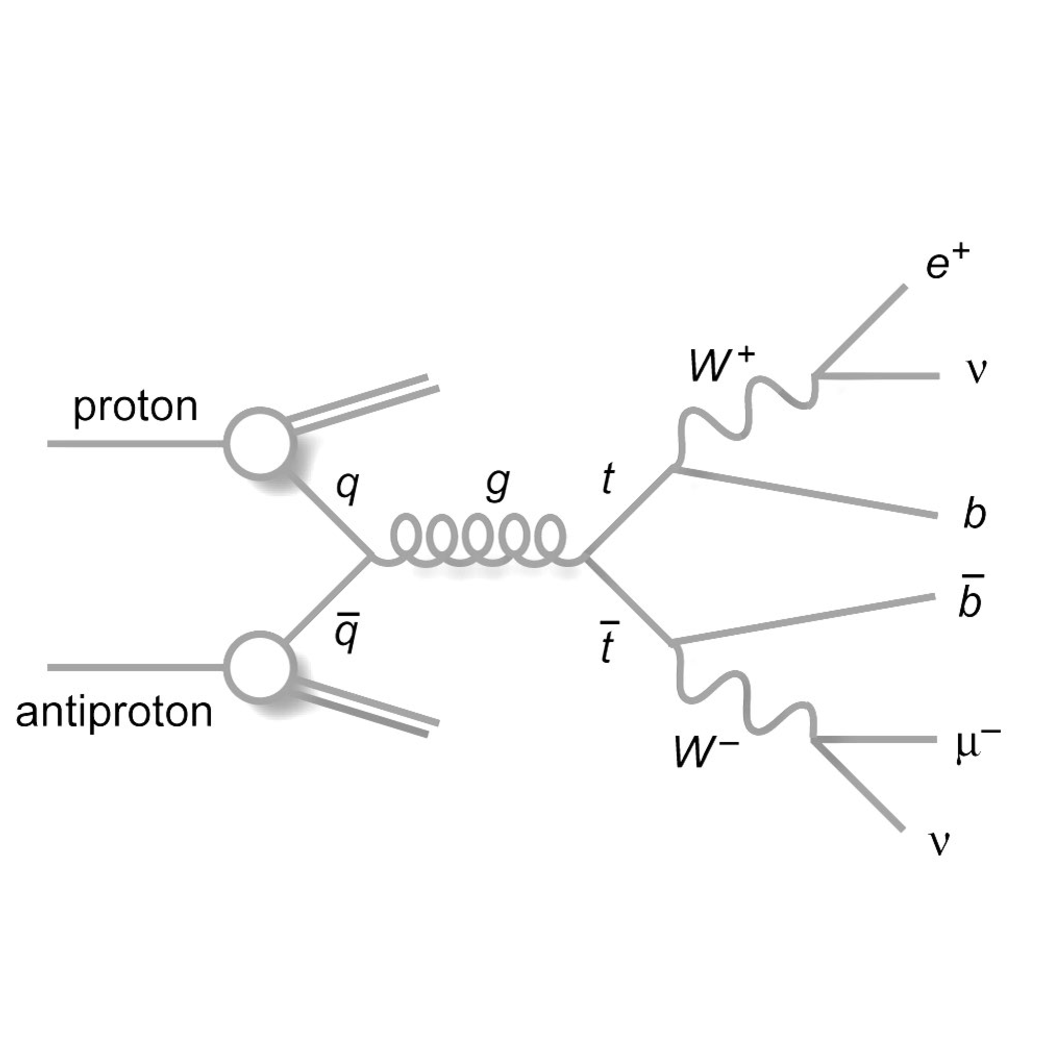
\includegraphics[clip,trim=0cm 3cm 0.2cm 3cm, width=0.45\textwidth]{Figures/c4/dia/tt.pdf}
  \caption{Diagram for $t\bar{t}$ production.~\cite{diagram}}
  \label{fig:c46}
\end{figure}

\paragraph{Top quark production.}\label{sec:c4ttbar}

In both the analysis presented in the following two chapters, the
background from top quark production ($t\bar{t}$) is among the
dominant ones. \\
In this case, the three leptons come from $t\bar{t}$ production 
where they originate from semi-leptonic b quark decay and lepton \PW decay.

\vspace{10mm}
\subsection{Long-lived particles}\label{sec:c4LLbgk}
Long-lived HNL search looks for displaced
vertices and displaced leptons produced relatively far from the PV.
This kind of signature happens to be very different with respect to the
very well known SM processes. Along these lines, the backgrounds
are not the conventional ones and
therefore special care has to be used in understanding them.
\begin{figure}[h!]
\centering
 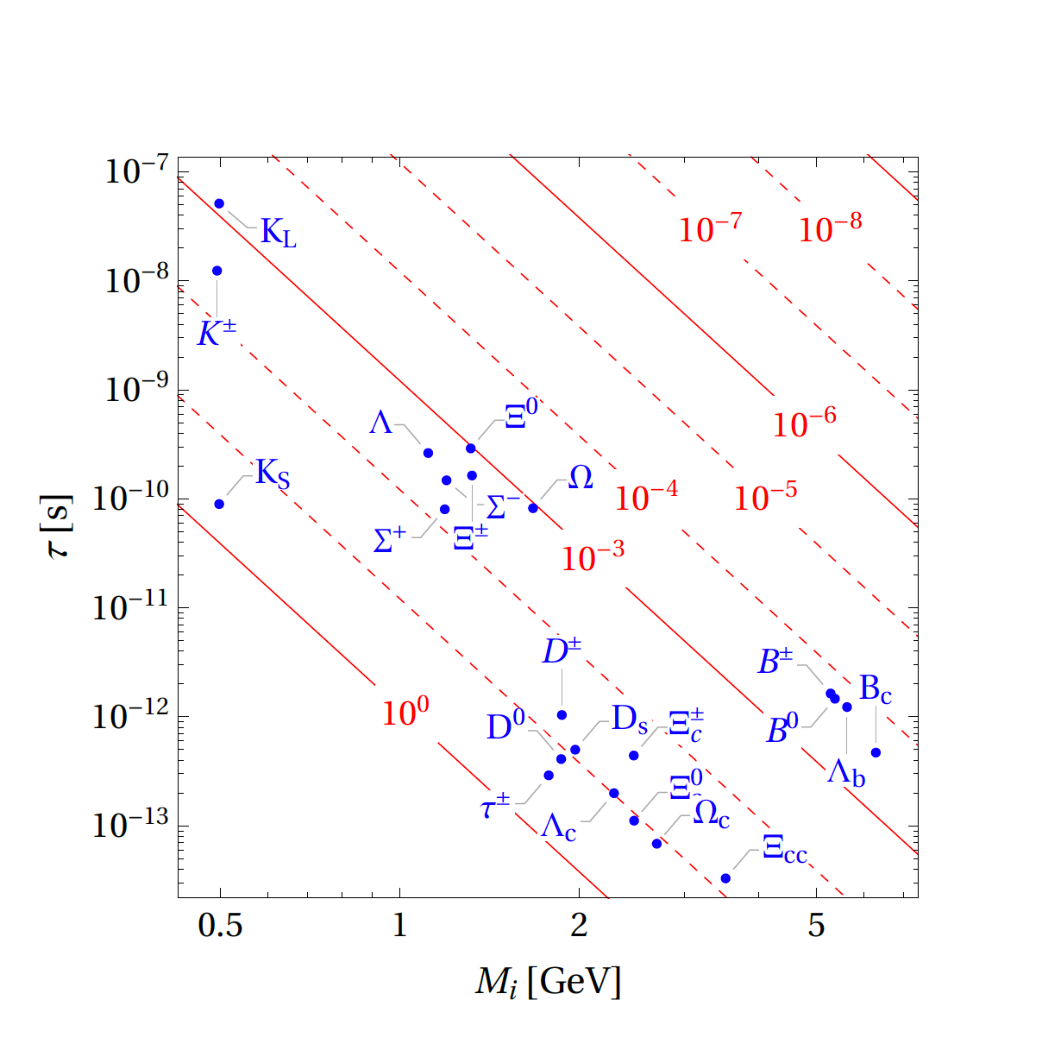
\includegraphics[clip,trim=0.5cm 0.5cm 2cm 2cm, width=0.80\textwidth]{Figures/c4/resonances.pdf}
  \caption{HNL \mixpar (red lines) superimposed with potentially important SM backgrounds
(blue dots) as function of HNL mass and life time~\cite{Drewes_2020_jan}.}
  \label{fig:c4LLbgk}
\end{figure}


In Figure~\ref{fig:c4LLbgk} the phase space of long-lived HNLs is
superimposed with potentially important backgrounds coming from
long-lived meson and baryon decays. The figure shows the crowded area as function
of HNL mass and life time.\\
It is clear from Figure~\ref{fig:c4LLbgk} that the resonance
backgrounds can be rejected with proper criteria according to
the phase space we are investigating.
The top-right corner of Figure~\ref{fig:c4LLbgk} is
background free because it marks a region with very displaced particles
with relative high masses; in this region we will not need to implement
any selection to remove B and D meson contribution. In the central
region of Figure~\ref{fig:c4LLbgk}, $m_\hnl \sim 1$\GeV, we find several
baryons with relative small lifetimes. In this cases, implementing a 
veto on a narrow mass window only for those events with small
displacement could help in rejecting them. The same mass veto is redundant
for events with larger displacement in the same mass region.
This strategy will be presented in
Chapter~\ref{Chapter6} where carefully selected mass windows are removed
to avoid background contamination.




\clearpage
\section{Heavy Neutrino signal event Generation}\label{sec:c4hnl}
This section is strictly relevant to the signal model used in
Chapters~\ref{Chapter5} and~\ref{Chapter6}. The model is circumscribed to the
CMS results only and it is not adopted for ATLAS's
results (~\cite{atlasintro2}) which are often used for comparison
purposes with the CMS results.



\subsection{Signal simulation}\label{sec:c4hnlmodel}

Signal samples are generated using the
\texttt{MadGraph5\_aMC@NLO}~\cite{Alwall_2014} software. 
The generator is used with next-to-leading order (NLO) precision
in perturbative quantum chromodynamics (QCD) for the prompt HNL
model, and at leading-order (LO) precision for the long-lived model.
 %in the strong coupling constant $\alpha_{\mathrm{S}}$.\\
The generation is based on the \texttt{heavyN} model described in
Ref.~\cite{Atre:2009rg}, which is available in Universal FeynRules
Output (UFO) by Ref.~\cite{Alva:2014gxa,Degrande_2016,heavyN}.
This model extends the SM with up to three RH neutrinos,
which are singlets under the SM gauge symmetry.
The mass and mixing parameters of the HNL can be defined for each
scenario to probe.

The HNL production via charged current (CC) Drell-Yan
process,~\ref{fid:hnl_production}(a), via gluon
fusion,~\ref{fid:hnl_production}(b), and via $\PW \gamma$
fusion,~\ref{fid:hnl_production}(c) is simulated. 
\begin{figure}[h!]
\centering
 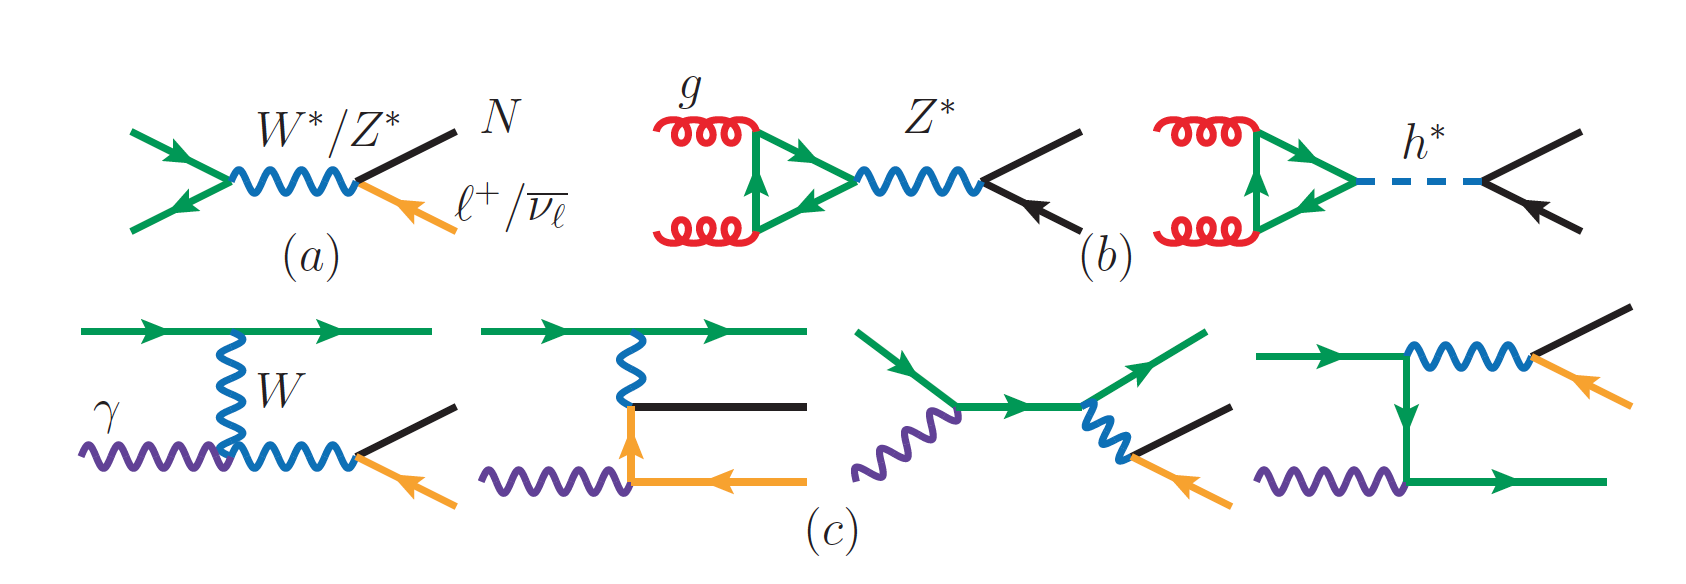
\includegraphics[clip,trim=0cm 0cm 0cm 1cm, width=0.70\textwidth]{Figures/c4/hnl_production}
  \caption{Diagrams for heavy neutrino production mechanisms at
    LHC~\cite{Pascoli_2019}. Each color corresponds to a different
    particle: black = \hnl, yellow = leptons/neutrinos, green =
    quarks, blue = bosons, purble = photons and red = gluons.}
  \label{fid:hnl_production}
\end{figure}

The production mechanisms via gluon and vector-boson fusion are
crucial because
\begin{wrapfigure}{r}{0.48\textwidth}
\centering
  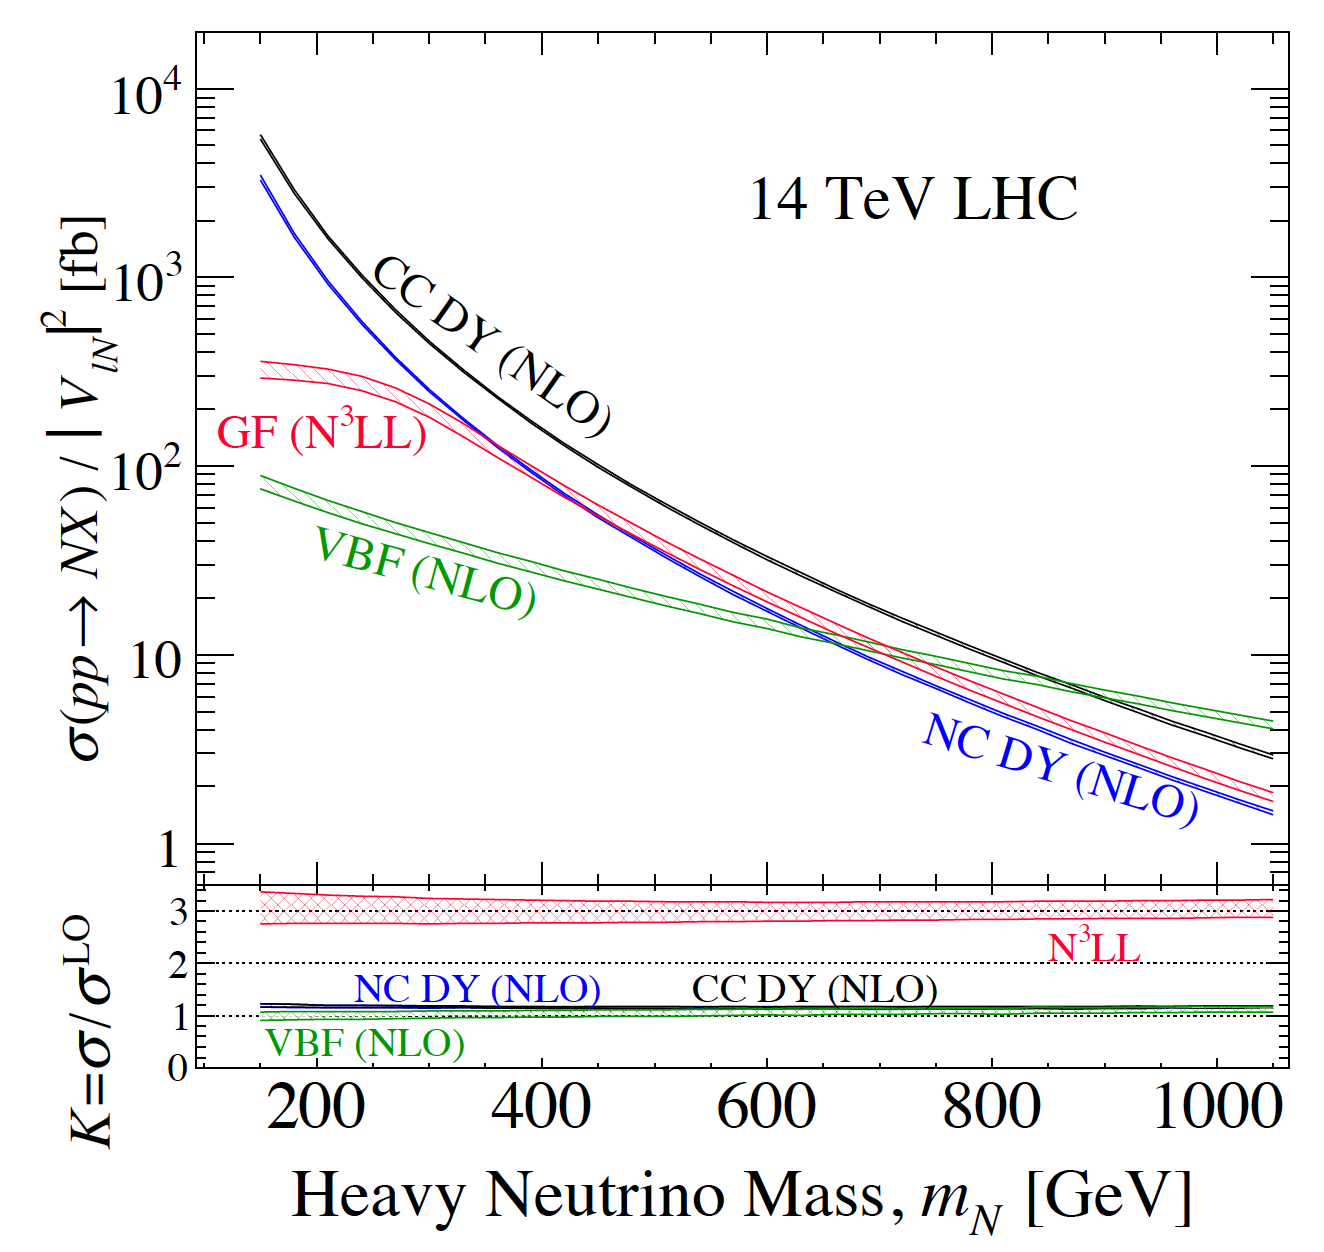
\includegraphics[clip,trim=0cm 0cm 0.5cm 0.5cm, width=.39\textwidth]{Figures/c4/hnl_lhc_production}
  \caption{``HNL production cross section, divided by \mixpar, via
charged (CC) and neutral (NC) current DY, $\PW \gamma$ fusion (VBF),
and gluon fusion (GF) at $\sqrt{s}
\sim 14$\TeV ''~\cite{Pascoli_2019}.}
  \label{fig:hnl_lhc_graph}
\end{wrapfigure} 
 at the LHC energies and at high \hnl mass, the CC DY process
is no longer the only viable way for producing heavy neutrinos. 
Vector boson fusion $\PW \gamma \rightarrow N
\ell^{\pm}$~\cite{PhysRevLett.112.081801, Alva:2014gxa,Degrande_2016}
is the dominant production mechanism at the LHC 
energies for HNLs with very large masses
(TeV energy scale)~\cite{Alva:2014gxa,Degrande_2016, Pascoli_2019} and for
lighter HNLs it enhances the inclusive production rate. Neutral current
processes~\cite{PhysRevD.44.1593,WILLENBROCK1985429}, which involve
gluon fusion, $gg \rightarrow \PZ^{*}/H^{*} \rightarrow \hnl \nu \ell$
can even surpass the CC DY cross section for large HNL masses~\cite{PhysRevD.96.055042,
  Pascoli_2019}. See Figure~\ref{fig:hnl_lhc_graph} for
reference.\\
For the high mass HNL samples used in the search described in
Chapter~\ref{Chapter5}, both gluon
fusion and $\PW \gamma$
fusion are added as production mechanisms. 
The first two employ
the NNPDF3.0 NLO PDFs set~\cite{Ball_2015}, while $\PW \gamma$
fusion uses the LUXqed plus PDF4LHC15 NNLO 100
PDF set~\cite{PhysRevLett.117.242002}.\\
For all the signal MC samples the parton showering and hadronization are simulated with PYTHIA. \\

Samples with HNL masses from 
$\mhnl = 1$\GeV to $\mhnl = 1.2$\TeV are produced for signal
modeling.
The simulated HNLs couple
exclusively to one of the three SM neutrino families at a time with 
mixing probabilities typically in a range $\mixpar = 10^{-6}$ -- 1,
depending on the mass. For this thesis work only the mixing processes between
$\nu_e$--\hnl and $\nu_{\mu}$--\hnl are considered and they are
assumed to be different from zero while the
$\nu_{\tau}$--\hnl is set to zero. The mixing parameters are:
\begin{linenomath}
\begin{equation}
  \mathbf{V}_{\hnl\ell} =
  \begin{pmatrix}
    \mathrm{V}_{\hnl\Pe} & 0 & 0 \\
    0                   & 0 & 0 \\
    0                   & 0 & 0 \\
  \end{pmatrix},
%% \end{equation}
\quad\quad
%% \begin{equation}
  \mathbf{V}_{\hnl\ell} =
  \begin{pmatrix}
    0                    & 0 & 0 \\
    \mathrm{V}_{\hnl\PGm} & 0 & 0 \\
    0                    & 0 & 0 \\
  \end{pmatrix},
%% \end{equation}
\end{equation}
\end{linenomath}
where $\mathbf{V}_{\hnl\ell}$ represents the active-sterile neutrino
mixing matrix:
\begin{linenomath}
\begin{equation}
  \begin{pmatrix}
    \nu_{\Pe}  \\
    \nu_{\PGm} \\
    \nu_{\PGt} \\
  \end{pmatrix} ~=~
  \mathbf{V}_{\hnl\ell}\,\cdot\,
  \begin{pmatrix}
    \hnl_{1} \\
    \hnl_{2} \\
    \hnl_{3} \\
  \end{pmatrix}.
\end{equation}
\end{linenomath}

\begin{figure}[h!]
\centering
 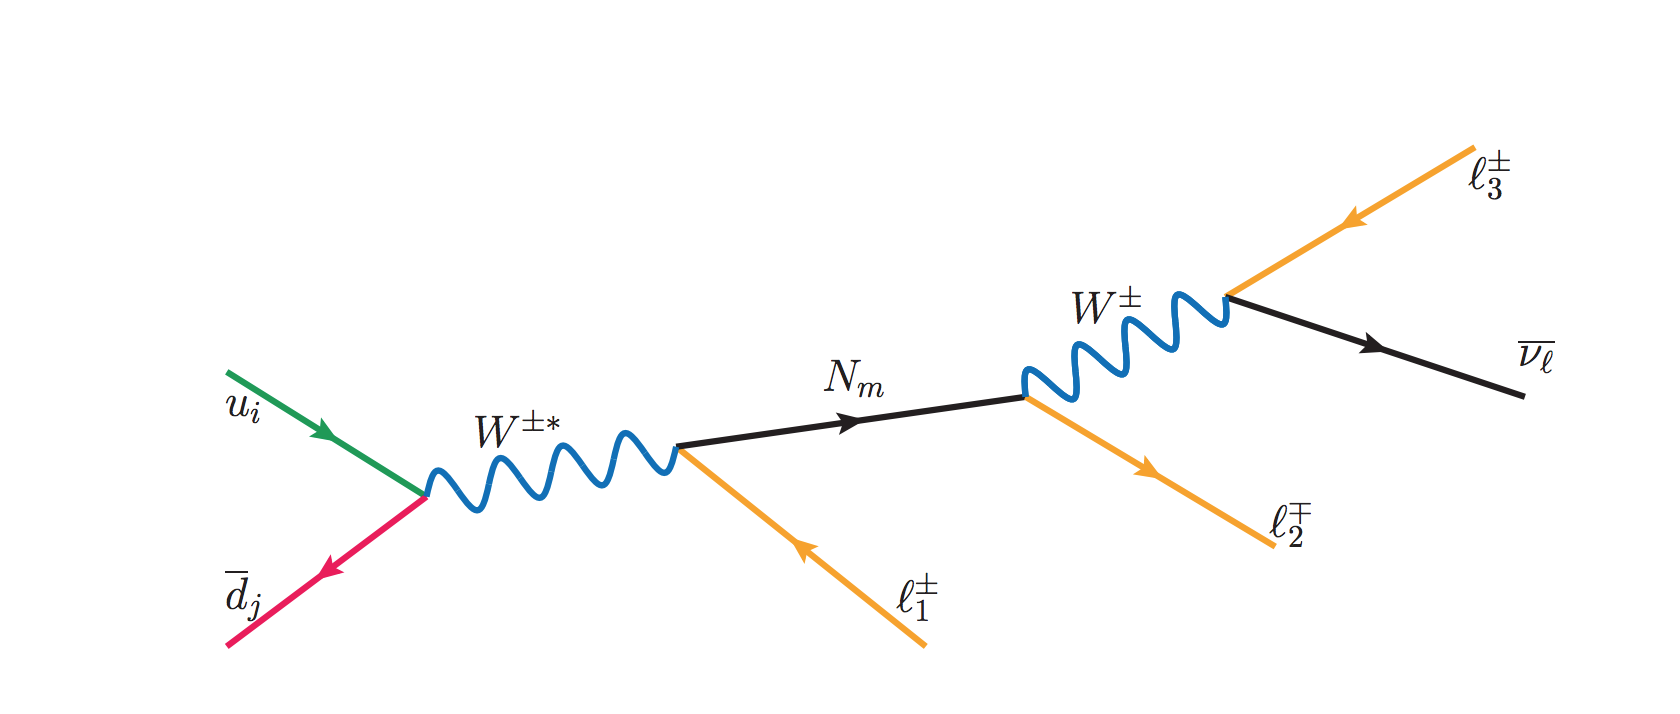
\includegraphics[clip,trim=0.5cm 0.5cm 0.5cm 2.5cm, width=0.75\textwidth]{Figures/c4/hnl_graph}
  \caption{HNL production and decay. Only the leptonic decay of the
    \PW is considered~\cite{Pascoli_2019}.}
  \label{fig:c46}
\end{figure}


\subsubsection{Long-lived HNL samples}\label{sec:reweighting}
For the long-lived HNL, the width $\Gamma_{\hnl}$ is computed automatically by the
generator, and the mean lifetime $\tau_{\hnl} = \hbar/\Gamma_{\hnl}$
is used to extract the HNL lifetime in each simulated event,
according to a decay probability distribution
\begin{linenomath}
  \begin{equation}
\frac{dN(t)}{dt} = \frac{1}{\tau_{\hnl}}e^{-t/\tau_{\hnl}}
  \end{equation}
  \label{eq:dndt}
\end{linenomath}
where $t$ is the
\emph{proper} lifetime, measured in the HNL rest frame.\\
As explained in Section~\ref{sec:promptll}, the values of \mhnl
and \mixpar do not only determine the HNL production cross section,
but also its mean lifetime and, consequently, its kinematics,
acceptance, and reconstruction efficiency.
For a fixed value of \mhnl, therefore, a simple cross section
rescaling is not sufficient to correctly reproduce the behavior of
other HNLs with same mass and different \mixpar.

The simple and naive approach with endless computing power would be an
iterative one. For a \mhnl
and \mixpar scenario, first compute the limits by evaluating parameters
of interest as the overall \emph{signal strength} (number of signal events /
number of expected signal events); when computing the fit between
signal, data and background yields, by default the signal strength is
left floating in the fit, so that the measurement is independent of the
presence or absence of a signal. Depending on the value of the signal
strength there are two options. If the signal strength is below 1 it
means that the \mhnl --\mixpar case is excluded and a new sample with
same \mhnl but smaller \mixpar has to be simulated. If the signal strength is above 1 it
means that the analysis is not sensitive to that \mhnl --\mixpar case and a new sample with
same \mhnl but larger \mixpar has to be simulated. This iteration can
be repeated with steps smaller and smaller until the signal strength is
exactly 1 which means we found the exclusion limits. It is clear that
this kind of approach is not sustainable due to the limited computing
time and available computing power. A smarter correction procedure is needed.\\
To this purpose, a per-event re-weighting technique
based on the HNL lifetime is used instead, which properly accounts for all the
variations in kinematics and acceptance.\\
First, it is noticed that the average kinematics of a HNL decay
is entirely defined by the HNL mass \mhnl, its momentum
$p_\hnl=\beta\gamma\mhnl$, and its decay length,
independently of its mean lifetime $\tau_\hnl$.
Therefore, given a simulated HNL sample of mass \mhnl
and mean lifetime $\tau_0$, we can reproduce the kinematic
distributions of any target HNL scenario with same mass and 
different lifetime, $(\mhnl, \tau_{\mathrm T})$.
An event with proper decay time $t$ taken from the simulated sample
of mean lifetime $\tau_0$ is re-weighted by the ratio of
probabilities to obtain $t$ from $\tau_{\mathrm T}$ or from $\tau_0$:
\begin{linenomath}
  \begin{equation}
    W(t; \tau_0\to\tau_{\mathrm T}) ~=~ \frac{dN_{\mathrm T}(t)/dt}{dN_0(t)/dt} ~=~
    \frac{\tau_0}{\tau_{\mathrm T}}\exp{\left[-t\left(\frac{1}{\tau_{\mathrm T}}-\frac{1}{\tau_0}\right)\right]}.
  \label{eq:ctauReweightingSingle}
  \end{equation}
\end{linenomath}
Taking it a step further, a whole set of multiple HNL samples with different lifetimes
$\{\tau_i\}$ can be used to emulate the $\tau_{\mathrm T}$ scenario. In this case the
decay time distributions must include the correct normalization
factors for each sample, $N_i/\tau_i$, where $N_i$ is the number of
simulated events for the sample with mean lifetime $\tau_i$ and
$N_{\mathrm{tot}} = \sum_i N_i$:
\begin{linenomath}
  \begin{equation*}
    W(t; \{\tau_i\}\to\tau_{\mathrm T}) ~=~ \frac{dN_{\mathrm T}(t)/dt}{\sum_i dN_i(t)/dt} ~=~
    \frac{\frac{N_{\mathrm{tot}}}{\tau_{\mathrm{T}}}\exp{(-t/\tau_{\mathrm{T}})}}
         {\sum_i\frac{N_{i}}{\tau_i}\exp{(-t/\tau_i)}}.
  %\label{eq:ctauReweightingMult}
  \end{equation*}
\end{linenomath}
If $\sigma_{\mathrm{T}}$ is the production cross section for
$(\mhnl,\tau_{\mathrm T})$ and $\mathcal{L}$ is the integrated luminosity,
the complete event weight is
\begin{linenomath}
  \begin{equation}
    w(t; \{\tau_i\}\to\tau_{\mathrm T}) ~=~
    \frac{\sigma_{\mathrm{T}}\mathcal{L}}{N_{\mathrm{tot}}}\,W(t;\{\tau_i\}\to\tau_{\mathrm T})
     ~=~ \frac{\frac{\sigma_{\mathrm{T}}\mathcal{L}}{\tau_{\mathrm{T}}}\exp{(-t/\tau_{\mathrm{T}})}}
         {\sum_i\frac{N_{i}}{\tau_i}\exp{(-t/\tau_i)}}.
  \label{eq:ctauReweighting}
  \end{equation}
\end{linenomath}
Figure~\ref{fig:newReweightGen} compares the proper decay length ($ct$)
distributions for three samples of $\mhnl=4$\GeV with different mean
lifetimes, and the corresponding models built from the sum of the
three samples by re-weighting with Eq.~\ref{eq:ctauReweighting}. An
excellent agreement is observed, with the re-weighted summed sample
exhibiting less statistical fluctuations than the individual samples.
\begin{figure}[h!]
  \centering
  \includegraphics[width = .5\textwidth]{Figures/c4/reweighting/ctau_genLevel_unskimmed.png}
  \caption{Distribution of the proper decay length $ct$ for three HNL
    samples of $\mhnl=4\GeV$ and different mean lifetimes (points withs
    error bars),
    and the corresponding models built from the sum of the three
    samples by re-weighting with Eq.~\ref{eq:ctauReweighting}
    (continuous histograms). The black, continuous histogram shows the
    sum of the three samples, while the black, dashed line is the sum
    of the three exponential functions that describe the proper decay
    length of the three samples. \dani}
  \label{fig:newReweightGen}
\end{figure}
\begin{figure}[h!]
  \centering
  \includegraphics[width = .32\textwidth]{Figures/c4/reweighting/reweighting_mass_M4p0_V0p00251197_mu_18.pdf}
  \includegraphics[width = .32\textwidth]{Figures/c4/reweighting/reweighting_disp_M4p0_V0p00251197_mu_18.pdf}
  \includegraphics[width = .32\textwidth]{Figures/c4/reweighting/reweighting_M4p0_V0p00251197_mu_18.pdf}
  \caption{Distributions of the reconstructed dilepton mass \mtwol
    (left), secondary-vertex transverse displacement \Deltwod (middle), and final signal-region yields described in
    Section~\ref{sec:llbaselinesel} (right), for a HNL scenario with
    $\mhnl=4\GeV$ and $\mixparm = 6.31\cdot 10^{-6}$ in the 2018
    simulation. The black histograms are modeled
    using a single sample with the re-weighting of
    Eq.~\ref{eq:ctauReweightingSingle}, while the red histograms use
    the sum of three samples with different $\mixparm$ values and the
    re-weighting of Eq.~\ref{eq:ctauReweighting}. \dani}
  \label{fig:newReweightRec}
\end{figure}
Figure~\ref{fig:newReweightRec} shows distributions of the
reconstructed dilepton mass (\mtwol) and secondary-vertex transverse
displacement (\Deltwod (~\ref{sec:c2IP})) for a HNL scenario with
$\mhnl=4$\GeV and $\mixparm = 6.31\cdot 10^{-6}$ in 2018,
modeled using either a single sample with the re-weighting of
Eq.~\ref{eq:ctauReweightingSingle} (black histograms), or the sum of
three samples with different $\mixparm$ values and the re-weighting of
Eq.~\ref{eq:ctauReweighting} (red histograms). The two models are compatible.\\
The histograms
presented in Figure~\ref{fig:newReweightRec} are filled with events
that pass the event selection specifically designed for the
long-lived HNL analysis presented in Chapter~\ref{Chapter6}, for details
refer to Section~\ref{sec:llanalisi}. \\

Figure~\ref{fig:hnlSamples} shows the total number of HNL signal
events available for each $(\mhnl,\mixparm)$ point, which were
generated specifically for the long-live HNL search. For each HNL
mass, all the samples produced with different lifetimes
$\{\tau_i\}$ have been used to emulate the $\tau_{\mathrm T}$ scenario.


\begin{figure}[h!]
  \centering
  \includegraphics[clip,trim=0.7cm 0cm 0cm 0cm ,width=1\textwidth]{Figures/c4/mu.pdf}
  \caption{Total number of signal MC events available for each
    $(\mhnl,\mixparm)$ point, considering both private and central CMS
    productions. The number of events can be read with color code
    using the palette on the right; the range is from 100 to 1000 events. The picture can be mirrored for $(\mhnl,\mixpare)$ scenario.}
  \label{fig:hnlSamples}
\end{figure}



\subsubsection{Dirac HNL signal emulation}\label{sec:c4diracmajo}
The HNL production cross section is fixed by the \mhnl and \mixpar
values~\cite{Degrande_2016,heavyN}, and it is the same for Dirac and
Majorana HNLs.
The resonance width for a Majorana HNL, on the other hand, is exactly
twice the width of a Dirac HNL with same \mhnl--\mixpar values, due to
the additional charge-conjugated (LNV) decay channels (refer to Figure~\ref{fig:dirac_majo}).
As a consequence, the average lifetime of a Dirac HNL is twice that of
a Majorana HNL with same $(\mhnl,\mixpar)$. Refer
to Section~\ref{sec:c3majo_dirac}.
\begin{figure}[h!]
\centering
 \includegraphics[clip,trim=0cm 7cm 0cm 3cm, width=0.65\textwidth]{Figures/c4/dirac_majo2}
  \caption{Visualization of the LNV and LVC cases. HNL with a Majorana
    nature contributes to both diagrams, while Dirac type HNL can only
    lead to right side diagram. These diagrams show the specific case
    when \hnl mixes with $\nu_\mu$ only resulting in having $\mu_{1}$
    and $\mu_{2}$. The same diagrams can be made for $e_{1}$
    and $e_{2}$ as well.}
  \label{fig:dirac_majo}
\end{figure}

For the HNL analysis with three prompt leptons (Chapter~\ref{Chapter5}) there is no 
need to produce distinct Dirac and Majorana MC samples since there is
no difference between them except the final state combinations. For the
long-lived scenario separate samples are necessary.

After the lessons learned with the emulation procedure described 
above, a similar idea and strategy
was also adopted for obtaining HNL signal sample for the scenario where HNL has a Dirac nature using the sample where HNL is a Majorana particle.\\
To optimize computing resources and in the interest of time,
high-statistics MC samples were produced on a large scale for Majorana
HNL scenarios only.
Dirac HNL scenarios for any $(\mhnl,\mixpar)$ point were emulated
starting from the corresponding Majorana HNL samples, following these
steps:
\begin{itemize}
\setlength\itemsep{-0.2em}
\item from a Majorana HNL sample, select only the LNC events by
  looking at the unique identity number of the generated particles;
\item re-weight each LNC event to emulate the correct lifetime of the
  Dirac HNL, by using Eq.~\ref{eq:ctauReweightingSingle} with
  $\tau_{\mathrm{T}}=2\tau_0$;
\item since only half the events of the original Majorana sample are
  used (while the cross section is the same for Majorana and Dirac
  scenarios), add a factor 2 to the event weight to restore the correct
  normalization.
\end{itemize}
This method provides a good modeling of the Dirac HNL signal, but
uses only half the events from the Majorana HNL MC samples. With a
simple extra assumption, it is possible to make use of the full
statistical power of our MC production.\\
As explained in Section~\ref{sec:llresults}, the signal selection is the
same for LNC and LNV events. Just in the final stage of the analysis,
events are split into same-lepton-charge and opposite-lepton-charge
categories to distinguish LNV and LNC events for the physics
interpretation. If we assume that the lepton efficiency and
acceptance are the same for positively and negatively charged leptons
(\ie, same reconstruction and identification efficiency, same momentum
scale and resolution, etc.), then we can use both LNC and LNV events
from the Majorana HNL samples to emulate the Dirac scenarios, and
simply classify all of them as opposite-charge events. In fact, any
difference in the performance of positive and negative leptons is
expected to be negligible, certainly well below the systematic
uncertainties assigned to the displaced leptons (see
Section~\ref{sec:displeptoneff}).
This approach allows us to use all the available events from the
Majorana HNL samples in the Dirac HNL interpretation.\\
Figure~\ref{fig:majToDirReweighting} shows a comparison between Dirac
HNL samples and Majorana HNL samples corrected to emulate Dirac
scenarios, employing both strategies outlined above.
As can be seen, differences are small accros the most relevant observables  for defining the search strategy.
\begin{figure}[h!]
  \centering
  \includegraphics[width = .32\textwidth]{Figures/c4/reweighting/diracReweighting_M-2_V-0p0157162336455_mu_mass_18.pdf}
  \includegraphics[width = .32\textwidth]{Figures/c4/reweighting/diracReweighting_M-2_V-0p0157162336455_mu_disp_18.pdf}
  \includegraphics[width = .32\textwidth]{Figures/c4/reweighting/diracReweighting_M-2_V-0p0157162336455_mu_18.pdf}
  \caption{Distributions of the reconstructed dilepton mass \mtwol
    (left), of the transverse displacement of the reconstructed
    HNL decay vertex \Deltwod (middle), and event yields in the
    different analysis categories (right) for a Dirac HNL with
    $\mhnl=2$\GeV and $\mixparm=2.47\times 10^{-4}$ in 2018
    simulation, using three models: a Dirac HNL sample (black), or a
    set of Majorana HNL samples with $\mhnl=2$\GeV and various
    $\mixparm$ values, re-weighted to emulate the Dirac scenario with
    $\mixparm=2.47\times 10^{-4}$, using LNC events only (blue) or all
    events (red). \dani} 
  \label{fig:majToDirReweighting}
\end{figure}


\subsubsection{Uncertainty on LL-signal MC cross section}\label{sec:c4lo}
The \texttt{heavyN} model used for generation of long-lived HNL events does not allow for NLO QCD calculations. The simulation of HNL events happens therefore at LO, resulting in large theoretical uncertainties on the cross section (up to $15\%$) that have to cover the effect of the missing higher order QCD corrections and PDF uncertainties.

Instead of relying on these LO uncertainties, a general correction factor for the cross section from LO to NNLO can be derived based on the SM production of \PW\ $\rightarrow$ $\ell$ $\bar{\nu}$ . In HNL production, the only difference from this SM process is the exchange of the SM neutrino by a HNL. The effect of the mass and coupling of the HNL can be factorized in the calculation of the HNL cross section and is not affected by the PDF and scale variations. The dominant effect of these uncertainties appears at the production of the \PW boson, therefore it can be studied in the SM process \PW\ $\rightarrow$ $\ell$ $\bar{\nu}$ , for which recommended values for the cross section at NNLO exist with their corresponding theory uncertainties. Our approach is to get a LO cross section for \PW\ $\rightarrow$ $\ell$ $\bar{\nu}$ calculated with Madgraph using the same exact conditions as the HNL MC production. A correction factor from LO to NNLO can be derived based on this and can then be applied to HNL MC. The PDF and scale uncertainties at NNLO are applied as flat systematic uncertainties to cover the remaining uncertainty on the MC cross section.

It has been checked and verified that the generator conditions are similar between our MC production and the centrally produced W+jets samples, from which the recommended NNLO cross section was taken. The small differences that are present have no significant effect on the cross section calculation. Additionally, lepton universality will allow us to apply the scale factor and uncertainty across all HNL samples, regardless of which lepton flavor(s) they couple with.

The resulting LO cross section for \PW\ $\rightarrow$ $\ell$
$\bar{\nu}$ ($\ell$ = \Pe\ , \PGm\ , \PGt\ ) is 56500 pb. The recommended NNLO value is $61526.7^{+497.1}_{-264.6}\pm 2312.7$ pb where the quoted uncertainties are respectively scale and PDF uncertainties. Assuming uncorrelated uncertainties and taking the maximum of the two asymmetric errors, the combined uncertainty is $61526.7 \pm 2365.5$ pb, an effect of $3.86\%$. This gives a final scale factor of $1.089 \pm 0.042$.

\section{Data sets}\label{sec:c4data}

For each CMS analysis according to the final states we 
select, a specific type of primary datasets (PDs) is used.\\
The definition of the primary datasets is intrinsically connected to
the HLT trigger paths (~\ref{sec:triggersystem}). The PD design is centered
around particles reconstructed in the event by the HLT, and follows one simple principle:
grouping together events with similar physics content; for instance, there are
single-lepton datasets and double-leptons datasets.
Since an event can pass more than one HLT path,
it can enter in more than one primary dataset. At a practical level, possible overlaps among different datasets are
removed by checking run, lumi-section, and event numbers in order to not have twice the same event coming from different PDs.\\


The analysis presented in Chapter~\ref{Chapter5} includes
\texttt{SingleElectron}, \texttt{SingleMuon}, \texttt{DoubleEG},
\texttt{DoubleMuon} and \texttt{MuonEG} primary datasets; the choice was driven by the
multiple trigger requests, both single lepton trigger and
dilepton triggers in order to maximize the trigger efficiency.

The analysis presented in Chapter~\ref{Chapter6} includes only
\texttt{SingleElectron} and \texttt{SingleMuon} for signal search,
while \texttt{DoubleEG} and
\texttt{DoubleMuon} primary datasets are used for background
measurements. For this specific case the choice was
made considering the limitations due to the presence of displaced
leptons in the final states.
Since (most of) the CMS leptonic triggers are
optimized for prompt lepton identification, it was decided
to use single-electron and single-muon triggers for the
signal selection.\\

The first analysis presented in the following chapters used only 
\Pp collision data collected
by the CMS experiment at center-of-mass energy of 13\TeV
in 2016, corresponding to an integrated luminosity of 35.92\fbinv.\\

The long-lived HNL analysis uses three sets of \Pp collision data
corresponding to three years of data-taking at a
center-of-mass energy of 13\TeV, corresponding to integrated
luminosities of 35.92\fbinv (2016), 41.53\fbinv (2017), and 59.97\fbinv
(2018). 

\section{Summary}\label{sec:summaryC4}
In this chapter an overview of the simulated signal and main background samples and the data sets
samples is presented.\\
We first introduced the different ``ingredients'' that compose the
background of the analyses presented in Chapters~\ref{Chapter5}
and~\ref{Chapter6}. We tried to explain which SM processes can
contribute and contaminate the signal region accidentally passing the object and event selection criteria. Taking into account the three prompt
leptons final state scenario, we listed the processes that better
mimic the signal signatures while having a sizable branching
ratio and large production cross-sections. 

We described the HNL model adopted in the context of this thesis. The
main features were presented with a large focus on
long-lived HNL case. In this framework the re-weighting procedure was
introduced, which is going to be a key point for the 
interpretation of the results in both the prompt and displaced heavy neutral lepton
analyses of Chapters~\ref{Chapter5}
and~\ref{Chapter6}.

Finally details about data taking, data campaigns and primary datasets were presented.


 
\chapter{Search for HNL in events with three charged prompt
  leptons} \label{Chapter5}

The first search~\cite{Sirunyan:2018mtv} on HNLs using a multilepton
final state at the CMS
experiment is presented here. The targeted signature comprises 
three prompt charged leptons in any flavor combination of electrons
and muons. 

\section{Introduction}
The search probes direct heavy neutrino production in the decay of W
bosons, in which the SM neutrino oscillates into a HNL. The focus
lies on events in which the HNL decays either into a Z boson and a
neutrino, or into a W boson and a charged lepton. The resulting
electroweak gauge boson can then decay leptonically, leading to a
final state with three charged leptons and a neutrino. The Feynman diagrams corresponding to the described processes are shown in 
Figure~\ref{fig:c5hnldiagram}. Further, a Majorana HNL can decay
furthermore into a lepton with either same-sign (Figure~\ref{fig:c5hnldiagram} left) 
or opposite-sign (Figure~\ref{fig:c5hnldiagram} right) with respect to the lepton, $\ell$, coming directly from \PW boson. 
\begin{figure}[h]
\centering
\includegraphics[width=0.4\textwidth]{Figures/c5/hnl_feyn.pdf}
\includegraphics[width=0.4\textwidth]{Figures/c5/hnl_feyn_2.pdf}\\
\includegraphics[width=0.4\textwidth]{Figures/c5/hnl_z_feyn.pdf}
\includegraphics[width=0.4\textwidth]{Figures/c5/hnl_z_feyn_2.pdf}
\caption{Typical diagrams for the production of a HNL ($\hnl$)  at the LHC \ti
through its mixing with a SM neutrino, leading to a
final state with three charged leptons and a neutrino.}
\label{fig:c5hnldiagram}
\end{figure}

The final results of this analysis will be presented as sensitivity
curve as a function of both the mass and the mixing parameter, \mixpar
of the HNLs. 

\section{Analysis setup}
\subsection{Data and simulation samples}
The current analysis uses the set of \Pp collision data collected during the 2016 run at center-of-mass energy of 13\TeV corresponding to
an integrated luminosity of 35.9 \fbinv. 

A number of signal models, as described in the previous
Chapter, Section~\ref{sec:c4hnlmodel}, were simulated with NLO precision in
perturbative QCD. 

The luminosity scenario has a 25~ns bunch crossing separation with an
average of about 23 pileup interactions per bunch
crossing, for details refer to Section~\ref{lhc}.

\subsection{Signal compression and trigger strategy}\label{sec:compression}
A challenging aspect of the signal under consideration is that, except
for very high masses, the \pt
spectra of the resulting leptons are in general very soft and they are
all collected in the same low \pt region; we can say that the \pt
spectra are compressed. The degree of this compression, and which
leptons are affected, depends on the mass of the produced HNL. The \pt
spectrum of the three highest \pt generator-level charged leptons is shown in figure~\ref{fig:genPt} for different HNL mass scenarios, ranging from 5 to 200 \GeV . 

\begin{figure}[h]
\noindent
\makebox[\textwidth]{
\subfloat[]{\includegraphics[width=.3\textwidth]{Figures/c5/genPt/genPtm5.pdf}}
\subfloat[]{\includegraphics[width=.3\textwidth]{Figures/c5/genPt/genPtm60.pdf}}
\subfloat[]{\includegraphics[width=.3\textwidth]{Figures/c5/genPt/genPtm200.pdf}}}
\caption{\pt spectrum of the three highest generator-level leptons in
  the signal simulation of several HNL masses. From top left to bottom
  right the HNL mass scenarios for which the spectrum is shown are
  5\GeV (A), 60\GeV (B), and 200\GeV (C). \willem}
\label{fig:genPt}
\end{figure}

It can be seen that for every mass scenario below the W-mass, one or
more leptons have a tendency to have very low \pt values. For low mass
samples both the trailing and sub-leading leptons are soft because of
the small mass of the decaying HNL. For HNL masses close to the mass of
the W, very little phase space is left for the emission of the lepton
in the W's decay since all of the W's mass has to go into the
production of the HNL. For high masses on the other hand, the
compression is not as pronounced even though the trailing lepton can
still be seen to prefer relatively low momenta because of the high off-shell W-boson required for production of very heavy
HNL's. Furthermore the cross section for off-shell W-boson production drops
rapidly with increasing mass, and as such the lepton with smallest \pt
also tends to have very little phase space available for its production in
very high mass scenarios.

We can clearly notice in Figure~\ref{fig:genPt} different lepton \pt spectra according to the
$M_\hnl$ and the correlation between the distributions and the $M_\PW$. For this reason the analysis
strategy has been divided in two main phase spaces:
\begin{itemize}
\setlength\itemsep{-0.2em}
\item \emph{low mass search:} soft leptons, $M_\hnl < M_\PW$;
\item \emph{high mass search:} hard leptons, $M_\hnl > M_\PW$;
\end{itemize}

\subsubsection{Trigger strategy}
Due to the low \pt spectra of the leptons in the HNL signals, designing a trigger strategy is a challenging task. 
For high HNL masses, the leading lepton \pt is generally on the efficiency plateau of the single-lepton triggers.
For low HNL masses, we need to add double- and triple-lepton triggers to obtain optimal signal efficiency.
The list of triggers used in this analysis are listed in table~\ref{table:HNL_trigger_thresholds}.


\begin{table}[h]
\centering
{\scriptsize
 \caption{Overview of the lepton \pt thresholds imposed in the analysis and the \pt regime in which each trigger path provides sensitivity.}
  \label{table:HNL_trigger_thresholds}
  \begin{tabular}{c|c|ccc|l}
   \hline
    search region                  & lepton flavors                    & \multicolumn{3}{c|}{selected \pt range (\GeV)} & sensitive trigger paths \\
                                   & $\ell^{\text{leading}} \; \ell^{\text{subleading}} \; \ell^{\text{trailing}}$ & $\pt^\text{leading}$ & $\pt^\text{subleading}$ & $\pt^\text{trailing}$ & \\
    \hline
    \multirow{12}{*}{low mass}     & $ee\mu$                           & 30--55 & $>15$    & $>5$     & $1e$ \\
                                   &                                   & 15--30 & $>15$    & $>8$     & $2e1\mu$ \\
                                   &                                   & 23--30 & 10--15    & $>8$     & $1e1\mu$ \\
                                   &                                   & 25--30 & $>15$    & 5--8      & $2e$ \\
                                   & $e\mu e$, $\mu ee$                 & 30--55 & $>15$    & $>10$    & $1e$ or $1\mu$ \\
                                   &                                   & 15--30 & $>15$    & $>15$    & $2e1\mu$ \\
                                   &                                   & 23--30 & $>10$    & 10--15    & $1e1\mu$ \\
                                   & $\mu\mu e$                        & 30--55 & $>15$    & $>10$    & $1\mu$ \\
                                   &                                   & 15--30 & $>10$    & $>10$    & $1e2\mu$ \\
                                   & $\mu e \mu$, $e\mu\mu$            & 30--55 & $>10$    & $>10$    & $1e$ or $1\mu$ \\
                                   &                                   & 15--30 & $>10$    & $>9$     & $1e2\mu$ \\
                                   &                                   & 23--30 & $>10$    & 5--9      & $1e1\mu$ \\
    \hline
    high mass                      & all flavors
                                                                       & $> 55$    & $>15$    & $>10$  & all paths \\
 \hline
  \end{tabular}
}
\end{table}

The overall approach to selecting the offline thresholds in the analysis is the following:
.


\begin{itemize}
\setlength\itemsep{-0.1em}
\item Each trigger path could select one or more leptons (refer to
  table~\ref{table:HNL_trigger_thresholds} for all the used trigger paths); furthermore for
  each lepton a specific efficiency can be individually measured, it
  will be referred as lepton-specific efficiency. Then data/MC scale
  factors (SF) are calculated for each used
  lepton-specific trigger and determine values where these SFs are
  constant. 
 Typical SF values are 98\% for a muon-specific and 99\% for an electron-specific. 
\item determine total efficiency of trigger combinations (not anymore
  lepton-specific) in MC simulation, and choose \pt thresholds leading to the high overall efficiency and being not lower than the values determined in the first step;
\item check the overall data/MC SF in an orthogonal and unbiased dataset which was
  selected by triggering on \ptmiss or the hadronic activity of the event;
\item determine systematics from the SF values obtained in the first step and validate its choice in the previous step: 
\begin{itemize}
\item use 5\% systematics for events with leading lepton $\pt < 30$\GeV (max. SF value for $\Pe\Pe\mu$ and $\Pe\mu\mu$ case),
\item and 2\% for events with leading lepton $\pt > 30$\GeV (max. SF value of a muon leg).
\end{itemize}
\item require trigger information in MC samples when deriving the yields, but not apply any additional correction.
\end{itemize}


\iffalse
We use the tag-and-probe method to measure the lepton-specific efficiencies. The efficiency is 
defined as the ratio of selected events where the probe matches the lepton-specific in question ($\Delta R<0.4$) over 
the total number of selected events. Events entering the denominator in data are taken from the 
SingleElectron (SingleMuon) dataset and must fire an unprescaled
single lepton trigger with \pt threshold > 27\GeV (> 24\GeV).
Requiring the tag and the probe to both pass the offline lepton selection reduces the contamination 
from fakes at sub-percent level. We therefore do not perform any background subtraction using a fit to 
the \PZ peak. This choice presents the advantage that the measurement in channels purely dominated by the 
Drell-Yan process ($\Pe\Pe$ and $\mu\mu$) can be compared to a channel where the contribution from \ttbar 
becomes dominant at high lepton $\pt$ ($\Pe\mu$).
In order to estimate the uncertainty on the trigger efficiency for the OR combination of single, double and trilepton triggers,
we select trilepton events according to the baseline selection criteria described in Section~\ref{sec:object}.
The trigger efficiency is then measured as a function of the trailing
lepton \pt in both the unbiased \verb!MET! dataset, a high-statistics $\PW\PZ$ MC sample and a HNL samples. 
The applied baseline selection criteria
ensures we are on the efficiency plateau, see Figure~\ref{fig:3l1l1lEff}, and reasonable data/MC agreement is observed 
as statistical uncertainties of the samples allow to judge.}
\fi

The overall $1\ell+2\ell+3\ell$ trigger efficiency was measured in WZ MC samples 
after selecting 3 leptons with relevant flavor combination which pass
the offline analysis ID. The efficiency is typically close to 100\%
and always above 92\%, for events with leading lepton \pt $> 30$\GeV. For
events in which the leading lepton \pt is $< 30$\GeV, the efficiency
falls down reaching the value of 70\% in the worst case scenario.
Hence we assign a 5\% uncertainty
on the trigger efficiency for leading lepton $\pt < 30$\GeV
$\;$ and for $\pt > 30$\GeV we assigned a 2\%
uncertainty. 

\iffalse
\begin{figure}[h]
\noindent
\makebox[\textwidth]{
  \subfloat[{\tiny$3\Pe$, $\pt^\text{lead} > 55\GeV$}]{\includegraphics[width=0.34\textwidth]{Figures/c5/trigger/vsTrailingPt/eee_pt55to1000.pdf}}
  \subfloat[{\tiny$3\mu$, $\pt^\text{lead} > 55\GeV$}]{\includegraphics[width=0.34\textwidth]{Figures/c5/trigger/vsTrailingPt/mumumu_pt55to1000.pdf}} 
  \subfloat[{\tiny$2\Pe1\mu$, $\pt^\text{lead} [15,30] $}]{\includegraphics[width=0.34\textwidth]{Figures/c5/trigger/vsTrailingPt/eemu_pt0to30.pdf}}}\\
  \noindent
\makebox[\textwidth]{
  \subfloat[{\tiny$2\Pe1\mu$, $\pt^\text{lead} [30,55] $}]{\includegraphics[width=0.34\textwidth]{Figures/c5/trigger/vsTrailingPt/eemu_pt30to55.pdf}} 
  \subfloat[{\tiny$1\Pe2\mu$, $\pt^\text{lead} [15,30] $}]{\includegraphics[width=0.34\textwidth]{Figures/c5/trigger/vsTrailingPt/emumu_pt0to30.pdf}}
  \subfloat[{\tiny$1\Pe2\mu$, $\pt^\text{lead} [30,55] $}]{\includegraphics[width=0.34\textwidth]{Figures/c5/trigger/vsTrailingPt/emumu_pt30to55.pdf}}}\\
  \caption{Efficiencies for the OR combination of single, double and trilepton triggers, in trilepton events as a function
  of the trailing lepton \pt.}
  \label{fig:3l1l1lEff}
\end{figure}
\fi

\subsection{Object selection}\label{sec:object}
For the rigorous explanation of the single object reconstruction in
CMS see Chapter~\ref{Chapter2_5}, section~\ref{sec:reconstruction}.

\subsubsection{Leptons}
The base objects of this analysis are electrons and muons. Both
electrons and muons have three selection working points, called
\textsc{loose}, \textsc{fakeable object} (\textsc{FO}) and \textsc{tight}~\footnote{
N.B. these working points do not necessarily coincide with the ones
defined in Sections~\ref{sec:c2muonselection}
and~\ref{sec:c2keleid}. For these latter the italic style is used.} which
are specifically delineated for this analysis. The \lo working point
is used when cleaning electrons from overlap with muons, to be
specific, electrons are not considered for selection if they fall
within a cone of $\Delta \mathrm{R} = 0.05$ around a \lo muon. The
\fo working point is slightly tighter than the \lo one, and is
extensively used for the estimation of the background due to
non-prompt and fake leptons as described further in this text. The
ideal feature of a typical \fo working point is that after applying it
the probability that a selected non-prompt lepton also passes the
\ti working point should be independent
 of the flavor of its origin parton.
 This property will prove essential for the non-prompt lepton background estimation as further specified. The full definitions of every selection working point, for respectively muons and electrons are shown in tables ~\ref{tab:muonIDs} and \ref{tab:eleIDs}.

Signal leptons are required to be isolated (refer to
Section~\ref{sec:c2iso}) from any hadronic activity
in the event. \lo and \fo leptons are required to have $\Irel < 0.6$. 
\ti leptons must satisfy $\Irel < 0.1$.

\begin{table}[h!]
\centering
{\scriptsize
\caption{All the variables used in the table are introduced in
  Chapter~\ref{Chapter2_5} in Sections~\ref{sec:reconstruction},~\ref{sec:c2muonselection}
 and~\ref{sec:c2variables}.
Requirements to pass each definition of the muon selection.}
\label{tab:muonIDs}
\begin{tabular}{c|c|c|c}
\hline
\bf{Selection criteria} & \lo & \fo & \ti \\
\hline
$|\eta| < 2.4$ & \checkmark & \checkmark & \checkmark \\
$\pt$ & $>5$ & $>5$ & $>5$\\
$|d_{xy}| < 0.05$ (cm) & \checkmark & \checkmark & \checkmark \\
$|d_z| < 0.1$ (cm) & \checkmark & \checkmark & \checkmark \\
$\text{SIP}_{3D} < 4$ & -- & \checkmark & \checkmark \\
$\Irel$ & $<0.6$ & $<0.6$ & $<0.1$ \\
is PF Muon & \checkmark & \checkmark & \checkmark \\
is Global or Tracker Muon & \checkmark & \checkmark & \checkmark \\
is \textit{Medium} Muon & -- & \checkmark & \checkmark \\
\hline
\end{tabular}
}
\end{table}


\begin{table}[h!]
\centering
{\scriptsize
\caption{All the variables used in the table are introduced in
  Chapter~\ref{Chapter2_5} in Sections~\ref{sec:reconstruction},~\ref{sec:c2keleid}
 and~\ref{sec:c2variables}.}
\label{tab:eleIDs}
\resizebox{1.0\linewidth}{!}{
\begin{tabular}{c|c|c|c}
\hline
\bf{Selection criteria} & \lo & \fo & \ti \\
\hline
$|\eta| < 2.5$ & \checkmark & \checkmark & \checkmark \\
$\pt$ & $>10$ & $>10$ & $>10$ \\
$|d_{xy}| < 0.05$ (cm) & \checkmark & \checkmark & \checkmark \\
$|d_z| < 0.1$ (cm) & \checkmark & \checkmark & \checkmark \\
$\text{SIP}_{3D} < 4$ & -- & \checkmark & \checkmark \\
\Irel & $<0.6$ & $<0.6$ & $<0.1$ \\
MVA ID (\pt $<$ 15 $\mathrm{GeV}$)& -- & $> (-0.02, -0.52, -0.52)$ & $> (0.77, 0.56, 0.48)$\\
MVA ID (\pt $>$ 25 $\mathrm{GeV}$)& -- & $> (-0.02, -0.52, -0.52)$ & $> (0.52, 0.11, -0.01)$\\
$\sigma_{i\eta i\eta} <(0.011,0.011,0.030)$ & -- & \checkmark & \checkmark \\
H/E $< (0.10,0.10,0.07)$ &  -- &  \checkmark & \checkmark \\
$\Delta\eta_{\textrm in} < (0.01, 0.01, 0.008)$ & -- & \checkmark & \checkmark \\
$\Delta\phi_{\textrm in} < (0.04, 0.04, 0.07)$ & -- & \checkmark & \checkmark \\
$-0.05 < 1/E-1/p < (0.010,0.010,0.005)$ & -- & \checkmark & \checkmark \\
conversion rejection & \checkmark & \checkmark & \checkmark \\
Number of missing hits & $<2$ & $== 0$ & $== 0$ \\
\hline
\end{tabular}}
}
\end{table}

A notable difference between the muon and electron selection criteria
are the \pt thresholds that are being used. Considering the earlier
discussion on the compressed \pt spectra of the low HNL mass scenario, it is
clear that we want to apply \pt thresholds as low as feasible in order
to gain the maximum signal efficiency. So ideally we would want low
\pt thresholds on both muons and electrons, but for low mass search the triggers are a
limiting factor in how low we can realistically go. The higher
electron trigger thresholds make going lower than 10\GeV $\:$in electron \pt unfeasible, even though our trigger strategy is
optimized for maximum efficiency and thresholds as low as possible, as
described in the previous section. The relatively high \pt thresholds forced upon us by the available
triggers leave us with relatively low signal efficiencies, as the
often very soft trailing, and subleading signal leptons do not manage
to pass the thresholds of the baseline object selection.
 Aside from this, harsher \pt thresholds of 15 and 10\GeV $\:$are applied
 to the leading and subleading leptons in order to pass the employed
 triggers.

\section{Analysis strategy}\label{sec:analisi}
All events entering the signal regions are required to have three light leptons passing the \ti requirements as described in the section above (~\ref{sec:object}).
The events with three leptons of the same sign are not retained in the analysis. 
Events with three leptons in which one or several leptons fail the \ti
criteria, but pass the \fo selection entered the sideband region to estimate the non-prompt lepton background. The presence of a fourth \fo lepton was vetoed in order to suppress the contribution of processes yielding four leptons such as ZZ, while having only a sub-percent effect on the predicted signal yields.

Events in which a jet with \pt > 25 GeV, passing the \lo working point of the CSV b-tagging algorithm is found, are rejected in order to substantially decrease the background from the \ttbar process. The jets used for applying this veto are uncleaned with respect to leptons, making the b-jet veto employed here very stringent, almost completely removing any background involving top quarks. 

The baseline \pt cuts applied in the analysis are driven by the
trigger thresholds of the available triggers as described in
Table~\ref{table:HNL_trigger_thresholds}.

Aside from kinematic cuts to select the HNL phase space, the events
are categorized according to the sign and flavor of the three
leptons; events with a OSSF (Opposite Sign Same Flavor) pair and
events without an OSSF pair. As it will be possible to appreciate in the
next plots, this categorization helps to discriminate between
different backgrounds and it consistently reduces the background yields
from SM processes.

As described in Section~\ref{sec:compression}, the analysis
strategy is spilt into two main phase spaces, the \emph{low mass search} ($M_\hnl <
M_\PW$) and the \emph{high mass search} ($M_\hnl > M_\PW$).

\subsection{Low mass search}

As the name suggest the low mass region of this analysis focuses on
the search for HNL's of low mass, in particular those below the mass
of the W boson. These low mass HNL events are characterized by
relatively low values for \ptmiss  and for the trilepton invariant mass
\mlll. And thus upper bounds are applied on \ptmiss  and \mlll , namely:
\ptmiss < 75\GeV and \mlll < 80\GeV. The latter cut contributes to 
suppressing the background from asymmetric external- and
internal conversions (detailed explanation of this background
contribution is given is Section~\ref{sec:conversion}). In such events, a lepton might radiate a real or
virtual photon converting into a lepton pair where one lepton takes
away most of the photon's energy, and the second lepton ends up
failing basic selection requirements. A large contribution of such
events is expected from Z + $\gamma$ process, mainly having \mlll
values close to the Z boson mass.
The \ptmiss threshold is applied since almost all low mass HNL production
events fall below this value, whereas several major backgrounds such
as \ttbar and $WZ$ often have larger \ptmiss  values.

The low mass HNL search is split into two distinct categories. Events
are categorized according to the \pt of the leading lepton as
anticipated earlier. A first category consists of events with leading
lepton \pt values between 30 and 55\GeV. This category mainly targets
HNL scenarios in which the difference between the W mass and the HNL
is large, in other words very low HNL masses, in which the leading
lepton is expected to be hard. The second category is characterized by
leading lepton \pt values below 30\GeV, and mainly used for inquiring
the existence of HNL's with masses close to that of the W boson. In
such cases the limited phase space available for the production of the
charged lepton in the W decay, and the other in the HNL decay leads to
three relatively soft leptons.
Dedicated studies were performed in order to select the optimal value
of the upper \pt cut on the leading lepton \pt.
The implementation of this upper \pt cut can be seen to help reduce the background significantly while only minimally affecting the signal efficiency.

The low mass category of this analysis only considers events without
an OSSF pair due to the massive contribution of Drell-Yan + jets, asymmetric
conversion and $WZ$ backgrounds in events with an OSSF pair.
Though it is combinatorially more likely for the signal to contain an
OSSF pair, the background is multiple orders of magnitude larger for
such events,
and the sensitivity was negligible compared to events without an OSSF
pair.
Attempts were made to define search regions for such events, which
ended up being roughly two orders of magnitude less sensitive than
those without an OSSF pair. Thus, these events are not further
considered for low mass search.

The summary of the \emph{low mass} search event selection is listed in Table~\ref{tab:lowMEventSelectio}.

\begin{table}[h]
  \centering
  \caption{\label{tab:lowMEventSelectio} Baseline selection requirements
    applied to all data sets for the \emph{low mass} search.}
  \begin{tabular}{l|l}
    \hline
    Variable     & Requirement       \\
    \hline
    \hline
     N. \PQb jets & = 0              \\
    4th $\ell$ veto & \checkmark       \\
    $\pt^{\text{leading}}$ & < 55 \GeV\\
     \mlll & < 80\GeV\\
    \ptmiss &  < 75\GeV\\
    \hline
    \hline
  \end{tabular}
\end{table}

In the selected events without an OSSF pair, the best discrimination
between the signal under investigation and the background came from
the minimal invariant mass, \mmin, out of all possible pairs of
opposite sign leptons in the event. 
The distribution of this variable is shown for the signal and the
background in Figure~\ref{fig:MminMos} (left) before the low/mass
categorization. In Figure~\ref{fig:MminMos} (middle/right) the \mmin distribution is shown for the signal and the
background for both the low and high leading
\pt categories of the low mass search.

\begin{figure}[h]
\noindent
\makebox[\textwidth]{  \includegraphics[width=.34\textwidth]{Figures/c5/distribution/minMos_baseline_noOSSF_withSignal.pdf}
  \includegraphics[width=.34\textwidth]{Figures/c5/distribution/minMos_lowM_3lnoOSSF_highPt_withSignal.pdf}
  \includegraphics[width=.34\textwidth]{Figures/c5/distribution/minMos_lowM_3lnoOSSF_lowPt_withSignal.pdf}}
  \caption{Expected background yields and signal yields normalized to
  the total background as a function of \mmin for the high leading \pt
  category of the low mass search (middle) and the low leading \pt category
  (right). \willem}
  \label{fig:MminMos}
\end{figure}

The definitions of the low mass
search regions, using this variable, are shown in
Table~\ref{tab:lowMSRdef}. The expected yields in each of these search
regions, compared to the predicted yields of several HNL mass
scenarios, with \mixpar = $10^{-5}$ can be found in the Results Section~\ref{sec:result}.  

\begin{table}[tbh]
\centering
\caption{Search regions in the low mass category.}
\label{tab:lowMSRdef}
\resizebox{0.6\textwidth}{!}{
\begin{tabular}{|c|c|c|c|c|}
\hline
\multirow{2}{*}{$\pt^\text{leading}$ (GeV)}  & \multicolumn{4}{ c| } {\mmin  (GeV)} \\\cline{2-5}
 & $ < 10$ & $10 - 20$ & $20 - 30$ & $> 30$\\
\hline\hline
 $ < 30$ &  SR A1 & SR A2 & SR A3 & SR A4\\ \hline
 $30-55$ &  SR B1 & SR B2 & SR B3 & SR B4\\ \hline
\end{tabular}}
\end{table}



\subsection{High mass search}
To facilitate the simultaneous interpretation of the low- and high mass searches, the selection of events entering each search category should be orthogonal. In the low mass search, the following upper limits are applied to several kinematic quantities: 
\ptmiss < 75\GeV, \pt of leading lepton < 55\GeV and \mlll<
80\GeV. Applying a threshold in \ptmiss to guarantee orthogonality will
cut away a significant portion of the signal, so we opted for using
either the \pt of the leading lepton or \mlll to require
orthogonality. Both requirements would cut away parts of the signal
for HNL masses that aren't extremely high. By testing both
orthogonality requirements separately, and computing expected
exclusion limits using the search regions defined further,
 it was established that requiring the \pt of the leading lepton to be
 larger than 55 \GeV gave the best performance.
 
In addition to this, the subleading lepton is
 required to pass a \pt threshold of 15\GeV, and the trailing lepton
 is required to be above 10\GeV in \pt .
 This selection requirement somewhat lower the signal acceptance, but drastically
 reduce the background from fake leptons which is especially large for
 very low trailing lepton \pt values. Events in which an OSSF pair is
 present are rejected if \Mll, defined as the OSSF pair mass closest
 to the \PZ mass, falls within a range of 15\GeV around the \PZ boson
 mass, in order to reject the bulk of the $WZ$ background.
 The same off-\PZ requirement is applied to \mlll in order to suppress
 the contribution from the earlier mentioned asymmetric external and
 internal conversions.

The summary of the \emph{high mass} search event selection is listed
in Table~\ref{tab:highMEventSelectio}.

\begin{table}[h]
  \centering
  \caption{\label{tab:highMEventSelectio} Baseline selection requirements
    applied to all data sets for the \emph{high mass} search.}
  \begin{tabular}{l|l}
    \hline
    Variable     & Requirement       \\
    \hline
    \hline
     N. \PQb jets & = 0              \\
    4th $\ell$ vetoe & \checkmark       \\
    $\pt^{\text{leading}}$ & > 55\GeV\\
    $\pt^{\text{subleading}}$ & > 15\GeV\\
    $\pt^{\text{trailing}}$ & > 10\GeV\\
     $|\mlll - 91|$ & > 15\GeV\\
     $|\Mll - 91|$ & > 15\GeV\\
    \mmin & > 5\GeV\\
    \hline
    \hline
  \end{tabular}

\end{table}


In order to minimize the expected exclusion limits on the HNL mixing
parameter we started by checking a plethora of variables for
discriminating power between the signal and the background. The shapes
of the background and of the signal were compared in all of those
variables, and the most promising variables, giving large and obvious
shape differences were picked out by eye. All the variables displaying
shape differences were then used to design multiple sets of
preliminary search region definitions used for binning the events. The
expected signal exclusion limits were computed for each set of search
regions by performing a simultaneous fit, and compared among the
several preliminary search region definitions. Two variables were found to be more optimal than the others: the earlier mentioned \mmin and the
transverse mass of the lepton not belonging to the pair forming this
minimum mass, referred to as \mtmin. The expected
yields are shown in Figure~\ref{fig:mtminmm3lOSSF} for events
with- and without an OSSF pair, compared to several HNL
mass scenarios with yields normalized to those of the background. 

\begin{figure}[h!]
\centering
\includegraphics[ width=0.4\textwidth]{Figures/c5/distribution/SR/ConePt_le_baseline_3lnoOSSF_withSignal_sigNormToBkg_log.pdf}
\includegraphics[ width=.4\textwidth]{Figures/c5/distribution/SR/ConePt_le_baseline_3lOSSF_withSignal_sigNormToBkg_log.pdf}\\
\includegraphics[width=.4\textwidth]{Figures/c5/distribution/SR/mt_minMos_baseline_3lnoOSSF_withSignal_sigNormToBkg_log.pdf}
\includegraphics[width=.4\textwidth]{Figures/c5/distribution/SR/mt_minMos_baseline_3lOSSF_withSignal_sigNormToBkg_log.pdf}
\caption{The distributions of \ptcone and \mtmin for
  events without an OSSF pair (left) and with an OSSF pair (right). \willem} 
\label{fig:mtminmm3lOSSF}
\end{figure}

The selection of the search regions was done by defining, in bins of
\mtmin and \mmin, a very large number of search regions which were
iteratively collapsed in order to retain about one background event in
each search region, facilitating correct limit setting and a reliable
background prediction. Events with low
\mlll bin (\mlll < 100\GeV) are expected to significantly contribute to
the sensitivity for HNL masses below the W mass. For events with an
OSSF pair, events with a pair of \lo leptons forming a mass below 5
\GeV are vetoed in order to purify the low \mlll bin from a very large
conversion and W$\gamma^{*}$ background. The search region definitions
are shown in tables ~\ref{tab:SRhighmassOSSF} and
~\ref{tab:SRhighmassnoOSSF}. The expected background yields as a
function of the search region, together with signal yields for several
HNL masses at \mixpar = 10$^{-2}$ can be found in the Results
Section~\ref{sec:result}.



\begin{table}[h!]
\centering
{\scriptsize
\caption{Search regions for events with an OSSF pair in the high mass category.}
\label{tab:SRhighmassOSSF}
\resizebox{0.6\textwidth}{!}{
\begin{tabular}{|c|c|c|c|c|}
\hline
\multirow{2}{*}{$\mlll$ (GeV)} & \multirow{2}{*}{\mtmin (GeV)} & \multicolumn{3}{ c| } {$\mmin$  (GeV)} \\\cline{3-5}
 & & $ < 100 $ & $100 - 200 $ & $ > 200$\\
\hline\hline
\multirow{3}{*}{$ 0 - 100$}   & $ < 100$ & \multicolumn{3}{c|}{SR C1} \\ \cline{2-5}
	                         & $100-200$ & \multicolumn{3}{c|}{SR C2} \\ \cline{2-5}
                            & $> 200$ & \multicolumn{3}{c|}{SR C3} \\ \hline
\multirow{6}{*}{$> 100$} & $ < 100  $ & SR C4 & SR C9 & SR C13 \\ \cline{2-5}
				                      & $100-200 $ & SR C5 & SR C10 & SR C14 \\ \cline{2-5}
				                     & $200-300 $ & SR C6 & SR C11 & SR C15 \\ \cline{2-5}
				                      & $300-400 $ & SR C7 & \multirow{3}{*}{SR C12} & \multirow{3}{*}{SR C16} \\ \cline{2-3} 									
									 & $>400$ & SR C8 &  & \\ \hline
\end{tabular}}
}
\end{table}

\begin{table}[t!]
\centering
{\scriptsize
\caption{Search regions for events without an OSSF pair in the high mass category.}
\label{tab:SRhighmassnoOSSF}
\resizebox{0.6\textwidth}{!}{
\begin{tabular}{|c|c|c|c|c|}
\hline
\multirow{2}{*}{$\mlll$ (GeV)} & \multirow{2}{*}{$\mtmin$ (GeV)} & \multicolumn{3}{ c| } {$\mmin$  (GeV)} \\\cline{3-5}
 & & $ < 100 $ & $100 - 200 $ & $ > 200$\\
 \hline\hline
\multirow{2}{*}{$ 0 - 100$}  & $ < 100$ & \multicolumn{3}{c|}{SR D1} \\ \cline{2-5}
	                         & $> 100$ & \multicolumn{3}{c|}{SR D2} \\ \hline     
\multirow{4}{*}{$> 100$} & $ < 100  $ & SR D3 & SR D7 & \multirow{4}{*}{SR D9} \\ \cline{2-4}
				                      & $100-150 $ & SR D4 & \multirow{3}{*}{SR D8} &  \\ \cline{2-3}
				                      & $150-250 $ & SR D5 & & \\ \cline{2-3}
				                      & $> 250$ & SR D6  & & \\ \hline								
\end{tabular}}
}
\end{table}
\vspace{5cm}
%%%%%%%%%%%%%%%%%%%%%%%%%%%%%%%%%%%%%%%%%%%%%%%%%%%%%%%%%%%%%%%%%%%%%%%%%%%%%%%%%%%%%%%%%%%%%%%%%%%%%%%
%%%%%%%%%%%%%%%%%%%%%%%%%%%%%%%%%%%%%%%%%%%%%%%%%%%%%%%%%%%%%%%%%%%%%%%%%%%%%%%%%%%%%%%%%%%%%%%%%%%%%%%
%%%%%%%%%%%%%%%%%%%%%%%%%%%%%%%%%%%%%%%%%%%%%%%%%%%%%%%%%%%%%%%%%%%%%%%%%%%%%%%%%%%%%%%%%%%%%%%%%%%%%%%
\section{Background estimation}\label{sec:bgk}
An overview of the principal background contributions is shown in
Figure~\ref{fig:willem3L}.
The main sources of backgrounds (refer to Section~\ref{sec:c4sm} for
an extensive overview) present 
in the final search regions can be divided into the following categories:
\begin{itemize}
\setlength\itemsep{-0.2em}
\item {\bf WZ production:} when both $\PW$ and $\PZ$ bosons decay
  leptonically, these events produce the same signature as the new
  physics scenarios targeted by this analysis: three energetic and
  isolated leptons and a sizable $\ptmiss$ due to a neutrino from the
  $\PW$ boson decay. This is the dominant background by large in the
  searches with three $\Pe$ or $\mu$ forming an OSSF dilepton
  pair. Further details in Section~\ref{sec:promptwz}.

\item {\bf Nonprompt $\Pe$ and $\mu$:} non-prompt leptons are leptons
  from heavy-flavor decays, misidentified hadrons, muons from
  light-mesons that decay in flight, or electrons from unidentified
  conversions of  photons in jets. This background is dominated by the
  \ttbar and Drell-Yan processes. This category provides the largest
  background contribution in the trilepton search regions without an
  OSSF pair. Further details in Section~\ref{sec:tight_loose_method}.

\item {\bf External and internal conversions:} events in which a virtual photon decays (internal conversion) or in which a real photon
converts into leptons by interacting with the detector material
(external conversion). In these cases this photon undergoes an
asymmetric internal or external conversion in which one of the leptons
has very low $\pt$. This soft lepton has a high probability of failing
the selection criteria of the analysis, leading to a reconstructed
two- (in case of a $\PW$ boson) or three-lepton (in case of a $\PZ$
boson) final state. This background mostly contributes to categories
with an OSSF pair. Further details in Section~\ref{sec:conversion}.

\item Rare SM processes with multiple prompt leptons: rare standard
  model processes that yield three or more leptons include multi-boson
  production (\PW, \PZ, $H$), single boson
  production in association with a \ttbar pair, and double-parton
  scattering. Such processes generally have very small production rates
  and in some cases are further suppressed by the b-jet veto. 
\end{itemize}

The background from non-prompt light leptons is estimated by using the \ttol ratio method. 
The probability for a loosely defined light lepton to pass the full
set of
 \begin{wrapfigure}{r}{0.4\textwidth}
\centering
    \includegraphics[width=.38\textwidth]{Figures/c5/distribution/SR/M3l_baseline_3lOSSF_noSignal_lin.pdf}
\caption{Observed and expected yields as a function of $\mlll$
for events with an OSSF lepton pair. \willem}
\label{fig:willem3L}
\end{wrapfigure}
 selection criteria is measured in a multi-jet sample in data enriched in non-prompt leptons, called the measurement region. 
Once measured, this probability is applied in a sample of events which
pass the full kinematic selection, but where at least one of the
leptons fails the nominal selection but passes the \lo requirements
(refer to Tables~\ref{tab:muonIDs}-~\ref{tab:eleIDs}), 
in order to predict the number of events from non-prompt leptons entering each search region. 
The residual contribution from prompt leptons in the measurement and application regions is subtracted using MC simulation. 
It is verified in both MC simulation and $\ttbar$- or DY-enriched data control regions that this method describes the background from the non-prompt leptons entering the different search regions within 
a systematic uncertainty of 30\%. 
 
The modeling of the conversion background is verified in a data control region enriched in both external and internal conversions. 
The rate of $\PZ \to 3\ell$ events where one lepton from $\gamma^{(*)}\to\ell\ell$ is out of acceptance is compared with 
the full prediction derived from the MC simulation and the non-prompt leptons estimation method, in an off-Z control region 
defined by |\Mll $- \:M_\PZ$| < 15\GeV, |\mlll $- \:M_\PZ$| < 15\GeV,
and \ptmiss < 50\GeV. 

The \WZ background is normalized to data in a control region obtained 
requiring an on-Z OSSF pair to be present. An additional requirement applied 
for events to enter the control region is \ptmiss > 50\GeV.

The predicted background yields are found to agree with the simulation
within the statistical uncertainties. 


\subsection{Background from nonprompt and fake leptons}\label{sec:tight_loose_method}

The contribution from nonprompt leptons is derived with the \ttol method
by using event yields with three leptons where at least one lepton fails to satisfy \ti 
selection criteria (refer to
Tables~\ref{tab:muonIDs}-~\ref{tab:eleIDs}) but passes
\fo~\footnote{We all agree that \ttol naming is not optimal when the
  ratio happens between \ti and \fo leptons. For ``historical'' and ``traditional''
  reasons we use \ttol name keeping in mind that the selection in the
  denominator is the \fo one.}
ones (\emph{application region}), 
and by applying to them a \ttol ratio or a \fr (FR
or $f$) which is the probability for 
a nonprompt lepton to pass the \ti and isolation selection.

This ratio is constructed in such a way that eliminates the mother parton \pt and flavor dependence.
Hence, while measured in the dijet events, it allows to reliably estimate nonprompt lepton background
arising both from $\ttbar$ and DY+jets processes. \\
To mitigate \fr dependence on the mother parton \pt, the \fr is defined as a function
of a quantity which serves as a proxy for mother parton \pt for non-isolated leptons, and which
is equal to a lepton \pt for isolated leptons. This quantity is
constructed as lepton \pt plus 
the activity in the isolation cone around the lepton, and is thus referred to as \ptcone:

\begin{equation}
\ptcone = \pt^\ell\times\Bigl(1+ \min\bigl(0., \Irel - \Irel^\text{tight}\bigr) \Bigr)
\end{equation}

\noindent where the $\Irel$ is the relative isolation of the lepton calculated in cone with size $\Delta R=0.3$, while the $\Irel^\text{tight}$ is the \ti  WP defined in tables~\ref{tab:muonIDs} and \ref{tab:eleIDs}.
In the application region, \ptcone is used to compute all lepton-related kinematic variables
such as $\Mll$, $\MT$ etc., as well as is used instead of the lepton \pt when applying 
search regions \pt thresholds.

Flavor dependence of the \fr is important in the estimation of
nonprompt electrons. While the non prompt muons are mainly real muons
coming from semileptonic b-decays, the non prompt electrons are often
misidentified light-flavor jets. The contribution of this source of misidentified light-flavor jets varies significantly between 
the FR measurement multijet region and between the various signal
regions used in this analysis. It is necessary to minimize the
dependency of the results of the method to the composition of
nonprompt electrons; hence the definition
of \lo electron is tuned in such a way that FR for real electrons from semileptonic b-decays
is close to the FR for misidentified jets in the kinematic region of interest to the analysis. 
This tuning is performed by using $\ttbar$ and QCD MC samples, and is
done by finding a working point of 
electron MVA discriminant which leads to a desired effect. These values are tuned separately 
for three electron $|\eta|$ bins for which the MVA discriminant is
trained. 

\subsubsection{\fr measurement} \label{sec:singleFR}
We measure the \fr maps in data.

The control region we use to measure is enriched in QCD jet events and
it is defined:
\begin{itemize}
\setlength\itemsep{-0.2em}
  {\footnotesize
	\item one \fo (defined in Tables~\ref{tab:muonIDs} and \ref{tab:eleIDs});
	\item at least one jet with $\Delta R$ (jet,FO) $>1$;
	\item $\ptmiss < \ 20$ GeV and $\MT < \ 20 $ GeV;
	\item pass a specific single leptons trigger with \pt thresholds:
          3,8,17\GeV for $\mu$ and 8,12\GeV for electrons.}
\end{itemize}

While measuring the \fr in data in lepton+jet events we should take into account the contamination from prompt leptons, mostly from $\PW$ and $\PZ$ production in association with jets.
 To discriminate between QCD events and $\PW$/$\PZ$ events we can use the transverse mass of the lepton and the missing transverse energy; requiring $\ptmiss$ and $\MT$ upper limits we strongly reduce
  the contribution from prompt leptons in the measurement region. \\
The residual contamination is subtracted both from the numerator and from the denominator transverse momentum bins using the simulated $\PW + \ jets$, DY and $\ttbar$ events from MC samples. The simulation is normalized in the control region dominated by $\PW + \ jets$, DY processes, with $\ptmiss > \ 20$ GeV and $70 \ < \MT < \ 120 $ GeV.
Due to different trigger pre-scales of the single lepton triggers, the
MC normalization and the prompt leptons contribution subtraction are
performed separately for all triggers in the corresponding lepton \pt ranges.


\comm{
\begin{figure}[h!]
\centering
\includegraphics[width=.5\textwidth]{Figures/c5/FAKE/muon_mt.pdf}
\caption{$\MT$ distributions for muons. In the left column there are
  transverse mass distributions for \fo (denominator) while in the
  right one for \ti  leptons (numerator). Three rows for the three muon triggers: Mu3, $\ptcone \ \in \
  [5,12]$\GeV, Mu8 $\ptcone \ \in \
  [12,25.5]$\GeV and Mu17 $\ptcone \ > 25.5$\GeV.}
\label{fig:mt_fake_muon}
\end{figure}

\begin{figure}[h!]
\centering
\includegraphics[width=.5\textwidth]{Figures/c5/FAKE/ele_mt.pdf}
\caption{$\MT$ distributions for electron . In the left column there
  are transverse mass distributions for \fo  (denominator) while in the
  right one for \ti  leptons (numerator). Two rows for the two electron triggers:
 Ele8 $\ptcone \ \in \ [10,18]$\GeV
  and Ele12 $\ptcone \ > 18$\GeV.}
\label{fig:mt_fake_ele}
\end{figure}
}
\begin{figure}[h!]
\centering
\includegraphics[width=.7\textwidth]{Figures/c5/FAKE/pt_cone_muon.pdf}
\caption{$\ptcone$ distributions, here labeled $\ptcone$-corrected,
  for muons. In the left column there are $\ptcone$ distributions for \fo  (denominator) while in the
  right one for \ti  leptons (numerator). Three
  rows for the three muon triggers: Mu3, $\ptcone \ \in \
  [5,12]$\GeV, Mu8 $\ptcone \ \in \
  [12,25.5]$\GeV and Mu17 $\ptcone \ > 25.5$\GeV.}
\label{fig:pt_fake_muon}
\end{figure}

\begin{figure}[h!]
\centering
\includegraphics[width=.7\textwidth]{Figures/c5/FAKE/pt_cone_ele.pdf}
\caption{$\ptcone$ distributions, here labeled $\ptcone$-corrected,
  for electron. In the left column there are $\ptcone$ distributions
  for \fo  (denominator) while in the
  right one for \ti  leptons (numerator). Two
  rows for the two electron triggers: Ele8 $\ptcone \ \in \ [10,18]$\GeV
  and Ele12 $\ptcone \ > 18$\GeV.}
\label{fig:pt_fake_ele}
\end{figure}

In Figures~\ref{fig:pt_fake_muon} and ~\ref{fig:pt_fake_ele} 
the contribution of the prompt leptons in the measurement region is shown, after
the normalization. As we expected the majority of leptons from \PW and
\PZ production is association with a jet is located in the region with
high $\pt$ leptons. This is
reflected in the calculation of the \fr map.

\paragraph{\fr measured in MC}
We also measure the \fr in MC QCD di-jets and MC $\ttbar$ by
finding a nonprompt lepton by means of MC truth-matching. In
Figure~\ref{fig:comparison_muon} the comparisons between the fake rate
measured in data and in MC (QCD di-jets and $\ttbar$)  are
presented.\\
The data-MC comparison offers the possibility to verify and cross-check the
measurement done in data. The usage of the MC truth-information
guarantees the proper identification of the non prompt leptons among
the leptons selected with the \fo and \ti  IDs (refer to
Tables~\ref{tab:muonIDs}-~\ref{tab:eleIDs}). Hence the contamination
from prompt leptons in the denominator failing the \ti  selection is
none. Thus the discrepancies in Figure.~\ref{fig:comparison_muon} in the
bins at high \pt are due to the large EWK contamination. Then the last
bin is not used due to the sizable EWK contamination, leptons with \pt
larger than 40\GeV are predicted with \fr measured with leptons
with \pt $[35-50]$\GeV.

\begin{figure}[h!]
\centering
\includegraphics[width=.23\textwidth]{Figures/c5/FAKE/muon1.pdf}
\includegraphics[width=.23\textwidth]{Figures/c5/FAKE/muon2.pdf}
\includegraphics[width=.23\textwidth]{Figures/c5/FAKE/muon3.pdf}\\
\includegraphics[width=.23\textwidth]{Figures/c5/FAKE/ele1.pdf}
\includegraphics[width=.23\textwidth]{Figures/c5/FAKE/ele2.pdf}
\includegraphics[width=.23\textwidth]{Figures/c5/FAKE/ele3.pdf}
\caption{\fr values for muons (top) and electron (bottom), calculated in data (red), QCD MC (black) and $\ttbar$ MC(blue).The last bin is not used due to the large EWK contamination, leptons with \pt larger than 40 \GeV are predicted with FR at the bin $[35-50]$\GeV.}
\label{fig:comparison_muon}
\end{figure}


\subsubsection{\fr application}
We define the application region requiring at least one of the three
selected leptons to fail the \ti  lepton definition. Then in the signal region, we estimate the contribution by expressing the yields of events where $l$ leptons pass the full selection, and $n \ - \ l$ fail it. In this way the background prediction is obtained by weighting the events in the application region according to:
\begin{itemize}
\setlength\itemsep{-0.2em}
\item if the event is $T_{1}T_{2}L_{3}$, i.e. only one fails, it is weighted by $f_{3}/(1-f_{3})$
\item if the event is $T_{1}L_{2}L_{3}$, i.e. two fail, it is weighted
  by $- (f_{2} \ f_{3})/(1-f_{2})(1-f_{3})$
\item if the event is $L_{1}L_{2}L_{3}$, i.e. all fail, it is weighted by $(f_{1} \ f_{2} \ f_{3})/(1-f_{1})(1-f_{2})(1-f_{3})$
\end{itemize}
where $f_{i}$ is the \fr evaluated on the \ptcone and $\eta$
of the failing lepton.\\
It is essential to point out that for this analysis the softest lepton (trailing) is typically the one the fails the \ti  selection and it is predicted using the \fr ratio measured in data. Thus, the fact that the last bin of the FR shown in Figure~\ref{fig:comparison_muon} is not used does not affect the analysis because there are no fake leptons at high \pt. 


\subsubsection{Validation of the \ttol method in simulation, $\ttbar$ MC }
Closure tests are necessary in order to test if we are able to predict
the non prompt background after the event selection requirements.

The \fr extracted from nonprompt leptons in QCD MC events is
used in the application region to estimate the nonprompt $\ttbar$
events in the signal region. Then we compare the observed number of
nonprompt $\ttbar$ events using MC-truth information. The results of
these tests in 3 lepton events are shown in the following
Figure~\ref{fig:closures2_ele}. The two variables which are shown are
the \mmin and \mlll already described and motivated in
Figure~\ref{sec:analisi}.
As previously explained, the events are selected and divided in
categories according to the values of \mmin and \mlll; thus it is
mandatory having good understanding and control on the predictions for
these specific distributions which are used for the final results. \\
The plots in Figure~\ref{fig:closures2_ele} present excellent
agreement between predictions and observations with discrepancies 
smaller than 30\%.


\begin{figure}[h]
\noindent
\makebox[\textwidth]{
\includegraphics[width=.33\textwidth]{Figures/c5/FAKE/e_closuresMll.pdf}
\includegraphics[width=.33\textwidth]{Figures/c5/FAKE/e_closuresMlll.pdf}}\\
\makebox[\textwidth]{
\includegraphics[width=.33\textwidth]{Figures/c5/FAKE/mu_closuresMll.pdf}
\includegraphics[width=.33\textwidth]{Figures/c5/FAKE/mu_closuresMlll.pdf}}
\caption{Closure test on $\ttbar$ for electrons (top) and for muons
  (bottom) with the \fr extracted from nonprompt leptons in QCD MC. Red lines are the predicted nonprompt $\ttbar$ events, black dots the observed number of nonprompt $\ttbar$ events using MC-truth information.}
\label{fig:closures2_ele}
\end{figure}


\subsection{Nonprompt background validation}
In addition to the validation of the data-driven predictions done with MC closure tests, we also want
to test it in data in two specific control regions: Drell-Yan
enriched and \ttbar enriched CR.
\paragraph{Drell-Yan enriched
  control region:}s
The most important background in the low mass part of this search is
made up of Drell-Yan events in which a third lepton is fake or
nonprompt. For this purpose we define a control region of events in
which an OSSF pair with a mass within 15\GeV of that of the Z boson is
found, and with \ptmiss $< 30$\GeV and $\MT < 30$\GeV . The latter
cuts largely remove the contamination from WZ in this control
region. The background prediction is then compared with data, and an excellent match is found, as shown in Figure~\ref{fig:npvalidation}. 

\paragraph{\texorpdfstring{\ttbar}{ttbar} enriched control region:}
The fake-rate for light-flavor and heavy-flavor jets is expected to be
different because of their different structure, and possibilities to
non-prompt leptons. In particular beauty quarks might decay
semi-leptonically, resulting in a harder leptons. As discussed earlier, the \fo working point used in this analysis is tuned in such a way that the fake-rate is expected to be nearly identical for light- and heavy-flavor jets. If this is the case, the fake-rate should also predict the background due to \ttbar  in a control region enriched in this process.
For this purpose we select events with at least one loosely b-tagged jet. 
For events with an OSSF pair, we exclude events within a 15\GeV window around the Z-mass for both \mlll  and the best Z-candidate mass. Additionally, these events are vetoed if they contain a \lo OSSF pair with mass below 12\GeV in order to suppress the contamination from W$\gamma^{*}$ and conversions. Good closure is observed in the shown distributions of Figure~\ref{fig:npvalidation}, further strengthening our confidence in the data-driven prediction of the nonprompt background.

\begin{figure}[h]
\centering
\includegraphics[width=.27\textwidth]{Figures/c5/DYCR/inclusive/minMos_DY.pdf}
\includegraphics[width=.27\textwidth]{Figures/c5/DYCR/inclusive/mt_minMos_DY.pdf}\\
\includegraphics[width=.27\textwidth]{Figures/c5/TTCR/convVeto/minMos_TT.pdf}
\includegraphics[width=.27\textwidth]{Figures/c5/TTCR/convVeto/mt_minMos_TT.pdf}
\caption{Comparison of data to background prediction in the Drell-Yan
  (2 left plots) and \ttbar (2 right plots) enriched control region,
  for \mmin and \mtmin. \willem} 
\label{fig:npvalidation}
\end{figure}

Considering the results in both the \ttbar and Drell-Yan enriched control regions, we assign a flat 30\% uncertainty to this background prediction. 

\subsection{Background from prompt leptons}
One of the backgrounds is ZZ production in which both Z bosons
decay leptonically. Events in which a fourth \fo lepton is found are vetoed, so ZZ events are only retained when one
of the leptons fails either the reconstruction or the identification.

Another relevant background contribution comes from the associated production of
\PW and \PZ bosons where both bosons decay leptonically resulting in
events with three leptons and \ptmiss. The WZ final states are quite
difficult to distinguish from signal events in OSSF category since
they are characterized by the existence of a OSSF pair from the \PZ boson, an additional large \pt lepton
and a sizable value of \ptmiss.\\

The contributions from those backgrounds with prompt leptons are obtained
from simulations. First, they are defined three specific control
regions enriched respectively with either 
ZZ or WZ or conversions processes. Thus, the normalization weights are
extracted and the MC predictions are validated in
precise kinematic distributions. \\
To measured the normalization factors, a simultaneous fit of the three
control regions has been performed on the data yields and simulation yields. 
The ratios are then
applied to scale the predicted yields.  \\
In addition, it was checked the contamination of possible signal events in the
control regions and it was found negligible considering as \mixpar the
ones close to the sensitivity of the analysis. \\
The control regions and the results from the validations are
discussed in the following paragraphs.

\subsubsection{ZZ background validation and normalization}
Due to the fourth lepton veto, we can define a 4$\ell$ control region,
fully orthogonal to any of the search regions in which we can
normalize the ZZ cross section to data. We define a control region
with 4 \ti  leptons, with two OSSF pairs, both having a mass on-\PZ;
events with a \lo uncleaned b-tagged jet are vetoed. With the above requirements, this control region is extremely pure in ZZ, with other processes being almost negligible.
In the given control region, we measure the ZZ normalization by doing a maximum likelihood fit of the ZZ signal hypothesis, including the same treatment of systematic uncertainties as done for the interpretation of the HNL exclusion limits shown later in this text. This procedure yields the following scale factor:
$\text{data}_{\PZ\PZ}/\text{MC}_{\PZ\PZ} = 1.03_{-0.10}^{+0.11}$

Then, we check the prediction of the kinematic shapes in data and MC,
a few examples of which can be found in
Figure~\ref{fig:validation}. Overall data and MC predictions match well;
in the top-right plot in Figure~\ref{fig:validation} at low $m_T$ the
predictions from MC are within the experimental and theoretical
uncertainties, at large $m_T$ values there are still remaining
discrepancies. Thus we add 25\% systematic uncertainty for events with
$m_T> 75$\GeV, larger than the normalization uncertainty.

\subsubsection{WZ background normalization and validation}\label{sec:promptwz}
As described earlier, events in which the OSSF pair with the mass
closest to that of the Z boson fell within 15\GeV of the Z mass were
vetoed in order to suppress the WZ background. Because of this veto we
can employ this region to validate and normalize the WZ background. We
select 3 \ti  leptons and require \ptmiss> 50\GeV.
The sample used here has a large, known, overestimation of
the cross section, making it necessary to perform a cross section
measurement in our control region. This is done in the same way as for
the previously mentioned ZZ background, and the following scale factor
is obtained: $\text{data}_{\WZ}/\text{MC}_{\WZ}= 0.652_{-0.058}^{+0.061}$.

Figure \ref{fig:validation} shows the distribution of the three
important analysis variables. An extremely good match is seen in the
\mmin  and \mtmin  distributions, which are used to bin the high mass
search regions in which WZ is the dominant background.


\begin{figure}[h]
\noindent
\makebox[\textwidth]{
\includegraphics[width=.27\textwidth]{Figures/c5/ZZCR/ZZ/minMos_ZZ.pdf}
\includegraphics[width=.27\textwidth]{Figures/c5/ZZCR/ZZ/M4l_ZZ.pdf}
\includegraphics[width=.27\textwidth]{Figures/c5/ZZCR/ZZ/mt_minMos_ZZ.pdf}}\\
\makebox[\textwidth]{\includegraphics[width=.27\textwidth]{Figures/c5/WZCR/PtandMetCuts/minMos_WZ.pdf}
\includegraphics[width=.27\textwidth]{Figures/c5/WZCR/PtandMetCuts/Ptrel_le_WZ.pdf}
\includegraphics[width=.27\textwidth]{Figures/c5/WZCR/PtandMetCuts/mt_minMos_WZ.pdf}}
\caption{Comparison of data and MC in the ZZ control region (top) and in the WZ control region (bottom) for several kinematic variables, after normalization of the ZZ/WZ cross section. \willem} 
\label{fig:validation}
\end{figure}

\subsection{Background from internal and external $\gamma$ conversion}\label{sec:conversion}
Events in which a virtual photon decays (internal conversion) or in
which a  real photon converts into electron-positron pair by interacting with the
detector material (external conversion) constitute one of the main backgrounds in the
 low mass search bins, and in the low \mmin  and \mlll
  regions of the high mass search. The main contribution comes from
  asymmetric conversions. W$\gamma^{*}$ does not constitute a large contribution since the
 probability of both conversion decay products passing the analysis
 \pt requirements is rather small. Nonetheless it is important at very low
 masses, and vetoed in the low \mlll  part of the high mass search
 regions with OSSF pairs by removing events where an OSSF pair has mass below 5\GeV.

In order to normalize and validate this background we use a control
region defined requiring the presence of a OSSF pair and \mlll to be compatible with the Z mass within a 15\GeV
window. Additionally, the OSSF pair with the mass closest to that of Z
is required to have a mass below 75\GeV in order to remove the
contribution of Drell-Yan and WZ to this control region. The Z$\gamma$
cross section is normalized with respect to the data in this control
region. The obtained scale factor is:
$\text{data}_{\PZ\gamma}/\text{MC}_{\PZ\gamma} = 0.95_{-0.08}^{+0.08}$

The validation of the internal-external conversion background is shown
in Figure~\ref{fig:convvalidation}. It is observed a good agreement
between data and MC, but considering the small discrepancies at large
$p^{leading}_{T}$ we apply an additional 15\% systematic uncertainty to the modeling of conversions.

\begin{figure}[h]
\centering
\includegraphics[width=.27\textwidth]{Figures/c5/convCR/combined/minMos_Xgamma.pdf}
\includegraphics[width=.27\textwidth]{Figures/c5/convCR/combined/mt_minMos_Xgamma.pdf}
\includegraphics[width=.27\textwidth]{Figures/c5/convCR/combined/ConePt_le_Xgamma.pdf}\\
\caption{Comparison of data and MC in the conversion control region for the most important kinematic variables, after normalization of the Z$\gamma$ and W$\gamma$ cross sections. \willem} 
\label{fig:convvalidation}
\end{figure}

%%%%%%%%%%%%%%%%%%%%%%%%%%%%%%%%%%%%%%%%%%%%%%%%%%%%%%%%%%%%%%%%%%%%%%%%%%%%%%%%%%%%%%%%%%%%%%%%%%%%%%%
%%%%%%%%%%%%%%%%%%%%%%%%%%%%%%%%%%%%%%%%%%%%%%%%%%%%%%%%%%%%%%%%%%%%%%%%%%%%%%%%%%%%%%%%%%%%%%%%%%%%%%%
%%%%%%%%%%%%%%%%%%%%%%%%%%%%%%%%%%%%%%%%%%%%%%%%%%%%%%%%%%%%%%%%%%%%%%%%%%%%%%%%%%%%%%%%%%%%%%%%%%%%%%%
\clearpage
\section{Systematic uncertainties}
The analysis is prone to several sources of systematic uncertainties which are listed below in table~\ref{tab:syst}. 

The jet energy scale uncertainty varies between 0 and 3\%, depending on the search region. 
This uncertainty affects other event quantities such as the b tag veto, $\ptmiss$, and $\mtmin$, 
and is computed by shifting the energies of all jets coherently and propagating the variation to all these kinematic variables~\cite{jecDataMC}. 
Correlation effects due to the migration of events from one search region to another are taken into account. 
Similarly, the b jet veto efficiency is corrected for the differences between data and simulation, 
and an associated uncertainty in this correction is derived to be~1--5\%~\cite{btagSF}. 
The uncertainty in the modeling of pileup is computed by modifying the minimum bias cross section by 5\%~\cite{PUtwiki},
and it is measured to be 1--5\%, depending on the search region. 
The uncertainty in the integrated luminosity is 2.5\%~\cite{CMS-PAS-LUM-17-001}.

All sources of systematics that are labeled as "shape" are computed by varying the yields across the search regions 
bin-by-bin using the recommended procedures to assess the listed sources of systematic uncertainty.  

The dominant uncertainty in the total background prediction is the statistical uncertainty in the nonprompt leptons background estimation,
which comes from the limited number of events in the application region. The systematic uncertainty on the nonprompt prediction has
a subleading value. 

In the high-mass search regions with the OSSF pair present the dominant background is from WZ and external/internal conversion process, hence
the uncertainties on this process as well as MC-modeling uncertainties become more important.

\begin{table}[h]
    \caption{Summary of systematic uncertainties in the event yields in the search regions and their treatment. 
   Uncertainties are allowed to vary only the normalization of all the bins at once, or both the shape and the normalization 
   (allowing for different correlations across the bins).  
The upper group lists uncertainties related to experimental effects for all processes whose yield is estimated from simulation;
the middle group lists uncertainties in these yields related to the event simulation process itself.
The third group lists uncertainties for background processes whose yield or normalization is estimated from data.}
\label{tab:syst}
\centering
\resizebox{0.9\textwidth}{!}{
\begin{tabular}{lcc}
\hline
Source          & typical uncertainty value (\%) & Treatment \\
\hline
e/$\mu$ selection &  3 (per $\ell$) & normalization \\
Trigger efficiency &  2--5 & normalization \\
Jet energy scale & 0--3 & shape \\
b tag veto & 1--5 & shape \\
Pileup & 1--5 & shape\\
Integrated luminosity & 2.5 & normalization \\
\hline
Scale variations & 1-15 & shape \& normalization \\
PDF variations & 0.1-1 & shape \\
Other backgrounds & 50 & normalization \\
MC samples statistical precision & 1--30 & normalization \\
\hline
Nonprompt leptons  & 30 & normalization \\
Nonprompt leptons ($\PW$, $\PZ$ bkg. subtraction) & 5--20 & shape \\
$X\gamma$ normalization & 15 & normalization \\
$\WZ$ normalization & 8.5 & normalization\\
$\PZ\PZ$ normalization & 25 & normalization\\\hline
\end{tabular}  }
\end{table}



\section{Results}\label{sec:result}

In the left part of Figure~\ref{fig:allSRplotMuon}(top) are shown 
the expected and observed yields in each of the \emph{low mass search}
regions, compared to the predicted yields of several HNL masses, with \mixpar = $10^{-5}$. These yields, together with their
statistical and systematic uncertainties can also be found in
Table~\ref{tab:YieldsLowmass}.  \\
The expected and observed yields in the \emph{high mass search regions},
compared to several HNL mass scenarios at \mixpar = $10^{-2}$, for
events with and without an OSSF pair are shown in
Figure~\ref{fig:allSRplotMuon}. All search region yields, with their
separate statistical and systematic uncertainties are also listed in
Tables~\ref{tab:YieldshighmassOSSF} and
\ref{tab:YieldshighmassnoOSSF}. \\
We see no evidence of an excess in data beyond the SM background.
\small{
\begin{table}[h]
\centering
\caption{Observed (expected) event yields in the low-mass search region. The uncertainties
contain both the statistical and systematic components. \willem}
\label{tab:YieldsLowmass}
\includegraphics[width=0.65\linewidth]{Figures/c5/tables/CMS-EXO-17-012_Table_0A1.pdf}
\end{table}
\begin{table}[h]
\centering
\caption{Observed (expected) event yields in the high-mass search region for events with no
OSSF lepton pair. The uncertainties contain both the statistical and systematic components. \willem}
\label{tab:YieldshighmassOSSF}
\includegraphics[width=0.7\linewidth]{Figures/c5/tables/CMS-EXO-17-012_Table_0A2.pdf}
\end{table}
\begin{table}[h]
\centering
\caption{Observed (expected) event yields in the high-mass search region for events with an
OSSF lepton pair. The uncertainties contain both the statistical and systematic components. \willem}
\label{tab:YieldshighmassnoOSSF}
\includegraphics[width=0.7\linewidth]{Figures/c5/tables/CMS-EXO-17-012_Table_0A3.pdf}
\end{table}
}
\begin{figure}[h]
\noindent
\makebox[\textwidth]{\includegraphics[width=1\textwidth]{Figures/c5/expectedYields/CMS-EXO-17-012_Figure_001.pdf}}
\caption{Observed and expected event yields as a function of \mmin and
  \mtmin for events with
at least two electrons (upper), and with at least two muons (lower). The contribution of each
background source is shown. The first 8 bins of each figure correspond to the low-mass region,
while the rest display the high-mass region. \willem}
\label{fig:allSRplotMuon}
\end{figure}

\clearpage
\subsubsection{Interpretation}
 The expected signal exclusion limits are calculated for
 several mass points using a simultaneous fit to every search region
 bin, together with the observed limit. This fit is done in the
 Asymptotic approximation. The upper limit set on the signal strength
 for each mass point can then be interpreted as a
 limit on the effective couplings of the HNL to SM neutrinos, \mixpare
 and \mixparm. Limits were explicitly calculated for HNL masses of 1, 2, 5, 10, 20, 30, 40, 50, 60, 80, 100,
 130, 150, 200, 400, 600, 800 and 1000 \GeV. Using linear
 interpolation between the mass points and assuming only a coupling to either $\nu_{\mu}$ or $\nu_{\Pe}$,
 we obtain the exclusion limits shown in Figure~\ref{fig:limits}. It can be seen that the expected and
 observed limits agree well, within less than one standard deviation
 for almost every point, indicating that no significant excess beyond
 the SM expectations has been observed. 
\begin{figure}[h]
\centering
\includegraphics[width=.80\textwidth]{Figures/c5/limits/CMS-EXO-17-012_Figure_002-a.pdf}\\
\includegraphics[width=.80\textwidth]{Figures/c5/limits/CMS-EXO-17-012_Figure_002-b.pdf}
\caption{Exclusion region at 95$\%$ CL in the \mixpare vs. $m_N$ (top) and \mixparm vs. $m_N$ (bottom) planes.
The dashed black curve is the expected upper limit, with one and two standard-deviation
bands shown in dark green and light yellow, respectively. The solid black curve is the observed
upper limit, while the dotted black curve is the observed limit in the approximation of
prompt N decays. Also shown are the best upper limits at 95$\%$ CL from other collider searches
in L3~\cite{ACHARD200167}, DELPHI~\cite{Abreu:1996pa}, ATLAS~\cite{Aad_2015}, and CMS~\cite{Sirunyan:2018xiv}. \willem}
\label{fig:limits}
\end{figure}

\clearpage
\section{Summary}
In this chapter the search for heavy neutral leptons in events with
three prompt
charged leptons is presented. The analysis
results were published in Physical Review Letters in early 2018~\cite{Sirunyan:2018mtv}.

The signature consists of three prompt charged leptons in any flavor combination of electrons
and muons.
No statistically significant excess of signal events over the expected
SM background was observed. At 95\% confidence level, upper limits were set on the mixing
parameters \mixpare and \mixparm. The excluded values are in the
range between $1.2\times 10^{-5}$ and $1.8$ for masses 
between 1\GeV $< m_\hnl <$ 1.2\TeV. 

The results were positively received by the community and highly appreciated
for the big effort that was put into widening the mass range and
improving the existing sensitivity at the time of the publication.
These were the first direct limits for HNL masses above 500\GeV and the first
limits obtained at hadron colliders for HNL masses below 40\GeV.
At large HNL masses, the results improved those previously published
by the ATLAS~\cite{Aad_2015} and CMS~\cite{Khachatryan_2015,Sirunyan:2018xiv}
experiments. In particular with respect to the ATLAS search the mass
range was substantially extended towards values below the \PW boson
mass. The previous CMS searches were carried out with the data
collected in 2012 at $\sqrt{s} = 8$\TeV, which corresponds to an
integrated luminosity of 19.7\fbinv. 
For the first time at hadron colliders, this search focuses on low HNL mass ranges
($ m_\hnl < $ 40\GeV) increasing the sensitivity reached by the
L3~\cite{ACHARD200167} and DELPHI~\cite{Abreu:1996pa} Collaborations
in the prompt case scenario.\\

The specification for the prompt case scenario is necessary when taking
into account what is known about the correlation between \mixpar, $
m_\hnl $ and \hnl lifetime, which is: $c\:\tau_{N}
\propto\mathrm{m_{N}^{-5}|V_{\ell N}|^{-2}}$ (for references and
details see Section~\ref{sec:promptll}). This implies that a HNL with
mass and mixing parameter small enough has a lifetime that
is not inconsequential with respect to reconstruction limitations and 
analysis acceptance. The presented search expressly targets prompt
HNL decays through the selection of light leptons with 
limited impact parameters. Taking in mind that displaced leptons occur as decay
products of long-lived HNLs, it is appropriate to quantify the impact of the
prompt selection on the displaced lepton selection
efficiency. For example considering the scenario $m_\hnl = 3$\GeV and 
\mixparm $= 1.0\times 10^{-5}$, the \hnl travels a distance
of about 3 m. By requiring $d_{xy}$ and $d_z$ to
be smaller than 0.05 cm and 0.1 cm respectively, we indirectly reduce
the selection acceptance. If HNLs with $m_\hnl = 3$\GeV would be created with
coupling \mixparm $= 1.0\times 10^{-5}$, the analysis as it is
designed would not select them and hence probe them. This led to the conviction that the final
exclusion limits have to be adjusted for the HNL lifetime. This was
discussed and fixed with the re-weighting procedure as presented in
Chapter~\ref{Chapter4}. The corrected observed upper limits were
computed for masses from 1\GeV to 20\GeV, above which the lifetime
becomes so small that corrections do not have to be applied.\\
From there on, it was so natural to start thinking about a dedicated
analysis specifically designed to be optimal for moderately displaced scenarios. It
was the premise for the considerable leap towards the
challenging long-lived HNL search. We wanted to span all the
low mass phase spaces while aspiring to be competitive with the DELPHI
long-lived results~\cite{Abreu:1996pa} and touching upon the domain of
fixed target experiments. With this drive the analysis presented in
the next chapter began and it became the main topic of my PhD
project.\\

An extra pending point of the presented results is the lacking of
upper limits on \mixpart. At the moment of the drafting of this
thesis, only the DELPHI Collaboration~\cite{Abreu:1996pa}  
provided exclusion limits on the mixing parameter between HNL and
$\nu_{\tau}$ (Figure~\ref{fig:HNL_bc8_pbc_2}) in the studied phase
space. Considering the main process to be
$\PW
\rightarrow \tau \hnl
\rightarrow \tau \tau \ell \nu_{\ell}$, the tau channel could be
probed either via leptonic or hadronic $\tau$ decays. Both cases
presented quite considerable challenges. Tau leptons decay $\sim 65\%$
of the cases hadronically~\cite{pdgw}; thus the exploitation of the
easier leptonic decay channels -- $2 \times 17.8\%$ decays --
is greatly limited. Regarding the abundant hadronic-tau events, the
main test comes from large \pt trigger thresholds for
tau objects. To give the a reference point, the singleTau trigger has
a pt threshold of about
120\GeV and diTau triggers start from $\sim 40$\GeV. The
tau-HNL analysis is absolutely demanding and therefore it constitutes
an analysis of its own which is currently carried out by my colleague
Liam Wezenbeek. More details on the relevance of \mixpart limits and on its
framework and context will be given in the conclusion
Chapter~\ref{Chapter7}.\\

\vspace{3cm}

Several people were involved in the completion of the HNL prompt
analysis.\\
Personally, I have contributed in the design of the analysis in the low-mass
region. I performed the measurement of the lepton \fr and its
validations in MC.\\
Additionally, I gave the pre-approval presentation of the analysis.\\
Willem Verbeke was the main analyzer. He designed the analysis strategy in the
high-mass region and built the procedure to
correct the exclusion limits taking into account the sterile neutrino
lifetime. He produced all the published plots and he was the principal
editor of the publication.\\
Tom Cornelis took care of preparing the HNL simulation base-files and
he generated the MC signal samples. Tom also provided the estimation
of the trigger efficiencies. 

\subsubsection*{Conference talks and posters}
On behalf of CMS Collaboration, I have presented these results at
various conferences:
\begin{itemize}
\item ``(YSF talk) Search for heavy neutral leptons (sterile
  neutrinos) with the CMS detector'', plenary at La Thuile 2018, 25
  Feb-3 Mar 2018 (Italy);
\item ``Sterile neutrino searches at LHC and CMS'', talk at WP5
  meeting, 26 November 2018, Antwerp (Belgium);
\item ``Search for Heavy Neutral Leptons with CMS detector'', poster at
  EPS-HEP2019, 10-17 Jul 2019 (Belgium);
\item ``Search for Heavy Neutral Leptons with CMS detector'', poster at
  LP2019, 5-10 Aug 2019, University of Toronto (Canada);
\item ``HNL experimental overview'', plenary at EOS winter Solstice
  meeting, 19 Dec 2019, Brussels (Belgium);
\item 	``Search for heavy neutral leptons at CMS'', parallel at
  ICHEP2020, 28 Jul-6 Aug 2020 (Virtual World).
\end{itemize}
The poster presented at EPS-HEP2019 was awarded with ``poster prize of
the EPS High Energy and Particle Physics Division and the EPS HEP 2019
Conference''.\\
As outreach activity, the results were presented during the talk
``Search for exotic particles at the CMS experiment'' at the webinar
Fisica y Microsistemas which virtually took place at the Galileo Universidad,
Guatemala, on the 10th of November 2020. 
\chapter{Search for long-lived HNL in final states
with three leptons and displaced vertex} \label{Chapter6} 

\section{Change of scenario}

So far an explicit signal of New Physics from either direct or indirect
searches at the LHC, or direct detection of Dark Matter is
missing. Furthermore, theory presents no clear direction on the New Physics scale.
This forces a refining and widening of the experimental effort
investigating into New Physics. We should explore various ranges of
interaction strengths and masses in addition with respect to
what is already explored by the current experimental
settings and analysis.

Among the plethora of possible new physics theories, quite eccentric
possibilities of new particles could be long-lived particles (LLPs)
decaying in the detector or long-lived detector-stable particles which decay outside the detector volume. 
These two require a change of scenario with respect to the usual
searches for new physics probed until some years ago and they do require the
inclusion of unconventional signature searches.

Long-lived particles could be foreseen by several models due to:
\begin{itemize}
\setlength\itemsep{-0.1em}
\item \emph{small coupling constants} -- \ie HNLs, RPV SUSY (R-parity violating
  SUSY scenario), etc;
\item \emph{very off-shell intermediate decay products} -- \ie split SUSY where
heavy intermediate squarks enhance
the gluino lifetime~\cite{ATLAS-CONF-2019-006,2020135114};
\item \emph{limited decay phase space} --- \ie
anomaly mediated SUSY breaking
model where the lightest neutralino
and chargino are nearly degenerate~\cite{Sirunyan:2019wau,Sirunyan:2019gut}.
\end{itemize}

CMS and ATLAS were 
initially designed to optimize object
identification for prompt particles, thus to integrate displaced
signatures into CMS framework we have to face quite a diverse number
of challenges:
\begin{itemize}
\setlength\itemsep{-0.1em}
\item \emph{triggers}: timing information at trigger level is not always
  available and the majority of current triggers uses primary vertex
  seeds to identify the matching tracks;
\item \emph{reconstruction}: we need the possibility to use algorithms which
  fit the eventual secondary vertices and integrate such informations in the
  reconstruction procedure;
\item \emph{background}: additional sources of background have to be
  considered such as noise from the detector itself (instrumental
  background), cosmic rays traveling through CMS's barrel, in-time
  and out-of-time pileup and long-lived SM hadrons which
  could mimic the interesting BSM particle.
\end{itemize}

\subsection{Displaced signature at CMS}
In Figure~\ref{fig:c6antonelli} several exemplary displaced
signatures are shown.\\
If the LLP decays into charged objects, we can have visible secondary vertices
made either of displaced leptons or of displaced jets; in case the LLP decays into two $\gamma$,
then we should rely on the possibility of the CMS
ECAL to measure $\gamma$ arrival times with enough precision to detect
signatures of delayed photons produced at displaced
vertices~\cite{Sirunyan:2019wau}.
There is also the possibility of having the LLP that decays within the
volume of the silicon tracker producing events with an isolated track
which "disappears'' \ie it misses hits in the outermost layers of the
silicon tracker, it is associated with little energy deposited in the
calorimeters and it does not show hits in the muon detectors~\cite{Sirunyan_2020disapp}. 
\begin{figure}[h]
\centering
\includegraphics[clip,trim=0cm 0.cm 0.cm 1.6cm, width=0.85\textwidth]{Figures/c6/antonelli_skech.pdf}
\caption{Didactic sketch, by J. Antonelli, showing the numerous
  experimental signatures in the CMS tracker from various hypothetical particles proposed in long-lived models. }
\label{fig:c6antonelli}
\end{figure}

These are just few examples of the almost endless configurations which can
be studied including the \emph{long-lived} particle signatures in the
current particle physics searches. 

\subsubsection{HNL with long lifetime}
Along these lines, extending the HNL search described in
Chapter~\ref{Chapter5} including the long-lived HNL decays it feels like a logical
continuation. 

Recalling the considerations illustrated in Section~\ref{sec:promptll}, the lifetime of a HNL is strongly dependent on \mhnl and \mixpar,
and it increases rapidly at small masses and low values of the mixing
parameter (see Figure~\ref{fig:hnlLifetime}):
\(\tau_\hnl\propto\mathrm{\mhnl^{-5}|V_{\hnl\ell}|^{-2}}.\)
As a result, the kinematics and the acceptance of HNLs with masses
below about 20\GeV are significantly affected by their long lifetimes,
and must be accounted for in the signal simulation and in the results'
interpretation.
If $\hnl$ has a long lifetime, then a secondary vertex formed by the decay products of the HNL ($\ell^{\pm\prime}$, $\ell^{\mp\prime\prime}$, $\nu_{\ell^{\prime\prime}}$ or
$\nu_{\ell^{\prime}}$, $\ell^{\pm\prime\prime}$,
$\ell^{\mp\prime\prime}$) which is spatially displaced with respect to
the primary pp collision vertex of the process and can be experimentally identified. 

We present here the search of long-lived heavy neutral leptons in final states
with three charged leptons and displaced vertices. Please note that
the neutrino emerging in the decay chain of HNL in the in the final state is not used in the analysis.\\
The analysis strategy we follow here shares some similarities with the
prompt HNL search (~\cite{Sirunyan:2018mtv}-Chapter~\ref{Chapter5})
and uses the lessons learned from that
analysis. 
The main objective of the current search is to extend the
sensitivity to low HNL masses and mixing parameters, namely HNL masses
below 20 GeV. This is obtained by optimizing the identification
of leptons produced in the decay of long-lived HNLs and by fitting
their displaced decay vertices. More precisely, the search is
performed by designing search regions formed by the displacement of
the HNL vertex and the invariant mass of the \displ leptons. The
maximum sensitivity is reached by simultaneously fitting these search
regions in each lepton flavor channels. The mixing of HNL to electron
neutrino, \mixpare, is probed using the leptonic channels 
$\Pe\Pe\Pe$, $\Pepm\Pemp\PGm$, and $\Pepm\Pepm\PGm$ (collectively
called \eex),
while the $\PGm\PGm\PGm$,  $\PGmpm\PGmmp\Pe$, and $\PGmpm\PGmpm\Pe$
channels (collectively called \mmx) are used to probe the coupling to
muon neutrino, \mixparm.
With these lepton flavor/charge configurations, the search is
sensitive to both LNV and LNC scenarios.
The search uses the full Run-II data set with an integrated luminosity
of 137\fbinv, and the major backgrounds are estimated using a
data-driven technique.

%%%%%%%%%%%%%%%%%%%%%%%%%%%%%%%%%%%%%%%%%%%%%%%%%%%%
\section{Analysis setup}
\subsection{Data and simulation samples}
The current analysis uses three sets of $pp$ collision data at a
center-of-mass energy of 13\TeV, corresponding to integrated
luminosities of 35.92 \fbinv (2016), 41.53 \fbinv (2017), and 59.97 \fbinv
(2018). \\
A number of signal samples were used for the optimization of the
selection and the interpretation of the results, using the modeling
described in Section~\ref{sec:c4eventsimulation}.
Signal samples include HNL final states with three charged leptons and a
neutrino, coming from both the
$\hnl\to\PW(\ell\PGn)\ell$ and $\hnl\to\PZ(\ell\ell)\PGn$ decay modes
of \hnl (refer to Section~\ref{sec:c4hnl}).

\subsection{Trigger strategy}\label{sec:trigger}
Every HNL signal event contains one prompt lepton and two (generally)
\displ leptons. Since (most of) the CMS leptonic triggers are
optimized for prompt lepton identification,
we decided for the use of single-electron and single-muon triggers for the
signal selection, as listed in Table~\ref{tab:sgnlTriggers}.
\begin{table}[h]
{\small
  \begin{center}
    \caption{\label{tab:sgnlTriggers} List of triggers used for the
      signal selection in the three data-taking periods.}
      \begin{tabular}{|l|c|c|c|}
      \hline
      \multirow{2}{*}{Primary data set} & \multicolumn{3}{c|}{Trigger name}\\
      \cline{2-4}
      & 2016 & 2017 & 2018 \\
      \hline\hline
      SingleElectron & \texttt{\scriptsize Electron > 27} & \texttt{\scriptsize Electron > 32} & --- \\
      \hline
      EGamma         & --- & --- & \texttt{\scriptsize Electron > 32} \\
      \hline
      \multirow{2}{*}{SingleMuon} & \multirow{2}{*}{\texttt{\scriptsize Muon > 24}} & \texttt{\scriptsize Muon > 24} & \multirow{2}{*}{\texttt{\scriptsize Muon > 24}} \\
      & & \texttt{\scriptsize Muon > 27} & \\
      \hline
    \end{tabular}    
  \end{center}}
\end{table}

The trigger efficiency in  Monte Carlo samples is corrected
according to the efficiency observed in data, by using per-event scale
factors (SFs) as a function of the prompt lepton \pt and $\eta$.
In order to make this correction possible, the prompt lepton
identified in each event is matched geometrically to the relevant
"trigger lepton'' (\ie, the lepton reconstructed by the CMS
high-level trigger software) that fired the event. Prompt electrons
(muons) must be matched to the trigger electron (muon) that fired one
of the single-electron (-muon) triggers in
Table~\ref{tab:sgnlTriggers}.
The matching is ensured by requiring that the angular distance
\(\Delta R=\sqrt{\left(\Delta\phi\right)^2+\left(\Delta\eta\right)^2}\) 
between the reconstructed trigger lepton and offline lepton be less
than 0.3. This is the same \DR\ cut used to obtain the trigger SFs
with a tag-and-probe method (see Section~\ref{sec:triggereff}).

\subsection{Object selection}\label{sec:llobject}
For the rigorous explanation of the single object reconstruction in
CMS see Chapter~\ref{Chapter2_5}, section~\ref{sec:reconstruction}.\\
In Sections~\ref{sec:c2keleid} and~\ref{sec:c2muonselection} the
prompt lepton identification criteria are presented.\\
For displaced
leptons and SVs there are detailed explanations in
Sections~\ref{sec:c2muondisplaced} (displaced
muons),~\ref{sec:c2dispele} (displaced electrons) and~\ref{sec:c2sv}
(displaced SV reconstruction).\\

In the following sections, only the
additional selections circumscribed
to this specific scenario are listed and motivated.

\subsubsection{Electrons}\label{sec:llelectron}
The electron selection criteria are summarized in
Table~\ref{tab:electronSelection}. 
Different criteria are applied to identify prompt and \displ
electrons.

\textbf {Prompt electrons.}
Prompt electrons are identified using a multi-variate discriminator with identification efficiency above 90\%
(90\% working point MVA ID). Prompt electrons
must have \pt greater than 30 (32, 32)\GeV in the 2016 (2017, 2018)
data set.
The offline \pt threshold is driven by the trigger \pt threshold in
each data set, such that the offline criteria always falls in the plateau
of the trigger efficiency curve.
Prompt electrons passing this selection will be referred to as \tP electrons~\footnote{
N.B. these working points do not necessarily coincide with the ones
defined in Sections~\ref{sec:c2muonselection}
and~\ref{sec:c2keleid}. For these latter the italic style is used.} hereafter.

\textbf {Displaced electrons.}
\Displ electrons passing their selection will be referred to as
\tD electrons.
They must have \pt greater than 7\GeV.
Samples enriched in fake electrons are selected with
identification criteria looser than those used for \tD
electrons. These looser electrons referred as \fo electrons (from
fekable object) are employed to determine the rate of fake electrons
mis-identified as signal electrons (\fr or FR).
\begin{table}[h!]
  \centering
  \caption{\label{tab:electronSelection} Requirements for an electron
    to pass each of the defined selection working points. Variables
    defined in Section~\ref{sec:c2variables}.}
  \resizebox{1.0\textwidth}{!}{
    \begin{tabular}{c|c|c|c}
      \hline
      Selection name & \tP & \tD & \fo \\
      \hline
      EGM POG ID & MVA ID --- 90\% w.p. &
      \multicolumn{2}{c}{Modified cut-based Loose ID} \\
      \hline
      \hline
      $\abseta$ & $<2.5$ & $<2.5$ & $<2.5$ \\
      $\pt$ & $>30$--$32\GeV$ & $>7\GeV$ & $>7\GeV$ \\
      $|d_{xy}|$ & $<0.05$ cm & $>0.01$ cm & $>0.01$ cm \\
      $|d_z|$ & $<0.1$ cm & --- & --- \\
      %$\mathrm{SIP_{3D}}$ & $<4$ & --- & --- \\
      \Irel & $<0.1$ & $<0.2$ & $<2.0$ \\
      $\sigma_{i\eta i\eta}$ & --- & $<(0.011,\,0.011,\,0.030)$ & $<(0.011,\,0.011,\,0.030)$ \\
      H/E & --- & $<(0.10,\,0.10,\,0.07)$ & $<(0.10,\,0.10,\,0.07)$ \\
      $\Delta\eta_{\textrm{in}}$ & --- & $<(0.01,\,0.01,\,0.008)$ & $<(0.01,\,0.01,\,0.008)$ \\
      $\Delta\phi_{\textrm{in}}$ & --- & $<(0.04,\,0.04,\,0.07)$ & $<(0.04,\,0.04,\,0.07)$ \\
      $1/E-1/p$ & --- & $<(0.010,\,0.010,\,0.005)$ & $<(0.010,\,0.010,\,0.005)$ \\
      MVA estimator & $>f(\sigeta,\pt)$ & --- & --- \\
      \hline
    \end{tabular}
    }
\end{table}

\subsubsection{Muons}\label{sec:llmuon}
Muons are required to have
$\abseta<2.4$ to fall inside the geometric acceptance of the muon
detector.
All muons considered for analysis must pass the \emph{Loose ID} (refer
to Section~\ref{sec:c2muonselection}) in addition to a number
of other loose criteria on isolation and their impact parameters with
respect to the PV.\\
Muon selection criteria are summarized in
Table~\ref{tab:muonSelection}.

Different selections are applied to prompt and \displ muons.

\textbf {Prompt muons.}
Prompt muons must pass \emph{Medium ID} (refer
to Section~\ref{sec:c2muonselection}) criteria. They must have \pt greater than
25 (28, 25)\GeV in the 2016 (2017, 2018) data set.
Prompt muons passing this selection will be referred to as \tP~\footnote{
N.B. these working points do not necessarily coincide with the ones
defined in Sections~\ref{sec:c2muonselection}
and~\ref{sec:c2keleid}. For these latter the italic style is used.} muons hereafter.

\textbf {Displaced muons.}
\Displ muons which pass the displaced ID criteria
(~\ref{sec:c2muondisplaced}) will be referred to as \tD
muons. The displaced muons are required to have \pt greater than 5\GeV.\\
In addition, looser muons referred as \fo muons are selected
with identification criteria looser than those used for \tD muons, and are employed to determine the muon FR.

\begin{table}[h!]
  \centering
  \caption{\label{tab:muonSelection} Requirements for a muon
    to pass each of the defined selection working points. Variables
    defined in Section~\ref{sec:c2variables}.}
  \resizebox{1.0\textwidth}{!}{
    \begin{tabular}{r|c|c|c|c}
      \hline
      \multicolumn{2}{c|}{Selection name} & \tP & \tD & \fo \\
      \hline
      \multicolumn{2}{c|}{} & \emph{Medium} ID &
      \multicolumn{2}{c}{Modified cut-based Medium ID} \\
      \hline
      \hline
      \multicolumn{2}{c|}{$\abseta$} & $<2.4$ & $<2.4$ & $<2.4$ \\
      \multicolumn{2}{c|}{$\pt$} & $>25$--$28\GeV$ & $>5\GeV$ & $>5\GeV$ \\
      \multicolumn{2}{c|}{$|d_{xy}|$} & $<0.05$ cm & $>0.01$ cm & $>0.01$ cm \\
      \multicolumn{2}{c|}{$|d_z|$} & $<0.1$ cm & $<10$ cm & $<10$ cm \\
      %\multicolumn{2}{c|}{$\mathrm{SIP_{3D}}$} & $<4$ & --- & --- \\
      \multicolumn{2}{c|}{\Irel} & $<0.1$ & $<0.2$ & $<2.0$ \\
      \multicolumn{2}{c|}{\emph{Loose} ID} & True & True & True \\
      \multicolumn{2}{c|}{Fraction of valid tracker hits} & $>0.8$ & --- & --- \\
      \hline
      \multirow{5}{*}{Global muon} & Global muon fit & True & True & True \\
      & Global track $\chi^2$/dof & $<3$ & --- & --- \\
      & Track--muon matching $\chi^2$/dof & $<12$ & $<12$ & $<12$ \\
      & ``Kink finder'' estimator & $<20$ & $<20$ & $<20$ \\
      & Segment-compatibility estimator & $>0.303$ & $>0.303$ & $>0.303$ \\
      \hline
      Tracker muon & Segment-compatibility estimator & $>0.451$ & $>0.451$ & $>0.451$ \\
      \hline
    \end{tabular}
    }
\end{table}



\section{Analysis strategy}\label{sec:llanalisi}
Signal events are
characterized by the presence of a prompt lepton (in the following
often referred to as \lone, or ``\lept from \PW'' in some of the
figures presented in this thesis),
two \displ leptons (\ltwo and \lthree, or
``\lept from \hnl'' and ``\lept from $\hnl\to\PW^\ast$'' in some
figures), and a neutrino, see Figure~\ref{fig:c6llsketch}.

\begin{figure}[h]
\centering
\includegraphics[width=0.85\textwidth]{Figures/c6/llsketch}
\caption{Diagram for the production of a long-lived HNL (left) with colors
  underlining the nomenclature adopted in the following
  sections. Prompt lepton referred to as \lone and two \displ leptons (\ltwo and \lthree). Didactic sketch on the right showing the usual signature with
 \lone back-to-back wrt \ltwo and \lthree which form a SV.}
\label{fig:c6llsketch}
\end{figure}

In the following sections, events are split into  
categories in which \lone and at least one of \ltwo or \lthree are
electrons (\eex) or muons (\mmx).

Figure~\ref{fig:llfeatures} illustrates some
kinematic properties of the leptons in signal events, both at the
generator and reconstruction levels.
Given the low HNL masses considered in this analysis (\mhnl < 20\GeV),
\lone has the typical \pt spectrum expected for \PW decays, with a
Jacobian peak around 40\GeV,
while \ltwo and \lthree have very soft \pt spectra
(Figure~\ref{fig:llfeatures} (top-left)), invariant mass smaller than
\mhnl (Figure~\ref{fig:llfeatures} (top-right)), and a small opening angle
(Figure~\ref{fig:llfeatures} (bottom-left)).
In the absence of significant hadronic activity, \lone and \hnl are
typically separated by a large azimuthal angle
(Figure~\ref{fig:llfeatures} (bottom-right)).
These features, along with the possible displacement of \ltwo and
\lthree, can be used to identify the two leptons coming from the HNL
decay.

\begin{figure}[h!]
\centering
\includegraphics[width=.35\textwidth]{Figures/c6/selection/genE_vs_pt_sortby_prov_m4.png}
\includegraphics[width=.35\textwidth]{Figures/c6/selection/l2l3_mass_gen.png}\\
\includegraphics[width=.35\textwidth]{Figures/c6/selection/l2l3_dR_gen.png}
\includegraphics[width=.35\textwidth]{Figures/c6/selection/l1l3_dPhi_gen.png}
  \caption{For the HNL scenario:HNL of mass
    $\mhnl=4$\GeV and $\mixpar=10^{-4}$. Top left, generated lepton \pt, separately
    for \lone (``from \PW''), \ltwo (``from \hnl''), and \lthree
    (``from $\hnl\PW$'').
Top right, invariant mass of \ltwo
    and \lthree 
    at generator level.
Bottom left, \DR\ between \ltwo 
    and \lthree.
Bottom right, \Dphi between \lone
    and \lthree. \dani}
  \label{fig:llfeatures}
\end{figure}

\subsection{HNL candidate selection}
As shown in Tables~\ref{tab:electronSelection} and
\ref{tab:muonSelection},
the displacement of \ltwo and \lthree is requested by imposing a
minimum \absdxy cut of 0.1~mm to the reconstructed leptons.
Given the rapid variation of the \hnl displacement with \mhnl and
\mixpar, this preliminary displacement requirement must be rather
mild, and does not resolve completely possible ambiguities between
prompt and \displ reconstructed leptons.

Other than the two leptons from the HNL decay, additional
leptons---real or misidentified---may satisfy the \absdxy requirements
and pass the \displ-lepton selection. In this case, criteria must
be put in place to resolve the ambiguities and correctly identify the
two leptons from the HNL decay.
To this purpose, variables such as the invariant mass of \ltwo and
\lthree, \mtwol, and the \DR\ separation between \ltwo and \lthree, \DRtwol, are found to be
effective, and with similar performance.
Therefore, the three leptons from HNL decay are identified as follows.
Among all the leptons that pass the prompt selection of
Tables~\ref{tab:electronSelection} and \ref{tab:muonSelection}, the one
with highest \pt is chosen as \lone and it is not considered anymore for the selection of \ltwo and \lthree.
Among all the selected \displ leptons, the two leptons of any
flavor with the lowest invariant mass and opposite charge are selected
as \ltwo and \lthree,
($\Pe^\pm\Pe^\mp$, $\Pe^\pm\PGm^\mp$, $\PGm^\pm\PGm^\mp$).
If there is no opposite-charge \displ leptons pair, the
event is rejected. 

This reduces background processes with
mis-identified leptons, while retaining almost full efficiency for the
signal. In the following, we will label \ltwo (\lthree) the lepton in
the pair with higher (lower) \pt.

This selection strategy correctly identifies the one prompt and two
\displ leptons in more than 99\% of signal events (99.9\% of
signal events that pass the full analysis selection, described in
Section~\ref{sec:llbaselinesel}).

\subsubsection{Secondary vertex fit}

Once \ltwo and \lthree have been identified, we can reconstruct their
common vertex of origin, \ie the decay vertex of the HNL. \\
For the SV reconstruction the procedure described in Section~\ref{sec:c2sv} is used.
The fitted SV estimates the production vertex of \ltwo and \lthree.

\subsection{Event kinematics and baseline selection}
\label{sec:llbaselinesel}

Starting from all events with one prompt lepton and two \displ
leptons forming a SV, the kinematic properties and particle content of
typical HNL signal events are used to suppress the background
contributions (more details in the following Section~\ref{sec:llbackground}).

The baseline selection includes the following requirements, summarized
in Table~\ref{tab:baselinesel}. Please
consider Figure~\ref{fig:c6llsketch} as reference for lepton
nomenclature. The distributions of all the variebles used for the
selection are shown in Figure~\ref{fig:selection_electrons}.
{\footnotesize
\begin{table}[h!]
  \centering
  \caption{\label{tab:baselinesel} Baseline selection requirements
    applied to all data sets.}
  \begin{tabular}{l|l}
    \hline
    Variable     & Requirement       \\
    \hline
    \hline
       \DRtwol      & $<1$              \\
    \minDphi     & $>1$ rad          \\
    \mlll     & $\in [50,80]\GeV$ \\
    N. \PQb & $=0$              \\
    \pt (\ltwo $+$ \lthree) & $> 15 \GeV$              \\
    \costheta    & $>0.99$            \\
    $p_{SV}$ & $> 0.001$              \\
    $S(\Delta_{2D})$& $>20$              \\ 
    resonance vetoes & applied      \\
    \hline
    \hline
  \end{tabular}
\end{table}
}

As explained above, \ltwo and \lthree are expected to have small
opening angle, given the small mass and relatively large momentum of
the HNL. As can be seen in
Figure.~\ref{fig:selection_electrons} (top-left),
the variable \DRtwol discriminates the signal from all background
processes. To retain high signal efficiency and reduce backgrounds
where two leptons are relatively seperated from each other, we select events with
$\boldsymbol{\DRtwol<1}$.
\vspace{2mm}

In the absence of energetic jets in signal events, \lone is expected
to recoil at a large angle in the transverse plane from the HNL, and
thus from \ltwo and \lthree. Since both $\Dphi(\lone,\ltwo)$ and
$\Dphi(\lone,\lthree)$ are large and close in value (which may not be
true for other processes with two uncorrelated nonprompt leptons), we
apply a cut on the smaller of the two angles,
$\boldsymbol{\minDphi>1\,\mathrm{rad}}$. \\

The invariant mass of the three charged leptons \mlll, \mthreel, is limited
by the mass of the on-shell \PW boson. Given the relatively low
momentum carried away by the neutrino, \mlll tends to peak just
below the \PW mass, with a steep fall above 80\GeV and a larger tail
at lower masses. We select
events with $\boldsymbol{\mlll}$ values \textbf{between 50 and 80\GeV}. This requirement
proves particularly effective against the Z$\gamma^{(\ast)}$ background, where the
photon radiated by one of the leptons from the \PZ decay undergoes an
asymmetric conversion: one of the leptons receives most of the \PGg
momentum, while the other is too soft to be detected or
identified. Such events manifest themselves as a peak at about 91\GeV in the \mthreel
spectrum. \\

Events with a b jet (see Section~\ref{sec:object}) with \pt greater
than 25\GeV are rejected, in order to substantially reduce the
background from the top processes.\\

The vector sum of the momenta of \ltwo, \lthree, and the neutrino
corresponds to the momentum of the HNL, and points back exactly to the
PV. Unfortunately the total momentum of the neutrino is unknown, and
its transverse momentum, estimated by \ptmiss, has limited resolution.
The decay products of the HNL, however, are emitted at small opening
angles with respect to the HNL direction. We can thus expect the
vector sum of the \ltwo and \lthree momenta to follow closely, though
not exactly, the direction of the
HNL. Figure~\ref{fig:selection_electrons} shows a distribution of the cosine of the angle between the SV
position, which estimates the direction of flight of the HNL before
decaying, and the vector sum of the \ltwo and \lthree momenta
(``back-pointing angle''):
$\costheta = \vec{r}_{\mathrm{SV}}\cdot\vec{p}_{\mathrm{\ltwothree}}/
\left(|\vec{r}_{\mathrm{SV}}||\vec{p}_{\mathrm{\ltwothree}}|\right)$.
As expected, the signal events peak at values very close to 1,
$\boldsymbol{\costheta > 0.99}$.
Processes with two uncorrelated nonprompt leptons should exhibit a
flat \costheta distribution. The requirement on \DRtwol, however,
selects events with two relatively close-by leptons, therefore the
vector sum of the pT of the two displaced leptons makes a small angle
with the vector drawn from the PV to SV. In principle this is a
genuine property of the boosted displaced HNL, however the angular
cuts on the two leptons biases the background to have small angle as
well. For this reason, all
background processes exhibit a peaking structure, randomly at $-1$ or
$+1$.\\

The quality of the secondary vertex ($\boldsymbol{ p_{SV}}$) necessarily correlates with the precision of the trajectories from \ltwo and \lthree as well as how close they are at the intersection point. It is represented as a probability based on the maximum likelihood fit from the kinematic vertex fitter. One can observe that for low probability values, the background dominates. This motivates a requirement of the \textbf{probability to be larger than 0.001}. \\

The quality of the SV fit is used as well as discriminating variable against random vertices. The significance of the distance between PV and SV, $\boldsymbol{ S(\Delta_{2D})}$ is shown in Figure~\ref{fig:selection_electrons}. The requirement of the \textbf{significance to be larger than 20} is applied.\\

The dilepton (\ltwo, \lthree) transverse momentum  is required to be
larger than 15\GeV, since the low-\pt region is heavily dominated by
the nonprompt lepton background.
The dilepton mass \mtwol distribution has an upper cut that
corresponds to the largest mass among all the considered signal
samples. Due to the presence of the neutrino in the final state, the
mass is always lower than the HNL mass.\\

In addition to the selections mentioned above, numerous dilepton
resonances within the search
 \begin{wrapfigure}{r}{0.5\textwidth}
\centering
\includegraphics[clip,trim=1.2cm 0.1cm 0.8cm 0.3cm, width=.40\textwidth]{Figures/c2/dimuon}
\caption{The dimuon invariant mass distribution showing dilepton resonances~\cite{Sirunyan_2018_muon}.}
\label{fig:c6dimuon}
\end{wrapfigure}
 region are removed.
In case of \ltwo and \lthree having the same flavor and opposite
charges and with the transverse position of the dilepton vertex
$\Deltwod<1.5$\cm, the following resonance masses (\mtwol) are
removed: 
\JPsi $(3.10 \pm 0.08$\GeV), \Pgy $(3.69 \pm 0.08$\GeV), $\Omega$
$(0.78 \pm 0.08$\GeV), and $\phi$ $(1.02 \pm 0.08$\GeV).
In case \lone and \ltwo/\lthree have the same flavor and opposite
charges, events are removed if \mlonetwo or \mlonethree are in the
ranges listed above, or consistent with other higher-mass resonances,
including \PgUa $(9.46 \pm 0.08$\GeV), \PgUb $(10.02 \pm 0.08$\GeV),
\PgUc $(10.36 \pm 0.08$\GeV), and \PZ $(91.19 \pm 10.00$\GeV).

\begin{center}
\framebox{
       \parbox{.95\textwidth}{
{\footnotesize
The convention for the legends in all following plots in Chapter~\ref{Chapter6} backgrounds
will be grouped into macro-categories of histograms as follows.
When there are only MC predictions:
\begin{itemize}
\setlength\itemsep{-0.2em}
\item {\color{gray}MC nonprompt DF:} processes that give rise to two nonprompt
  leptons, such as \PW + jets, \ttbar + jets, single-top. To be defined as DF it has to be defined "double-fake" according to the definition in Section~\ref{sec:llbackground};
\item {\color{gray}MC nonprompt SF:} processes that give rise to one or two nonprompt
  leptons, such as \PW + jets, \ttbar + jets, single-top and DY+ jets. To be defined as SF it has to be defined "single-fake" according to the definition in Section~\ref{sec:llbackground};
\item {\color{gray}Conversions:}  processes with photon conversions, such as Z$\PGg$ and W$\PGg$;
\item {\color{gray}$\PZ\PGg^{\ast}$:} we consider DY events with prompt leptons;
\item {\color{gray}Other:} processes like diboson and triboson.
\end{itemize}
When there are both MC and data-driven predictions:
\begin{itemize}
\setlength\itemsep{-0.2em}
\item {\color{gray}Nonprompt DF/SF:} data-driven predictions that are explained in Section~\ref{sec:llbackground};
\item {\color{gray}Conversions:}  processes with photon conversion, like Z$\PGg$ and W$\PGg$, and DY;
\item {\color{gray}Other:} processes like diboson and triboson.
\end{itemize}
}
}
}
\end{center}

\begin{figure}[h]
\centering
  \includegraphics[clip,trim=0.9cm 0.7cm 0.7cm 0.6cm,width=.35\textwidth]{Figures/c6/selection/18/e_DeltaR_l2_l3__0.pdf}
  \includegraphics[clip,trim=0.9cm 0.7cm 0.7cm 0.6cm,width=.35\textwidth]{Figures/c6/selection/18/e_minDeltaphil1_other__0.pdf}\\
  \includegraphics[clip,trim=0.9cm 0.7cm 0.7cm 0.6cm,width=.35\textwidth]{Figures/c6/selection/18/e_M_lll__0.pdf}
  \includegraphics[clip,trim=0.9cm 0.7cm 0.6cm
  1.0cm,width=.35\textwidth]{Figures/c6/selection/18/e_numberofb_jets__0.pdf}\\
\includegraphics[clip,trim=0.9cm 0.7cm 0.7cm 0.6cm,width=.35\textwidth]{Figures/c6/selection/18/mu_cosSVposl2_l3dir__0.pdf}
  \includegraphics[clip,trim=0.9cm 0.7cm 0.7cm 0.6cm,width=.35\textwidth]{Figures/c6/selection/18/mu_vertexchi2_probabilityl2_l3__0.pdf}\\
  \includegraphics[clip,trim=0.9cm 0.7cm 0.7cm 0.6cm,width=.35\textwidth]{Figures/c6/selection/18/mu_sigmaDeltaPV_SV_2D__0.pdf}
  \includegraphics[clip,trim=0.9cm 0.7cm 0.7cm 0.6cm,width=.35\textwidth]{Figures/c6/selection/18/mu_sum_Pt_L2L3__0.pdf}
  \caption{Distributions of the event selection's variables listed in
    Table~\ref{tab:baselinesel}. Simulated backgrounds (shaded histograms, stacked),
    using the 2018 MC samples, 
    after the selection of the three leptons \lone, \ltwo, and \lthree,
    in \eex final states for the top 4 plots and \mmx final states for
    the 4 bottom plots.
    Signal models for different values of \mhnl and \mixpar are shown
    as empty histograms.}
  \label{fig:selection_electrons}
\end{figure}


\clearpage
Figures~\ref{fig:cutflow1} and~\ref{fig:cutflow2} are a summary view of the entire selection
step by step showing two different kinds of "cutflow". The
first set, Figure~\ref{fig:cutflow1}, is the classic cutflow where each
bin displays the number of left events after each selection and it goes in a
"cascade" way (one after the other). The second one,
Figure~\ref{fig:cutflow2}, is a $N-1$ plot where each bin has the number
of events when that particular selection is not applied; in this way it is
possible to appreciate which is the real impact of each no matter
its position in the event selection list. 

As it is seen in Figure~\ref{fig:cutflow1}, the most effective
background rejection is achieved with the \mthreel selection. It is in
particular effective in \eex final states as it rejects DY events
where at least one electron comes from conversion. In such events
\mthreel populates the region of $M_{\PZ}$ which remains outside the
[40-80]\GeV signal region.

\begin{figure}[h!]
\centering
  \includegraphics[clip,trim=0.9cm 0.7cm 0.7cm 0.7cm,width=.4\textwidth]{Figures/c6/selection/18/e_cutflow__0.pdf}
  \includegraphics[clip,trim=0.9cm 0.7cm 0.7cm 0.7cm,width=.4\textwidth]{Figures/c6/selection/18/mu_cutflow__0.pdf}\\
  \caption{Cutflow plots showing the full selection applied in simulated backgrounds using the 2018 MC samples,
    in \eex (left) and \mmx (right) final states.
    Signal models for different values of \mhnl and \mixpar
    are shown as empty histograms. For illustration purposes we show
    only the predictions corresponding to 2018 data-taking and luminosity.}
  \label{fig:cutflow1}
\end{figure}

\begin{figure}[h!]
\centering
   \includegraphics[clip,trim=0.9cm 0.7cm 0.7cm 0.7cm,width=.4\textwidth]{Figures/c6/selection/eff_e_cutflow_n_1__0.pdf}
  \includegraphics[clip,trim=0.9cm 0.7cm 0.7cm 0.7cm,width=.4\textwidth]{Figures/c6/selection/eff_mu_cutflow_n_1__0.pdf}
  \caption{
   $N-1$ plots but showing the impact in percentage of the single cut (each bin is $yield_{bin}/yield_{full\:selection}$).
    Signal models for different values of \mhnl and \mixpar
    are shown as empty histograms. For illustration purposes we show
    only the predictions corresponding to 2018 data-taking and luminosity.}
  \label{fig:cutflow2}
\end{figure}
\vspace{2mm}


Figure~\ref{fig:reco_displ} shows the transverse
distance of the SV from the PV, \Deltwod, for events
passing the full baseline selection. \Deltwod is the most important
experimental observable to discriminate signal from background.

In the region of large displacement, the sensitivity of the analysis
greatly increases, with a relatively low abundance of nonprompt lepton
background and being virtually free of prompt lepton background
contributions. This represents the key feature of the analysis.
On the contrary, signals with higher masses are short-lived \hnl
decaying in low displacement regions, where both the prompt and
nonprompt lepton contributions are large, similarly to the previous
CMS search presented in Chapter~\ref{Chapter5}.
Although the sensitivity of the analysis strongly depends on the
secondary vertex displacement, no selection is applied on this
variable. This is due to the fact that both small and large
displacement regions are interesting for the search. The small
displacement region represents the region of the previous CMS search
and can be used to cross-check its results, while the large
displacement region provides the highest sensitivity to long-lived
HNLs. 
Thus, the final signal region will be divided into bins of different
displacement, in addition to the invariant mass of \ltwo and \lthree,
\mtwol (Figure~\ref{fig:reco_displ}).\\

The residual background, dominated by \Xg,
$\PZ/\PGg^{\ast}+\mathrm{jets}$, and top processes, accumulates at low
displacement. The HNL signal models populate higher \Deltwod bins, depending on \mhnl and \mixpar. In particular, \Deltwod
is found to provide the best discrimination between signal and
background, and among different signal models.
Therefore we select four event categories, based on the value of
\Deltwod, with different sensitivities for different signal
scenarios:
$\Deltwod<0.5$\cm (fully background dominated), $0.5<\Deltwod<1.5$\cm,
$1.5<\Deltwod<4$\cm and $\Deltwod>4$\cm.\\
In addition, the events are split into three different categories
according to lepton flavors. In case 
the muon coupling is been probed the 3 final states are $\mu\mu\mu$,  $\mu^{\mp}\mu^{\pm} e$ 
and $\mu^{\pm}\mu^{\pm}e$; in case of electron coupling the 3 final states
are: $eee$,  $e^{\mp}e^{\pm}\mu$ and $e^{\pm}e^{\pm}\mu$. This latter categorization
is necessary to provide separated limits for the case of LNC ($\mu^{\mp}\mu^{\pm} e$ and $e^{\mp}e^{\pm}\mu$)
and for the case LNV ($\mu^{\pm}\mu^{\pm} e$ and $e^{\pm}e^{\pm}\mu$), (see Section~\ref{sec:lnv_lnc}).
The different categories are also characterized by different
background levels and composition, thus providing different
sensitivities.

Finally, we notice that the top background processes, where \ltwo and
\lthree are typically produced in the semi-leptonic decay of $B$
hadrons, populate a region of $\mtwol<4$\GeV, and are basically absent
at higher dilepton masses. Therefore we further split the data into
two categories: $\mtwol<4$\GeV and $\mtwol>4$\GeV.\\
 
 \begin{wrapfigure}{r}{0.62\textwidth}
  \centering
  \includegraphics[clip,trim=0.9cm 0.7cm 0.7cm 0.9cm,width=.3\textwidth]{Figures/c6/selection/18/e_DeltaPV_SV_2D_zomm__final.pdf}
  \includegraphics[clip,trim=0.9cm 0.7cm 0.7cm 0.9cm,width=.3\textwidth]{Figures/c6/selection/18/mu_DeltaPV_SV_2D_zomm__final.pdf}\\
  \includegraphics[clip,trim=0.9cm 0.7cm 0.7cm 0.9cm,width=.3\textwidth]{Figures/c6/selection/18/e_M_ll_l2_l3_zoom__final.pdf}
  \includegraphics[clip,trim=0.9cm 0.7cm 0.7cm 0.9cm,width=.3\textwidth]{Figures/c6/selection/18/mu_M_ll_l2_l3_zoom__final.pdf}
  \caption{\Deltwod (left), and $M_{\ltwo \lthree}$ (right) in events
    passing the baseline selection of Table~\ref{tab:baselinesel}}
  \label{fig:reco_displ}
\end{wrapfigure}

Due to the lack of statistic (in background) at large displacement
bins for high mass region, it has
 been decided to reduce the number of bins 
in the following way:
\begin{itemize}
\setlength\itemsep{-0.5em}
\item for $\mtwol<4$\GeV
  \begin{itemize}
    \setlength\itemsep{-0.3em}
    \item $\Deltwod<0.5$\cm
    \item $0.5<\Deltwod<1.5$\cm
    \item $1.5<\Deltwod<4$\cm
    \item $\Deltwod>4$\cm
  \end{itemize}  
\item for $\mtwol>4$\GeV
\begin{itemize}
    \setlength\itemsep{-0.3em}
    \item $\Deltwod<0.5$\cm
    \item $\Deltwod>0.5$\cm
  \end{itemize}  
\end{itemize}



\comm{
All the distributions previously shown contain background predictions using only MC samples and 
do not have any data points.
At this stage of the analysis process we do not want to show any data-yield since it is not clear yet if 
the background estimation using only MC can predict well the behavior of the data. To ensure so, 
we should first check in regions orthogonal with respect to signal region if the MC can predict the data; if it is not the case 
it is important to find a way to predict the contribution of the background using directly data: data-driven estimation.

All the distributions previously shown contain background predictions using only the 2018 MC samples; 2016 and 2017 can be found in Appendix~\ref{app:appendix_MC_2017_2018}.}
\clearpage
%%%%%%%%%%%%%%%%%%%%%%%%%%%%%%%%%%%%%%%%%%%%%%%%%%%%
%%%%%%%%%%%%%%%%%%%%%%%%%%%%%%%%%%%%%%%%%%%%%%%%%%%%
%%%%%%%%%%%%%%%%%%%%%%%%%%%%%%%%%%%%%%%%%%%%%%%%%%%%
\section{Background estimation}\label{sec:llbackground}
\subsection{Background composition}\label{sec:llcomposition}

The main SM background processes mimicking the signal final states can be
classified as follows.
\begin{itemize}
\item \textbf{``Fake'' nonprompt leptons (\Pe or \PGm):}
  muons from light-flavor mesons that decay in flight, or electrons from
  unidentified conversions of photons in jets
  can mimic the \displ leptons from the HNL decay, \ltwo and
  \lthree.
  This background is dominated by top-quark and Drell--Yan processes,
  and is measured with the data-driven method described in
  Section~\ref{sec_llfakelepton}.\\
  Fake nonprompt lepton backgrounds can be split into two categories:
  \begin{itemize}
  \item single fake nonprompt leptons:
    a single reconstructed lepton produced via one of the above
    mechanisms, \eg the (semi-)leptonic decay of a meson.
    Multiple single-fake leptons can be found in an event,
    produced in the independent decays of different mesons.
    In this case, the probabilities to select different fake nonprompt
    leptons for the analysis can be treated as uncorrelated.
  \item double fake nonprompt leptons:
    a pair of reconstructed leptons produced in the decay chain of the
    same hadron, typically a $B$ meson (\eg via
    $\PQb\to\ell^-\bar{\PGn}_{\ell}\PQc\to\ell^-\bar{\PGn}_{\ell}\ell^{\prime+}\PGn_{\ell^{\prime}}\PQs$)
    or a quarkonium state (\eg $\JPsi\to\ell^-\ell^+$).
    In such decays the two leptons are manifestly not independent and
    their selection probabilities are correlated.
    Therefore, the lepton pair must be treated as a single system.
  \end{itemize}
\item \textbf{Photon conversions:} this background was extensively
  introduced in Sections~\ref{sec:c4photon} and~\ref{sec:bgk}.\\
  It is estimated from simulation and verified in control regions with
  three leptons peaking at the \PZ mass (Section~\ref{sec:conversion}).
  Such conversions are considered as a
  source of a background, as well as an excellent probe for nonprompt
  lepton efficiency
 measurement, in many searches for displaced vertices.

\end{itemize}
 
\subsection{Fake-lepton background}\label{sec_llfakelepton}
The fake-lepton background is estimated using the \ttol
method.\\
A general description of the fake-rate method can be found in
Section~\ref{sec:tight_loose_method}.\\
For the displaced analysis, the probability for 
a fake lepton to pass the \tD (Tables~\ref{tab:electronSelection} and \ref{tab:muonSelection}) and isolation selection is estimated by using event yields with two leptons where at least one lepton fails to satisfy \tD 
selection criteria but passes
\fo ones~\footnote{We all agree that \ttol naming is not optimal when the
  ratio happens between \tD and \fo leptons. For ``historical'' and ``traditional''
  reasons we use \ttol name keeping in mind that the selection in the
  denominator is the \fo one.}.

The main difference with respect to the HNL-prompt analysis
(Chapter~\ref{Chapter5}) comes from the different source of fake
leptons; here fake leptons are typically found in the proximity of a
jet which is in common for both \ltwo and \lthree. Each loose
lepton is therefore associated to the jet of $\pt>10$\GeV closest in
\DR, \ie $\DR<0.4$.
If two loose leptons 
are either associated to the same jet or have $\DR<0.45$, they are considered double-fake
leptons and treated as a single dilepton system.
In all other cases --- \ie, if the two loose leptons are associated to
different jets and the $\DR>0.45$ ---,
the loose leptons are considered single fakes and (if more than one)
treated independently.

An important clarification has to be made regarding the estimation of 
the fake-lepton background. This prediction only accounts for fake
nonprompt (``displaced'', \ltwothree) leptons. The contribution from
fake prompt (\ie \lone) leptons is expected to be very small, on
account of the much higher probability for fake \ltwo and \lthree to
pass the tight \displ selection. This assumption has been verified in
MC using the information at generated level (MC truth); at the
beginning of the selection only 1\textperthousand\ background
events have nonprompt \lone, at the end of the selection all \lone
leptons are prompt leptons. 
For this reason, the contribution from fake \lone is neglected.

\subsubsection{Estimation of double-fake background}
\label{sec:doubleFakeBkg}

Events in the application region are classified as double-fake
background if the two nonprompt leptons are either associated to the same
jet or the distance between them is $\DR<0.45$, and at least one of them is \lD.
In the first case (same jet associated), \ptm is estimated using the \pt of the associated
jet, $\ptm=\ptj$, calibrated using jet energy corrections (JEC, see
Section~\ref{sec:jetclustering}) after subtracting the \pt of the two leptons:
\begin{linenomath}
  \begin{equation}
    \label{eq:ptjet}
    \ptm = \ptj =
    \left(\pt^{\mathrm{raw\,jet}}-\pt^{\ltwo}-\pt^{\lthree}\right)\times\mathrm{JEC}
    \;+\; \pt^{\ltwo} \;+\; \pt^{\lthree}.
  \end{equation}
\end{linenomath}
In this formula, all the \pt are 4-vectors.
Similar is the case when the distance between them is $\DR<0.45$:
\begin{linenomath}
  \begin{equation}
    \label{eq:ptjet_45}
    \ptm = \ptj = p^{jet,2}_T + p^{jet,3}_T 
  \end{equation}
\end{linenomath}
where the $p^{jet,i}$ is the jet associated to the lepton \emph{i} and then corrected using the JEC right correction:
\begin{linenomath}
  \begin{equation}
    \label{eq:ptjet_45_single}
    p^{jet,i} = \left(\pt^{\mathrm{raw\,jet_i}}-\pt^{\ell_{i}}\right)\times\mathrm{JEC}\;+\; \pt^{\ell_i} .
  \end{equation}
\end{linenomath}

\Dfr (\dfr) is parametrized and applied as a
function of the \pt of the associated jet:
$\dfr=\dfr(\ptj)$.
The definition of the measurement region is similar to that of the
signal region, with the following differences:
\begin{itemize}
\setlength\itemsep{-0.2em}
\item the two nonprompt leptons, \ltwo and \lthree, are selected with
  the \lD identification criteria (see
  Tables~\ref{tab:electronSelection} and \ref{tab:muonSelection})
  and must be either associated to the same jet or have $\DR<0.45$;
\item a \PQb-tagged jet with $\pt>25$\GeV must be present (not
  necessarily the same that \ltwo and \lthree are associated to).
\end{itemize}
The requirement of a \PQb enriches the sample in top-quark
backgrounds, which are the main source of double-fake leptons, see Table~\ref{tab:measurement_sel}.
Events in this measurement region have two \lD nonprompt leptons, of
which zero, one, or both can be \tD.
\begin{table}[h!]
  \centering
  \caption{\label{tab:measurement_sel} Measurement region selection requirements
    for double fake.}
    \begin{tabular}{l|l}
    \hline
    Variable     & Requirement       \\
    \hline
    \hline
    N. \PQb & $\geq 1$              \\
    \mtwol in $\Pe\Pe\Pe$& $> 0.5$\GeV              \\ 
    resonance vetoes & applied      \\
    \hline
   %% \mthreel  and  N. \PQb  & ($<50$\GeV or $>80$\GeV N.\PQb = 0) OR  (N.\PQb $\neq$ 0)\\
     \hline
     \mthreel in $\Pe\Pe\Pe$ and $\PGm\PGm\Pe$ OS & $<80$\GeV or $>101$\GeV \\
      \mtwol in $\Pe\Pe\Pe$& $> 0.5$\GeV              \\ 
    \hline
    \hline 
  \end{tabular}
\end{table}

The \Dfr, \dfr is defined as the fraction of events in this
region where both nonprompt leptons are \tD.
Figure~\ref{fig:dFR_ptjet_16}(top) shows
the measured values of \dfr for events with two electrons, an electron
and a muon, and two muons, respectively, as a function of \ptj.
Figure~\ref{fig:dFR_ptjet_16}(bottom) shows
the measured values of \dfr for events with two electrons, an electron
and a muon, and two muons, respectively, as a function of \Deltwod. The \Deltwod bins are the four bins chosen for the SR in order to evaluate 
with is the dependance of the \dfr wrt the displacement of the SV of the \hnl decay. 

\begin{figure}[h]
  \noindent
\makebox[\textwidth]{
  \includegraphics[width=.33\textwidth]{Figures/c6/backgrounds/FR/dFR/16/c_LeptonPt___eta_FR1.pdf}
  \includegraphics[width=.33\textwidth]{Figures/c6/backgrounds/FR/dFR/17/c_LeptonPt___eta_FR1.pdf}
  \includegraphics[width=.33\textwidth]{Figures/c6/backgrounds/FR/dFR/18/c_LeptonPt___eta_FR1.pdf}}
  \noindent
\makebox[\textwidth]{\includegraphics[width=.33\textwidth]{Figures/c6/backgrounds/FR/dFR/16/c_displacement_SR___eta_FR1.pdf}
  \includegraphics[width=.33\textwidth]{Figures/c6/backgrounds/FR/dFR/17/c_displacement_SR___eta_FR1.pdf}
  \includegraphics[width=.33\textwidth]{Figures/c6/backgrounds/FR/dFR/18/c_displacement_SR___eta_FR1.pdf}}
  \caption{Double fake-lepton rates measured in 2016/17/18 (left,
    middle, right) data as a function of \ptj (top) and \Deltwod (bottom),
    for events with two electrons (black), with
    an electron and a muon (red), and with two muons (blue).}
  \label{fig:dFR_ptjet_16}
\end{figure}

The application region for double-fake lepton backgrounds 
is defined using the same selection as the signal region (see
Table~\ref{tab:baselinesel}), but with one or two \lD -non-\tD
nonprompt leptons that either be associated to the same jet or have $\DR<0.45$. 
The background from double-fake leptons in the signal region is
estimated from the event yields in the application region using
the formula
\begin{linenomath}
  \begin{equation}
    \label{eq:dFRbkg}
    N_{\mathrm{double\: fakes}}^{\mathrm{sig}} ~=~ 
    \sum_i\frac{\dfr(\ptjs{i})}{1-\dfr(\ptjs{i})}\;,
  \end{equation}
\end{linenomath}
where the sum runs over all the events in the application region, with jet transverse momentum \ptjs{i}.
\subsubsection{Estimation of single-fake background}
\label{sec:singleFakeBkg}

The measurement of the single-fake, \sfr background follows the exact same
procedure as the one explained in Section~\ref{sec:singleFR}. Thus, to
avoid repetitions, only the final measured FR are presented here.

Figure~\ref{fig:sfr_data} shows the measured
values of \sfr for electrons and muons in simulation and in data,
respectively, as a function of \ptc and in different \abseta bins.
\begin{figure}[h]
  \centering
  \includegraphics[height=5cm, width=5.4cm]{Figures/c6/backgrounds/FR/sFR/data/electrons.pdf}
  \includegraphics[height=5cm, width=5.4cm]{Figures/c6/backgrounds/FR/sFR/data/muons.pdf}\\
  \caption{Single fake rates measured in 2016 data for electrons (left) and
    muons (right) as a function of \ptc, for \abseta ranges $[0,0.8]$
    (top), $[0.8,1.479]$ (middle), and $[1.479,2.5]$ (bottom).}
  \label{fig:sfr_data}
\end{figure}

Figures~\ref{fig:sfr_dxy} show that \sfr values are fairly independent
of the lepton \dxy.
\begin{figure}[h!]
  \centering
  \includegraphics[width=.32\textwidth]{Figures/c6/backgrounds/FR/sFR/QCD/dxy_ele_eta1_FR2.pdf}
  \includegraphics[width=.32\textwidth]{Figures/c6/backgrounds/FR/sFR/QCD/dxy_ele_eta2_FR2.pdf}
  \includegraphics[width=.32\textwidth]{Figures/c6/backgrounds/FR/sFR/QCD/dxy_ele_eta3_FR2.pdf}\\
  \includegraphics[width=.32\textwidth]{Figures/c6/backgrounds/FR/sFR/QCD/dxy_mu_eta1_FR2.pdf}
  \includegraphics[width=.32\textwidth]{Figures/c6/backgrounds/FR/sFR/QCD/dxy_mu_eta2_FR2.pdf}
  \includegraphics[width=.32\textwidth]{Figures/c6/backgrounds/FR/sFR/QCD/dxy_mu_eta3_FR2.pdf}
  \caption{Single fake rates obtained in 2016 simulation for electrons
    (top) and muons (bottom) as
    a function of \dxy, for \abseta ranges $[0,0.8]$ (left),
    $[0.8,1.479]$ (middle), and $[1.479,2.5]$ (right).}
  \label{fig:sfr_dxy}
\end{figure}
\vspace{5cm}
\subsubsection{Application of the \ttol methods}\label{sec:frChecks}
To check the accuracy of the background estimates obtained with the
\ttol method (both \fr and \Dfr), \emph{closure tests} are
performed in simulation, as well as in control data samples. 
The prediction of the nonprompt background is obtained as the
combination of the two contributions described above. The total
nonprompt background is thus estimated as follows:
\begin{linenomath}
  \begin{align*}
    %\label{eq:dFRbkg_plus_sFRbgk}
    N_{\mathrm{nonprompt}}^{\mathrm{sig}} & =~ 
    \sum_i\frac{\sfr(\sigeta_i,\,\ptcs{i})}{1-\sfr(\sigeta_i,\,\ptcs{i})}
    +~
    \sum_i\frac{\dfr(\sigetaj_i,\,\ptjs{i})}{1-\dfr(\sigetaj_i,\,\ptjs{i})}\;,
  \end{align*}
\end{linenomath}

\paragraph{Closure test in simulation}
This test is performed using \ttbar MC samples, with the
following selection: one prompt lepton and two OS \displ leptons and no \PQb.\\
The results are shown in Figure~\ref{fig:mcClosure} for 2016. The MC
events are 
classified based on the presence of one or two single-fake leptons
(dark-green histogram) or a double-fake lepton pair (green histogram),
according to the definitions given in the introduction to
Section~\ref{sec:llcomposition}. MC events are compared with the estimates
obtained from the \fr methods described in
Section~\ref{sec:singleFakeBkg}
and \ref{sec:doubleFakeBkg}, combined in the red histogram.
We notice that the double-fake background contributes mostly to
the large-\Deltwod and low-\mtwol regions. We can conclude that the
fake-rate background estimations correctly reproduce the expected
single- and double-fake backgrounds, both the overall yields and the
kinematic spectra.
\begin{figure}[h!]
  \centering
  \includegraphics[clip,trim=0.cm 0.cm 0.5cm 0.5cm,height=4.5cm]{Figures/c6/backgrounds/mc_closure/mu_DeltaPV_SV_2D_zomm__0.pdf}
  \includegraphics[clip,trim=0.cm 0.cm 0.5cm 0.5cm,height=4.5cm]{Figures/c6/backgrounds/mc_closure/mu_M_ll_l2_l3_zoom__0.pdf}
  \includegraphics[clip,trim=0.5cm 0.5cm 0.5cm 0.5cm,height=4.5cm]{Figures/c6/backgrounds/mc_closure/mu_SR__final.pdf}
  \caption{Distributions of \Deltwod (left), \mtwol (middle)
    2016 \ttbar MC samples,
    comparing the MC events containing SF leptons
    and DF leptons with the
    prediction, for the sum of all final states.
    The right plot shows the signal-region yields after all the event
    selection,~\ref{tab:baselinesel}, has been applied.}
  \label{fig:mcClosure}
\end{figure}

 \paragraph{Closure test in data sample: sideband control region}\label{sec:llsidebandcr}
This control region is defined in Table~\ref{tab:side_band_sel}.
Data in this region are compared to our data-driven (nonprompt DF and
SF) and MC-based (the other) background estimates.

Results for Run2 data are shown in
Figure~\ref{fig:sb_sr_Ctrl}.\\

\begin{table}[h]
  \centering
{\footnotesize
  \caption{\label{tab:side_band_sel} Control region selection requirements
    applied to all data sets.}
    \begin{tabular}{l|l}
    \hline
    Variable     & Requirement       \\
    \hline
    \hline
    \DRtwol      & $<1$              \\
    \minDphi     & $>1$ rad          \\ 
    \mlll     & $< 50$ OR $> 80\GeV$ \\
    N. \PQb & $=0$              \\
    (\ltwo $+$ \lthree) \pt & $> 15 \GeV$              \\
    \costheta    & $>0.99$            \\
    \mtwol& $<20\GeV$              \\ 
    $p_{SV} $& $> 0.001$              \\
    $S(\Delta_{2D})$& $>20$              \\ 
    resonance vetoes & applied      \\
    \hline
     \hline
     \mthreel in $\Pe\Pe\Pe$ and $\PGm\PGm\Pe$ OS & $<50$\GeV or $>101\GeV$ \\
    \hline
    \hline 
  \end{tabular}
}
\end{table}

\begin{figure}[h]
  \noindent
  \makebox[\textwidth]{
  \includegraphics[width=.51\textwidth]{Figures/c6/backgrounds/FR/closureTest/Data/onlySideBand/M-6_V-0p00202484567313_mu_muo_datacard_combined_SR.pdf}
  \includegraphics[width=.51\textwidth]{Figures/c6/backgrounds/FR/closureTest/Data/onlySideBand/M-6_V-0p00202484567313_e_ele_datacard_combined_SR.pdf}}\\
\noindent
  \makebox[\textwidth]{
  \includegraphics[width=.33\textwidth]{Figures/c6/backgrounds/FR/closureTest/Data/onlySideBand/M-6_V-0p00202484567313_mu_muo_mass3_datacard_combined_mass3.pdf}
  \includegraphics[width=.33\textwidth]{Figures/c6/backgrounds/FR/closureTest/Data/onlySideBand/M-6_V-0p00202484567313_mu_muo_mass_datacard_combined_massl2l3.pdf}
   \includegraphics[width=.33\textwidth]{Figures/c6/backgrounds/FR/closureTest/Data/onlySideBand/M-6_V-0p00202484567313_mu_muo_disp_datacard_combined_displacement.pdf}}\\
\noindent
  \makebox[\textwidth]{
  \includegraphics[width=.33\textwidth]{Figures/c6/backgrounds/FR/closureTest/Data/onlySideBand/M-6_V-0p00202484567313_e_ele_mass3_datacard_combined_mass3.pdf}
  \includegraphics[width=.33\textwidth]{Figures/c6/backgrounds/FR/closureTest/Data/onlySideBand/M-6_V-0p00202484567313_e_ele_mass_datacard_combined_massl2l3.pdf}
   \includegraphics[width=.33\textwidth]{Figures/c6/backgrounds/FR/closureTest/Data/onlySideBand/M-6_V-0p00202484567313_e_ele_disp_datacard_combined_displacement.pdf}}\\
  \caption{At the top, search region-like distributions with the selection of the
    sideband control region, in data and background
    predictions, in final states with more than two muons (left) and
    more than two electrons (right). In the middle and at the bottom, distributions of three-lepton invariant mass (left), \mtwol
    (middle), and \Deltwod (right) in the combined Full-Run2 sideband control region,
    for the sum of all final states with muon couplings (middle) and
    electron couplings (bottom).}
  \label{fig:sb_sr_Ctrl}
\end{figure}

\vspace{10cm}
\paragraph*{Closure test in data sample: \PQb control region}
This control region is defined in Table~\ref{tab:ttbar_sel}.
Data in this region are compared to our data-driven (nonprompt DF and
SF) and MC-based (the other) background estimates.\\
Results for Run2 data  are shown in
Figure~\ref{fig:sb_ttbar_Ctrl}.

\begin{table}[h]
  \centering
{\footnotesize
  \caption{\label{tab:ttbar_sel} \PQb control region selection requirements
    applied to all data sets.}
   \begin{tabular}{l|l}
    \hline
    Variable     & Requirement       \\
    \hline
    \hline
    \DRtwol      & $<1$              \\
    \minDphi     & $>1$ rad          \\ 
    %%\mthreel     & $< 50$ OR $> 80\GeV$ \\
    N. \PQb & $\neq 0$              \\
    (\ltwo $+$ \lthree) \pt & $> 15 \GeV$              \\
    \costheta    & $>0.99$            \\
    \mtwol& $<20\GeV$              \\ 
    $p_{SV} $& $> 0.001$              \\
    $S(\Delta_{2D})$& $>20$              \\ 
    resonance vetoes & applied      \\
    \hline
     \hline
     \mlll in $\Pe\Pe\Pe$ and $\PGm\PGm\Pe$ OS & $<50$\GeV or $>101\GeV$ \\
    \hline
    \hline 
  \end{tabular}
}
\end{table}

\begin{figure}[h]
   \noindent
  \makebox[\textwidth]{
  \includegraphics[width=.51\textwidth]{Figures/c6/backgrounds/FR/closureTest/Data/onlyBjet/M-6_V-0p00202484567313_mu_muo_datacard_combined_SR.pdf}
  \includegraphics[width=.51\textwidth]{Figures/c6/backgrounds/FR/closureTest/Data/onlyBjet/M-6_V-0p00202484567313_e_ele_datacard_combined_SR.pdf}}\\
\noindent
  \makebox[\textwidth]{
  \includegraphics[width=.33\textwidth]{Figures/c6/backgrounds/FR/closureTest/Data/onlyBjet/M-6_V-0p00202484567313_mu_muo_mass3_datacard_combined_mass3.pdf}
  \includegraphics[width=.33\textwidth]{Figures/c6/backgrounds/FR/closureTest/Data/onlyBjet/M-6_V-0p00202484567313_mu_muo_mass_datacard_combined_massl2l3.pdf}
   \includegraphics[width=.33\textwidth]{Figures/c6/backgrounds/FR/closureTest/Data/onlyBjet/M-6_V-0p00202484567313_mu_muo_disp_datacard_combined_displacement.pdf}}\\
\noindent
  \makebox[\textwidth]{
  \includegraphics[width=.33\textwidth]{Figures/c6/backgrounds/FR/closureTest/Data/onlyBjet/M-6_V-0p00202484567313_e_ele_mass3_datacard_combined_mass3.pdf}
  \includegraphics[width=.33\textwidth]{Figures/c6/backgrounds/FR/closureTest/Data/onlyBjet/M-6_V-0p00202484567313_e_ele_mass_datacard_combined_massl2l3.pdf}
   \includegraphics[width=.33\textwidth]{Figures/c6/backgrounds/FR/closureTest/Data/onlyBjet/M-6_V-0p00202484567313_e_ele_disp_datacard_combined_displacement.pdf}}\\
  \caption{Search region-like distributions with the selection of the
    \PQb control region, in data and background
    predictions, in final states with more than two muons (left) and
    more than two electrons (right). In the middle and at the bottom, distributions of three-lepton invariant mass (left), \mtwol
    (middle), and \Deltwod (right) in the combined Full-Run2 sideband control region,
    for the sum of all final states with muon couplings (middle) and
    electron couplings (bottom).}
  \label{fig:sb_ttbar_Ctrl}
\end{figure}


\paragraph{Closure test in data sample: data control region (sideband plus bjet)}
Taking into account the additional informations just presented and considering the low statistic of the fig~\ref{fig:sb_sr_Ctrl}, a new CR has been defined. 
\begin{table}[h!]
  \centering
{\footnotesize
  \caption{\label{tab:sideband_plus_bjet_table} Control region selection requirements
    applied to all data sets.}
    \begin{tabular}{l|l}
    \hline
    Variable     & Requirement       \\
    \hline
    \hline
    \DRtwol      & $<1$              \\
    \minDphi     & $>1$ rad          \\ 
    (\ltwo $+$ \lthree) \pt & $> 15 \GeV$              \\
    \costheta    & $>0.99$            \\
    \mtwol& $<20\GeV$              \\ 
    $p_{SV} $& $> 0.001$              \\
    $S(\Delta_{2D})$& $>20$              \\ 
    resonance vetoes & applied      \\
    \hline
    \multirow{2}{*}{\mthreel  and  N. \PQb } & ($<50$\GeV or
                                                   $>80$\GeV and
                                                   N.\PQb = 0) \\
      & OR
                                                   (N.\PQb $\neq$
                                                   0)\\
     \hline
     \mthreel in $\Pe\Pe\Pe$ and $\PGm\PGm\Pe$ OS & $<50$\GeV or $>101$\GeV \\
    \hline
    \hline 
  \end{tabular}
}
\end{table}
     




This control region includes the selection listed in table~\ref{tab:side_band_sel} and the region with more than zero \PQb. It is obvious that the combination of these two regions 
is done in a fully orthogonal region wrt to signal region. \\
  
\begin{figure}[h]
  \noindent
  \makebox[\textwidth]{
  \includegraphics[width=.51\textwidth]{Figures/c6/backgrounds/FR/closureTest/Data/SideBandPlusBjet/mu_cr.pdf}
  \includegraphics[width=.51\textwidth]{Figures/c6/backgrounds/FR/closureTest/Data/SideBandPlusBjet/ele_cr.pdf}}\\
\noindent
  \makebox[\textwidth]{
  \includegraphics[width=.33\textwidth]{Figures/c6/backgrounds/FR/closureTest/Data/SideBandPlusBjet/M-6_V-0p00202484567313_mu_muo_mass3_datacard_combined_mass3.pdf}
  \includegraphics[width=.33\textwidth]{Figures/c6/backgrounds/FR/closureTest/Data/SideBandPlusBjet/M-6_V-0p00202484567313_mu_muo_mass_datacard_combined_massl2l3.pdf}
   \includegraphics[width=.33\textwidth]{Figures/c6/backgrounds/FR/closureTest/Data/SideBandPlusBjet/M-6_V-0p00202484567313_mu_muo_disp_datacard_combined_displacement.pdf}}\\
\noindent
  \makebox[\textwidth]{
  \includegraphics[width=.33\textwidth]{Figures/c6/backgrounds/FR/closureTest/Data/SideBandPlusBjet/M-6_V-0p00202484567313_e_ele_mass3_datacard_combined_mass3.pdf}
  \includegraphics[width=.33\textwidth]{Figures/c6/backgrounds/FR/closureTest/Data/SideBandPlusBjet/M-6_V-0p00202484567313_e_ele_mass_datacard_combined_massl2l3.pdf}
   \includegraphics[width=.33\textwidth]{Figures/c6/backgrounds/FR/closureTest/Data/SideBandPlusBjet/M-6_V-0p00202484567313_e_ele_disp_datacard_combined_displacement.pdf}}\\
 \caption{Distributions of three-lepton invariant mass (left), \mtwol
    (middle), and \Deltwod (right) in the combined Full-Run2 control region in table~\ref{tab:sideband_plus_bjet_table},
    for the sum of all final states with muon couplings (top) and
    electron couplings (bottom).}
  \label{fig:CR_dist}
\end{figure}



\vspace{10cm}
\paragraph{Closure test in data sample: validation of internal and external conversions }
\label{sec:conversion}
The photon conversion background is modeled using simulated events,
 but its overall normalization is checked in a
 $\PZ\to\ell^-\ell^+\PGg^{(\ast)}$
 control region in data, as defined in Table~\ref{tab:conv_sel}.
 \begin{table}[h!]
  \centering
  \caption{\label{tab:conv_sel} Conversion control region selection requirements
    applied to all data sets.}
    \begin{tabular}{l|l}
    \hline
    Variable     & Requirement       \\
    \hline
    \hline
    \DRtwol      & $<1$              \\
    \minDphi     & $>1$ rad          \\
    \mthreel     & between 81 and 101\GeV, \ie consistent with an on-shell \PZ boson \\
    N. \PQb & $=0$              \\
    (\ltwo $+$ \lthree) \pt & $> 15 \GeV$              \\
    \costheta    & $>0.99$            \\
    \mtwol& $<20\GeV$              \\ 
    $p_{SV} $& $> 0.001$              \\
    $S(\Delta_{2D})$& $>20$              \\  
    resonance vetoes &  applied      \\
    \hline
    \hline
  \end{tabular}
\end{table}

 This region is dominated by $\PZ\to\ell^-\ell^+\PGg\to\ell^-\ell^+\Pe$
 events, with an asymmetric conversion of the real photon.
 The \mthreel and \mtwol spectra of such events are shown in
 Figures~\ref{fig:phoConv}. A fair agreement is found between data and
 simulation, with no
 corrections required.
 
 \begin{figure}[h]
\centering
\includegraphics[height=3.5cm]{Figures/c6/backgrounds/FR/closureTest/Data/conversion/M-6_V-0p00202484567313_e_ele_datacard_combined_SR.pdf}
  \includegraphics[height=3.5cm]{Figures/c6/backgrounds/FR/closureTest/Data/conversion/M-6_V-0p00202484567313_e_ele_mass_datacard_combined_massl2l3.pdf}
  \includegraphics[height=3.5cm]{Figures/c6/backgrounds/FR/closureTest/Data/conversion/M-6_V-0p00202484567313_e_ele_disp_datacard_combined_displacement.pdf}
    \caption{Distribution of SR-like bins, the two-lepton invariant
    masses, \mtwol, and \Deltwod in the photon-conversion control
    region with events with at least 2 electrons in the final state. Full-Run2.}
  \label{fig:phoConv}
\end{figure}

\clearpage
\section{Corrections and efficiencies}\label{sec:llcorrection_efficiencies}

\subsection{Prompt lepton efficiency} \label{sec:promptleptoneff}
Prompt electron and muon identification and isolation efficiencies
are measured in data and simulation using a tag-and-probe method,
applied to samples of inclusive Z boson events.
The data-to-MC ratios of efficiencies (``scale factors'')
measured centrally by the \emph{muon physics object group} as a function of the lepton \pt and \sigeta, are
used to correct the simulated events. Additionally, the scale factors
are measured for the isolation requirement and the impact
parameter cuts. The results are presented in
Figure~\ref{fig:isoip_muon_prompt}.
\begin{figure}[h]
\centering
  \includegraphics[width=.45\textwidth]{Figures/c6/efficiencies/muons/2018/isoip_prompt_sf_2018.pdf}
  \includegraphics[width=.45\textwidth]{Figures/c6/efficiencies/muons/2018/isoip_prompt_syst_2018.pdf}
  \caption{Data/MC efficiency scale factors (left) and associated
  systematic uncertainty (right) for impact parameter and isolation requirement efficiency
  for prompt muons. \kirill}
  \label{fig:isoip_muon_prompt}
\end{figure}

For the prompt electrons, the SFs are obtained following the \emph{electron-$\gamma$ physics object group}  prescriptions using the same
tag- and probe techniques as the one for the muons. The results as a function of transverse momentum or pseudorapidity are shown in fig~\ref{fig:id_sf_electrons}.
\begin{figure}[h]
  \centering
   \includegraphics[width=.38\textwidth]{Figures/c6/efficiencies/ID_electrons/2018/leptonSF_SFvspT_HNLprompt.pdf}
\hspace{1cm}
  \includegraphics[width=.38\textwidth]{Figures/c6/efficiencies/ID_electrons/2016/leptonSF_SFvseta_HNLprompt.pdf}
  \caption{Prompt electron efficiencies and data-MC scaling factors as
    a function of transverse momentum (left) or pseudorapidity
    (right). \tom}
  \label{fig:id_sf_electrons}
\end{figure}

\subsection{Trigger efficiency} \label{sec:triggereff}
Events for this analysis are selected by means of single-electron and
single-muon triggers, geometrically matched to the prompt lepton \lone
(see Section~\ref{sec:trigger}).
Similar to the prompt-lepton identification and isolation,
trigger efficiencies are also measured in data and simulation with a
tag-and-probe technique. The resulting data-MC scaling factors are used to correct the
simulated event yields. 

Trigger efficiencies and data-MC scaling
factors for electrons are shown in Figure~\ref{fig:trigger_electrons},
they include both statistical and systematic uncertainties.

\begin{figure}[h]
  \centering
  \includegraphics[width=.38\textwidth]{Figures/c6/efficiencies/trigger_electrons/2018/passEle32/leptonSF_SFvspT_passEle32.png}
\hspace{1cm}
  \includegraphics[width=.38\textwidth]{Figures/c6/efficiencies/trigger_electrons/2018/passEle32/leptonSF_SFvseta_passEle32.png}
  \caption{Trigger efficiencies and data-MC scaling factors as a function of transverse momentum (left) or pseudorapidity (right)
    for HLT\_Ele32 in 2018 data. \tom}
  \label{fig:trigger_electrons}
\end{figure}

\subsection{\Displ-lepton reconstruction and ID efficiency} \label{sec:displeptoneff}
\paragraph{Muons}\label{sec:eff_disp_muon}
The identification and isolation requirement selection
efficiency corrections for \displ muons are measured
using $\PZ\to\mu^-\mu^+$ events. The results are presented
in Figure~\ref{fig:idiso_muon_nonprompt}. 

\begin{figure}[h]
  \centering
 \includegraphics[width=.45\textwidth]{Figures/c6/efficiencies/muons/2018/idiso_nonprompt_sf_2018.pdf}
  \includegraphics[width=.45\textwidth]{Figures/c6/efficiencies/muons/2018/idiso_nonprompt_syst_2018.pdf}
  \caption{Data/MC efficiency scale factors (left) and associated
  systematic uncertainty (right) for ID selection and isolation
  requirement efficiency for nonprompt muons. \kirill}
  \label{fig:idiso_muon_nonprompt}
\end{figure}

\paragraph{Electrons}\label{sec:eff_disp_ele}

Different reference processes are identified which could mimic --to
some extent-- the main characteristics of \displ electrons 
stemming from HNL decays, such as the photon conversions in the
detector material.

\comm{
  Also this process presents limitations:
  \begin{itemize}
  \item we cannot obtain an absolute efficiency measurement;
  \item at least in the case of asymmetric conversions, there is no
    direct measurement of the displacement of the electron production
    vertex;
  \item possible discrepancies between data and simulation cannot be
    attributed unambiguously to the electron reconstruction, and could
    be due instead to a mis-modeling of the photon conversion process
    or to the detector material mapping.
  \end{itemize}}

We select asymmetric photon conversions in events
\(\PZ\to\ell^-\ell^+\PGg\to\ell^-\ell^+\Pe^\pm(\Pe^\mp).\)
The reconstructed three leptons,
therefore, have invariant mass
\(m(\ell^-\ell^+\Pe^\pm)\)
close to that of the \PZ boson.
The events are selected as follows:
\begin{itemize}
\setlength\itemsep{-0.2em}
\item a pair of oppositely-charged prompt electrons (muons) is selected with pT > 35 (28)GeV and
10 (10)GeV requirements applied on the leading and sub-leading lepton transverse momenta,
 respectively. Electrons (muons) are reconstructed and selected with
 the identification listed in Tables.~\ref{tab:electronSelection}-~\ref{tab:muonSelection}.
  The higher-\pt threshold is driven by trigger constraints, while the
  lower-\pt threshold is chosen to improve the statistical power of
  the sample; 
\item the higher-\pt prompt lepton must be matched geometrically to a
  trigger object and fire the single-electron or single-muon trigger;
\item a \displ tight electron (see
  Table~\ref{tab:electronSelection}) with $\pt>7$\GeV, to match the
  selection on \displ electrons in the analysis;
\item the invariant mass of the three leptons must lie within 10\GeV
  of the Z boson mass.
\end{itemize}
By comparing the rates in data and simulation, we can deduce the level
of disagreement in \displ electron reconstruction and
identification efficiency.
As explained above, it is not straightforward to disentangle different
contributions to this discrepancy, therefore any data-MC difference is
to be taken as a maximum possible difference in the efficiency of
\displ electrons.

Since the position of the \displ electron production vertex is
unknown, as a proxy for its displacement we use the following
variable~\cite{convz}:

\begin{align}
\vcenter{\hbox{\includegraphics[clip,trim=0cm 0cm 0.5cm 0cm, width=.32\textwidth]{Figures/c6/efficiencies/figs_Displacement.png}}}
&\qquad
\begin{aligned}
\mathrm{d = \sqrt{2Rd_{xy}+d_{xy}^2}};
\\
\mathrm{R [m] = \frac{\pt [GeV]}{0.3 \cdot B [T]}},
\end{aligned}\\
\vcenter{\hbox{\begin{minipage}{4cm}
\end{minipage}}}
& \notag
\end{align}

\noindent where $\mathrm{R}$ is the radius of curvature of the path of
a charged particle in magnetic field, $\mathrm{d_{xy}}$ is the
transverse impact parameter of the associated track, $\mathrm{B}$ is the
magnitude of the magnetic field. The obtained data/MC ratio measured in bins of displacement
(Figure~\ref{fig:convdispl}) is used as a scale factors per
electron applied to signal events.  Half of the difference of the
scale-factor with respect to unity is considered as an uncertainty.

A similar effect was also observed in a study where we use $K_s^0$  and $\lambda$ mesons, which we use to calibrate \displ muon reconstruction efficiencies. See Section~\ref{sec:displacedvertex}.
The details on how the scale factors and the systematics from each of these studies implemented in the analysis can be found in Section~\ref{sec:nonpromptleptoneffsysts}.

\begin{figure}[h!]
    \centering
    \includegraphics[width=0.45\textwidth]{Figures/paper/convDisplacement-crop.pdf}
    \includegraphics[width=0.45\textwidth]{Figures/paper/convM4l-crop.pdf} \\
    \includegraphics[width=0.45\textwidth]{Figures/paper/convPVSV4l-crop.pdf}
    \caption{\label{fig:convdispl}
        Comparison between the observed number of events in data and
        simulation for converted photons.
        Events are selected in the final states with three (upper left) or
        four (upper right right, lower) leptons,
        with one (or two) of the leptons identified as nonprompt
        electron(s). The distributions are shown for the nonprompt electron displacement
        (upper left) and reconstructed invariant mass of four leptons (upper
        right). Additionally, the
        distance between the reconstructed PV and fitted
        SV is presented (lower).
        The simulated events correspond to the processes with external
        conversions, $\PZ\gamma^{(\ast)}$; internally converted photons,
        $\PZ(\PGg^{\ast})$; and other processes
        with the production of vector bosons and top quarks.
	The hashed band represents the statistical uncertainty
	in the simulation. \kirill}
\end{figure}



\subsection{\Displ tracking and vertexing efficiency}
\label{sec:displacedvertex}

In this subsection, we investigate the discrepancy between simulation
and data concerning heavily

 displaced track and vertex
reconstruction. 
The method is based on the displaced decay of the
neutral hadrons \PKzS to two charged particles (see
Figure~\ref{fig:svdiagrams}), giving the signature of two displaced tracks
originating from a common vertex.\\
We will briefly discuss the methodology
and the most important results. More information can be found at~\cite{AN-20-111_KshortStudy}.

The \PKzS hadrons are reconstructed in simulation and data focusing on $Z\rightarrow \mu\mu$-events, where the Drell-Yan process can be used for overall simulation-to-data comparison and normalization, and the targeted particles occur in the jets that are produced along with the main process. The study is carried out for the three data taking years of LHC's Run II.

\noindent The events in the selected data and simulated sets must pass the requirements listed below:
\begin{itemize}
\setlength\itemsep{-0.2em}
    \item exact 2 muons in the event;
    \item the leading muon must have a \pt of at least 30 \GeV, the trailing muon of at least 25 \GeV;
    \item the selected muon invariant mass is required to be within 10 GeV of the $Z$-boson mass;
    \item events containing one or more loosely tagged $b$-jet are vetoed.
\end{itemize}

The vertex reconstruction algorithm developed for this study closely
resembles the built-in $V^0$-vertex fitter in the CMS software (where
$V^0$ is used to refer to
 \PKzS vertex), for details refer to
\begin{wrapfigure}{r}{0.35\textwidth}
   \includegraphics[width=0.8\linewidth]{Figures/c6/efficiencies/diagram_ks}
   \caption{Diagrams for the decays of \PKzS studied in this method.}
    \label{fig:svdiagrams}
\end{wrapfigure}
Sections~\ref{sec:trackvertex} and~\ref{sec:c2sv}.
Furthermore, we re-optimized some of the cut
values in order to retain more $V^0$ candidates at small radial
displacements from the primary vertex, at the cost of a slightly
larger overall background. This design choice was inspired by the need
for a large number of candidates close to the primary vertex, as these
will be used for normalization (see further on). 

The number of \PKzS~mesons in data and simulation
are estimated by a template fit to the invariant mass distribution of the $\pi^{\pm}\pi^{\mp}$
pairs; the combinatorial background is subtracted. The results of this
validation are presented in four \Deltwod ranges
from ``almost prompt'' to very displaced in Figure~\ref{fig:invmass_mumuskim}.

\begin{figure}[h!]
    \centering
    \includegraphics[width=0.35\textwidth]{Figures/paper/ksinvmass_run2_fig_0.pdf}
    \includegraphics[width=0.35\textwidth]{Figures/paper/ksinvmass_run2_fig_1.pdf} \\
    \includegraphics[width=0.35\textwidth]{Figures/paper/ksinvmass_run2_fig_2.pdf}
    \includegraphics[width=0.35\textwidth]{Figures/paper/ksinvmass_run2_fig_3.pdf} \\
    \caption{\label{fig:invmass_mumuskim}
        The invariant mass distribution of the \PKzS candidates reconstructed using the $\pi^{\pm}\pi^{\mp}$ tracks for various displacement regions. The fitted \PKzS candidate mass in data in each region is also shown. \luka}
\end{figure}

It is extracted a normalization factor for the event yield in
simulation to the corresponding yield in data at very small radial
distances (0--0.5\cm). It represents an overall
normalization correction for possible MC mis-modeling of the
\PKzS production in \PZ~boson events. This approach allows us to correct for
overall mis-modeling effects of $V^0$-particles
and to isolate the effect under consideration, \ie a systematic
difference in vertex reconstruction efficiency due to its being
displaced. \\
As a first remark, we plot the yield of \PKzS particles, using a
relatively fine binning in Figure~\ref{fig:2017_detector} (left). Notice how the pixel detector layout has a clear structural influence on the yield, both in simulation and data.

The validation scale factors for SV efficiencies are
measured in bins of \Deltwod, as
well as in bins of the \pt of the lepton
for each data taking period.

In Figure~\ref{fig:2017_detector} (right), the comparison of data to simulation for the full
Run2 and all \pt ranges is shown as a function of \Deltwod.
In events with either two displaced muons or one displaced muon, these results are used to
extract correction factors for MC signal
event acceptances in bins of displacement, as well as the corresponding systematic
uncertainties for displaced track and vertex reconstruction.

\begin{figure}[h!]
    \centering
    \includegraphics[width=0.40\textwidth]{Figures/c6/efficiencies/2017E_detector}
    \includegraphics[width=0.40\textwidth]{Figures/paper/K_short_Displacement.pdf}
    \caption{Results for \PKzS particles using a fine binning and
      linear $y$-axis scale with the radial distances of the pixel
      detector layers superimposed. Note that in this plot, the total
      number of \PKzS particles in simulation was normalized to that
      in data as we merely wanted to perform a shape comparison.
      The right plot shows the \PKzS candidate yield after subtracting
      the background in data and in simulation, as well as their
      ratio, as a function of radial distance of the \PKzS vertex to
      the PV. \luka}
    \label{fig:2017_detector}
\end{figure}

In Figure~\ref{fig:2dplots}, we extend these results by performing a
two-dimensional binning: the $x$-axis again represents the radial
distance from the primary vertex, while the $y$-axis now holds the
reconstructed transverse momentum of the particle. 
Note that the discrepancy is very large in the last bin for 2016
data. This can be explained by the reduced tracking performance in
eras 2016 B to 2016 F due to the HIP-effect, which in the end turned
out to be caused by a saturation effect in the electronics
\cite{hipeffect}. The electronics were reconfigured between run 2016 F
and 2016 G. It can be checked in the dedicated note
~\cite{AN-20-111_KshortStudy} that the simulation to data agreement is
in fact much better for eras 2016 G and H. 

\begin{figure}[h!]
	\centering	
	\includegraphics[width=0.49\textwidth]{Figures/c6/efficiencies/2dplots/2016tot/smallrange}
	\includegraphics[width=0.49\textwidth]{Figures/c6/efficiencies/2dplots/2017tot/smallrange}\\
	\includegraphics[width=0.49\textwidth]{Figures/c6/efficiencies/2dplots/2018tot/smallrange}
	\caption{Uncertainty factors per bin in radial distance and
          transverse momentum. The red-coloured band overlaying the
          figure shows the normalization range, i.e. 0 - 0.5 cm. Note
          that an error of $\pm 0.00$ indicates that the (statistical)
          error is smaller than 0.005. \luka}
	\label{fig:2dplots}
\end{figure}

\section{Systematic uncertainties}\label{sec:llsystematic}
Several sources of systematic uncertainties affect the expected signal
and background yields in different search regions. 
The effect of the main uncertainties on the signal yields in each
search region and lepton channels are summarized in
Figure~\ref{fig:systematics_all}. 
Most of the experimental uncertainties are relatively small (less than
a few \%), where in some search regions the uncertainties are
dominated by the ones due to the limited signal MC samples statistics. 

\begin{figure}[h]
\noindent
\makebox[\textwidth]{  \includegraphics[clip,trim=0 0 2cm 0,width=.48\textwidth]{{Figures/c6/systematics/2018/e_ele/M-6.0_V-0.0019949937_normalized}.pdf}
  \includegraphics[clip,trim=0 0 2cm 0,width=.48\textwidth]{{Figures/c6/systematics/2018/mu_muo/M-6.0_V-0.0019949937_normalized}.pdf}}
  \caption{Relative up and down variation from the nominal yields for
    the signal sample with $\mhnl=6$\GeV and
    $\mixpar=4\times10^{-6}$. 
    The variation is shown for each of the search regions for
    electrons (left) and muons (right), for the 2018 data taking year.}
  \label{fig:systematics_all}
\end{figure}

\subsection{Uncertainties on the signal yields}
All uncertainties summarized in this section are evaluated per search
region and per lepton channel and considered as shape uncertainties in
the final fit, with the exception of those that only affect the
overall normalization, such as the signal cross section and
luminosity.

\paragraph{Integrated luminosity}
The uncertainties on the measurements of the LHC integrated
luminosities are 2.5\% (2016)~\cite{CMS-PAS-LUM-17-001,Sirunyan:2759951}, 2.3\%
(2017)~\cite{CMS-PAS-LUM-17-004}, and 2.5\%
(2018)~\cite{CMS-PAS-LUM-18-002}.
They affect the yields of the signal and of the MC-based background
estimations in a fully correlated way (within the same data-taking
period).

\paragraph{Pileup}
The uncertainty in the modeling of the pileup is evaluated by
decreasing and increasing the minimum bias cross section by 5\%~\cite{pileuppaper},
resulting in an uncertainty of 1--4\% for most search regions,
with some larger deviations for statistically limited search
regions.

\paragraph{Trigger efficiency}
Trigger scale factors are used to correct the simulated event yields
(see Section~\ref{sec:triggereff}), and the uncertainties from the
tag-and-probe fits are used to assess systematic uncertainties,
with the same procedure as described in
Section~\ref{sec:promptleptoneffsysts}.
These are found to be less than 1\% for electron triggers and 
less than 1\% for muon triggers.

\paragraph{Prompt lepton reconstruction and identification efficiency}
\label{sec:promptleptoneffsysts}
To find the uncertainties associated with the prompt-lepton
identification and isolation efficiency scale factors (see
Section~\ref{sec:promptleptoneff}),
the total yields in each search region are recomputed with the scale
factors varied up and down by the tag-and-probe fit uncertainties,
treating all bins as correlated.
Uncertainties of 2--5\% on the signal yields are found
for events with a prompt electron, while the systematic on prompt
muons stays consistently below 1\% for all search regions.

\paragraph{\Displ lepton identification efficiency and displaced vertex efficiency }
\label{sec:nonpromptleptoneffsysts}
Data events with Z bosons decaying into lepton pairs provide an excellent testing ground for the prompt lepton 
reconstruction and identification efficiencies in simulation.
The main source of the systematic uncertainty in our analysis is the displaced track and vertex reconstruction modeling. 
We make use of two types of processes to estimate this uncertainty. On one side the converted photons in Z events (described in section~\ref{sec:eff_disp_ele}) 
are used to asses the modeling of \displ electron reconstruction,  long-lived \PKzS 
mesons are used to scrutinize the displaced track and vertex reconstruction in simulation. 

Both of these studies studies show consistent results in terms of data/MC agreement across the data taking periods. 
In both cases we observe larger data/MC scale factors in 2016 data, which is caused by a known tracking inefficiency 
in data which is not simulated in MC. In this dataset the discrepancy
between data and simulation can reach up to 30\% (see
Figures~\ref{fig:convdispl}--\ref{fig:2dplots}).
Based on these studies we apply data/MC scale factors per \displ
lepton to be applied in simulation and half of the difference between
1 and the SF is considered as a systematic uncertainty.  
In the channels with \displ $\Pe\Pe$ ($\PGm\PGm$) the scale factors
are derived from conversion (\PKzS) and in events with \displ $\Pe\PGm$ the 
scale factor for electron comes from the conversion while for muon
comes from \PKzS study. The \Displ-muon reconstruction and ID
efficiency (~\ref{sec:eff_disp_muon}) is added per muon in 
$\PGm\PGm$ and $\Pe\PGm$ events on top of the corrections for the displaced
track and vertex reconstruction.


The uncertainties in the final yields in the different search regions
and data taking periods are calculated by varying the MC event weights
by half of these scale factors for each \displ lepton (\ie two per
event). The resulting uncertainties in each signal region/year and
lepton channel can be seen in Figure~\ref{fig:systematics_all}. 

\paragraph{\Displ muon momentum scale and resolution}
\label{sec:nonpromptleptonscaleresol}
The study of \PKzS\ decays (Section~\ref{sec:displacedvertex}) also
provides useful information about the momentum scale and resolution of
the \displ-muon tracks. For \pt below 200\GeV, the muon momentum 
estimate is fully dominated by the tracker-only fit. It is easy to
prove that the muon momentum resolution $\sigma(\pt)/\pt$ is
approximately equal to the dimuon mass resolution
$\sigma(M_{2\ell})/M_{2\ell}$.
\begin{figure}[h!]
  \centering
  \includegraphics[width=.40\textwidth]{Figures/c6/systematics/scale_displMu.png}
  \includegraphics[width=.40\textwidth]{Figures/c6/systematics/resolution_displMu.png}
  \caption{Values of the \PKzS\ mass peak (left) and width (right) as
    a function of the transverse displacement \Deltwod, in data and
    simulation, for the three data taking years. The mass peak and
    width are estimated, respectively, by the $\mu$ and smaller
    $\sigma$ parameters of the double-Gaussian fit to the
    \PKzS\ mass profile (\eg, see Figure~\ref{fig:invmass_mumuskim}). \dani}
  \label{fig:displMuScaleResol}
\end{figure}
 The Gaussian fits to the \PKzS\ mass
profiles, such as Figure~\ref{fig:invmass_mumuskim}, can thus be used to
estimate the momentum scale and resolution through the
fit parameters $\mu$ and $\sigma/\mu$, respectively. The width of the
central mass peak is estimated by the smaller of $\sigma_1$ and
$\sigma_2$, whereas the larger $\sigma$ represents the mass tails.
Figure~\ref{fig:displMuScaleResol} shows the values of the \PKzS\ mass
peak and width as a function of the transverse displacement \Deltwod,
in data and simulation, for the three data taking years.
\begin{table}[h!]
\centering
\caption{}
{\tiny
\subfloat[\label{tab:displMuResolA} Relative difference in mass (or
    momentum) scale between data and simulation, estimated as
    $(\mu_\mathrm{data}-\mu_\mathrm{sim})/\mu_\mathrm{sim}$.]{\begin{tabular}{l|c|c|c}
    \hline
    \multirow{2}{*}{\Deltwod [cm]} &
    \multicolumn{3}{c}{Data-MC scale difference [\%]} \\
    & \quad\quad2016\quad\quad & \quad\quad2017\quad\quad & \quad\quad2018\quad\quad \\
    \hline
    \hline
    $<$ 0.5  & $-0.092$ & $-0.074$ & $-0.088$ \\
    \hline                                       
    0.5--1.5 & $-0.088$ & $-0.110$ & $-0.096$ \\
    \hline                                       
    1.5--4.0 & $-0.086$ & $-0.098$ & $-0.104$ \\
    \hline                                       
    $>$ 4.0  & $-0.074$ & $-0.090$ & $-0.098$ \\
    \hline
  \end{tabular}}
\qquad
\subfloat[\label{tab:displMuResolB} Difference in quadrature in mass
    (or momentum) resolution between data and simulation, where the
    resolution is estimated as $\sigma/\mu$.]{\begin{tabular}{l|c|c|c}
    \hline
    \multirow{2}{*}{\Deltwod [cm]} &
    \multicolumn{3}{c}{Data-MC resolution difference [\%]} \\
    & \quad\quad2016\quad\quad & \quad\quad2017\quad\quad & \quad\quad2018\quad\quad \\
    \hline
    \hline
    $<$ 0.5  & 0.20 & 0.37 & 0.33 \\
    \hline                           
    0.5--1.5 & 0.19 & 0.26 & 0.15 \\
    \hline                           
    1.5--4.0 & 0.25 & 0.26 & 0.22 \\
    \hline                           
    $>$ 4.0  & 0.29 & 0.19 & 0.22 \\
    \hline
  \end{tabular}}
}
\end{table}
As can be seen, the differences between data and simulation are
relatively small. Table~\ref{tab:displMuResolA} reports the relative
data-MC difference in the scale parameter ($\mu$). The difference is
at the per-mil level, thus negligible.
Table~\ref{tab:displMuResolB} reports the difference (in quadrature) in
resolution between data and simulation, where the resolution is
estimated as $\sigma/\mu$. The mass (or momentum) resolution is below
1\% in both data and simulation, and the difference in quadrature is
0.15--0.40\%. No corrections and no uncertainties are applied.

\paragraph{Statistical uncertainty due to limited MC sample}
For the processes estimated from simulation, the available number of
events in the MC samples limits the precision of the modeling.
The statistical uncertainty on the event yield in each search bin,
corresponding to the sum in quadrature of the MC event weights, is
therefore taken as a systematic uncertainty on the shape of the
distributions used in the analysis.



\paragraph{Other minor systematic uncertainties}
\textbf{JEC and JER}
The uncertainty in the calibration of the jet energy scale, as well
as the jet energy resolution in simulation, affect directly the veto
on \PQb with $\pt>25$\GeV.
The uncertainties on jet energy scale and resolution are estimated by
scaling independently the energy of jets up and down by one standard
deviation; this results in uncertainties on the final signal yields of about
0--5\% for the energy scale and 0--3\% for the energy resolution,
mostly around the lower side of these ranges, but occasionally larger
deviations happen in lower statistics search regions.
This includes the effect of the migration of events from one search
region to another.

\textbf{b tagging}
The efficiency of the b jet veto is corrected for the difference
between data and simulation, using scaling factors provided by the BTV
POG~\cite{BTagCorr}.
The resulting uncertainty is found to
be below 1\% for all search regions.

\subsection{Uncertainties on the background data-driven predictions}
The background originating from SM nonprompt leptons is estimated
using data-driven techniques as described in
Sec~\ref{sec_llfakelepton}. The general features of the method were
validated in simulation (Figure~\ref{fig:mcClosure}) as a function of
the search variables. A much detailed validation in each lepton
channel separately and in bins of the search regions is also performed
in four data control samples. Although the lack of large number of events in the high displacement regions do not allow a precise validation, we find that in regions where reasonable statistics are available the method checks out good. 
Based on the agreement between prediction and observation in these data control samples and simulation, we have decided to treat the uncertainties in this way:
\begin{itemize}
\setlength\itemsep{-0.2em}
\item 30$\%$ for all channels flat;
\item additional 50$\%$ uncorrelated nuisance for the highest displacement bin and the $\mtwol > 4$\GeV bins;
\item 3 additional uncorrelated nuisances ($\mu\mu$, $e\mu$ and $ee$) to account for the differences in sources and statistic between the 3 channels in the double fakerate measurement region.
\end{itemize}
The 30$\%$ covers all the discrepancies we observe in our control region closure and 50$\%$ is motivated with the lack of statistics in the control regions for the closure test. 
The closure tests in simulation and data in each data taking period show no particular behavior, as such we consider the 30$\%$ and 50$\%$ systematic uncertainties correlated over all data-taking period and lepton channels, while the additional 3 flavor systematics are taken uncorrelated among the channels and the years. ($\mu\mu$, $e\mu$ and $ee$. For 2016 17, 20, 40 $\%$, for 2017 14, 14, 33 $\%$ and for 2018 10, 11, 25 $\%$).

Concerning the $\Pe\Pe\Pe$ and $\PGm\PGm\Pe$ channels where we observe a large discrepancy in the largest displacement region in the sideband, we have done convincing studies (see section~\ref{sec:conversion}) that the origin of it is not the nonprompt lepton background but it comes from photon conversion. One evidence for this being due to photon conversions is the fact that the excess in data appears only in channels where one lepton from $\PGg\to\Pe\Pe$ gets combined with a prompt lepton that comes from a \PZ decay (namely only in $\Pe\Pe\Pe$ and $\PGmpm\PGmmp\Pe$) to form a displaced vertex. The other channels where we do not expect such a contribution has no such an excess. Also these excess events have three leptons forming a Z mass (see Figure~\ref{fig:phoConv}) is also a strong evidence that these are coming from conversions. It is however almost guaranteed that  the contribution from conversions should be very limited in the signal region due to the \mlll upper bound of 80 GeV. 

The statistical uncertainty on the predicted nonprompt lepton background
in the majority of search regions is largely driven by the limited
number of events in data in the sideband control region. This uncertainty
is propagated to the signal region and it is treated according to Gamma-distributions, using shape parameter $\alpha =$ (1 +  the number of events in the sideband region) and the scale parameter which is the average FR for each bin.
If no events are observed in the sideband region, we consider, as error, the standard deviation of the Gamma Distribution which has the shape parameter $\alpha = 1$ and the scale parameter $\theta =$ maximum measured fake rate in the corresponding channel.  

\clearpage
\section{Results}\label{sec:llresults}
The two variables which are used to classify the selected events are \Deltwod and
\mtwol.\\
In Figure.~\ref{fig:datadriven_2displaced},
the comparison between the number of observed data events and their background
predictions is shown.


\begin{figure}[h!]
    \centering
    \includegraphics[width=.4\textwidth]{Figures/c6/results/ele_disp.pdf}
    \includegraphics[width=.4\textwidth]{Figures/c6/results/mu_disp.pdf}\\
    \includegraphics[width=.4\textwidth]{Figures/c6/results/ele_mass.pdf}
    \includegraphics[width=.4\textwidth]{Figures/c6/results/mu_mass.pdf}
    \caption{\label{fig:datadriven_2displaced}
        Comparison between the number of observed events in data and their background
        predictions (shaded histograms, stacked) for the \Deltwod variable in
        \eex (top-left) and \mmx (top-right) final states and for the \mtwol variable in
        \eex (bottom-left) and \mmx (bottom-right) final states.
        Predictions for signal events are shown for several benchmark hypotheses for Majorana HNL:
        \HNLtwo, \HNLsix, \HNLtwelve. Events in the overflow bin are
        included in the last bin. 
    }
\end{figure}

The predictions and observations in each of the search regions are
shown in Figure~\ref{fig:finalyields_majorana_datacards}.

\begin{figure}[h!]
    \centering
    \includegraphics[width=.75\textwidth]{Figures/c6/results/ele_sr.pdf} \\
    \includegraphics[width=.75\textwidth]{Figures/c6/results/mu_sr.pdf}
    \caption{\label{fig:finalyields_majorana_datacards}
        Predicted and observed yields in the different search
        regions for (upper) \eex and (lower) \mmx final states,
        compared to one HNL signal scenario with nonzero \mixpare and
        \mixparm parameter, respectively. The predictions for signal
        process are obtained assuming Majorana HNL.
        Predictions for signal events are shown for several benchmark hypotheses:
        \HNLtwo, \HNLsix, \HNLtwelve.
        The uncertainty band assigned to the background prediction includes
        statistical and systematic contributions.
    }
\end{figure}

Only cases where the HNL mixes with a SM neutrino
flavor per time are considered in this scenario, \ie, only one of \mixpare and \mixparm is
nonzero, refer to Section~\ref{sec:c4hnl}.
Thus, the \eex~channels (\EEE, \EEMos, and
\EEMss) are sensitive to the \mixpare mixing
parameter, while the \mmx~channels (\MMM, \MMEos, and
\MMEss) are sensitive to \mixparm.

The yields of observed events in data show a good agreement comparing with the
SM background expectations. The agreement is within the statistical
and systematic uncertainties and it was not found any significant
excess with respect to the SM background predictions. The number of
events for both observed data and background yields is shown in
Tables~\ref{tab:compee} and~\ref{tab:compmm}.


\begin{table}[h!]
    \footnotesize
    \renewcommand{\arraystretch}{1.3}
    \centering
    \caption{\label{tab:compee}
        Number of predicted and observed events
        in the \eex final states. The quoted uncertainties include
        statistical and systematic uncertainties.
    }
    {\scriptsize
\begin{tabular}{cl@{\cmsColSkip}cccc@{\cmsColSkip}cc}
\hline
  \multicolumn{2}{c}{\mtwol (GeV)} & \multicolumn{4}{c}{${<}4$} & \multicolumn{2}{c}{${>}4$} \\[\cmsTabSkip]
    \multicolumn{2}{c}{\Deltwod (cm)} & ${<}0.5$ & 0.5--1.5 & 1.5--4 & ${>}4$ & ${<}0.5$ & ${>}0.5$ \\[\cmsTabSkip]
    \hline
    \multirow{2}{*}{\EEE} & Data & 7 & 11 & 5 & 4 & 0 & 2 \\
    & Background & $11.6_{-3.6}^{+3.9}$ & $12.5_{-3.9}^{+4.2}$ & $2.1_{-0.7}^{+1.7}$ & $1.8_{-1.1}^{+1.9}$ & $0.1_{-0.1}^{+1.5}$ & $1.6_{-0.8}^{+1.7}$ \\[\cmsTabSkip]
    \multirow{2}{*}{\EEMos} & Data & 14 & 36 & 2 & 2 & 1 & 0 \\
    & Background & $13.1_{-4.0}^{+4.3}$ & $23.0_{-7.0}^{+7.2}$ & $4.5_{-1.4}^{+2.1}$ & $0_{-0.0}^{+1.6}$ & $0_{-0.0}^{+1.6}$ & $0.1_{-0.0}^{+1.5}$ \\[\cmsTabSkip]
    \multirow{2}{*}{\EEMss} & Data & 14 & 24 & 5 & 1 & 0 & 0 \\
    & Background & $10.8_{-3.3}^{+3.6}$ & $23.8_{-7.3}^{+7.4}$ &
                                                                 $3.2_{-1.0}^{+1.8}$
                                                             &
                                                               $0_{-0.0}^{+1.6}$ & $0_{-0.0}^{+1.6}$ & $1.6_{-0.9}^{+2.1}$ \\

\end{tabular}
}
\end{table}

\begin{table}[h!]
    \footnotesize
    \renewcommand{\arraystretch}{1.3}
    \centering
    \caption{\label{tab:compmm}
        Number of predicted and observed events
        in the \mmx final states. The quoted uncertainties include
        statistical and systematic uncertainties.
    }
    {\scriptsize
\begin{tabular}{cl@{\cmsColSkip}cccc@{\cmsColSkip}cc}
\hline
  \multicolumn{2}{c}{\mtwol (GeV)} & \multicolumn{4}{c}{${<}4$} & \multicolumn{2}{c}{${>}4$} \\[\cmsTabSkip]
    \multicolumn{2}{c}{\Deltwod (cm)} & ${<}0.5$ & 0.5--1.5 & 1.5--4 & ${>}4$ & ${<}0.5$ & ${>}0.5$ \\[\cmsTabSkip]
    \hline
    \multirow{2}{*}{\MMM} & Data & 67 & 112 & 24 & 0 & 1 & 1 \\
    & Background & $62.1_{-18.4}^{+18.5}$ & $95.7_{-29.0}^{+29.0}$ & $18.6_{-5.6}^{+5.9}$ & $1.4_{-0.9}^{+1.7}$ & $0.2_{-0.1}^{+1.5}$ & $0.3_{-0.1}^{+1.6}$ \\[\cmsTabSkip]
    \multirow{2}{*}{\MMEos} & Data & 40 & 55 & 15 & 1 & 1 & 0 \\
    & Background & $30.8_{-9.3}^{+9.5}$ & $54.1_{-16.4}^{+16.4}$ & $8.2_{-2.6}^{+3.0}$ & $0.4_{-0.2}^{+1.5}$ & $0.1_{-0.1}^{+1.6}$ & $0.4_{-0.2}^{+1.6}$ \\[\cmsTabSkip]
    \multirow{2}{*}{\MMEss} & Data & 43 & 64 & 11 & 0 & 0 & 1 \\
    & Background & $28.2_{-8.5}^{+8.7}$ & $50.1_{-15.2}^{+15.3}$ &
                                                                   $7.2_{-2.2}^{+2.7}$ & $0.7_{-0.4}^{+1.6}$ & $0.1_{-0.0}^{+1.6}$ & $0.8_{-0.3}^{+1.5}$ \\

\end{tabular}
}
\end{table}
The yields of expected HNL signal events for a set of benchmark signal models are listed in Tables~\ref{tab:ele_yield} and~\ref{tab:mu_yield}.
\begin{table}[h!]
    \footnotesize
    \renewcommand{\arraystretch}{1.1}
    \centering
    \caption{\label{tab:ele_yield}
        Number of predicted signal events in the \eex final states.
        The results are presented for several benchmark signal hypotheses for Majorana HNL:
        \HNLtwo, \HNLsix, \HNLtwelve.
        The quoted uncertainties include statistical and systematic uncertainties.
    }
    \cmsTable{{\scriptsize
\begin{tabular}{|cl@{\cmsColSkip}cccc@{\cmsColSkip}cc|}
\hline
  \multicolumn{2}{|c}{\mtwol (GeV)} & \multicolumn{4}{c}{${<}4$} & \multicolumn{2}{c|}{${>}4$} \\[\cmsTabSkip]
    \multicolumn{2}{|c}{\Deltwod (cm)} & ${<}0.5$ & 0.5--1.5 & 1.5--4 & ${>}4$ & ${<}0.5$ & ${>}0.5$ \\[\cmsTabSkip]
    \hline
    \multirow{3}{*}{HNL2} & \EEE & 0 & $0.22\pm0.02$ & $0.69\pm0.06$ & $1.20\pm0.12$ & 0 & 0 \\
    & \EEMos & $0.01\pm0.00$ & $0.43\pm0.03$ & $1.30\pm0.10$ & $2.70\pm0.25$ & 0 & 0 \\
    & \EEMss & $0.01\pm0.00$ & $0.41\pm0.03$ & $1.30\pm0.10$ & $2.70\pm0.26$ & 0 & 0 \\[\cmsTabSkip]
    \multirow{3}{*}{HNL6} & \EEE & 0 & $0.05\pm0.00$ & $0.10\pm0.01$ & $0.18\pm0.01$ & 0 & $0.19\pm0.01$ \\
    & \EEMos & $0.01\pm0.00$ & $0.08\pm0.01$ & $0.17\pm0.01$ & $0.28\pm0.02$ & 0 & $0.23\pm0.02$ \\
    & \EEMss & $0.02\pm0.00$ & $0.09\pm0.01$ & $0.19\pm0.01$ & $0.30\pm0.03$ & $0.01\pm0.00$ & $0.26\pm0.02$ \\[\cmsTabSkip]
    \multirow{3}{*}{HNL12} & \EEE & $0.04\pm0.01$ & $0.07\pm0.01$ & 0 & 0 & $0.58\pm0.04$ & $0.53\pm0.06$ \\
    & \EEMos & $0.05\pm0.01$ & $0.08\pm0.02$ & 0 & 0 & $0.66\pm0.05$ & $0.60\pm0.06$ \\
    & \EEMss & $0.06\pm0.01$ & $0.10\pm0.02$ & 0 & 0 & $0.68\pm0.05$ &
                                                                       $0.51\pm0.05$
  \\
\hline
\end{tabular}
}}
\end{table}

\begin{table}[h!]
    \footnotesize
    \renewcommand{\arraystretch}{1.1}
    \centering
    \caption{\label{tab:mu_yield}
        Number of predicted signal events in the \mmx final states.
        The results are presented for several benchmark signal hypotheses for Majorana HNL:
        \HNLtwo, \HNLsix, \HNLtwelve.
        The quoted uncertainties include statistical and systematic uncertainties.
    }
    \cmsTable{{\scriptsize
\begin{tabular}{|cl@{\cmsColSkip}cccc@{\cmsColSkip}cc|}
\hline
  \multicolumn{2}{|c}{\mtwol (GeV)} & \multicolumn{4}{c}{${<}4$} & \multicolumn{2}{c|}{${>}4$} \\[\cmsTabSkip]
    \multicolumn{2}{|c}{\Deltwod (cm)} & ${<}0.5$ & 0.5--1.5 & 1.5--4 & ${>}4$ & ${<}0.5$ & ${>}0.5$ \\[\cmsTabSkip]
    \hline
    \multirow{3}{*}{HNL2} & \MMM & $0.08\pm0.01$ & $1.40\pm0.09$ & $6.50\pm0.41$ & $73.00\pm7.40$ & 0 & 0 \\
    & \MMEos & $0.02\pm0.00$ & $0.73\pm0.05$ & $2.50\pm0.17$ & $5.40\pm0.47$ & 0 & 0 \\
    & \MMEss & $0.02\pm0.00$ & $0.78\pm0.05$ & $2.40\pm0.16$ & $5.20\pm0.46$ & 0 & 0 \\[\cmsTabSkip]
    \multirow{3}{*}{HNL6} & \MMM & $0.04\pm0.00$ & $0.27\pm0.02$ & $0.87\pm0.05$ & $4.40\pm0.45$ & $0.04\pm0.00$ & $2.20\pm0.19$ \\
    & \MMEos & $0.03\pm0.00$ & $0.15\pm0.01$ & $0.33\pm0.02$ & $0.58\pm0.05$ & $0.02\pm0.00$ & $0.51\pm0.03$ \\
    & \MMEss & $0.03\pm0.00$ & $0.16\pm0.01$ & $0.35\pm0.02$ & $0.58\pm0.04$ & $0.02\pm0.00$ & $0.50\pm0.03$ \\[\cmsTabSkip]
    \multirow{3}{*}{HNL12} & \MMM & $0.15\pm0.02$ & $0.33\pm0.02$ & $0.08\pm0.01$ & 0 & $2.30\pm0.17$ & $2.50\pm0.14$ \\
    & \MMEos & $0.13\pm0.01$ & $0.18\pm0.02$ & $0.04\pm0.00$ & 0 & $1.30\pm0.08$ & $1.10\pm0.07$ \\
    & \MMEss & $0.11\pm0.01$ & $0.18\pm0.02$ & $0.04\pm0.01$ & 0 &    $1.30\pm0.08$  &  $1.20\pm0.07$ \\
\hline
\end{tabular}
}}
\end{table}


\vspace{10cm}



\subsection{Interpretation}
At this stage, it is relevant to recall the distinction between
\emph{Majorana} and \emph{Dirac} particles explained
here~\ref{sec:majo_dirac}: ``a \emph{Majorana} particle is defined as
a particle that is its own antiparticle; a Dirac particle has an
antiparticle that is distinctly different from it''.
The second important feature which is different between the two
neutrinos concerns the decay widths (as explained
here~\ref{sec:decay_width}): $\Gamma^{Tot, \: Majorana}_{\hnl} = 2 \times \Gamma^{Tot, \: Dirac}_{\hnl}
$ and then consequently $c\:\tau^{Tot, \: Majorana}_{\hnl} = \frac{1}{2} \times c\:\tau^{Tot, \: Dirac}_{\hnl}
$.\\
This last difference has a direct impact on the final signal yields is
two unambiguous ways; first, if Dirac scenario, the bins with LNV events ($\mu^{\pm}\mu^{\pm} e$ and $e^{\pm}e^{\pm}\mu$)
have zero signal events while LVC bins
($\mu^{\pm}\mu^{\mp} e$ and $e^{\pm}e^{\mp}\mu$) have double the
number of signal events with respect to Majorana scenario. Secondly, HNL-Dirac SVs
are more displaced which leads to smaller acceptance, due to lower
reconstruction efficiency, although it also leads to a shift of signal
events from small displacement bins to larger displacement bins,
increasing the $S/B$ ratio.

Two distinct treatments between
\emph{Majorana} and \emph{Dirac} interpretations become then
unavoidable. 
\subsubsection{Statistical analysis}
Given the expected background yields and the observed yields in all
search regions, we can test the exclusion of different HNL signal 
scenarios by computing the excluded cross section
for each $(\mhnl,\mixpar)$ hypothesis.
In order to obtain the correct excluded regions in the
$(\mhnl,\mixpar)$ parameter space, however, we need to extrapolate the
calculated limits among different points in the
$\mixpar$ axis.
As explained in Chapter~\ref{Chapter4}, Section~\ref{sec:reweighting}, varying the mass and mixing
probability of the HNL does not only change its production cross
section, but also its kinematics and acceptance.
Therefore, the excluded signal strength computed for a given
$(\mhnl,\mixpar)$ value
($\mu=\sigma_{\mathrm{excl}}/\sigma_{\mathrm{theor}}$) only tells us
whether that specific point is excluded ($\mu\leq 1$) or not
($\mu>1$), but it cannot be interpreted as an excluded cross section.
Instead, we need to employ the event-by-event re-weighting method
described in Figure~\ref{sec:reweighting} to emulate HNLs of same mass and
different \mixpar, until we find the exact \mixpar value for which
$\mu=1$.\\

Limits are calculated with the modified frequentist construction
CL$_{\mathrm{S}}$ with a binned profile likelihood
test statistics, using the bins of Figures~\ref{fig:finalyields_majorana_datacards}.
This fit is performed in the asymptotic approximation~\cite{cowan}.
The likelihood is constructed using the observed data yields and the
signal and background expectations obtained from simulation or from
data-driven methods, along with nuisance parameters that encode the
effect of the systematic uncertainties associated with the estimated
yields, including possible effects on the shapes of the kinematic
distributions.
\paragraph{Limits on $V_{Nl}$: Majorana HNL.}
Limits on \mixpare and \mixparm as a function of \mhnl for a Majorana HNL in
Figure~\ref{fig:limits_Maj} for Run2 dataset.
\begin{figure}[!ht]
    \centering
    \includegraphics[width=.48\textwidth]{Figures/paper/majorana_ele.pdf}
    \hfill
    \includegraphics[width=.48\textwidth]{Figures/paper/majorana_muo.pdf}
    \caption{\label{fig:limits_Maj}
        Limits on \mixpare (left) and \mixparm (right) as
        functions of \mhnl for a Majorana HNL. Results from the DELPHI~\cite{Abreu:1996pa}
        and the CMS~\cite{Sirunyan:2018mtv} Collaborations are shown for reference.
    }
\end{figure}
\paragraph{Limits on $V_{Nl}$: Dirac HNL.}
Limits on \mixpare and \mixparm as a function of \mhnl for a Dirac HNL in
Figure~\ref{fig:limits_Dir} for Run2 dataset.

\begin{figure}[!ht]
    \centering
    \includegraphics[width=.48\textwidth]{Figures/paper/dirac_ele.pdf}
    \hfill
    \includegraphics[width=.48\textwidth]{Figures/paper/dirac_muo.pdf}
    \caption{\label{fig:limits_Dir}
        Limits on \mixpare (left) and \mixparm (right) as
        functions of \mhnl for a Dirac HNL. Results from the DELPHI~\cite{Abreu:1996pa}
        and the CMS~\cite{Sirunyan:2018mtv} Collaborations are shown for reference.
    }
\end{figure}

The simulated samples of the Dirac HNL scenarios are retrieved from
the samples adopted for the Majorana HNL interpretation, by
applying appropriate lifetime corrections, as explained in Section~\ref{sec:c4diracmajo}.
As a result, the Majorana and Dirac HNL simulations used for the limit
computation are statistically correlated, which brings to
similar statistical fluctuations in the exclusion curves in the two
interpretations.

In the Dirac HNL scenario, we exclude electron (muon) couplings of 1.0\ten{$^{-4}$} (2.0\ten{$^{-5}$}) and higher for a HNL mass of 2\GeV, and of 0.7\ten{$^{-7}$} (2.5\ten{$^{-8}$}) for a HNL mass of 12\GeV.
In the Majorana HNL scenario, the exclusion limits are slightly less stringent.
For the case of muon couplings, the limits in both scenarios improve
significantly with respect to the results of the
DELPHI~\cite{Abreu:1996pa} and
CMS~\cite{Sirunyan:2018mtv} Collaborations.
For the case of electron couplings, the limits improve with
respect to the DELPHI results for masses above about 3.5\GeV.

\clearpage
\section{Summary}
In this chapter, the search for long-lived heavy neutral leptons with displaced
vertices is presented. The analysis is completed using data collected from the
CMS experiment in years 2016 -- 18 corresponding to an integrated
luminosity of 137\fbinv.\\
At the moment of this thesis drafting, the results have been made
public and the publication is going to be submitted soon to Journal
of High Energy Physics (JHEP). The public results can be accessed in
Ref.~\cite{CMS-PAS-EXO-20-009}.

The signature consists of one prompt charged lepton and two displaced
charged leptons in any flavor combination of electrons
and muons. Two interpretations are proposed considering on one hand uniquely the
Dirac HNL nature, on the other hand the Majorana HNL nature. 
No statistically significant deviation from the expected
SM background was observed. At 95\% confidence level limits were set on the mixing
parameters \mixpare and \mixparm.
The excluded values are in the
ranges between $3\times 10^{-7}$ and $1\times 10^{-3}$ for masses included
between 1\GeV $< m_\hnl <$ 15\GeV. 

The analysis makes use of dedicated techniques and devices to select
leptons associated with long-lived HNL decays. Great effort was given
to quantify the reconstruction efficiency and the acceptance phase space
for displaced leptons and secondary vertices. Several innovative
methods were exploited to get proper predictions
of the significant background processes from control samples in
data. Background estimation undeniably represents one of the decisive challenges in this
type of search at the hadron collider.\\
Cases with LNV and LNC events are handled in separate ways in order to
formulate the final limits
 \begin{wrapfigure}{l}{0.5\textwidth}
\centering
    \includegraphics[clip,trim=0.3cm 0cm 1.cm 2cm, width=.48\textwidth]{Figures/c6/results/dirac_mu_with_ATLAS.pdf}
\caption{ Limits on \mixparm as
        functions of \mhnl for a Dirac HNL. Results from the
        DELPHI~\cite{Abreu:1996pa}, the CMS~\cite{Sirunyan:2018mtv}
        and ATLAS~\cite{atlas_ll} Collaborations are shown for reference.}
\label{fig:atlas}
\end{wrapfigure}
 in Majorana and Dirac scenarios. By
applying appropriate lifetime corrections, the simulated samples of
the Dirac HNL scenarios are fetched from the samples adopted for the
Majorana HNL interpretation.\\


At the time of the writing, these current results are the most
stringent limits on this type of processes in the
explored parameter space of the HNL production at the LHC. \\
The two direct comparisons are the DELPHI~\cite{Abreu:1996pa} and
ATLAS~\cite{atlas_ll} results. \\
DELPHI Collaboration performed HNL searches 
  using the data corresponding to $3.3
  \times 10^6$ hadronic $Z_0$ decays at LEP1, see Section~\ref{sec:c3directHNL}. This set of results 
  includes both the short-lived HNL
 and the long-lived HNL outlines and all three lepton flavor
 couplings. For the long-lived HNL case it was looked for detectable secondary vertices or calorimeter clusters.
 Upper limits were set for the branching ratio $BR (\: Z_0\rightarrow$ \hnl) of
 about $1.3 \times 10^{-6}$ at 95\% C.L. for \hnl masses between 1 and
 15\GeV for a mean decay length of 100 cm for a $m_\hnl = 3$\GeV.

The second comparison occurs with the relatively recent ATLAS
results~\cite{atlas_ll} which are marked in chartreuse in
Figure~\ref{fig:atlas} for an easier juxtaposition. The search used
data corresponding to an integrated
luminosity of 32.9\fbinv; it looked for HNLs produced through mixing with
muon neutrinos only. The desired signature consists of one prompt muon and SVs
with either $\mu \mu$ or $\mu e$ pairs. The considered displacements
are located in the transverse plane by 4-300 mm from the PV. The
results set limits on the \mixparm for HNL masses 4.5-50\GeV. Novel
with respect to standard ATLAS analyses is the employment of a
dedicated algorithm called Large-radius tracking, LRT, which is run on
a smaller dataset of pre-selected events.\\
Some techniques of the ATLAS's analysis gave us several useful
insights regarding the displaced tracking and vertexing
efficiency. The use of $K_S^{0} \rightarrow \pi \pi$ events was also
adopted by CMS analysis to model of displaced tracks
and SV reconstruction, see Section~\ref{sec:displacedvertex}.\\

As for the prompt HNL analysis presented in Chapter~\ref{Chapter5},
the exclusion limits on \mixpart are missing. As opposed to what
previously explained, the analysis with hadronic tau channel appears
to be extremely challenging in the displaced case. It would require
first a
dedicated displaced jets strategy and furthermore the expected SM background would almost
for sure be way larger than the signal.
At the same time, the leptonic tau decay channel encounters the
problem to have very small
signal efficiency.


\vspace{2cm}

Several people were involved in the completion of the HNL displaced leptons
analysis.\\
Daniele Trocino studied in details the displaced muon reconstruction
efficiency and developed the SV fitting procedure. He was also
intensely involved with the design of the analysis strategy from day zero. He was
the responsible of the re-weighting procedure and of the
Majorana-Dirac emulation.\\
Tom Cornelis took care of preparing the HNL simulation base-files and
he generated the MC signal samples. Tom also provided the estimation
of the electron trigger and ID efficiencies. \\
Luka Lambrecht built up the displaced tracking and vertexing
efficiency making use of the displaced decay of the neutral hadrons $K_S^{0}$ to
two charged particles.\\
Kirill Skovpen was the responsible of the ID selection efficiencies and
corrections for displaced muons and displaced electrons. He was deeply
involved during the full review process and he took care of setting
the limit extraction framework. \\
From my side, I was the main analyzer. I have contributed in the design of the
entire analysis from the beginning. I performed the measurement of the
lepton \fr and \Dfr and their validation in both MC and data. I
produced the final results in the search regions and control
regions. My contributions can be found also in the Majorana-Dirac
emulation idea and in the writing of internal documentations. I also
gave most of the internal presentations on the topic, including the
so-called pre-approval and approval talks.
\subsubsection*{Conference talks and workshops}
I have presented the results in different various occasions:
\begin{itemize}
\item ``Sterile neutrino searches at LHC and CMS'', talk at WP5
  meeting, 26 November 2018, Antwerp (Belgium);
\item ``HNL experimental overview'', talks Searching for long-lived
  particles at the LHC: firth workshop of the LHC LLP Community, 27-29
  May 2019, CERN (Switzerland);
\item ``Neutral Long-Lived Particle Search'', plenary at DM\@ LHC 2019, 13-16 Aug 2019, University of Washington (United States);
\item ``HNL experimental overview'', plenary at EOS winter Solstice
  meeting, 19 Dec 2019, Brussels (Belgium);
\end{itemize}

I have actively participated to five \emph{LHC LLP Community}
workshops. My contribution was specifically in the HNL search working
group. As result of the great discussions and consultations, a white
paper came out ``Searching for long-lived particles beyond the
Standard Model at the Large Hadron Collider''~\cite{Alimena_2020} of
which I am an author. In November 2019 we hosted and organized the winter edition
of the workshop at UGent university. 

%----------------------------------------------------------------------------------------
%	LIST OF CONTENTS/FIGURES/TABLES PAGES
\listoffigures % Prints the list of figures
\listoftables % Prints the list of tables
%----------------------------------------------------------------------------------------



%----------------------------------------------------------------------------------------
%	THESIS CONTENT - APPENDICES
%----------------------------------------------------------------------------------------

\appendix % Cue to tell LaTeX that the following "chapters" are Appendices

% Include the appendices of the thesis as separate files from the Appendices folder
% Uncomment the lines as you write the Appendices

% Appendix A

\chapter{Frequently Asked Questions} % Main appendix title

\label{AppendixA} % For referencing this appendix elsewhere, use \ref{AppendixA}

\section{How do I change the colors of links?}

The color of links can be changed to your liking using:

{\small\verb!\hypersetup{urlcolor=red}!}, or

{\small\verb!\hypersetup{citecolor=green}!}, or

{\small\verb!\hypersetup{allcolor=blue}!}.

\noindent If you want to completely hide the links, you can use:

{\small\verb!\hypersetup{allcolors=.}!}, or even better: 

{\small\verb!\hypersetup{hidelinks}!}.

\noindent If you want to have obvious links in the PDF but not the printed text, use:

{\small\verb!\hypersetup{colorlinks=false}!}.

%\include{Appendices/AppendixB}
%\include{Appendices/AppendixC}

%----------------------------------------------------------------------------------------
%	BIBLIOGRAPHY
%----------------------------------------------------------------------------------------
%\printbibliography[heading=bibintoc]
\bibliography{thesis}{}
\bibliographystyle{unsrt}


%----------------------------------------------------------------------------------------
%	ABBREVIATIONS
%	PHYSICAL CONSTANTS/OTHER DEFINITIONS
%	SYMBOLS
%
\begin{abbreviations}{ll} % Include a list of abbreviations (a table of two columns)

\textbf{LAH} & \textbf{L}ist \textbf{A}bbreviations \textbf{H}ere\\
\textbf{WSF} & \textbf{W}hat (it) \textbf{S}tands \textbf{F}or\\

\end{abbreviations}


%
\begin{constants}{lr@{${}={}$}l} % The list of physical constants is a three column table

% The \SI{}{} command is provided by the siunitx package, see its documentation for instructions on how to use it

Speed of Light & $c_{0}$ & \SI{2.99792458e8}{\meter\per\second} (exact)\\
%Constant Name & $Symbol$ & $Constant Value$ with units\\

\end{constants}


%
\begin{symbols}{lll} % Include a list of Symbols (a three column table)

$a$ & distance & \si{\meter} \\
$P$ & power & \si{\watt} (\si{\joule\per\second}) \\
%Symbol & Name & Unit \\

\addlinespace % Gap to separate the Roman symbols from the Greek

$\omega$ & angular frequency & \si{\radian} \\

\end{symbols}


%----------------------------------------------------------------------------------------
%	ACKNOWLEDGEMENTS

\begin{acknowledgements}
\addchaptertocentry{\acknowledgementname} % Add the acknowledgements
                                % to the table of contents


\textsf{``Si stava così bene tutti insieme, così bene, che qualcosa di straordinario doveva pur accadere.
Bastò che a un certo momento lei dicesse: -Ragazzi, avessi un po’ di spazio, come mi piacerebbe
farvi le tagliatelle!- E in quel momento tutti pensammo allo spazio che avrebbero occupato le
tonde braccia di lei muovendosi avanti e indietro con il mattarello sulla sfoglia di pasta, il petto
di lei calando sul gran mucchio di farina e uova che ingombrava il largo tagliere mentre le sue
braccia impastavano impastavano, bianche e unte d’olio fin sopra al gomito; pensammo allo
spazio che avrebbero occupato la farina, e il grano per fare la farina, e i campi per coltivare il
grano, e le montagne da cui scendeva l’acqua per irrigare i campi, e i pascoli per le mandrie di
vitelli che avrebbero dato la carne per il sugo; allo spazio che ci sarebbe voluto perché il Sole
arrivasse con i suoi raggi a maturare il grano; allo spazio perché dalle nubi di gas stellari il Sole si
condensasse e bruciasse; alle quantità di stelle e galassie e ammassi galattici in fuga nello spazio
che ci sarebbero volute per tener sospesa ogni galassia ogni nebula ogni sole ogni pianeta, e nello
stesso tempo del pensarlo questo spazio inarrestabilmente si formava, nello stesso tempo in cui la
signora Ph(i)Nko pronunciava quelle parole: -...le tagliatelle, ve’, ragazzi!- il punto che conteneva
lei e noi tutti s’espandeva in una raggiera di distanze d’anni-luce e secoli-luce e miliardi di millenniluce,
e noi sbattuti ai quattro angoli dell’universo (il signor Pbert Pberd fino a Pavia), e lei dissolta
in non so quale specie d’energia luce calore, lei signora Ph(i)Nko, quella che in mezzo al chiuso
nostro mondo meschino era stata capace d’uno slancio generoso, il primo, “Ragazzi, che tagliatelle
vi farei mangiare!”, un vero slancio d’amore generale, dando inizio nello stesso momento al
concetto di spazio, e allo spazio propriamente detto, e al tempo, e alla gravitazione universale, e
all’universo gravitante, rendendo possibili miliardi di miliardi di soli, e di pianeti, e di campi di
grano, e di signore Ph(i)Nko sparse per i continenti dei pianeti che impastano con le braccia unte
e generose infarinate, e lei da quel momento perduta, e noi a
rimpiangerla.''}

\enquote{\itshape We got along so well all together, so well that something extraordinary was bound 
to happen. It was enough for her to say, at a certain moment: "Oh, if I only had some 
room, how I'd like to make some noodles for you boys!" And in that moment we all 
thought of the space that her round arms would occupy, moving backward and forward 
with the rolling pin over the dough, her bosom leaning over the great mound of flour and 
eggs which cluttered the wide board while her arms kneaded and kneaded, white and 
shiny with oil up to the elbows; we thought of the space that the flour would occupy, and 
the wheat for the flour, and the fields to raise the wheat, and the mountains from which 
the water would flow to irrigate the fields, and the grazing lands for the herds of calves 
that would give their meat for the sauce; of the space it would take for the Sun to arrive 
with its rays, to ripen the wheat; of the space for the Sun to condense from the clouds of 
stellar gases and bum; of the quantities of stars and galaxies and galactic masses in flight 
through space which would be needed to hold suspended every galaxy, every nebula, 
every sun, every planet, and at the same time we thought of it, this space was inevitably 
being formed, at the same time that Mrs. Ph(i)Nk 0 was uttering those words: "... ah, 
what noodles, boys!" the point that contained her and all of us was expanding in a halo of 
distance in light-years and light-centuries and billions of light-millennia, and we were 
being hurled to the four corners of the universe (Mr. Pber* Pber d all the way to Pavia), and 
she, dissolved into I don't know what kind of energy-light-heat, she, Mrs. Ph(i)Nk 0 , she 
who in the midst of our closed, petty world had been capable of a generous impulse, 
"Boys, the noodles I would make for you!," a tme outburst of general love, initiating at 
the same moment the concept of space and, properly speaking, space itself, and time, and 
universal gravitation, and the gravitating universe, making possible billions and billions 
of suns, and of planets, and fields of wheat, and Mrs. Ph(i)Nk 0 s, scattered through the 
continents of the planets, kneading with floury, oil-shiny, generous amis, and she lost at 
that very moment, and we, mourning her loss.  }\bigbreak


\hfill Italo Calvino "Le Cosmicomiche", 1965.
\end{acknowledgements}
%----------------------------------------------------------------------------------------

\end{document}  
